\documentclass[11pt,a4paper]{article}
\usepackage[margin=2.4cm]{geometry}
\usepackage{amsmath,amssymb,amsthm,bm,mathtools}
\usepackage{booktabs,enumitem,array,multirow}
\usepackage[dvipsnames]{xcolor}
\usepackage{listings}
\usepackage{algorithm}
\usepackage[noend]{algpseudocode}
\usepackage{pgfplots}
\pgfplotsset{compat=1.18}
\usetikzlibrary{arrows.meta,calc,positioning}
\PassOptionsToPackage{obeyspaces,spaces,hyphens}{url}
\usepackage[colorlinks=true,linkcolor=MidnightBlue,citecolor=MidnightBlue,urlcolor=MidnightBlue]{hyperref}
\usepackage[most]{tcolorbox}
\usepackage{cleveref}

\setlength{\parskip}{0.35em}
\numberwithin{equation}{section}

% ---------- theorem-like environments ----------
\theoremstyle{definition}
\newtheorem{definition}{Definition}[section]
\newtheorem{example}[definition]{Example}
\newtheorem{exercise}[definition]{Exercise}
\theoremstyle{plain}
\newtheorem{result}[definition]{Result}
\newtheorem{lemma}[definition]{Lemma}
\theoremstyle{remark}
\newtheorem{remark}[definition]{Remark}

\tcbset{keybox/.style={colback=MidnightBlue!4,colframe=MidnightBlue!60,boxrule=0.6pt,arc=2pt,left=6pt,right=6pt,top=4pt,bottom=4pt}}
\newenvironment{keyresult}[1][Key result]{\begin{tcolorbox}[keybox,title={\small\bfseries #1},fonttitle=\small,coltitle=white,colbacktitle=MidnightBlue!70]}{\end{tcolorbox}}
\tcbset{plainbox/.style={colback=ForestGreen!4,colframe=ForestGreen!55!black,boxrule=0.5pt,arc=2pt,left=6pt,right=6pt,top=3pt,bottom=3pt}}
\newenvironment{plainwords}[1][In plain words]{\begin{tcolorbox}[plainbox,title={\small\bfseries #1},fonttitle=\small,coltitle=white,colbacktitle=ForestGreen!60!black]}{\end{tcolorbox}}

% ---------- code listings and algorithms ----------
\DeclareUrlCommand\code{\urlstyle{tt}}
\lstdefinestyle{base}{basicstyle=\ttfamily\scriptsize,columns=fullflexible,keepspaces=true,breaklines=true,breakatwhitespace=false,postbreak=\mbox{$\hookrightarrow$\space},frame=single,framerule=0.3pt,rulecolor=\color{black!25},backgroundcolor=\color{black!3},xleftmargin=0.5em,xrightmargin=0.5em,aboveskip=0.7em,belowskip=0.7em,showstringspaces=false,upquote=true,commentstyle=\color{black!55}\itshape,stringstyle=\color{BrickRed!80!black},keywordstyle=\color{MidnightBlue}\bfseries}
\lstdefinestyle{cpp}{style=base,language=C++,escapeinside={(*@}{@*)},morekeywords={constexpr,noexcept,override,nullptr,final}}
\lstdefinestyle{wl}{style=base,language=Mathematica}
\lstdefinestyle{cmake}{style=base,morecomment=[l]{\#},morestring=[b]"}
\lstdefinestyle{plain}{style=base,escapeinside={(*@}{@*)}}
\numberwithin{algorithm}{section}
\algrenewcommand\algorithmicrequire{\textbf{Input:}}
\algrenewcommand\algorithmicensure{\textbf{Output:}}

% ---------- macros ----------
\newcommand{\vr}{\bm r}
\newcommand{\vR}{\bm R}
\newcommand{\vp}{\bm p}
\newcommand{\vP}{\bm P}
\newcommand{\vq}{\bm q}
\newcommand{\vL}{\bm L}
\newcommand{\vS}{\bm S}
\newcommand{\vJ}{\bm J}
\newcommand{\vF}{\bm F}
\newcommand{\vsig}{\bm\sigma}
\newcommand{\as}{\alpha_s}
\newcommand{\dd}{\mathrm{d}}
\newcommand{\ii}{\mathrm{i}}
\newcommand{\ee}{\mathrm{e}}
\newcommand{\erf}{\operatorname{erf}}
\newcommand{\erfc}{\operatorname{erfc}}
\newcommand{\erfcx}{\operatorname{erfcx}}
\newcommand{\sgn}{\operatorname{sgn}}
\newcommand{\diag}{\operatorname{diag}}
\newcommand{\mr}{m_r}
\newcommand{\mus}{\mu_s}
\newcommand{\bra}[1]{\langle #1|}
\newcommand{\ket}[1]{|#1\rangle}
\newcommand{\braket}[2]{\langle #1|#2\rangle}
\newcommand{\ME}[3]{\langle #1|#2|#3\rangle}
\newcommand{\expval}[1]{\langle #1\rangle}
\newcommand{\GeV}{\,\mathrm{GeV}}
\newcommand{\MeV}{\,\mathrm{MeV}}
\newcommand{\fm}{\,\mathrm{fm}}
\newcommand{\keV}{\,\mathrm{keV}}
\newcommand{\sD}{\mathsf D}
\newcommand{\sK}{\mathsf K}
\newcommand{\sA}{\mathsf A}
\newcommand{\mH}{\mathbf H}
\newcommand{\mS}{\mathbf S}
\newcommand{\mX}{\mathbf X}
\newcommand{\vc}{\bm c}
\newcommand{\Ylm}{Y_{lm}}
\newcommand{\SY}{\mathcal Y}
% statistics matrices (sans-serif)
\newcommand{\sJ}{\mathsf J}
\newcommand{\sW}{\mathsf W}
\newcommand{\sV}{\mathsf V}
\newcommand{\sF}{\mathsf F}
\newcommand{\sC}{\mathsf C}
\newcommand{\sP}{\mathsf P}
\newcommand{\sI}{\mathsf 1}
\newcommand{\vth}{\bm\theta}
\newcommand{\vD}{\bm\Delta}
\newcommand{\vg}{\bm g}

\title{\textbf{Heavy Quarkonium in Potential Models\\ and the Gaussian Expansion Method}\\[4pt]
\large Lecture notes: Hamiltonians, smearing, running coupling, the variational\\ solution as a generalized eigenvalue problem, observables, and statistical analysis}
\author{Prepared for the PHYS~400 quarkonium project}
\date{Version of \today}

\begin{document}
\maketitle

\begin{abstract}
These notes collect, with derivations, everything needed to set up and solve the heavy quark--antiquark bound-state problem in four families of potential models:
(A) non-relativistic kinetic energy with a Cornell potential and Breit--Fermi spin-dependent corrections;
(B) the same with a colour-screened confining potential;
(C) the relativized model of Godfrey and Isgur;
(D) the screened (``modified'') Godfrey--Isgur model.
The logic is: two-body kinematics and angular momentum (\S\ref{sec:twobody}) $\to$ the interquark interaction from one-gluon exchange plus confinement and its $1/m^2$ reduction, derived from the exchange amplitude (\S\ref{sec:potential}) $\to$ the four Hamiltonians and where each of their factors comes from (\S\ref{sec:models}) $\to$ the running coupling (\S\ref{sec:alpha}) $\to$ smearing (\S\ref{sec:smear}) $\to$ the Gaussian expansion method: the generalized eigenvalue problem, the Hylleraas--Undheim--MacDonald theorem, complex-range Gaussians, parameter derivatives and basis hyperparameters (\S\ref{sec:gem}) $\to$ observables: annihilation widths, decay constants, E1 and M1 transitions (\S\ref{sec:observables}) $\to$ fitting, statistics, error analysis and the optimization of the GI running coupling, with a complete worked example (\S\ref{sec:stats}) $\to$ implementation and tests with reference numbers (\S\ref{sec:impl}).
Every non-trivial formula has either a derivation in the text or an explicit ``derive this'' pointer, and all closed-form results quoted have been checked numerically.
Three practical parts follow the physics: an intuition-first statistics primer with hand-worked toy problems (\S\ref{sec:primer}); an implementation blueprint for the C++ program, with libraries, layout, data structures, function signatures, algorithms in pseudocode, tests and milestones (\S\ref{sec:blueprint}); and a guide to deriving and checking every result yourself in Mathematica, including an engine with which Mathematica derives every GEM matrix element from the basis definition alone (\S\ref{sec:mathematica}).
\end{abstract}

\tableofcontents
\newpage

% =====================================================================
\section{Road map, conventions and notation}\label{sec:conv}

\subsection{What problem are we solving?}
A heavy quark $Q$ of mass $m_1$ and a heavy antiquark $\bar Q'$ of mass $m_2$ ($c$ or $b$) bind into a colour-singlet meson. Because $m_Q\gg\Lambda_{\rm QCD}$, the relative velocity is small,
$\expval{v^2}\sim0.2$--$0.3$ for $c\bar c$ and $\sim0.1$ for $b\bar b$, so a description by a \emph{Hamiltonian with an instantaneous potential} is a reasonable starting point. The meson mass is obtained as an eigenvalue,
\begin{equation}
H\,\Psi=M\,\Psi ,
\end{equation}
and all the physics is in the choice of $H$. The four families of $H$ differ in (i) the kinetic energy (non-relativistic vs.\ $\sqrt{p^2+m^2}$), (ii) the long-distance potential (linear vs.\ screened), (iii) how relativistic and spin effects are included (Breit--Fermi $1/m^2$ terms vs.\ smeared, momentum-dependent ``relativized'' terms), and (iv) the treatment of the strong coupling.
The Gaussian expansion method (GEM) turns any of these eigenvalue problems into a finite matrix problem $\mH\vc=M\mS\vc$.

\subsection{Units and conventions}
\begin{itemize}[leftmargin=1.3em,itemsep=2pt]
\item Natural units $\hbar=c=1$. Energies and masses in GeV, lengths in GeV$^{-1}$.
\item Conversion: $\hbar c=0.1973269804\GeV\fm$, so $1\GeV^{-1}=0.19733\fm$ and $1\fm=5.0677\GeV^{-1}$.
\item Quark masses $m_1$ (quark) and $m_2$ (antiquark); reduced mass $\mr=\frac{m_1m_2}{m_1+m_2}$. For quarkonium $m_1=m_2=m$ and $\mr=m/2$.
\item Relative coordinate $\vr=\vr_1-\vr_2$, $r=|\vr|$, $\hat r=\vr/r$; relative momentum $\vp$ (defined in \S\ref{sec:cm}); $E_i(p)=\sqrt{p^2+m_i^2}$.
\item Spins $\vS_i=\vsig_i/2$, $\vS=\vS_1+\vS_2$; orbital $\vL=\vr\times\vp$; total $\vJ=\vL+\vS$.
\item Spectroscopic notation $n\,{}^{2S+1}L_J$ with $n=1,2,\dots$ (the radial wave function of level $n$ has $n-1$ nodes), $L=S,P,D,F,\dots$
\item Primes on radial functions denote $\dd/\dd r$. For a radial function, $\nabla^2f=f''+\tfrac2rf'=\tfrac1{r^2}(r^2f')'$.
\item $\mus$ always denotes the \emph{screening mass}; it is never the reduced mass.
\item Colour generators $\vF_i$ ($F^a=\lambda^a/2$ for a quark, $-\lambda^{a*}/2$ for an antiquark).
\end{itemize}

\subsection{How to use these notes}
Sections~\ref{sec:twobody}--\ref{sec:smear} are physics; \S\ref{sec:gem} is the numerical method; \S\ref{sec:observables} turns eigenvectors into measurable quantities. \S\ref{sec:primer} explains the statistical ideas on toy problems, and \S\ref{sec:stats} is how parameters are determined from data and how every error is estimated. \S\ref{sec:blueprint} is the design of the program you will write, \S\ref{sec:impl} the tests and reference numbers it must reproduce, and \S\ref{sec:mathematica} how to check every derivation in Mathematica.
Boxed ``Key result'' panels contain the formulas you will actually implement. ``Exercise'' items are derivations deliberately left as small steps; each has its answer stated in the text so you can compare.
% =====================================================================
\section{The two-body problem}\label{sec:twobody}

\subsection{Separation of the centre-of-mass motion}\label{sec:cm}
\paragraph{Non-relativistic case.} Start from
\begin{equation}
H=\frac{\vp_1^2}{2m_1}+\frac{\vp_2^2}{2m_2}+V(\vr_1-\vr_2).
\end{equation}
Define centre-of-mass and relative coordinates and their conjugate momenta,
\begin{equation}
\vR=\frac{m_1\vr_1+m_2\vr_2}{M_0},\quad \vr=\vr_1-\vr_2,\qquad
\vP=\vp_1+\vp_2,\quad \vp=\frac{m_2\vp_1-m_1\vp_2}{M_0},\qquad M_0=m_1+m_2 .
\end{equation}
One checks $[R_i,P_j]=[r_i,p_j]=\ii\delta_{ij}$ and $[R_i,p_j]=[r_i,P_j]=0$, so the transformation is canonical. Inverting,
$\vp_1=\frac{m_1}{M_0}\vP+\vp$, $\vp_2=\frac{m_2}{M_0}\vP-\vp$, hence
\begin{align}
\frac{\vp_1^2}{2m_1}+\frac{\vp_2^2}{2m_2}
&=\Big[\frac{m_1\vP^2}{2M_0^2}+\frac{\vP\!\cdot\!\vp}{M_0}+\frac{\vp^2}{2m_1}\Big]
+\Big[\frac{m_2\vP^2}{2M_0^2}-\frac{\vP\!\cdot\!\vp}{M_0}+\frac{\vp^2}{2m_2}\Big]
=\frac{\vP^2}{2M_0}+\frac{\vp^2}{2\mr}.
\end{align}
The cross terms cancel; the Hamiltonian splits into free motion of the centre of mass and the relative problem
\begin{equation}
H_{\rm rel}=\frac{\vp^2}{2\mr}+V(\vr),\qquad M=m_1+m_2+E,\qquad H_{\rm rel}\psi=E\psi .
\end{equation}

\paragraph{Relativistic kinetic energy.} With $E_1+E_2=\sqrt{\vp_1^2+m_1^2}+\sqrt{\vp_2^2+m_2^2}$ the separation is no longer exact. We always work in the meson rest frame, $\vP=0$, so $\vp_1=-\vp_2=\vp$ and
\begin{equation}
H=E_1(p)+E_2(p)+V,\qquad H\Psi=M\Psi .
\end{equation}
This is the \emph{spinless Salpeter} form; the eigenvalue is the meson mass itself. The non-relativistic limit follows from $E_i=m_i+p^2/2m_i-p^4/8m_i^3+\dots$.

\subsection{Angular momentum decomposition and the radial equation}\label{sec:radial}
In spherical coordinates
\begin{equation}
\vp^2=-\nabla^2=-\frac1{r^2}\frac{\partial}{\partial r}\Big(r^2\frac{\partial}{\partial r}\Big)+\frac{\vL^2}{r^2}.
\end{equation}
For a central $V(r)$, $[H,\vL^2]=[H,L_z]=0$, so $\psi(\vr)=R_{nl}(r)Y_{lm}(\hat r)$ and $\vL^2Y_{lm}=l(l+1)Y_{lm}$. Then
\begin{equation}
-\frac{1}{2\mr}\Big(R''+\frac2rR'-\frac{l(l+1)}{r^2}R\Big)+V(r)R=E\,R .
\label{eq:radialR}
\end{equation}
With $u(r)=rR(r)$ this becomes the one-dimensional problem
\begin{equation}
-\frac{u''}{2\mr}+\Big[V(r)+\frac{l(l+1)}{2\mr r^2}\Big]u=E\,u,\qquad u(0)=0,\qquad \int_0^\infty u^2\,\dd r=\int_0^\infty r^2R^2\,\dd r=1 .
\label{eq:radialu}
\end{equation}

\begin{exercise}[Behaviour at the origin]
Assume $r^2V(r)\to0$ as $r\to0$ (true for $1/r$, $r$, smeared potentials). Insert $u\sim r^s$ into \eqref{eq:radialu}; the leading power gives $s(s-1)=l(l+1)$, so $s=l+1$ (regular) or $s=-l$ (irregular, excluded). Hence $R_{nl}(r)\propto r^l$ near the origin.
\emph{Consequence for GEM:} the basis functions $r^l\ee^{-\nu r^2}$ have the correct small-$r$ behaviour built in.
\end{exercise}

\begin{remark}
Only $l=0$ states have $R(0)\neq0$. Quantities like leptonic widths ($\propto|R_{nS}(0)|^2$), the contact hyperfine splitting ($\propto|R(0)|^2$) and $E1$/$M1$ transitions are all moments of $R$; the expansion in Gaussians makes all of them analytic (\S\ref{sec:obsvec}, \S\ref{sec:observables}).
\end{remark}

\subsection{\texorpdfstring{Spin, total angular momentum and the $J^{PC}$ classification}{Spin, total angular momentum and the JPC classification}}\label{sec:jpc}
\paragraph{Coupled basis.} The spin states of two spin-$\tfrac12$ particles are $\chi_{SM_S}$ with $S=0$ (singlet) or $S=1$ (triplet).
The eigenstates of $\vJ^2,J_z,\vL^2,\vS^2$ are
\begin{equation}
\SY^{JM}_{LS}(\hat r)\equiv\big[Y_L(\hat r)\otimes\chi_S\big]_{JM}=\sum_{M_L,M_S}\langle L M_L;S M_S|JM\rangle\,Y_{LM_L}(\hat r)\,\chi_{SM_S},
\label{eq:spinangle}
\end{equation}
with Clebsch--Gordan coefficients in the Condon--Shortley convention and coupling order $L\otimes S$. These are orthonormal on the sphere $\times$ spin space.

\paragraph{Discrete symmetries.} For a fermion--antifermion pair,
\begin{equation}
P=(-1)^{L+1},\qquad C=(-1)^{L+S}\quad(\text{only for }m_1=m_2,\ \text{i.e.\ a true }Q\bar Q).
\end{equation}
The intrinsic parity of a fermion--antifermion pair is $-1$; $C$ follows from exchanging the particles (orbital $(-1)^L$, spin $(-1)^{S+1}$, fermion exchange $-1$).

\begin{result}[Which channels can mix]
The Hamiltonian commutes with $\vJ^2$, $J_z$, $P$ and (for $m_1=m_2$) $C$. Fix $J$:
\begin{itemize}[leftmargin=1.2em,itemsep=1pt]
\item $S=0$, $L=J$: $P=(-1)^{J+1}$, $C=(-1)^J$.
\item $S=1$, $L=J$: $P=(-1)^{J+1}$, $C=(-1)^{J+1}$.
\item $S=1$, $L=J\pm1$: $P=(-1)^J$, $C=(-1)^J$ (both values of $L$ have the same $P$ and $C$).
\end{itemize}
Therefore in quarkonium the only possible mixing is ${}^3(J{-}1)_J\leftrightarrow{}^3(J{+}1)_J$ (e.g.\ ${}^3S_1$--${}^3D_1$, ${}^3P_2$--${}^3F_2$), induced by the tensor force.
For $m_1\neq m_2$ ($B_c$, $D$, $B$) $C$ is not a symmetry and ${}^1L_L\leftrightarrow{}^3L_L$ also mix (through the antisymmetric spin--orbit term, \S\ref{sec:spinalg}).
\end{result}

\begin{center}\small
\begin{tabular}{@{}llll@{}}
\toprule
$J^{PC}$ & channels $(^{2S+1}L_J)$ & charmonium example & bottomonium example\\ \midrule
$0^{-+}$ & ${}^1S_0$ & $\eta_c(1S),\eta_c(2S)$ & $\eta_b(1S)$ \\
$1^{--}$ & ${}^3S_1$, ${}^3D_1$ & $J/\psi$, $\psi(2S)$, $\psi(3770)$ & $\Upsilon(nS)$ \\
$1^{+-}$ & ${}^1P_1$ & $h_c(1P)$ & $h_b(1P)$ \\
$0^{++},1^{++},2^{++}$ & ${}^3P_0$, ${}^3P_1$, ${}^3P_2$ (+${}^3F_2$) & $\chi_{c0,1,2}(1P)$ & $\chi_{b0,1,2}(1P)$\\
$2^{-+}$ & ${}^1D_2$ & & \\
$2^{--}$, $3^{--}$ & ${}^3D_2$; ${}^3D_3$ (+${}^3G_3$) & $\psi_2(3823)$ & $\Upsilon_2(1D)$ \\ \bottomrule
\end{tabular}
\end{center}
Quantum numbers $0^{--},0^{+-},1^{-+},2^{+-},\dots$ cannot be made from $Q\bar Q$ (``exotic'').

\paragraph{Spin-independent vs.\ spin-dependent problem.} If $H$ contains no spin operators, $\Psi=R_{nL}Y_{LM}\chi_{SM_S}$ and all states of a given $(n,L)$ are degenerate. The spin-dependent terms (\S\ref{sec:BF}) lift this degeneracy: fine structure ($J$ splitting within ${}^3L_J$) and hyperfine structure (${}^1L$ vs.\ ${}^3L$).
% =====================================================================
\section{The interquark interaction}\label{sec:potential}

\subsection{Colour factor of one-gluon exchange}\label{sec:colour}
The quark--gluon vertex carries a colour matrix $F^a$; one-gluon exchange between particles 1 and 2 is therefore proportional to $\vF_1\!\cdot\!\vF_2=\sum_aF_1^aF_2^a$. Use
\begin{equation}
\vF_1\!\cdot\!\vF_2=\tfrac12\Big[(\vF_1+\vF_2)^2-\vF_1^2-\vF_2^2\Big],\qquad
\vF_1^2=\vF_2^2=C_F=\frac{N_c^2-1}{2N_c}=\frac43 .
\end{equation}
In the colour singlet, $(\vF_1+\vF_2)^2=0$, so
\begin{equation}
\boxed{\ \langle\vF_1\!\cdot\!\vF_2\rangle_{\bf 1}=-\frac43\ }\qquad\big(\text{octet: }\tfrac12[3-\tfrac83]=+\tfrac16,\ \text{repulsive}\big).
\end{equation}
So in the singlet the interaction looks like QED with $e_1e_2\to-\tfrac43\cdot4\pi\as$, i.e.\ attractive with strength $\kappa\equiv\tfrac43\as$.

\subsection{Static potential from the exchange amplitude}\label{sec:static}
In the static limit the $t$-channel gluon propagator gives the momentum-space potential (momentum transfer $\vq$)
\begin{equation}
V(\vq)=\langle\vF_1\!\cdot\!\vF_2\rangle\frac{4\pi\as}{\vq^2}=-\frac{16\pi}{3}\frac{\as}{\vq^2},\qquad
V(\vr)=\int\frac{\dd^3q}{(2\pi)^3}\ee^{\ii\vq\cdot\vr}V(\vq).
\end{equation}

\begin{exercise}[Fourier transform of $4\pi/q^2$]
Regularize with a photon/gluon mass: $\int\frac{\dd^3q}{(2\pi)^3}\frac{4\pi\,\ee^{\ii\vq\cdot\vr}}{q^2+\lambda^2}$. Do the angular integral ($\int\dd\Omega\,\ee^{\ii qr\cos\theta}=4\pi\sin(qr)/(qr)$), then the $q$ integral by residues; obtain $\ee^{-\lambda r}/r$ and let $\lambda\to0$: $\ \int\frac{\dd^3q}{(2\pi)^3}\frac{4\pi}{q^2}\ee^{\ii\vq\cdot\vr}=\frac1r$.
\end{exercise}
Hence the short-distance (colour-Coulomb) potential is
\begin{equation}
V_{\rm OGE}(r)=-\frac{4\as}{3r}=-\frac{\kappa}{r}.
\end{equation}
If $\as$ depends on $q^2$ (running coupling, \S\ref{sec:alpha}), the angular integral still applies and one obtains the general formula
\begin{equation}
V(r)=-\frac43\cdot\frac2\pi\int_0^\infty\dd q\,\frac{\sin qr}{qr}\,\as(q^2),
\label{eq:FTalpha}
\end{equation}
which reduces to $-4\as/3r$ for constant $\as$ because $\int_0^\infty\sin(qr)/q\,\dd q=\pi/2$.

\begin{remark}[Beyond tree level]
At one loop, $V(q)=-\frac{16\pi}{3}\frac{\as(q^2)}{q^2}\big[1+\frac{a_1\as}{4\pi}+\dots\big]$ with $a_1=\frac{31}{3}-\frac{10}{9}n_f$ in the $\overline{\rm MS}$ scheme. Potential models absorb such effects into an effective $\as$; precision (pNRQCD) work keeps them.
\end{remark}

\subsection{Confinement}\label{sec:conf}
Lattice QCD without light quarks shows that the static energy rises linearly at large distance (area law of Wilson loops):
\begin{equation}
V_{\rm conf}(r)=b\,r+c,\qquad b\approx0.18\text{--}0.20\GeV^2\ (\text{``string tension''}),
\end{equation}
and $c$ is a constant (it absorbs self-energies and the zero of energy). The full \emph{Cornell potential} is
\begin{equation}
V_0(r)=-\frac{4\as}{3r}+br+c .
\end{equation}
\paragraph{Lorentz structure.} For spin-dependent corrections it matters whether a potential is the time component of a Lorentz \emph{vector} (like the gluon) or a Lorentz \emph{scalar}. The standard phenomenological choice, supported by the observed $P$-wave fine structure and by lattice determinations of the spin-dependent potentials, is
\begin{equation}
V_V(r)=-\frac{4\as}{3r}\quad(\text{vector}),\qquad V_S(r)=br+c\quad(\text{scalar}).
\end{equation}
A vector linear potential would produce a large positive long-range spin--orbit force $\propto 3b/(2m^2r)$ and spoil the $\chi_{cJ}$ ordering; a scalar one gives the Thomas-precession term $-b/(2m^2r)$, which partially cancels the short-range spin--orbit force.

\paragraph{String breaking and screening.} With light quarks, at $r\gtrsim1.2\fm$ the string can break: it becomes energetically favourable to create a light $q\bar q$ pair and form two heavy--light mesons. The static energy then saturates near twice the static--light meson energy. This is the physical motivation for the screened potentials of Models~B and~D (\S\ref{sec:modelB}).

\subsection{The Breit--Fermi reduction}\label{sec:BF}
\subsubsection{Idea}
Write the one-gluon-exchange (or scalar-exchange) scattering amplitude between Dirac spinors and expand each spinor to $O(p/m)$:
\begin{equation}
u(\vp,s)=\begin{pmatrix}\sqrt{E+m}\,\chi_s\\[1mm] \dfrac{\vsig\cdot\vp}{\sqrt{E+m}}\chi_s\end{pmatrix}\simeq\sqrt{2m}\begin{pmatrix}\big(1+\frac{p^2}{8m^2}\big)\chi_s\\[1mm] \dfrac{\vsig\cdot\vp}{2m}\chi_s\end{pmatrix}\qquad(u^\dagger u=2E).
\end{equation}
Collect all terms up to $O(1/m^2)$; Fourier transform to coordinate space. For QED this produces the \emph{Breit Hamiltonian}; for QCD the only change at this order is the colour factor $\as\to\frac43\as$ (for the vector part).

\subsubsection{The full Breit--Fermi Hamiltonian for a vector Coulomb interaction}
With $\kappa=\frac43\as$ and the relative coordinates of \S\ref{sec:cm}:
\begin{align}
H_{\rm BF}&=m_1+m_2+\frac{p^2}{2\mr}-\frac{p^4}{8}\Big(\frac1{m_1^3}+\frac1{m_2^3}\Big)-\frac{\kappa}{r}
&&\text{\footnotesize kinetic + mass--velocity + Coulomb}\nonumber\\
&\quad+\frac{\pi\kappa}{2}\Big(\frac1{m_1^2}+\frac1{m_2^2}\Big)\delta^3(\vr)
&&\text{\footnotesize Darwin}\nonumber\\
&\quad-\frac{\kappa}{2m_1m_2}\,p_i\Big(\frac{\delta_{ij}}{r}+\frac{r_ir_j}{r^3}\Big)p_j
&&\text{\footnotesize orbit--orbit (retardation)}\nonumber\\
&\quad+\frac{\kappa}{r^3}\Big[\Big(\frac1{2m_1^2}+\frac1{m_1m_2}\Big)\vL\!\cdot\!\vS_1+\Big(\frac1{2m_2^2}+\frac1{m_1m_2}\Big)\vL\!\cdot\!\vS_2\Big]
&&\text{\footnotesize spin--orbit}\nonumber\\
&\quad+\frac{8\pi\kappa}{3m_1m_2}\,\vS_1\!\cdot\!\vS_2\,\delta^3(\vr)
&&\text{\footnotesize contact (hyperfine)}\nonumber\\
&\quad+\frac{\kappa}{m_1m_2r^3}\Big[3(\vS_1\!\cdot\!\hat r)(\vS_2\!\cdot\!\hat r)-\vS_1\!\cdot\!\vS_2\Big]
&&\text{\footnotesize tensor.}
\label{eq:breit}
\end{align}
Check against the limits you know: for $m_2\to\infty$ (hydrogen-like) only the $1/(2m_1^2)$ spin--orbit, Darwin and mass--velocity terms survive---the Dirac fine structure; for $m_1=m_2$ with $\kappa\to\alpha$ it is the positronium Breit Hamiltonian (without the annihilation term, which is absent for a colour singlet $Q\bar Q$ at this order since a single gluon cannot annihilate a singlet).

In potential models one usually keeps only the \emph{spin-dependent} lines (spin--orbit, contact, tensor) and absorbs the spin-independent $O(v^2)$ terms (mass--velocity, Darwin, orbit--orbit) into the fitted parameters $m_Q,\as,b,c$. The GI model (\S\ref{sec:modelC}) instead mimics them by relativistic kinematics and momentum-dependent factors.

\subsubsection{Deriving the spin-dependent terms from the exchange amplitude}\label{sec:BFderiv}
This subsection derives \eqref{eq:breit} and its generalization below, step by step, from the one-boson-exchange amplitude. Everything follows from the expansion of the Dirac current to $O(1/m^2)$ and three Fourier transforms.

\paragraph{Step 1: three Fourier transforms.} Start from
\[
\int\frac{\dd^3q}{(2\pi)^3}\ee^{\ii\vq\cdot\vr}\frac{4\pi}{q^2}=\frac1r\quad(\S\ref{sec:static}),\qquad
\int\frac{\dd^3q}{(2\pi)^3}\ee^{\ii\vq\cdot\vr}q_jF(\vq)=-\ii\partial_j\int\frac{\dd^3q}{(2\pi)^3}\ee^{\ii\vq\cdot\vr}F(\vq).
\]
Then:
\begin{align}
\text{(F1)}\quad&\mathcal F\Big[\frac{4\pi}{q^2}\Big]=\frac1r,\qquad
\text{(F2)}\quad\mathcal F\Big[\frac{4\pi\,\ii q_j}{q^2}\Big]=\partial_j\frac1r=-\frac{r_j}{r^3},\nonumber\\
\text{(F3)}\quad&\mathcal F\Big[\frac{4\pi\,q_iq_j}{q^2}\Big]=-\partial_i\partial_j\frac1r=-\frac{3\hat r_i\hat r_j-\delta_{ij}}{r^3}+\frac{4\pi}{3}\delta_{ij}\delta^3(\vr).
\label{eq:F123}
\end{align}
\emph{Derivation of the last identity.} For $r>0$ differentiate directly: $\partial_j\frac1r=-\frac{r_j}{r^3}$, $\partial_i\partial_j\frac1r=\frac{3r_ir_j-r^2\delta_{ij}}{r^5}$. This is traceless, but $\nabla^2\frac1r=-4\pi\delta^3(\vr)$; the missing trace sits at the origin and, by isotropy, is shared equally among the three diagonal components: $\partial_i\partial_j\frac1r=\frac{3\hat r_i\hat r_j-\delta_{ij}}{r^3}-\frac{4\pi}3\delta_{ij}\delta^3(\vr)$. For a general potential $V(r)$ (not only $1/r$) the same reasoning gives
\begin{equation}
\partial_i\partial_jV=\Big(\delta_{ij}-\hat r_i\hat r_j\Big)\frac{V'}{r}+\hat r_i\hat r_jV''
=\frac{\delta_{ij}}3\nabla^2V+\Big(\hat r_i\hat r_j-\tfrac13\delta_{ij}\Big)\Big(V''-\frac{V'}r\Big),
\label{eq:dijV}
\end{equation}
where any $\delta$-function at the origin is contained in $\nabla^2V$.

\paragraph{Step 2: normalized Dirac currents.} For a quark scattered from $\vp$ to $\vp'=\vp+\vq$, with $u=\big(\sqrt{E+m}\,\chi,\ \frac{\vsig\cdot\vp}{\sqrt{E+m}}\chi\big)$ and unit-normalized states (divide by $\sqrt{2E}\sqrt{2E'}$):
\begin{align}
\hat j^{\,0}&\equiv\frac{\bar u(p')\gamma^0u(p)}{2\sqrt{EE'}}\simeq1-\frac{q^2}{8m^2}+\frac{\ii\,\vsig\cdot(\vq\times\vp)}{4m^2},\label{eq:j0}\\
\hat{\bm j}&\equiv\frac{\bar u(p')\bm\gamma u(p)}{2\sqrt{EE'}}\simeq\frac{(\vp+\vp')+\ii\,\vsig\times\vq}{2m}.\label{eq:jvec}
\end{align}
\emph{Derivation.} $\bar u'\gamma^0u=u'^\dagger u=N'N+\frac{(\vsig\cdot\vp')(\vsig\cdot\vp)}{N'N}$ with $N=\sqrt{E+m}$; use $(\vsig\cdot\bm a)(\vsig\cdot\bm b)=\bm a\cdot\bm b+\ii\vsig\cdot(\bm a\times\bm b)$ and $\vp'\times\vp=\vq\times\vp$; expand $N'N\simeq2m+\frac{p^2+p'^2}{4m}$ and $2\sqrt{EE'}\simeq2m\big(1+\frac{p^2+p'^2}{4m^2}\big)$; the spin-independent terms combine to $-\frac{p^2+p'^2-2\vp\cdot\vp'}{8m^2}=-\frac{q^2}{8m^2}$. For the spatial part, $\bar u'\gamma^iu=u'^\dagger\alpha^iu\simeq\chi'^\dagger\big[\sigma^i(\vsig\cdot\vp)+(\vsig\cdot\vp')\sigma^i\big]\chi=(p+p')^i+\ii(\vsig\times\vq)^i$.
The terms of \eqref{eq:j0} have names: $1$ (charge), $-q^2/8m^2$ (Darwin), $\ii\vsig\cdot(\vq\times\vp)/4m^2$ (spin--orbit charge density, which contains the Thomas precession); in \eqref{eq:jvec}, $(\vp+\vp')/2m$ (convection current) and $\ii\vsig\times\vq/2m$ (spin-magnetization current).
Particle 2 carries $-\vp\to-\vp'$, i.e.\ it absorbs $-\vq$: replace $\vp\to-\vp$, $\vq\to-\vq$, $m\to m_2$, $\vsig\to\vsig_2$.

\paragraph{Step 3: the vector-exchange amplitude.} In the colour singlet the exchange of a vector boson gives
\begin{equation}
V(\vq)=-\frac{4\pi\kappa}{q^2}\Big[\hat j_1^{\,0}\hat j_2^{\,0}-\hat{\bm j}_1\cdot\hat{\bm j}_2\Big]\equiv V_V(q)\Big[\hat j_1^{\,0}\hat j_2^{\,0}-\hat{\bm j}_1\cdot\hat{\bm j}_2\Big],\qquad V_V(q)=-\frac{4\pi\kappa}{q^2}.
\end{equation}
(Feynman-gauge propagator. In Coulomb gauge the spatial part carries $\delta_{ij}-q_iq_j/q^2$. Because $\vq\cdot(\vsig\times\vq)=0$, the extra $q_iq_j/q^2$ piece never acts on a spin-magnetization current, so \emph{all spin-dependent terms are the same in both gauges}; only the spin-independent orbit--orbit term differs, and the Coulomb-gauge form is the one in \eqref{eq:breit}.)

\paragraph{Step 4: expand and Fourier transform, term by term.} Write $\bm P=\vp+\vp'=2\vp+\vq$ (so $\vq\times\bm P=2\vq\times\vp$). Then
\begin{align*}
\hat j_1^{\,0}\hat j_2^{\,0}&\simeq1-\frac{q^2}{8}\Big(\frac1{m_1^2}+\frac1{m_2^2}\Big)+\ii(\vq\times\vp)\cdot\Big(\frac{\vsig_1}{4m_1^2}+\frac{\vsig_2}{4m_2^2}\Big),\\
-\hat{\bm j}_1\cdot\hat{\bm j}_2&=\frac{\big(\bm P+\ii\vsig_1\times\vq\big)\cdot\big(\bm P+\ii\vsig_2\times\vq\big)}{4m_1m_2}
=\frac{P^2+2\ii(\vq\times\vp)\cdot(\vsig_1+\vsig_2)-(\vsig_1\times\vq)\cdot(\vsig_2\times\vq)}{4m_1m_2},
\end{align*}
using $\bm P\cdot(\vsig\times\vq)=\vsig\cdot(\vq\times\bm P)=2\vsig\cdot(\vq\times\vp)$. Multiply by $V_V(q)$ and transform:
\begin{itemize}[leftmargin=1.3em,itemsep=3pt]
\item \emph{Charge}: $V_V(q)\to V_V(r)=-\kappa/r$.
\item \emph{Darwin}: $-\frac{q^2}8(\frac1{m_1^2}+\frac1{m_2^2})V_V(q)$; since $\mathcal F[q^2V(q)]=-\nabla^2V(r)$, this gives $\frac18(\frac1{m_1^2}+\frac1{m_2^2})\nabla^2V_V=\frac{\pi\kappa}{2}(\frac1{m_1^2}+\frac1{m_2^2})\delta^3(\vr)$. \checkmark
\item \emph{Spin--orbit}: $\mathcal F[\ii q_jV(q)]=\partial_jV(r)=\hat r_jV'(r)$, so $\ii(\vq\times\vp)\cdot\bm a\,V(q)\to(\nabla V\times\vp)\cdot\bm a=\frac{V'}r(\vr\times\vp)\cdot\bm a=\frac{V'}{r}\vL\cdot\bm a$. With $\vsig=2\vS$:
\begin{equation*}
\frac{V_V'}{r}\Big[\frac{\vL\cdot\vS_1}{2m_1^2}+\frac{\vL\cdot\vS_2}{2m_2^2}+\frac{\vL\cdot(\vS_1+\vS_2)}{m_1m_2}\Big].
\end{equation*}
The first two come from $\hat j^{\,0}$ (Thomas precession plus the spin--orbit charge density), the last from the spatial currents (colour-magnetic). For $V_V=-\kappa/r$ this is the spin--orbit line of \eqref{eq:breit}. \checkmark
\item \emph{Spin--spin}: $-\frac{(\vsig_1\times\vq)\cdot(\vsig_2\times\vq)}{4m_1m_2}V_V(q)$ with $(\vsig_1\times\vq)\cdot(\vsig_2\times\vq)=q^2\,\vsig_1\cdot\vsig_2-(\vsig_1\cdot\vq)(\vsig_2\cdot\vq)$. Using $\mathcal F[q^2V]=-\nabla^2V$, $\mathcal F[q_iq_jV]=-\partial_i\partial_jV$ and \eqref{eq:dijV}:
\begin{equation*}
\frac{1}{4m_1m_2}\Big[\vsig_1\cdot\vsig_2\,\nabla^2V_V-\sigma_{1i}\sigma_{2j}\partial_i\partial_jV_V\Big]
=\frac{1}{4m_1m_2}\Big[\tfrac23\vsig_1\cdot\vsig_2\,\nabla^2V_V+\tfrac13S_{12}\Big(\frac{V_V'}r-V_V''\Big)\Big],
\end{equation*}
where $(\vsig_1\cdot\hat r)(\vsig_2\cdot\hat r)=\frac13(S_{12}+\vsig_1\cdot\vsig_2)$ was used. With $\vsig_1\cdot\vsig_2=4\vS_1\cdot\vS_2$ these are exactly \eqref{eq:HSS} and \eqref{eq:HT}. \checkmark
\item \emph{Orbit--orbit}: the $P^2/(4m_1m_2)$ term (Coulomb-gauge version: $P^2-(\bm P\cdot\hat q)^2$) gives the retardation line of \eqref{eq:breit}.
\end{itemize}

\paragraph{Step 5: scalar exchange.} A scalar couples to $\bar u'u$ instead of $\bar u'\gamma^\mu u$. Repeating Step 2, $\frac{\bar u'u}{2\sqrt{EE'}}\simeq1-\frac{(\vp+\vp')^2}{8m^2}-\frac{\ii\vsig\cdot(\vq\times\vp)}{4m^2}$: the spin--orbit term has the \emph{opposite sign} and there is no spatial current. A scalar potential $V_S$ therefore produces only $-\frac{V_S'}{2m_i^2r}\vL\cdot\vS_i$ (pure Thomas precession) and no spin--spin or tensor force.

\paragraph{Result.} Replacing $V_V(q)$ by the transform of any vector potential $V_V(r)$ and adding a scalar $V_S(r)$ gives the general Breit--Fermi spin-dependent Hamiltonian:


\begin{keyresult}[Breit--Fermi spin-dependent Hamiltonian]
\begin{align}
H_{SD}&=H_{SS}+H_T+H_{LS},\label{eq:HSD}\\
H_{SS}&=\frac{2}{3m_1m_2}\,\nabla^2V_V(r)\;\vS_1\!\cdot\!\vS_2,\label{eq:HSS}\\
H_T&=\frac{1}{12\,m_1m_2}\Big(\frac{V_V'}{r}-V_V''\Big)S_{12},\qquad S_{12}=3(\vsig_1\!\cdot\!\hat r)(\vsig_2\!\cdot\!\hat r)-\vsig_1\!\cdot\!\vsig_2,\label{eq:HT}\\
H_{LS}&=\frac1r\Big[\Big(\frac1{2m_1^2}+\frac1{m_1m_2}\Big)V_V'-\frac1{2m_1^2}V_S'\Big]\vL\!\cdot\!\vS_1+(1\leftrightarrow2).\label{eq:HLS}
\end{align}
Equal masses: $\ H_{LS}=\dfrac{1}{2m^2r}\big(3V_V'-V_S'\big)\,\vL\!\cdot\!\vS$.
\end{keyresult}

\begin{exercise}[Reduce to one-gluon exchange]
Put $V_V=-\kappa/r$: $V_V'=\kappa/r^2$, $V_V''=-2\kappa/r^3$, $\nabla^2(1/r)=-4\pi\delta^3(\vr)$. Show
\begin{equation}
H_{SS}=\frac{8\pi\kappa}{3m_1m_2}\delta^3(\vr)\,\vS_1\!\cdot\!\vS_2=\frac{32\pi\as}{9m_1m_2}\delta^3(\vr)\,\vS_1\!\cdot\!\vS_2,\qquad
H_T=\frac{\kappa}{4m_1m_2r^3}S_{12}=\frac{\as}{3m_1m_2r^3}S_{12},
\end{equation}
and, using $S_{12}=4\big[3(\vS_1\!\cdot\!\hat r)(\vS_2\!\cdot\!\hat r)-\vS_1\!\cdot\!\vS_2\big]$, that this reproduces the last three lines of \eqref{eq:breit}. With $V_S=br$: $V_S'=b$, giving the Thomas term $-\frac{b}{2m_i^2r}\vL\!\cdot\!\vS_i$.
\end{exercise}

\begin{remark}[Vector admixture in confinement]
If the confinement has a vector part, $V_V=-\kappa/r+\xi br$, $V_S=(1-\xi)br+c$, then $\nabla^2V_V\supset2\xi b/r$ (long-range spin--spin) and $V_V'\supset\xi b$ (long-range colour-magnetic spin--orbit). Fits typically prefer $\xi\approx0$ or slightly negative.
\end{remark}

\begin{remark}[Eichten--Feinberg form and the Gromes relation]
The most general $O(1/m^2)$ spin-dependent potential from QCD can be written with four functions $V_1,\dots,V_4$ (Wilson-loop correlators). The spin--orbit part reads
$\big(\frac{\vL\cdot\vS_1}{2m_1^2}+\frac{\vL\cdot\vS_2}{2m_2^2}\big)\frac{V_0'+2V_1'}{r}+\frac{\vL\cdot(\vS_1+\vS_2)}{m_1m_2}\frac{V_2'}{r}$,
and Lorentz invariance imposes the Gromes relation $V_0'+V_1'-V_2'=0$. Our vector/scalar model corresponds to $V_2'=V_V'$, $V_1'=-V_S'$, and it satisfies the Gromes relation automatically.
\end{remark}

\subsection{Spin--angle algebra}\label{sec:spinalg}
All spin-dependent operators are rotational scalars. Within a fixed $(L,S,J)$ they act as numbers (for $S_{12}$, possibly with $L\neq L'$ off-diagonal elements). We derive them.

\paragraph{Spin--spin.} $\vS^2=\vS_1^2+\vS_2^2+2\vS_1\!\cdot\!\vS_2$ with $\vS_i^2=\frac34$:
\begin{equation}
\langle\vS_1\!\cdot\!\vS_2\rangle=\tfrac12S(S+1)-\tfrac34=\begin{cases}-\tfrac34,&S=0\\ +\tfrac14,&S=1.\end{cases}
\end{equation}

\paragraph{Spin--orbit.} $\vJ^2=\vL^2+\vS^2+2\vL\!\cdot\!\vS$:
\begin{equation}
\langle\vL\!\cdot\!\vS\rangle=\tfrac12\big[J(J+1)-L(L+1)-S(S+1)\big],
\end{equation}
so for $S=1$: $\langle\vL\!\cdot\!\vS\rangle=L$ ($J=L+1$), $-1$ ($J=L$), $-(L+1)$ ($J=L-1$).
For unequal masses write $\vL\!\cdot\!\vS_1=\tfrac12\vL\!\cdot\!(\vS+\vS_-)$, $\vL\!\cdot\!\vS_2=\tfrac12\vL\!\cdot\!(\vS-\vS_-)$ with $\vS_-=\vS_1-\vS_2$. The operator $\vL\!\cdot\!\vS_-$ is antisymmetric in the spins and therefore connects $S=0$ and $S=1$ at $L=J$:
\begin{equation}
\big|\langle{}^1L_L|\,\vL\!\cdot\!\vS_-\,|{}^3L_L\rangle\big|=\sqrt{L(L+1)} .
\end{equation}
So for $m_1\neq m_2$, $H_{LS}=A(r)\,\vL\!\cdot\!\vS+B(r)\,\vL\!\cdot\!\vS_-$ with $A=\tfrac12(a_1+a_2)$, $B=\tfrac12(a_1-a_2)$, where $a_i(r)$ is the coefficient of $\vL\!\cdot\!\vS_i$ in \eqref{eq:HLS}; $B=0$ for quarkonium.

\paragraph{Tensor operator.} Using $(\vsig_a\!\cdot\!\hat r)^2=1$, $(\vS\cdot\hat r)^2=\frac12+\frac12(\vsig_1\cdot\hat r)(\vsig_2\cdot\hat r)$ and $\vS^2=\frac32+\frac12\vsig_1\cdot\vsig_2$, one finds
\begin{equation}
S_{12}=2\big[3(\vS\!\cdot\!\hat r)^2-\vS^2\big]=6\,S_iS_j\Big(\hat r_i\hat r_j-\tfrac13\delta_{ij}\Big).
\label{eq:S12S}
\end{equation}
Consequences: (i) $S_{12}$ annihilates $S=0$ states (both $(\vS\cdot\hat r)^2$ and $\vS^2$ vanish on them); (ii) its diagonal $L=0$ element vanishes (the angular average of $\hat r_i\hat r_j-\frac13\delta_{ij}$ is zero); (iii) it is a rank-2 tensor in orbital space, so it connects $L$ only to $L$ and $L\pm2$; (iv) it commutes with $\vS^2$ and $\vJ$, and it is parity-even.

\subsubsection{Constructing the replacement tensor (the method of operator equivalents)}\label{sec:stevens}
\emph{Goal.} The states $\ket{(LS)JM}$ are eigenstates of $\vL^2,\vS^2,\vJ^2$, but $S_{12}$ contains $\hat r$, which is none of these. The plan is the same as for $\vL\cdot\vS=\frac12(\vJ^2-\vL^2-\vS^2)$: rewrite the operator, \emph{inside the fixed-$L$ subspace}, in terms of operators whose eigenvalues we know. Let $P_L$ project on fixed $L$ (all $2L+1$ values of $m$). Because $S_iS_j$ acts only on spin, $P_L\,S_iS_jT_{ij}\,P_L=S_iS_j\,P_LT_{ij}P_L$, so only the orbital factor $P_L(\hat r_i\hat r_j-\frac13\delta_{ij})P_L$ must be replaced.

\paragraph{Step 1: the answer must be a polynomial in $\vL$.} On the $(2L+1)$-dimensional fixed-$L$ space, $L_z$ is diagonal and $L_\pm$ connect all $m$: the representation is irreducible. \emph{Burnside's theorem} (a corollary of Schur's lemma): the polynomials in operators acting irreducibly on a finite-dimensional complex space span \emph{all} operators on it. Hence $P_L\hat r_i\hat r_jP_L$ is some polynomial in $L_x,L_y,L_z$; the only question is which.

\paragraph{Step 2: classify by rotation properties.} A vector operator obeys $[L_k,V_i]=\ii\epsilon_{kil}V_l$; a two-index tensor obeys $[L_k,T_{ij}]=\ii\epsilon_{kil}T_{lj}+\ii\epsilon_{kjl}T_{il}$. Since $\vL$ generates rotations of $\vr$, $\hat r$ is a vector operator and $\hat r_i\hat r_j$ a two-index tensor. Every such tensor splits into irreducible parts ($9=1+3+5$):
\begin{equation}
T_{ij}=\underbrace{\tfrac13\delta_{ij}T_{kk}}_{\text{rank }0}+\underbrace{\tfrac12(T_{ij}-T_{ji})}_{\text{rank }1}+\underbrace{\tfrac12(T_{ij}+T_{ji})-\tfrac13\delta_{ij}T_{kk}}_{\text{rank }2}.
\end{equation}
$\hat r_i\hat r_j-\frac13\delta_{ij}$ is pure rank 2 (the components of $\hat r$ commute, so no antisymmetric part; $\hat r_i\hat r_i=1$, so no trace). The replacement must also be rank 2.

\paragraph{Step 3: search by degree.} Degree 0: only $\delta_{ij}$ (rank 0). Degree 1: $L_i$ (one index) or $\epsilon_{ijk}L_k$ (antisymmetric, rank 1). Degree 2: $L_iL_j$ is a two-index tensor ($\vL$ is itself a vector operator). Decompose it:
\begin{itemize}[leftmargin=1.3em,itemsep=1pt]
\item antisymmetric part $\frac12[L_i,L_j]=\frac\ii2\epsilon_{ijk}L_k$: this is $\vL$ again, rank 1, discard. (In a commuting world $L_iL_j$ would already be symmetric; quantum mechanically one must symmetrize.)
\item trace $L_iL_i=\vL^2=L(L+1)$: rank 0, discard.
\item what remains is the rank-2 candidate
\begin{equation}
Q_{ij}\equiv\tfrac12\big(L_iL_j+L_jL_i\big)-\tfrac13\delta_{ij}\vL^2 .
\end{equation}
\end{itemize}

\paragraph{Step 4: uniqueness up to one constant (Wigner--Eckart).} For any rank-2 operator with spherical components $T^{(2)}_q$,
\begin{equation}
\langle L\,m'|T^{(2)}_q|L\,m\rangle=\langle L\,m;\,2\,q\,|\,L\,m'\rangle\,\frac{\langle L\|T^{(2)}\|L\rangle}{\sqrt{2L+1}}
\end{equation}
(Sakurai's convention). The double bars denote the \emph{reduced matrix element}: one number, independent of $m,m',q$, which carries all the operator-specific information; the Clebsch--Gordan coefficient carries all the orientation dependence and is the same for every rank-2 operator. (It is trace-like: $\sum_{m,m',q}|\langle Lm'|T_q|Lm\rangle|^2=|\langle L\|T\|L\rangle|^2$ by orthonormality of the Clebsch--Gordan coefficients. Conventions for the $\sqrt{2L+1}$ differ between books; ratios do not.) Applying this to $[\hat r\otimes\hat r]^{(2)}$ and to $[L\otimes L]^{(2)}$, the Clebsch--Gordan coefficients cancel in the ratio of any pair of corresponding matrix elements, hence
\begin{equation}
P_L\Big(\hat r_i\hat r_j-\tfrac13\delta_{ij}\Big)P_L=c_L\,Q_{ij},\qquad c_L=\frac{\langle L\|\hat r\hat r\|L\rangle}{\langle L\|Q\|L\rangle}.
\end{equation}
The Cartesian components follow from the spherical ones by the same linear combinations for both operators, e.g.\ $[\bm A\otimes\bm B]^{(2)}_0=\frac1{\sqrt6}(3A_zB_z-\bm A\cdot\bm B)$ gives $\sqrt{\frac32}(\hat r_z^2-\frac13)$ and $\sqrt{\frac32}Q_{zz}$ (for $\vL$ after symmetrization). Higher-degree polynomials in $\vL$ give nothing new: their rank-2 parts are multiples of $Q_{ij}$ inside the multiplet.

\paragraph{Step 5: fix the constant.} Any single nonzero matrix element suffices; take $q=0$, $m=m'=L$ (the Clebsch--Gordan coefficient $\langle LL;20|LL\rangle=\sqrt{\frac{L(2L-1)}{(L+1)(2L+3)}}$ is nonzero for $L\ge1$).
\emph{Left side:} $Y_{LL}\propto\sin^L\theta\,\ee^{\ii L\phi}$, so with $x=\cos\theta$ and Beta functions
\begin{equation*}
\langle\cos^2\theta\rangle_{LL}=\frac{\int_{-1}^1x^2(1-x^2)^L\dd x}{\int_{-1}^1(1-x^2)^L\dd x}=\frac{B(\frac32,L+1)}{B(\frac12,L+1)}=\frac{\Gamma(\frac32)\Gamma(L+\frac32)}{\Gamma(\frac12)\Gamma(L+\frac52)}=\frac{1}{2L+3},
\end{equation*}
hence
\begin{equation*}
\Big\langle\hat r_z^2-\tfrac13\Big\rangle_{LL}=-\frac{2L}{3(2L+3)} .
\end{equation*}
\emph{Right side:} $\langle Q_{zz}\rangle_{LL}=L^2-\frac13L(L+1)=\frac{L(2L-1)}3$. Therefore
\begin{equation}
c_L=-\frac{2}{(2L-1)(2L+3)} .
\end{equation}
\emph{Independent check} with $L=1$, $\ket{1,0}$ ($Y_{10}\propto\cos\theta$): $\langle\cos^2\theta\rangle=\frac{2/5}{2/3}=\frac35$, left side $\frac35-\frac13=\frac4{15}$; right side $c_1\langle Q_{zz}\rangle=(-\frac25)(0-\frac23)=\frac4{15}$. \checkmark\ (Explicit reduced matrix elements, Sakurai convention: $\langle L\|\hat r\hat r\|L\rangle=-\sqrt{2L+1}\sqrt{\tfrac23}\sqrt{\frac{L(L+1)}{(2L-1)(2L+3)}}$, $\langle L\|Q\|L\rangle=\frac1{\sqrt6}\sqrt{(2L+1)L(L+1)(2L-1)(2L+3)}$; their ratio is $c_L$.)

\paragraph{Step 6: physical meaning.} Classically the relative coordinate moves in the plane perpendicular to $\vL$; averaging $\hat r$ over a circular orbit in that plane gives $\langle\hat r_i\hat r_j\rangle=\frac12(\delta_{ij}-\hat L_i\hat L_j)$, i.e.\ $\langle\hat r_i\hat r_j-\frac13\delta_{ij}\rangle=-\frac12(\hat L_i\hat L_j-\frac13\delta_{ij})$. For large $L$, $c_LQ_{ij}\to-\frac1{2L^2}L^2(\hat L_i\hat L_j-\frac13\delta_{ij})$: the lemma is the exact quantum version of ``the separation vector lies in the orbital plane''. (This is Stevens' method of operator equivalents, the rank-2 analogue of the projection theorem $\langle\bm V\rangle\propto\langle\vJ\cdot\bm V\rangle\vJ/J(J+1)$.)

\paragraph{Limitation.} Polynomials in $\vL$ never change $L$, so the method gives only $P_LS_{12}P_L$, not the $L\to L\pm2$ elements (\S\ref{sec:S12offdiag}). For a rank-1 analogue the constant can vanish: $\hat r$ is parity-odd and $P_L\hat rP_L=0$ although Wigner--Eckart ``allows'' $P_L\hat rP_L=c\vL$; $\hat r_i\hat r_j$ is parity-even, so $c_L\ne0$.

\begin{lemma}[Projection identity]
Within a subspace of fixed $L$,
\begin{equation}
\hat r_i\hat r_j-\tfrac13\delta_{ij}\ \longrightarrow\ -\frac{2}{(2L-1)(2L+3)}\Big[\tfrac12(L_iL_j+L_jL_i)-\tfrac13\delta_{ij}\vL^2\Big].
\end{equation}
(Proof: Steps 1--5 above.)
\end{lemma}

\subsubsection{Diagonal tensor elements}
\paragraph{Step 1: contract with $S_iS_j$.} $\vS$ and $\vL$ commute, but components of each do not commute among themselves.
\begin{itemize}[leftmargin=1.3em,itemsep=1pt]
\item $S_iS_jL_iL_j=(S_iL_i)(S_jL_j)=(\vL\cdot\vS)^2$.
\item $S_iS_jL_jL_i=S_iS_j\big(L_iL_j+[L_j,L_i]\big)=(\vL\cdot\vS)^2+\ii\epsilon_{jik}S_iS_jL_k$. Only the antisymmetric part of $S_iS_j$ survives the $\epsilon$:
$\epsilon_{jik}S_iS_j=\frac12\epsilon_{jik}[S_i,S_j]=\frac\ii2\epsilon_{jik}\epsilon_{ijl}S_l=\frac\ii2(-2\delta_{kl})S_l=-\ii S_k$, so the extra term is $\ii(-\ii S_k)L_k=\vL\cdot\vS$.
\end{itemize}
Hence $S_iS_jQ_{ij}=(\vL\cdot\vS)^2+\frac12\vL\cdot\vS-\frac13\vL^2\vS^2$ and, with \eqref{eq:S12S},
\begin{equation}
S_{12}\Big|_{L}=6c_LS_iS_jQ_{ij}=\frac{2}{(2L-1)(2L+3)}\Big[2\vL^2\vS^2-6(\vL\!\cdot\!\vS)^2-3\,\vL\!\cdot\!\vS\Big].
\label{eq:S12L}
\end{equation}
\paragraph{Step 2: insert eigenvalues.} For $S=1$: $\vS^2=2$, $\vL^2=L(L+1)$; call $x=\langle\vL\cdot\vS\rangle$ and $\mathcal B(x)=4L(L+1)-6x^2-3x$, so $\langle S_{12}\rangle=\frac{2\mathcal B(x)}{(2L-1)(2L+3)}$. From $x=\frac12[J(J+1)-L(L+1)-2]$: $x=L$ ($J=L+1$), $x=-1$ ($J=L$), $x=-(L+1)$ ($J=L-1$).
\paragraph{Step 3: each bracket factorizes and cancels a denominator factor.}
\begin{align*}
J=L+1:&\quad \mathcal B=4L^2+4L-6L^2-3L=-L(2L-1) &&\Rightarrow\ \langle S_{12}\rangle=-\frac{2L}{2L+3},\\
J=L:&\quad \mathcal B=4L^2+4L-3=(2L-1)(2L+3) &&\Rightarrow\ \langle S_{12}\rangle=2,\\
J=L-1:&\quad \mathcal B=(L+1)\big[4L-6(L+1)+3\big]=-(L+1)(2L+3) &&\Rightarrow\ \langle S_{12}\rangle=-\frac{2(L+1)}{2L-1}.
\end{align*}
\begin{result}[Diagonal tensor matrix elements]
\begin{equation}
\langle S_{12}\rangle=\begin{cases}-\dfrac{2L}{2L+3},&J=L+1,\\[2mm] +2,&J=L,\\[1mm] -\dfrac{2(L+1)}{2L-1},&J=L-1,\end{cases}
\qquad\text{e.g. }{}^3P_{2,1,0}:\ -\tfrac25,\ 2,\ -4 .
\end{equation}
Checks: $L=0$ or $S=0$ gives $0$; $\sum_J(2J+1)\langle S_{12}\rangle_J=-2L+2(2L+1)-2(L+1)=0$.
\end{result}

\subsubsection{Off-diagonal tensor element}\label{sec:S12offdiag}
\paragraph{Step 1: an algebraic identity on spin triplets.} With $\vS^2=2$, \eqref{eq:S12S} reads $S_{12}=6A^2-4$ with $A=\vS\cdot\hat r$, the spin-1 projection on $\hat r$. Its eigenvalues are $-1,0,1$, so $(A-1)A(A+1)=0$, i.e.\ $A^3=A$ and $A^4=A^2$ (the components of $\hat r$ commute with each other and with $\vS$). Then
\begin{equation}
S_{12}^2=36A^4-48A^2+16=-12A^2+16=8-2S_{12}\qquad\Longrightarrow\qquad S_{12}^2+2S_{12}-8=0\ \ (S=1),
\label{eq:S12sq}
\end{equation}
so the eigenvalues of $S_{12}$ are $+2$ (spin projection $\pm1$ on $\hat r$) and $-4$ (projection 0). The $1\times1$ blocks confirm this: ${}^3L_L$ gives $2$, ${}^3P_0$ gives $-4$.
\paragraph{Step 2: the $2\times2$ block is closed.} Fix $S=1,J,M$. $S_{12}$ acts on spin and angles only, commutes with $\vJ$ and $\vS^2$, and is parity-even; $L=J$ has parity opposite to $L=J\pm1$. So $S_{12}$ maps the pair $\{\ket{(J{-}1)1J},\ket{(J{+}1)1J}\}$ into itself:
\begin{equation*}
S_{12}\big|_{\rm block}=\begin{pmatrix}a&b\\b&d\end{pmatrix},\qquad\text{eigenvalues }2,-4\ \Rightarrow\ a+d=-2,\quad ad-b^2=-8 .
\end{equation*}
\paragraph{Step 3: use the diagonal results.} $a=-\frac{2L}{2L+3}\big|_{L=J-1}=-\frac{2(J-1)}{2J+1}$, $d=-\frac{2(L+1)}{2L-1}\big|_{L=J+1}=-\frac{2(J+2)}{2J+1}$. Trace check: $a+d=-2$ \checkmark. Determinant:
\begin{equation*}
b^2=ad+8=\frac{4(J-1)(J+2)+8(2J+1)^2}{(2J+1)^2}=\frac{36J(J+1)}{(2J+1)^2}.
\end{equation*}
\begin{result}[Off-diagonal tensor element]
\begin{equation}
\langle (J{-}1)1J|\,S_{12}\,|(J{+}1)1J\rangle=\frac{6\sqrt{J(J+1)}}{2J+1}\qquad\Big(J=1:\ \sqrt8\Big).
\end{equation}
The algebra fixes $b^2$; the sign depends on the relative phase of the two basis states. With the coupling order $[Y_L\otimes\chi_S]_J$ and Condon--Shortley phases an explicit Clebsch--Gordan calculation gives $b>0$. Masses depend only on $b^2$; the sign of an $S$--$D$ mixing angle is convention-dependent, so use one convention throughout. In the basis $\{{}^3S_1,{}^3D_1\}$: $S_{12}=\begin{pmatrix}0&\sqrt8\\\sqrt8&-2\end{pmatrix}$ (trace $-2$, determinant $-8$).
All values in this subsection were checked numerically for $L\le3$ by building the operators explicitly.
\end{result}

\begin{keyresult}[Spin--angle factors for $S=1$, ${}^3L_J$]
\begin{center}
\begin{tabular}{@{}cccc@{}}
\toprule
$J$ & $\langle\vS_1\!\cdot\!\vS_2\rangle$ & $\langle\vL\!\cdot\!\vS\rangle$ & $\langle S_{12}\rangle$\\\midrule
$L+1$ & $\frac14$ & $L$ & $-\frac{2L}{2L+3}$\\
$L$ & $\frac14$ & $-1$ & $2$\\
$L-1$ & $\frac14$ & $-(L+1)$ & $-\frac{2(L+1)}{2L-1}$\\\bottomrule
\end{tabular}
\qquad
\begin{tabular}{@{}cccc@{}}
\toprule
${}^1L_L$ & $\langle\vS_1\!\cdot\!\vS_2\rangle$ & $\langle\vL\!\cdot\!\vS\rangle$ & $\langle S_{12}\rangle$\\\midrule
 & $-\frac34$ & $0$ & $0$\\\bottomrule
\end{tabular}
\end{center}
For $L=0$: only ${}^3S_1$ ($\frac14,0,0$) and ${}^1S_0$ ($-\frac34,0,0$).
\end{keyresult}

\subsection{Worked examples: what the spin terms do}\label{sec:examples}
\begin{example}[$S$-wave hyperfine splitting]
Treat $H_{SS}$ in first-order perturbation theory with an unsmeared $\delta$ function. Since $\langle\delta^3(\vr)\rangle=|\psi(0)|^2=|R(0)|^2/4\pi$ and $\langle\vS_1\!\cdot\!\vS_2\rangle_{{}^3S_1}-\langle\vS_1\!\cdot\!\vS_2\rangle_{{}^1S_0}=1$,
\begin{equation}
M({}^3S_1)-M({}^1S_0)=\frac{32\pi\as}{9m_1m_2}|\psi(0)|^2=\frac{8\as}{9m_1m_2}|R_{nS}(0)|^2 .
\end{equation}
\end{example}

\begin{example}[$P$-wave fine structure]
For quarkonium define the radial expectation values in the $1P$ state
\begin{equation}
a=\Big\langle\frac{1}{2m^2r}\big(3V_V'-V_S'\big)\Big\rangle,\qquad t=\Big\langle\frac{1}{12m^2}\Big(\frac{V_V'}{r}-V_V''\Big)\Big\rangle,\qquad
c_{ss}=\Big\langle\frac{2}{3m^2}\nabla^2V_V\Big\rangle .
\end{equation}
Then, to first order, with $M_{\rm cog}$ the spin-independent $1P$ mass,
\begin{align}
M({}^3P_2)&=M_{\rm cog}+\tfrac14c_{ss}+a-\tfrac25t, & M({}^3P_1)&=M_{\rm cog}+\tfrac14c_{ss}-a+2t,\\
M({}^3P_0)&=M_{\rm cog}+\tfrac14c_{ss}-2a-4t, & M({}^1P_1)&=M_{\rm cog}-\tfrac34c_{ss}.
\end{align}
For pure OGE $c_{ss}\propto\langle\delta^3\rangle=0$ in $P$ waves.
\end{example}

\begin{exercise}[Centre-of-gravity theorem]
Show $\sum_J(2J+1)\langle\vL\!\cdot\!\vS\rangle_J=0$ and $\sum_J(2J+1)\langle S_{12}\rangle_J=0$ for fixed $L\geq1$, $S=1$ (check: $5\cdot1+3\cdot(-1)+1\cdot(-2)=0$; $5\cdot(-\frac25)+3\cdot2+1\cdot(-4)=0$). Hence
$\frac19\big[5M({}^3P_2)+3M({}^3P_1)+M({}^3P_0)\big]=M_{\rm cog}+\frac14c_{ss}$, and $M({}^1P_1)$ equals this weighted average if the spin--spin force is short-ranged. This is a useful test of any code.
\end{exercise}
% =====================================================================
\section{The four Hamiltonians}\label{sec:models}

\subsection{Model A: non-relativistic Cornell + Breit--Fermi}\label{sec:modelA}
\begin{keyresult}[Model A]
\begin{equation}
H_A=m_1+m_2+\frac{\vp^2}{2\mr}+V_V(r)+V_S(r)+H_{SD}[V_V,V_S],\qquad
V_V=-\frac{4\as}{3r},\quad V_S=br+c,
\label{eq:HA}
\end{equation}
with $H_{SD}$ from \eqref{eq:HSD}--\eqref{eq:HLS} and the contact term smeared (below). Explicitly, for quarkonium ($m_1=m_2=m$):
\begin{equation}
H_{SD}=\frac{32\pi\as}{9m^2}\,\delta_\sigma(r)\,\vS_1\!\cdot\!\vS_2+\frac{1}{m^2}\Big(\frac{2\as}{r^3}-\frac{b}{2r}\Big)\vL\!\cdot\!\vS+\frac{\as}{3m^2r^3}S_{12},
\qquad \delta_\sigma(r)=\Big(\frac{\sigma}{\sqrt\pi}\Big)^3\ee^{-\sigma^2r^2}.
\end{equation}
Parameters: $m_Q$, $\as$, $b$, $c$, $\sigma$.
\end{keyresult}

\paragraph{Why smear the contact term?} The $\delta$ function has two problems: (i) if $H_{SS}$ is included in the diagonalization (rather than as a first-order perturbation), an attractive $\delta$ function (in ${}^1S_0$, $\langle\vS_1\!\cdot\!\vS_2\rangle=-\frac34$) makes the Hamiltonian unbounded below---the variational energy collapses as the basis becomes able to resolve $r\to0$; (ii) a heavy quark is not point-like over distances $\sim1/m$. The Gaussian $\delta_\sigma$ with $\int\delta_\sigma\,\dd^3r=1$ solves both; $\sigma$ becomes a fit parameter that controls the hyperfine splittings. (Smearing is analysed systematically in \S\ref{sec:smear}.)

\paragraph{Perturbative vs.\ non-perturbative spin terms.}
\begin{enumerate}[leftmargin=1.5em,itemsep=2pt]
\item \emph{Perturbative}: solve the spin-independent problem $H_0=m_1+m_2+p^2/2\mr+V_0$ for $R_{nL}$, then add $\langle H_{SD}\rangle$ with the factors of \S\ref{sec:spinalg}. Simple; $1/r^3$ terms are harmless for $L\ge1$ (finite $\langle r^{-3}\rangle$); ${}^3S_1$--${}^3D_1$ mixing must be added by hand (2$\times$2 matrix).
\item \emph{Non-perturbative}: diagonalize $H_0+H_{SD}$ for each $(L,S,J)$ channel. The spin terms then modify the wave functions (important for $E1$ transitions and for ${}^3S_1$ vs.\ ${}^1S_0$ wave functions at the origin). Requires a smeared contact term; with the $1/r^3$ spin--orbit and tensor terms one must check that attractive combinations do not cause collapse (e.g.\ ${}^3P_0$ where $\langle\vL\!\cdot\!\vS\rangle=-2$, $\langle S_{12}\rangle=-4$): smear them as well, or keep them perturbative.
\end{enumerate}

\paragraph{How the parameters are typically fixed.} Spin-averaged masses (e.g.\ $\frac14[M(\eta_c)+3M(J/\psi)]$ and the $1P$ centre of gravity) mostly constrain $m_Q,\as,b,c$; the $1S$ hyperfine splitting fixes $\sigma$ (given $\as$); the $\chi_{cJ}$ splittings test the Lorentz structure.

\begin{remark}[Useful exact relations for checking a code]
\emph{Virial theorem}: for $H=p^2/2\mr+V(r)$ and any eigenstate, $2\langle T\rangle=\langle rV'(r)\rangle$; for the Cornell potential $2\langle T\rangle=\kappa\langle r^{-1}\rangle+b\langle r\rangle$. (Derive it from $\langle[H,\vr\!\cdot\!\vp]\rangle=0$.)
\emph{Feynman--Hellmann}: $\partial E_n/\partial\lambda=\langle\partial H/\partial\lambda\rangle_n$ for any parameter $\lambda$ in $H$; in a finite basis it holds exactly as $\partial E/\partial\lambda=\vc^T(\partial\mH/\partial\lambda)\vc$ (with $\mS$ independent of $\lambda$). This gives parameter derivatives for fitting for free.
\end{remark}

\paragraph{Variants of Model A you will meet in the literature.} Running $\as$ (\S\ref{sec:alpha}); mixed vector--scalar confinement (remark in \S\ref{sec:BF}); Gaussian or Yukawa-type hyperfine potentials; pNRQCD-motivated $O(1/m)$ and $O(1/m^2)$ spin-independent corrections; a semi-relativistic kinetic term $E_1+E_2$ (then the model sits between A and C). Non-relativistic models with a fixed $\as$ per system and smeared hyperfine term are the ones used e.g.\ by Barnes--Godfrey--Swanson.

% ---------------------------------------------------------------------
\subsection{Model B: non-relativistic + screened confinement + Breit--Fermi}\label{sec:modelB}
\paragraph{The screened potential.} Replace $br$ by a function that is linear at short distance and saturates at large distance:
\begin{equation}
V_S(r)=\frac{b}{\mus}\big(1-\ee^{-\mus r}\big)+c .
\label{eq:screen}
\end{equation}
\begin{exercise}
Expand: $V_S=c+br-\frac12b\mus r^2+\frac16b\mus^2r^3-\dots$ for $\mus r\ll1$, and $V_S\to c+b/\mus$ for $\mus r\gg1$. The derivative is $V_S'=b\,\ee^{-\mus r}$; the ``effective string tension'' decays over the length $1/\mus$. As $\mus\to0$ one recovers $br+c$.
\end{exercise}
In published fits $\mus$ is of order $0.1\GeV$ or smaller, i.e.\ screening lengths $1/\mus$ of a few fm (take the actual value from the paper you follow); the saturation value $m_1+m_2+c+b/\mus$ is then well above the low-lying states.

\begin{keyresult}[Model B]
\begin{equation}
H_B=m_1+m_2+\frac{\vp^2}{2\mr}-\frac{4\as}{3r}+\frac{b}{\mus}\big(1-\ee^{-\mus r}\big)+c+H_{SD}\Big[V_V=-\tfrac{4\as}{3r},\ V_S=\tfrac b{\mus}(1-\ee^{-\mus r})+c\Big].
\end{equation}
Only the scalar (Thomas) spin--orbit term changes: $-\dfrac{V_S'}{2m_i^2r}=-\dfrac{b\,\ee^{-\mus r}}{2m_i^2r}$. Contact and tensor terms are as in Model A.
Parameters: $m_Q,\as,b,c,\sigma,\mus$.
\end{keyresult}

\paragraph{Physics consequences.} Screening lowers highly excited levels considerably (Li--Chao find shifts of order $100\MeV$ for the highest $\Upsilon$ states) while leaving the low-lying spectrum almost unchanged after refitting; it compresses the spectrum near threshold; it changes radial wave functions at large $r$, hence $E1$ rates of higher states. It is an effective description of the coupling to meson--meson channels (vacuum polarization by light quarks).

\begin{remark}[The continuum in a screened potential]
Because $V_S(\infty)$ is finite, $H_B$ has a continuous spectrum above $E_{\rm th}=m_1+m_2+c+b/\mus$. A finite Gaussian basis turns that continuum into discrete ``pseudo-states'' whose energies depend on $r_{\max}$. Only eigenvalues well below $E_{\rm th}$ with converged rms radii are physical bound states. Test: change $r_{\max}$; pseudo-states move, bound states do not.
\end{remark}

\paragraph{Other screened forms.} Variants include $V_S=br\,f(\mus r)$ with other cut-off functions, and the ``generalized screened potential model'' in which the screening is built from meson--meson thresholds. All are handled identically in GEM once their Gaussian matrix elements are available (\S\ref{sec:me}).

% ---------------------------------------------------------------------
\subsection{Model C: the Godfrey--Isgur relativized model}\label{sec:modelC}
\subsubsection{Philosophy: four relativization steps}
Godfrey and Isgur start from the Breit--Fermi Hamiltonian of a vector one-gluon exchange plus scalar linear confinement and ``relativize'' it:
\begin{enumerate}[leftmargin=1.5em,itemsep=2pt]
\item \textbf{Relativistic kinetic energy}: $p^2/2\mr\to E_1(p)+E_2(p)$ in the rest frame.
\item \textbf{Running coupling}: $\as\to\as(Q^2)$, parameterized as a sum of Gaussians in $Q$ that saturates at small $Q$ (\S\ref{sec:alpha}).
\item \textbf{Smearing}: quarks are not point-like on the scale of their Compton wavelength; every potential is convoluted with a Gaussian of flavour-dependent width (\S\ref{sec:smear}). This also removes all short-distance singularities ($1/r$, $\delta$, $1/r^3$).
\item \textbf{Momentum-dependent factors}: the $1/m$ factors of the Breit--Fermi expansion are, in a relativistic theory, really $1/E$; GI replace them by operators $(m_1m_2/E_1E_2)^{1/2+\epsilon}$ placed symmetrically around each potential, with small fitted exponents $\epsilon$.
\end{enumerate}

\subsubsection{What is derived and what is chosen}
GI is \emph{not} derived from QCD. Godfrey and Isgur wanted a single Hamiltonian for all mesons, from the $\pi$ to the $\Upsilon$; for light quarks $p\sim m$ and the $1/m$ expansion of \S\ref{sec:BF} is meaningless. They kept one rule: \emph{for $p\ll m$ every GI term must reduce to its Breit--Fermi term}, and dressed each term with relativistic, physically motivated factors containing a few fitted parameters. Reading the Hamiltonian below is easiest with this map:
\begin{center}\small
\renewcommand{\arraystretch}{1.3}
\begin{tabular}{@{}p{4.6cm}p{5.6cm}p{4.2cm}@{}}\toprule
Breit--Fermi term (Model A) & GI term & modification\\\midrule
$m_1+m_2+p^2/2\mr$ & $E_1(p)+E_2(p)$ & do not expand\\
$-4\as/3r$ & $(1+\frac{p^2}{E_1E_2})^{1/2}\tilde G(1+\frac{p^2}{E_1E_2})^{1/2}$ & running $\as$, smearing, current factor\\
$br+c$ & $\tilde S(r)$ & smearing only\\
$\frac{2}{3m_1m_2}\nabla^2V_V\,\vS_1\cdot\vS_2$ & $\tilde H_c$ & $\tilde G$, $\Phi_{12}$ sandwich\\
$\frac{1}{12m_1m_2}(\frac{V_V'}r-V_V'')S_{12}$ & $\tilde H_t$ & $\tilde G$, $\Phi_{12}$ sandwich\\
spin--orbit \eqref{eq:HLS} & $\tilde H_{so(v)}$, $\tilde H_{so(s)}$ & $\tilde G,\tilde S$, $\Phi_{11},\Phi_{22},\Phi_{12}$\\\bottomrule
\end{tabular}
\end{center}
\begin{center}\small
\begin{tabular}{@{}ll@{}}\toprule
Derived (given the potential) & Model choice (fitted)\\\midrule
Breit--Fermi spin structure (\S\ref{sec:BFderiv}) & Gaussian form of $\as(Q)$\\
$E_1+E_2$ as the free energy & smearing width $\sigma_{12}(m_1,m_2)$\\
smeared $\tilde G,\tilde S,\nabla^2\tilde G$ (\S\ref{sec:smear}) & keeping only $(1+p^2/E_1E_2)$ from the current\\
$\Phi$ at $\epsilon=0$ = vertex normalization (below) & the exponents $\epsilon_x$\\\bottomrule
\end{tabular}
\end{center}

\subsubsection{The Hamiltonian}
In colour-operator form GI write the confining and Coulomb parts as
$H^{\rm conf}=\big[-\tfrac34(c+br)+\frac{\as(r)}{r}\big]\vF_1\!\cdot\!\vF_2$, which for a meson ($\vF_1\!\cdot\!\vF_2=-\tfrac43$) is $c+br-\tfrac43\as(r)/r$.
After smearing ($\tilde G$, $\tilde S$; \S\ref{sec:smear}):
\begin{keyresult}[Model C: Godfrey--Isgur Hamiltonian, meson rest frame]
\begin{align}
H_{GI}&=E_1(p)+E_2(p)+\tilde V_{\rm eff}(\vp,\vr),\qquad H_{GI}\Psi=M\Psi,\label{eq:HGI}\\[1mm]
\tilde V_{\rm eff}&=\underbrace{\Big(1+\frac{p^2}{E_1E_2}\Big)^{\frac12}\tilde G(r)\Big(1+\frac{p^2}{E_1E_2}\Big)^{\frac12}}_{\text{relativized Coulomb}}
+\underbrace{\tilde S(r)}_{\text{confinement}}
+\tilde H_{c}+\tilde H_{t}+\tilde H_{so(v)}+\tilde H_{so(s)},\\[1mm]
\tilde G(r)&=-\frac43\sum_{k=1}^3\frac{\alpha_k}{r}\erf(\tau_kr),\qquad
\tilde S(r)=b\Big[\frac{\ee^{-\sigma^2r^2}}{\sqrt\pi\,\sigma}+\Big(r+\frac{1}{2\sigma^2r}\Big)\erf(\sigma r)\Big]+c,
\end{align}
with $\sigma\equiv\sigma_{12}$ and $\tau_k=\sigma_{12}\gamma_k/\sqrt{\sigma_{12}^2+\gamma_k^2}$ from \S\ref{sec:smear}.
\end{keyresult}

\paragraph{Spin-dependent terms.} Each is the Breit--Fermi term of \eqref{eq:HSS}--\eqref{eq:HLS} with $V_V\to\tilde G$, $V_S\to\tilde S$, sandwiched by momentum-dependent factors. Define for a pair of quark labels $a,b\in\{1,2\}$
\begin{equation}
\Phi^{(\epsilon)}_{ab}(p)=\Big(\frac{m_am_b}{E_a(p)E_b(p)}\Big)^{\frac12+\epsilon},\qquad \Phi^{(\epsilon)}_{ab}\to1\ \ \text{as }p/m\to0.
\end{equation}
Then
\begin{align}
\tilde H_c&=\Phi^{(\epsilon_c)}_{12}\Big[\frac{2}{3m_1m_2}\nabla^2\tilde G\Big]\Phi^{(\epsilon_c)}_{12}\;\vS_1\!\cdot\!\vS_2,\\
\tilde H_t&=\Phi^{(\epsilon_t)}_{12}\Big[\frac{1}{12m_1m_2}\Big(\frac{\tilde G'}{r}-\tilde G''\Big)\Big]\Phi^{(\epsilon_t)}_{12}\;S_{12},\\
\tilde H_{so(v)}&=\sum_{i=1,2}\Big\{\Phi^{(\epsilon_{sov})}_{ii}\frac{\tilde G'}{2m_i^2r}\Phi^{(\epsilon_{sov})}_{ii}+\Phi^{(\epsilon_{sov})}_{12}\frac{\tilde G'}{m_1m_2r}\Phi^{(\epsilon_{sov})}_{12}\Big\}\,\vL\!\cdot\!\vS_i,\\
\tilde H_{so(s)}&=-\sum_{i=1,2}\Phi^{(\epsilon_{sos})}_{ii}\frac{\tilde S'}{2m_i^2r}\Phi^{(\epsilon_{sos})}_{ii}\;\vL\!\cdot\!\vS_i .
\end{align}
The rule: \emph{a term that carries $1/(m_am_b)$ is sandwiched by $\Phi_{ab}$}. For quarkonium all $\Phi$'s coincide, $\Phi=(m^2/E^2)^{1/2+\epsilon}=(m/E)^{1+2\epsilon}$, and the distinction disappears.

\begin{remark}[GI's own split of the spin--orbit force]
GI write the spin--orbit force as a colour-magnetic piece $\frac{4\as}{3r^3}\big(\frac1{m_1}+\frac1{m_2}\big)\big(\frac{\vS_1}{m_1}+\frac{\vS_2}{m_2}\big)\!\cdot\!\vL$ (smeared: $\frac{\tilde G'}{r}\to$) plus a Thomas-precession piece $-\frac{1}{2r}\frac{\partial(\tilde G+\tilde S)}{\partial r}\big(\frac{\vS_1}{m_1^2}+\frac{\vS_2}{m_2^2}\big)\!\cdot\!\vL$. Adding them, the coefficient of $\vL\!\cdot\!\vS_1$ is $\frac{\tilde G'}{r}\big(\frac1{m_1^2}+\frac1{m_1m_2}\big)-\frac{\tilde G'+\tilde S'}{2m_1^2r}=\frac{\tilde G'}{r}\big(\frac1{2m_1^2}+\frac1{m_1m_2}\big)-\frac{\tilde S'}{2m_1^2r}$, which is exactly \eqref{eq:HLS}. (Verify this line yourself.)
\end{remark}

\subsubsection{Where the momentum-dependent factors come from}\label{sec:GIfactors}
Go back to the normalized currents of \S\ref{sec:BFderiv}, but \emph{do not} expand the normalization $2\sqrt{EE'}$. Approximating $E\simeq E'$ only inside the spinor ratios,
\begin{equation}
\hat j^{\,0}\simeq1,\qquad \hat{\bm j}\simeq\frac{(\vp+\vp')+\ii\,\vsig\times\vq}{2\sqrt{E(p)E(p')}}\ \xrightarrow{\,p\ll m\,}\ \frac{(\vp+\vp')+\ii\,\vsig\times\vq}{2m}.
\end{equation}
\emph{Every $1/m$ of the Breit--Fermi expansion is really $1/\sqrt{EE'}$.}

\paragraph{(a) The Coulomb factor.} In the rest frame ($\vp_2=-\vp_1$), for small momentum transfer, the convection parts of $\hat j_1^{\,0}\hat j_2^{\,0}-\hat{\bm j}_1\cdot\hat{\bm j}_2$ give
\begin{equation}
1-\frac{(\vp_1+\vp_1')\cdot(\vp_2+\vp_2')}{4\sqrt{E_1E_1'E_2E_2'}}\simeq1+\frac{p^2}{E_1E_2}.
\end{equation}
So the vector (Coulomb) interaction is multiplied by $(1+p^2/E_1E_2)$; in the non-relativistic limit $1+p^2/m_1m_2$, which is the same order and sign as the Breit orbit--orbit term (the exact Breit form distributes it between $p^2$ and $(\hat r\cdot\vp)^2$; GI keep the simple form). The factor depends on the initial momentum $p$ and the final momentum $p'$. In operator language ``after'' stands on the left and ``before'' on the right, so GI split it symmetrically,
\begin{equation}
\Big(1+\frac{p^2}{E_1E_2}\Big)^{1/2}\tilde G(r)\Big(1+\frac{p^2}{E_1E_2}\Big)^{1/2},
\end{equation}
which is also what makes the operator Hermitian ($p$ does not commute with $\tilde G(r)$). Expanding, $(1+p^2/E_1E_2)^{1/2}\tilde G(1+p^2/E_1E_2)^{1/2}\simeq\tilde G+\frac1{2m_1m_2}\{p^2,\tilde G\}$. A scalar exchange couples to $\bar u'u$, which has no current--current term: $\tilde S$ gets no such factor.

\paragraph{(b) The spin factors $\Phi$.} The contact and tensor forces come from the spin-magnetization currents, i.e.\ from $(\ii\vsig_1\times\vq)\cdot(\ii\vsig_2\times\vq)$ times the normalizations. Breit--Fermi has $\frac{1}{4m_1m_2}$ there; unexpanded it is
\begin{equation}
\frac{1}{4\sqrt{E_1E_1'E_2E_2'}}=\frac{1}{4m_1m_2}\,
\underbrace{\Big(\frac{m_1m_2}{E_1(p')E_2(p')}\Big)^{1/2}}_{\Phi_{12}(p')}\,
\underbrace{\Big(\frac{m_1m_2}{E_1(p)E_2(p)}\Big)^{1/2}}_{\Phi_{12}(p)} .
\end{equation}
So the GI sandwich $\Phi_{12}\,[\text{Breit--Fermi term}]\,\Phi_{12}$ at $\epsilon=0$ is \emph{exactly the relativistic normalization of the two vertices}; each side carries one momentum, hence the sandwich. The approximation $E\simeq E'$ in the spinor ratios, the $(E+m)$ factors and neglected higher terms mean the true function is not exactly $(m/E)^{1/2}$; GI parameterize this with a small exponent correction, $\Phi^{(\epsilon)}=(m_am_b/E_aE_b)^{1/2+\epsilon}$, one $\epsilon$ per type of term ($\epsilon_c,\epsilon_t,\epsilon_{sov},\epsilon_{sos}$).

\paragraph{(c) Why the spin--orbit terms carry different $\Phi$'s.} The coefficient of $\vL\cdot\vS_1$ in \eqref{eq:HLS} contains $\frac{1}{2m_1^2}V_V'$ and $-\frac1{2m_1^2}V_S'$ (from particle 1's own current: Thomas precession and spin--orbit charge density) and $\frac{1}{m_1m_2}V_V'$ (from the product of both currents: colour-magnetic). A $1/(m_1m_1)$ term carries particle 1's normalization twice, i.e.\ $\Phi_{11}$; a $1/(m_1m_2)$ term carries one of each, $\Phi_{12}$. This is the rule ``a term carrying $1/(m_am_b)$ is sandwiched by $\Phi_{ab}$''. For quarkonium all $\Phi$'s coincide.

\paragraph{(d) Thomas precession and the GI split.} Two physical effects make up the spin--orbit force. \emph{Colour-magnetic}: moving colour charges produce a magnetic field that couples to the spin; only vector exchange has it; coefficient of $\vL\cdot\vS_1$: $\frac{\tilde G'}{r}\frac1{m_1}\big(\frac1{m_1}+\frac1{m_2}\big)$. \emph{Thomas precession}: pure kinematics of an accelerated spinning particle; every force contributes, with the universal coefficient $-\frac{1}{2m_1^2r}\partial_r(\tilde G+\tilde S)$. The sum is $\frac{\tilde G'}r\big(\frac1{2m_1^2}+\frac1{m_1m_2}\big)-\frac{\tilde S'}{2m_1^2r}$, i.e.\ \eqref{eq:HLS} with $V_V\to\tilde G$, $V_S\to\tilde S$. This is the same mechanism as the factor $\frac12$ in the hydrogen fine structure; for scalar confinement only the (negative) Thomas term survives, which reduces the $P$-wave splittings.

\paragraph{Non-relativistic limit (a check you should do).} Set $\epsilon_x=-\frac12$ (all $\Phi\to1$), drop $(1+p^2/E_1E_2)^{1/2}$, expand $E_i\simeq m_i+p^2/2m_i$ and let $\sigma_{12}\to\infty$: you recover Model A with the running coupling $G(r)$.

\subsubsection{Hermiticity and boundedness}
\paragraph{Hermiticity.} $E_i(p)$ are functions of the operator $p^2$ and commute with each other but not with functions of $r$. The symmetric sandwich $f(p)\,W(r)\,f(p)$ is Hermitian when $W$ is; never write $f(p)^2W(r)$.

\paragraph{Boundedness.} For a single relativistic particle, $\sqrt{p^2+m^2}-\kappa/r$ is bounded below only if $\kappa\le2/\pi$ (Herbst). Smearing replaces $1/r$ by $\erf(\tau r)/r$, which is finite at the origin, so $H_{GI}$ has no such problem.

\subsubsection{Parameters}
$m_u=m_d,m_s,m_c,m_b$; $b$, $c$; the smearing parameters $\sigma_0$, $s$; the running-coupling parameters $(\alpha_k,\gamma_k)_{k=1,2,3}$ (fixed by GI; freeing them is treated in \S\ref{sec:alphafit}); and $\epsilon_c,\epsilon_t,\epsilon_{sov},\epsilon_{sos}$. GI's values are listed (from memory, to be verified) in \S\ref{sec:params}.

% ---------------------------------------------------------------------
\subsection{Model D: modified (screened) Godfrey--Isgur model}\label{sec:modelD}
Model D is Model C with the linear confinement replaced by the screened potential \eqref{eq:screen} \emph{before} smearing:
\begin{keyresult}[Model D]
\begin{equation}
\tilde S(r)\ \longrightarrow\ \tilde S_{\rm scr}(r)=\frac{b}{\mus}\Big[1-\widetilde{\ee^{-\mus r}}(r)\Big]+c,
\end{equation}
where $\widetilde{\ee^{-\mus r}}$ is the Gaussian-smeared exponential, given in closed form in \eqref{eq:smexp}. $\tilde S_{\rm scr}$ enters the potential and, through $\tilde S_{\rm scr}'$, the scalar spin--orbit term $\tilde H_{so(s)}$. Everything else (kinetic term, $\tilde G$, momentum factors, contact, tensor, vector spin--orbit) is as in Model C.
Parameters: those of Model C plus $\mus$ (and in practice a refit of $b,c,\sigma_0,s,\epsilon_x$).
\end{keyresult}
Checks: $\mus\to0$ reproduces Model C; for $r\gg1/\sigma$ smearing is irrelevant and $\tilde S_{\rm scr}\to\frac b{\mus}(1-\ee^{-\mus r})+c$. The remark on pseudo-states (\S\ref{sec:modelB}) applies here too.

% ---------------------------------------------------------------------
\subsection{Side-by-side comparison}
\begin{center}\small
\begin{tabular}{@{}p{2.3cm}p{2.9cm}p{2.9cm}p{3.2cm}p{3.2cm}@{}}
\toprule
 & A: NR+BF & B: NR+scr+BF & C: GI & D: mod.\ GI\\\midrule
Kinetic & $p^2/2\mr$ & $p^2/2\mr$ & $E_1+E_2$ & $E_1+E_2$\\
Coulomb & $-4\as/3r$ & $-4\as/3r$ & $\tilde G$, running, smeared, $\times(1+p^2/E_1E_2)^{1/2}$ & same as C\\
Confinement & $br+c$ & $\frac b{\mus}(1-\ee^{-\mus r})+c$ & $\tilde S$ (smeared linear) & $\tilde S_{\rm scr}$\\
Spin terms & BF, smeared $\delta$ & BF, smeared $\delta$ & BF with $\tilde G,\tilde S$ and $\Phi$ factors & as C with $\tilde S_{\rm scr}'$\\
Local? & yes & yes & no ($p$-dependent) & no\\
Eigenvalue & $M-m_1-m_2$ & $M-m_1-m_2$ & $M$ & $M$\\
Extra params & $\sigma$ & $\sigma,\mus$ & $\sigma_0,s,\epsilon_x$ & $\sigma_0,s,\epsilon_x,\mus$\\\bottomrule
\end{tabular}
\end{center}

\subsection{Further directions (not needed for the basic project)}
\begin{itemize}[leftmargin=1.2em,itemsep=2pt]
\item Relativistic quasipotential models (Ebert--Faustov--Galkin): $v^2/c^2$ corrections including retardation and one-loop terms in a quasipotential equation.
\item pNRQCD-based potentials with perturbative $V(q)$ at short distance and lattice-motivated $1/m$ terms.
\item Coupled-channel (unquenched) models: explicit coupling of $Q\bar Q$ to $D\bar D$, $D\bar D^*,\dots$ via the ${}^3P_0$ mechanism; screened models B/D are an effective substitute.
\end{itemize}
% =====================================================================
\section{\texorpdfstring{The strong coupling $\as$}{The strong coupling alpha\_s}}\label{sec:alpha}

\subsection{Renormalization-group running}
The coupling depends on the momentum scale $Q$ through the renormalization-group equation
\begin{equation}
Q^2\frac{\dd\as}{\dd Q^2}=-\frac{\beta_0}{4\pi}\as^2-\frac{\beta_1}{(4\pi)^2}\as^3-\dots,\qquad
\beta_0=11-\frac23n_f,\quad \beta_1=102-\frac{38}{3}n_f,
\label{eq:rge}
\end{equation}
with $n_f$ the number of active quark flavours ($n_f=3$ or $4$ at quarkonium scales).

\begin{exercise}[One-loop solution]
Keep only $\beta_0$; separate variables, $\dd\as/\as^2=-\frac{\beta_0}{4\pi}\dd\ln Q^2$, integrate from a reference point and define $\Lambda$ by the position of the pole:
\begin{equation}
\as^{(1)}(Q^2)=\frac{4\pi}{\beta_0\ln(Q^2/\Lambda^2)} .
\end{equation}
\end{exercise}
\paragraph{Two loops.} Solving \eqref{eq:rge} iteratively to the next order in $1/\ln$, with $L=\ln(Q^2/\Lambda^2)$,
\begin{equation}
\as^{(2)}(Q^2)=\frac{4\pi}{\beta_0L}\Big[1-\frac{\beta_1}{\beta_0^2}\frac{\ln L}{L}\Big].
\end{equation}
\paragraph{The problem for potential models.} Both forms diverge at $Q=\Lambda$ (Landau pole) and are meaningless for $Q\lesssim1\GeV$, exactly where the bound-state wave functions live. A potential model therefore needs an infrared-regular coupling.

\subsection{Infrared-regular forms used in practice}
\begin{enumerate}[leftmargin=1.5em,itemsep=4pt]
\item \textbf{Constant coupling.} $\as=$ const, fitted per system ($c\bar c$, $b\bar b$). Simplest; used in Models A/B. Typical fitted values are $\as\approx0.3$--$0.6$, reflecting that the potential samples $Q\sim1$--$2\GeV$.

\item \textbf{Mass-scale-dependent constant.} Evaluate a perturbative form at a scale tied to the system, e.g.\ $\mu_{12}=2m_1m_2/(m_1+m_2)$ or $\mu\sim m_Q$, so that one formula serves $c\bar c$, $b\bar b$ and $b\bar c$.

\item \textbf{Frozen / gluon-mass regularized one-loop.}
\begin{equation}
\as(Q^2)=\frac{4\pi}{\beta_0\ln\big[(Q^2+M_g^2)/\Lambda^2\big]},
\end{equation}
finite at $Q=0$ if $M_g>\Lambda$; $M_g$ plays the role of a dynamical gluon mass (variants use $4M_g^2$).

\item \textbf{Analytic perturbation theory (Shirkov--Solovtsov).} Remove the Landau pole while keeping the correct analytic structure in $Q^2$ (the one-loop pole term is subtracted by a dispersion relation):
\begin{equation}
\as^{\rm APT}(Q^2)=\frac{4\pi}{\beta_0}\Big[\frac{1}{\ln(Q^2/\Lambda^2)}+\frac{\Lambda^2}{\Lambda^2-Q^2}\Big].
\end{equation}
\begin{exercise}
Show the bracket is finite at $Q^2=\Lambda^2$ (expand $\ln(Q^2/\Lambda^2)\simeq x-x^2/2$ with $x=Q^2/\Lambda^2-1$; the bracket $\to\frac12$), and that $\as^{\rm APT}(0)=4\pi/\beta_0$ ($\approx1.4$ for $n_f=3$).
\end{exercise}

\item \textbf{Richardson's potential.} Interpolates between asymptotic freedom and linear confinement with a single scale:
\begin{equation}
\as^{\rm R}(Q^2)=\frac{12\pi}{(33-2n_f)\ln(1+Q^2/\Lambda^2)}=\frac{4\pi}{\beta_0\ln(1+Q^2/\Lambda^2)} .
\end{equation}
\begin{exercise}[Where the string tension comes from]
For $Q\to0$, $\ln(1+Q^2/\Lambda^2)\to Q^2/\Lambda^2$ so $V(q)=-\frac{16\pi}{3}\frac{\as(q^2)}{q^2}\to-\frac{16\pi}{3}\frac{4\pi\Lambda^2}{\beta_0q^4}$. Using $\int\frac{\dd^3q}{(2\pi)^3}\frac{\ee^{\ii\vq\cdot\vr}}{q^4}=-\frac{r}{8\pi}$ (up to an infinite constant), the long-distance potential is $br$ with $b=\frac{8\pi\Lambda^2}{33-2n_f}$.
\end{exercise}
$V(r)$ itself must be obtained numerically from \eqref{eq:FTalpha}.

\item \textbf{Godfrey--Isgur Gaussian sum.}
\begin{equation}
\begin{gathered}
\as^{\rm GI}(Q^2)=\sum_{k=1}^3\alpha_k\,\ee^{-Q^2/4\gamma_k^2},\\
(\alpha_1,\alpha_2,\alpha_3)=(0.25,0.15,0.20),\qquad (\gamma_1,\gamma_2,\gamma_3)=\Big(\tfrac12,\tfrac{\sqrt{10}}{2},\tfrac{\sqrt{1000}}{2}\Big)\GeV .
\end{gathered}
\label{eq:aGI}
\end{equation}
It saturates at $\as(0)=\sum_k\alpha_k=0.6$ (GI's ``critical'' value) and falls to zero at large $Q$; the three $\gamma_k$ were chosen so that the sum follows the perturbative running in the intermediate region. It is not meant to be accurate at large $Q$ (it falls off too fast), but the $Q$ range relevant for spectroscopy is covered.
\end{enumerate}

\subsection{\texorpdfstring{From $\as(Q^2)$ to $V(r)$}{From alpha\_s(Q2) to V(r)}}
\begin{result}[Gaussian sum $\Rightarrow$ error functions]
For one term $\as(q^2)=\alpha\,\ee^{-q^2/4\gamma^2}$,
\begin{equation}
\int\frac{\dd^3q}{(2\pi)^3}\,\ee^{\ii\vq\cdot\vr}\,\frac{4\pi}{q^2}\ee^{-q^2/4\gamma^2}=\frac{\erf(\gamma r)}{r},
\qquad\text{hence}\qquad G(r)=-\frac43\sum_k\frac{\alpha_k}{r}\erf(\gamma_kr).
\end{equation}
\end{result}
\begin{proof}[Derivation]
Write $\frac1{q^2}\ee^{-q^2/4\gamma^2}=\int_{1/4\gamma^2}^\infty\dd s\,\ee^{-sq^2}$ and use the Gaussian transform $\int\frac{\dd^3q}{(2\pi)^3}\ee^{\ii\vq\cdot\vr-sq^2}=(4\pi s)^{-3/2}\ee^{-r^2/4s}$:
\begin{equation}
4\pi\int_{1/4\gamma^2}^\infty\dd s\,(4\pi s)^{-3/2}\ee^{-r^2/4s}
\overset{u=r/2\sqrt s}{=}\frac{1}{2\sqrt\pi}\cdot\frac4r\int_0^{\gamma r}\ee^{-u^2}\dd u=\frac{\erf(\gamma r)}{r}.
\end{equation}
(Check: $s=r^2/4u^2$, $\dd s=-\frac{r^2}{2u^3}\dd u$, $s^{-3/2}=\frac{8u^3}{r^3}$.)
\end{proof}
Note $\erf(\gamma r)/r\to2\gamma/\sqrt\pi$ as $r\to0$: the Gaussian cut-off in $Q$ removes the Coulomb singularity. This is why the GI coupling is ``GEM-friendly'': its $r$-space potential has analytic Gaussian matrix elements (\S\ref{sec:me}).

\paragraph{General $\as(q^2)$.} Use \eqref{eq:FTalpha}. The integrand oscillates; practical evaluation: subtract the large-$q$ behaviour analytically, or use Filon-type quadrature, or fit $\as(q^2)\approx\sum_k\alpha_k\ee^{-q^2/4\gamma_k^2}$ (then the result is a sum of $\erf$'s). Tabulate $V(r)$ once on a grid if needed.

\paragraph{Position-space running.} Some models use $\as(r)$ directly, $V_V=-\frac43\as(r)/r$. Then $V_V'$, $V_V''$, $\nabla^2V_V$ in the spin terms must include the derivatives of $\as(r)$; the hyperfine term is no longer a pure $\delta$ function.

\subsection{Summary}
\begin{center}\small
\begin{tabular}{@{}lllll@{}}
\toprule
Form & $Q\to0$ & $Q\to\infty$ & $V(r)$ closed form? & GEM matrix elements\\\midrule
Constant & const & const & $-4\as/3r$ & analytic\\
One/two-loop & Landau pole & $\sim1/\ln Q^2$ & no & unusable at low $Q$\\
Frozen ($M_g$) & finite & $\sim1/\ln Q^2$ & no & numerical $V(r)$\\
APT & $4\pi/\beta_0$ & $\sim1/\ln Q^2$ & no & numerical $V(r)$\\
Richardson & $\propto\Lambda^2/Q^2$ (confining) & $\sim1/\ln Q^2$ & no & numerical $V(r)$\\
GI Gaussian sum & $0.6$ & $\to0$ (Gaussian) & $\sum\erf(\gamma r)/r$ & analytic\\\bottomrule
\end{tabular}
\end{center}
% =====================================================================
\section{Smearing}\label{sec:smear}

\subsection{What this section is for}
Smearing replaces a point interaction $f(r)$ by its average over a Gaussian cloud of size $\sim1/\sigma$ (physical motivation in \S\ref{sec:modelA} and \S\ref{sec:modelC}). Which smeared functions each model needs:
\begin{center}\small
\begin{tabular}{@{}lll@{}}\toprule
Model & smeared objects needed & where derived\\\midrule
A, B & $\delta^3(\vr)\to\rho_\sigma$ only & \S\ref{sec:smdelta}\\
C (GI) & $\tilde G$, $\nabla^2\tilde G$, $\tilde G'$, $\tilde G''$, $\tilde S$, $\tilde S'$ & \S\ref{sec:smcoul}--\S\ref{sec:smlin}\\
D (mod.\ GI) & as C, with $\tilde S\to\tilde S_{\rm scr}$ and $\tilde S'_{\rm scr}$ & \S\ref{sec:smexp}\\\bottomrule
\end{tabular}
\end{center}
There are two routes to a smeared function. \emph{Momentum space} (multiply by a Gaussian form factor) is the fastest route for $1/r$ and $\delta$. \emph{Coordinate space} (the radial convolution formula, \S\ref{sec:radconv}) is the practical route for $r$ and $\ee^{-\mus r}$, whose Fourier transforms are singular or awkward. Everything below reduces to three elementary Gaussian integrals (\S\ref{sec:toolbox}).

% ---------------------------------------------------------------------
\subsection{Definition and basic properties}
\begin{definition}[Smeared potential]
With the normalized Gaussian
\begin{equation}
\rho_\sigma(\vr)=\frac{\sigma^3}{\pi^{3/2}}\ee^{-\sigma^2r^2},
\end{equation}
the smeared version of a potential $f$ is the convolution
\begin{equation}
\tilde f(\vr)=(\rho_\sigma*f)(\vr)=\int\dd^3r'\,\rho_\sigma(\vr-\vr')\,f(\vr')=\int\dd^3x\,\rho_\sigma(\bm x)\,f(\vr-\bm x).
\label{eq:smdef}
\end{equation}
The second form (substitute $\bm x=\vr-\vr'$) says: $\tilde f(\vr)$ is the average of $f$ over points displaced from $\vr$ by a Gaussian-distributed random vector $\bm x$.
\end{definition}

\paragraph{Normalization.} The Gaussian factorizes, $\ee^{-\sigma^2r^2}=\ee^{-\sigma^2x^2}\ee^{-\sigma^2y^2}\ee^{-\sigma^2z^2}$, and $\int_{-\infty}^\infty\ee^{-\sigma^2x^2}\dd x=\sqrt\pi/\sigma$, so
\begin{equation}
\int\rho_\sigma\,\dd^3r=\frac{\sigma^3}{\pi^{3/2}}\Big(\frac{\sqrt\pi}{\sigma}\Big)^3=1 .
\end{equation}
\paragraph{Two moments used later.} Per Cartesian component the variance is $\langle x^2\rangle=\frac{1}{2\sigma^2}$ (Gaussian $\ee^{-x^2/2s^2}$ with $s^2=1/2\sigma^2$). The mean distance is
\begin{equation}
\langle|\bm x|\rangle=\int_0^\infty4\pi x^2\,x\,\rho_\sigma\,\dd x=\frac{4\sigma^3}{\sqrt\pi}\int_0^\infty x^3\ee^{-\sigma^2x^2}\dd x=\frac{4\sigma^3}{\sqrt\pi}\cdot\frac{1}{2\sigma^4}=\frac{2}{\sqrt\pi\,\sigma}.
\end{equation}

\paragraph{Fourier transform of the kernel.} Complete the square in each component, $-\sigma^2x^2-\ii q_xx=-\sigma^2\big(x+\frac{\ii q_x}{2\sigma^2}\big)^2-\frac{q_x^2}{4\sigma^2}$; the shifted Gaussian integral is still $\sqrt\pi/\sigma$. Hence
\begin{equation}
\rho_\sigma(\vq)\equiv\int\dd^3r\,\ee^{-\ii\vq\cdot\vr}\rho_\sigma(\vr)=\frac{\sigma^3}{\pi^{3/2}}\Big(\frac{\sqrt\pi}{\sigma}\Big)^3\ee^{-q^2/4\sigma^2}=\ee^{-q^2/4\sigma^2}.
\end{equation}

\paragraph{Convolution theorem.} With $f(\vq)=\int\dd^3r\,\ee^{-\ii\vq\cdot\vr}f(\vr)$,
\begin{equation}
\tilde f(\vq)=\int\dd^3r\,\ee^{-\ii\vq\cdot\vr}\!\int\dd^3r'\rho_\sigma(\vr-\vr')f(\vr')
=\int\dd^3r'\,\ee^{-\ii\vq\cdot\vr'}f(\vr')\int\dd^3y\,\ee^{-\ii\vq\cdot\bm y}\rho_\sigma(\bm y)=\rho_\sigma(\vq)\,f(\vq),
\end{equation}
($\bm y=\vr-\vr'$). \emph{Smearing = multiplying the momentum-space potential by the form factor $\ee^{-q^2/4\sigma^2}$.}

\paragraph{Consequence 1: widths compose.} Smearing with $\sigma_a$ and then with $\sigma_b$ multiplies by both form factors:
\begin{equation}
\ee^{-q^2/4\sigma_a^2}\,\ee^{-q^2/4\sigma_b^2}=\ee^{-q^2/4\tau^2},\qquad
\frac1{\tau^2}=\frac1{\sigma_a^2}+\frac1{\sigma_b^2}.
\label{eq:compose}
\end{equation}
(In coordinate space: variances of independent Gaussian displacements add, and the variance is $1/2\sigma^2$.)

\paragraph{Consequence 2: smearing commutes with $\nabla$.} From the second form of \eqref{eq:smdef}, $\nabla_r\tilde f=\int\dd^3x\,\rho_\sigma(\bm x)\nabla f(\vr-\bm x)=\widetilde{\nabla f}$, and likewise $\nabla^2\tilde f=\widetilde{\nabla^2f}$.
\begin{remark}[A trap with radial derivatives]
$\nabla$ commutes with smearing, but $\dd/\dd r$ does not in the naive sense. For radial $f$, $\nabla f=\hat r\,f'(r)$ is a \emph{vector} field; smearing it and taking the radial component gives $\tilde f'(r)$, which is \emph{not} the same as smearing the scalar function $f'(r)$. Example: $f=r$ has $f'=1$, whose smearing is $1$, but $\tilde r\,'\neq1$ (\S\ref{sec:smlin}). Always obtain $\tilde f'$ by differentiating $\tilde f$. The Laplacian is safe: $\nabla^2f$ is a scalar.
\end{remark}

\paragraph{GI smearing width.} In GI the width depends on the pair of quarks:
\begin{equation}
\sigma_{12}^2=\sigma_0^2\Big[\frac12+\frac12\Big(\frac{4m_1m_2}{(m_1+m_2)^2}\Big)^4\Big]+s^2\Big(\frac{2m_1m_2}{m_1+m_2}\Big)^2 .
\label{eq:sigma12}
\end{equation}
The first term interpolates between $\sigma_0^2$ (equal masses, $4m_1m_2/(m_1+m_2)^2=1$) and $\sigma_0^2/2$ (very unequal masses); the second makes the smearing radius $1/\sigma_{12}$ shrink like the Compton wavelength of the pair. Equal masses: $\sigma^2=\sigma_0^2+s^2m^2$.

% ---------------------------------------------------------------------
\subsection{The radial convolution formula}\label{sec:radconv}
\paragraph{Why we need it.} Definition \eqref{eq:smdef} is a three-dimensional integral to be done at every $r$. For a radial $f$ the angular part can be done once and for all, leaving a one-dimensional integral. This is what produces the closed forms of $\tilde r$ and $\widetilde{\ee^{-\mus r}}$ (needed in Models C and D), and it is the numerical fallback (one 1D quadrature per $r$) for any smeared potential without a closed form.

\begin{result}
For a radial function $f$,
\begin{equation}
\tilde f(r)=\frac{\sigma}{\sqrt\pi\,r}\int_0^\infty\dd r'\,r'f(r')\Big[\ee^{-\sigma^2(r-r')^2}-\ee^{-\sigma^2(r+r')^2}\Big]
=\frac{\sigma}{\sqrt\pi\,r}\int_{-\infty}^{\infty}\dd u\;u\,f(|u|)\,\ee^{-\sigma^2(r-u)^2}.
\label{eq:radconv}
\end{equation}
\end{result}
\begin{proof}[Derivation, step by step]
\emph{Step 1 (orient the axes).} $\tilde f$ depends only on $r=|\vr|$, so choose the $z'$ axis of the $\vr'$ integration along $\vr$. With $x=\cos\theta'$,
\begin{equation*}
|\vr-\vr'|^2=r^2+r'^2-2rr'x,\qquad \dd^3r'=r'^2\dd r'\,\dd\phi'\,\dd x,\quad x\in[-1,1].
\end{equation*}
\emph{Step 2 (the $\phi'$ integral).} Nothing depends on $\phi'$ (both $f(r')$ and $|\vr-\vr'|$ are independent of it): $\int_0^{2\pi}\dd\phi'=2\pi$.

\emph{Step 3 (the $x$ integral).} Pull out the $x$-independent part of the exponent:
\begin{equation*}
\int_{-1}^1\dd x\,\ee^{-\sigma^2(r^2+r'^2)+2\sigma^2rr'x}=\ee^{-\sigma^2(r^2+r'^2)}\,\frac{\ee^{2\sigma^2rr'}-\ee^{-2\sigma^2rr'}}{2\sigma^2rr'} .
\end{equation*}
\emph{Step 4 (recombine the exponents).} $-\sigma^2(r^2+r'^2)\pm2\sigma^2rr'=-\sigma^2(r\mp r')^2$, so the angular integral is
\begin{equation*}
\int\dd\Omega'\,\ee^{-\sigma^2|\vr-\vr'|^2}=\frac{2\pi}{2\sigma^2rr'}\Big[\ee^{-\sigma^2(r-r')^2}-\ee^{-\sigma^2(r+r')^2}\Big]=\frac{\pi}{\sigma^2rr'}\Big[\ee^{-\sigma^2(r-r')^2}-\ee^{-\sigma^2(r+r')^2}\Big].
\end{equation*}
\emph{Step 5 (assemble the prefactors).}
\begin{equation*}
\tilde f(r)=\int_0^\infty r'^2\dd r'\,f(r')\,\frac{\sigma^3}{\pi^{3/2}}\cdot\frac{\pi}{\sigma^2rr'}\big[\dots\big]
=\frac{\sigma}{\sqrt\pi\,r}\int_0^\infty\dd r'\,r'f(r')\big[\ee^{-\sigma^2(r-r')^2}-\ee^{-\sigma^2(r+r')^2}\big].
\end{equation*}
This is the first form.

\emph{Step 6 (odd extension).} Define $g(u)=u\,f(|u|)$ on the whole real line; it is odd, $g(-u)=-g(u)$. In the second exponential substitute $r'=-u$:
\begin{equation*}
\int_0^\infty g(r')\ee^{-\sigma^2(r+r')^2}\dd r'=\int_{-\infty}^0g(-u)\ee^{-\sigma^2(r-u)^2}\dd u=-\int_{-\infty}^0g(u)\ee^{-\sigma^2(r-u)^2}\dd u .
\end{equation*}
Subtracting it therefore \emph{adds} the negative half-line, and the two pieces combine into
\begin{equation*}
\int_{-\infty}^\infty g(u)\,\ee^{-\sigma^2(r-u)^2}\dd u,
\end{equation*}
which is the second form.
\end{proof}

\paragraph{What the formula means.} Multiply by $r$:
\begin{equation}
r\,\tilde f(r)=\int_{-\infty}^\infty\dd u\;k_\sigma(r-u)\,g(u),\qquad k_\sigma(x)=\frac{\sigma}{\sqrt\pi}\ee^{-\sigma^2x^2}\ \ \Big(\textstyle\int k_\sigma=1\Big).
\end{equation}
\emph{For radial functions, 3D Gaussian smearing of $f$ is 1D Gaussian smearing of the odd function $rf$.} This is the same reduction that turns the radial Schr\"odinger equation into a 1D equation for $u=rR$ with $u(0)=0$ (oddness). Sanity check: $f=1$ gives $g(u)=u$ and $\int k_\sigma(r-u)\,u\,\dd u=r$, so $\tilde1=1$.

% ---------------------------------------------------------------------
\subsection{Toolbox: half-line Gaussian moments}\label{sec:toolbox}
Every closed form below comes from these three integrals (for any real $c$):
\begin{lemma}
\begin{align}
I_0(c)&\equiv\int_{-c}^\infty\ee^{-\sigma^2x^2}\dd x=\frac{\sqrt\pi}{2\sigma}\erfc(-\sigma c)=\frac{\sqrt\pi}{2\sigma}\big[1+\erf(\sigma c)\big],\label{eq:I0}\\
I_1(c)&\equiv\int_{-c}^\infty x\,\ee^{-\sigma^2x^2}\dd x=\frac{\ee^{-\sigma^2c^2}}{2\sigma^2},\label{eq:I1}\\
I_2(c)&\equiv\int_{-c}^\infty x^2\ee^{-\sigma^2x^2}\dd x=-\frac{c\,\ee^{-\sigma^2c^2}}{2\sigma^2}+\frac{\sqrt\pi}{4\sigma^3}\erfc(-\sigma c).\label{eq:I2}
\end{align}
Full-line versions ($c\to\infty$): $\frac{\sqrt\pi}\sigma$, $0$, $\frac{\sqrt\pi}{2\sigma^3}$.
\end{lemma}
\begin{proof}
\emph{$I_0$.} Substitute $t=\sigma x$ and use the definition $\erfc(z)=\frac2{\sqrt\pi}\int_z^\infty\ee^{-t^2}\dd t$:
\begin{equation*}
I_0=\frac1\sigma\int_{-\sigma c}^\infty\ee^{-t^2}\dd t=\frac{\sqrt\pi}{2\sigma}\erfc(-\sigma c),\qquad \erfc(-z)=2-\erfc(z)=1+\erf(z).
\end{equation*}
\emph{$I_1$.} The integrand is a total derivative, $x\,\ee^{-\sigma^2x^2}=-\frac{1}{2\sigma^2}\frac{\dd}{\dd x}\ee^{-\sigma^2x^2}$:
\begin{equation*}
I_1=-\frac1{2\sigma^2}\Big[\ee^{-\sigma^2x^2}\Big]_{-c}^\infty=\frac{\ee^{-\sigma^2c^2}}{2\sigma^2}.
\end{equation*}
\emph{$I_2$.} By parts with $u=x$, $\dd v=x\,\ee^{-\sigma^2x^2}\dd x$, so $v=-\frac{\ee^{-\sigma^2x^2}}{2\sigma^2}$:
\begin{equation*}
I_2=\Big[-\frac{x\,\ee^{-\sigma^2x^2}}{2\sigma^2}\Big]_{-c}^\infty+\frac{1}{2\sigma^2}\int_{-c}^\infty\ee^{-\sigma^2x^2}\dd x
=-\frac{c\,\ee^{-\sigma^2c^2}}{2\sigma^2}+\frac{1}{2\sigma^2}I_0 .
\end{equation*}
(At the lower limit $x=-c$ the bracket is $+\frac{c\,\ee^{-\sigma^2c^2}}{2\sigma^2}$, which is subtracted.)
\end{proof}

% ---------------------------------------------------------------------
\subsection{The smeared functions, derived}

\subsubsection{\texorpdfstring{Coulomb: $1/r$}{Coulomb: 1/r}}\label{sec:smcoul}
\paragraph{Route 1: radial formula.} $f=1/r$ gives $g(u)=u/|u|=\sgn(u)$. Shift $x=u-r$ and write $\sgn(x+r)=2\Theta(x+r)-1$:
\begin{equation*}
\int_{-\infty}^\infty\sgn(u)\ee^{-\sigma^2(r-u)^2}\dd u=2I_0(r)-\frac{\sqrt\pi}{\sigma}=\frac{\sqrt\pi}{\sigma}\big[1+\erf(\sigma r)\big]-\frac{\sqrt\pi}{\sigma}=\frac{\sqrt\pi}{\sigma}\erf(\sigma r).
\end{equation*}
Multiply by $\frac{\sigma}{\sqrt\pi r}$:
\begin{equation}
\boxed{\ \widetilde{\Big(\frac1r\Big)}=\frac{\erf(\sigma r)}{r}\ }
\end{equation}
\paragraph{Route 2: Gauss's law.} $\erf(\sigma r)/r$ is the electrostatic potential (in units where a point charge gives $1/r$) of the unit charge cloud $\rho_\sigma$. Charge inside radius $r$:
\begin{equation*}
Q(r)=\int_0^r4\pi s^2\rho_\sigma(s)\dd s=\frac{4\sigma^3}{\sqrt\pi}\int_0^rs^2\ee^{-\sigma^2s^2}\dd s=\erf(\sigma r)-\frac{2\sigma r}{\sqrt\pi}\ee^{-\sigma^2r^2}
\end{equation*}
(the last integral is $I_2$-type: by parts as above). The field is $Q(r)/r^2$ and the potential $\phi(r)=\int_r^\infty Q(s)/s^2\,\dd s$. Check by differentiating the claimed answer: $\frac{\dd}{\dd r}\frac{\erf(\sigma r)}{r}=\frac{2\sigma}{\sqrt\pi r}\ee^{-\sigma^2r^2}-\frac{\erf(\sigma r)}{r^2}=-\frac{Q(r)}{r^2}$, and both vanish at infinity.
\paragraph{Route 3: momentum space.} $\frac{4\pi}{q^2}\to\frac{4\pi}{q^2}\ee^{-q^2/4\sigma^2}$, whose transform is $\erf(\sigma r)/r$ (Result in \S\ref{sec:alpha}).

\paragraph{With the GI running coupling.} Each term of $G(r)=-\frac43\sum_k\alpha_k\erf(\gamma_kr)/r$ is already a Coulomb potential smeared with width $\gamma_k$ (that is what the Gaussian in $\as(Q)$ means). Smearing it again with $\sigma_{12}$ composes the widths by \eqref{eq:compose}:
\begin{keyresult}[Smeared Coulomb potential with running coupling]
\begin{equation}
\tilde G(r)=-\frac43\sum_{k=1}^3\alpha_k\frac{\erf(\tau_kr)}{r},\qquad \frac1{\tau_k^2}=\frac1{\gamma_k^2}+\frac1{\sigma_{12}^2}\iff\tau_k=\frac{\gamma_k\sigma_{12}}{\sqrt{\gamma_k^2+\sigma_{12}^2}} .
\end{equation}
\end{keyresult}

\subsubsection{\texorpdfstring{Contact term: $\delta^3(\vr)$ and $\nabla^2\tilde G$}{Contact term}}\label{sec:smdelta}
$\tilde\delta=\rho_\sigma*\delta=\rho_\sigma$: the smeared $\delta$ function is the Gaussian itself (this is $\delta_\sigma$ of Model A).
For the contact term generated by the Coulomb potential, use $\nabla^2\frac1r=-4\pi\delta^3(\vr)$ and Consequence 2:
\begin{equation}
\nabla^2\frac{\erf(\tau r)}{r}=\widetilde{\nabla^2\tfrac1r}=-4\pi\rho_\tau(r)=-\frac{4\tau^3}{\sqrt\pi}\ee^{-\tau^2r^2}.
\label{eq:laperf}
\end{equation}
\emph{Direct check:} with $g=\erf(\tau r)/r$, $r^2g'=\frac{2\tau r}{\sqrt\pi}\ee^{-\tau^2r^2}-\erf(\tau r)$, so
$(r^2g')'=\frac{2\tau}{\sqrt\pi}\ee^{-\tau^2r^2}-\frac{4\tau^3r^2}{\sqrt\pi}\ee^{-\tau^2r^2}-\frac{2\tau}{\sqrt\pi}\ee^{-\tau^2r^2}=-\frac{4\tau^3r^2}{\sqrt\pi}\ee^{-\tau^2r^2}$, and $\nabla^2g=(r^2g')'/r^2$ reproduces \eqref{eq:laperf}. Therefore
\begin{equation}
\nabla^2\tilde G=\frac{16\pi}{3}\sum_k\alpha_k\,\rho_{\tau_k}(r),\qquad
\frac{2}{3m_1m_2}\nabla^2\tilde G=\frac{32\pi}{9m_1m_2}\sum_k\alpha_k\frac{\tau_k^3}{\pi^{3/2}}\ee^{-\tau_k^2r^2},
\end{equation}
the Breit--Fermi contact term with $\as\delta^3\to\sum_k\alpha_k\rho_{\tau_k}$: a sum of normalized Gaussians.

\subsubsection{Derivatives for the tensor and spin--orbit terms}
For $g_\tau(r)=\erf(\tau r)/r$, differentiate directly (using $\frac{\dd}{\dd r}\erf(\tau r)=\frac{2\tau}{\sqrt\pi}\ee^{-\tau^2r^2}$):
\begin{align}
g_\tau'&=\frac{2\tau}{\sqrt\pi\,r}\ee^{-\tau^2r^2}-\frac{\erf(\tau r)}{r^2},\\
g_\tau''&=\nabla^2g_\tau-\frac2rg_\tau'=-\frac{4\tau^3}{\sqrt\pi}\ee^{-\tau^2r^2}-\frac{4\tau}{\sqrt\pi\,r^2}\ee^{-\tau^2r^2}+\frac{2\erf(\tau r)}{r^3},\\
T_\tau(r)&\equiv\frac{g_\tau'}{r}-g_\tau''=\frac{6\tau}{\sqrt\pi\,r^2}\ee^{-\tau^2r^2}-\frac{3\erf(\tau r)}{r^3}+\frac{4\tau^3}{\sqrt\pi}\ee^{-\tau^2r^2}.
\label{eq:Ttau}
\end{align}
$T_\tau$ enters the tensor force, $g_\tau'/r$ the vector spin--orbit force (with $\tilde G=-\frac43\sum\alpha_kg_{\tau_k}$).
\paragraph{Limits (derive them).}
\begin{itemize}[leftmargin=1.3em,itemsep=2pt]
\item $\tau r\gg1$: $\erf\to1$, Gaussians vanish: $g'/r\to-1/r^3$, $T_\tau\to-3/r^3$ (the point values; with $-\kappa g$ this is the $+3\kappa/r^3$ of the unsmeared tensor force).
\item $\tau r\ll1$: use $\erf z=\frac2{\sqrt\pi}\big(z-\frac{z^3}3+\frac{z^5}{10}-\dots\big)$ and $\ee^{-z^2}=1-z^2+\frac{z^4}2-\dots$ In $T_\tau$ the $1/r^2$ terms cancel ($\frac{6\tau}{\sqrt\pi}-\frac{6\tau}{\sqrt\pi}$), the constants cancel ($-\frac{6\tau^3}{\sqrt\pi}+\frac{2\tau^3}{\sqrt\pi}+\frac{4\tau^3}{\sqrt\pi}$), and the $r^2$ terms give $\frac{\tau^5}{\sqrt\pi}\big(3-\frac35-4\big)r^2$:
\begin{equation}
T_\tau(r)=-\frac{8\tau^5}{5\sqrt\pi}\,r^2+O(r^4),\qquad \frac{g_\tau'}{r}=-\frac{4\tau^3}{3\sqrt\pi}+O(r^2).
\end{equation}
Both are regular at the origin: smearing removes the $1/r^3$ singularities completely.
\end{itemize}

\subsubsection{\texorpdfstring{Linear confinement: $r$}{Linear confinement: r}}\label{sec:smlin}
\begin{result}
\begin{equation}
\tilde r\equiv\widetilde{(r)}=\frac{\ee^{-\sigma^2r^2}}{\sqrt\pi\,\sigma}+\Big(r+\frac1{2\sigma^2r}\Big)\erf(\sigma r),\qquad
\tilde r\,'=\Big(1-\frac1{2\sigma^2r^2}\Big)\erf(\sigma r)+\frac{\ee^{-\sigma^2r^2}}{\sqrt\pi\,\sigma r}.
\label{eq:smlin}
\end{equation}
\end{result}
\begin{proof}[Derivation, step by step]
\emph{Step 1.} $f=r$ gives $g(u)=u|u|=\sgn(u)\,u^2$, so by \eqref{eq:radconv} $\tilde r=\frac{\sigma}{\sqrt\pi\,r}J$ with
\begin{equation*}
J=\int_{-\infty}^\infty\sgn(u)\,u^2\,\ee^{-\sigma^2(u-r)^2}\dd u .
\end{equation*}
\emph{Step 2 (centre the Gaussian).} Put $x=u-r$ and $\sgn(x+r)=2\Theta(x+r)-1$:
\begin{equation*}
J=2\int_{-r}^\infty(x+r)^2\ee^{-\sigma^2x^2}\dd x-\int_{-\infty}^\infty(x+r)^2\ee^{-\sigma^2x^2}\dd x .
\end{equation*}
\emph{Step 3 (expand $(x+r)^2=x^2+2rx+r^2$ and use the toolbox with $c=r$).}
\begin{align*}
\int_{-r}^\infty(x+r)^2\ee^{-\sigma^2x^2}\dd x&=I_2+2rI_1+r^2I_0\\
&=-\frac{r\ee^{-\sigma^2r^2}}{2\sigma^2}+\frac{\sqrt\pi}{4\sigma^3}\erfc(-\sigma r)+\frac{r\ee^{-\sigma^2r^2}}{\sigma^2}+\frac{\sqrt\pi r^2}{2\sigma}\erfc(-\sigma r)\\
&=\frac{r\ee^{-\sigma^2r^2}}{2\sigma^2}+\Big(\frac{\sqrt\pi}{4\sigma^3}+\frac{\sqrt\pi r^2}{2\sigma}\Big)\big[1+\erf(\sigma r)\big],\\
\int_{-\infty}^\infty(x+r)^2\ee^{-\sigma^2x^2}\dd x&=\frac{\sqrt\pi}{2\sigma^3}+0+\frac{\sqrt\pi r^2}{\sigma}.
\end{align*}
\emph{Step 4 (combine).} Twice the first minus the second: the ``$1$'' in $[1+\erf]$ cancels exactly against the full-line integral, leaving
\begin{equation*}
J=\frac{r\,\ee^{-\sigma^2r^2}}{\sigma^2}+\Big(\frac{\sqrt\pi}{2\sigma^3}+\frac{\sqrt\pi\,r^2}{\sigma}\Big)\erf(\sigma r).
\end{equation*}
\emph{Step 5.} Multiply by $\frac{\sigma}{\sqrt\pi r}$: $\frac{\sigma}{\sqrt\pi r}\cdot\frac{r\ee^{-\sigma^2r^2}}{\sigma^2}=\frac{\ee^{-\sigma^2r^2}}{\sqrt\pi\sigma}$ and $\frac{\sigma}{\sqrt\pi r}\big(\frac{\sqrt\pi}{2\sigma^3}+\frac{\sqrt\pi r^2}{\sigma}\big)=\frac{1}{2\sigma^2r}+r$. This is \eqref{eq:smlin}.

\emph{Step 6 (derivative).} Differentiate term by term:
\begin{align*}
\frac{\dd}{\dd r}\frac{\ee^{-\sigma^2r^2}}{\sqrt\pi\sigma}&=-\frac{2\sigma r}{\sqrt\pi}\ee^{-\sigma^2r^2},\\
\frac{\dd}{\dd r}\Big[\Big(r+\frac{1}{2\sigma^2r}\Big)\erf(\sigma r)\Big]&=\Big(1-\frac1{2\sigma^2r^2}\Big)\erf(\sigma r)+\Big(r+\frac1{2\sigma^2r}\Big)\frac{2\sigma}{\sqrt\pi}\ee^{-\sigma^2r^2}.
\end{align*}
The last term is $\frac{2\sigma r}{\sqrt\pi}\ee^{-\sigma^2r^2}+\frac{1}{\sqrt\pi\sigma r}\ee^{-\sigma^2r^2}$; its first piece cancels the derivative of the first term, leaving $\tilde r\,'$ in \eqref{eq:smlin}.
\end{proof}

\paragraph{Limits, with their meaning.}
\begin{itemize}[leftmargin=1.3em,itemsep=2pt]
\item $r\to\infty$: $\erf\to1$ up to $\ee^{-\sigma^2r^2}$, so $\tilde r\to r+\frac{1}{2\sigma^2r}$. Meaning: $\tilde r=\langle|\vr+\bm x|\rangle$; for $r\gg|\bm x|$, $|\vr+\bm x|\simeq r+x_\parallel+\frac{x_\perp^2}{2r}$, and $\langle x_\parallel\rangle=0$, $\langle x_\perp^2\rangle=2\cdot\frac1{2\sigma^2}=\frac1{\sigma^2}$.
\item $r\to0$: expanding as before,
\begin{equation}
\tilde r=\frac{2}{\sqrt\pi\,\sigma}+\frac{2\sigma}{3\sqrt\pi}r^2+O(r^4),\qquad \frac{\tilde r\,'}{r}\to\frac{4\sigma}{3\sqrt\pi}.
\end{equation}
The constant is $\langle|\bm x|\rangle$ (at $r=0$ we average the distance itself). The finite $\tilde r\,'/r$ means the scalar Thomas term $-b\,\tilde r\,'/(2m^2r)$ is regular at the origin.
\end{itemize}
For GI: $\tilde S(r)=b\,\tilde r+c$, $\tilde S'(r)=b\,\tilde r\,'$ with $\sigma=\sigma_{12}$.

\subsubsection{\texorpdfstring{Screened confinement: $\ee^{-\mus r}$}{Screened confinement}}\label{sec:smexp}
Notation: $a\equiv\frac{\mus}{2\sigma^2}$, $\beta\equiv\frac{\mus}{2\sigma}$ (so $\beta^2=\frac{\mus^2}{4\sigma^2}$ and $2\sigma\beta=\mus$).
\begin{result}
\begin{equation}
\widetilde{\ee^{-\mus r}}(r)=\frac{\ee^{\beta^2}}{2r}\Big[(r-a)\,\ee^{-\mus r}\erfc(\beta-\sigma r)+(r+a)\,\ee^{+\mus r}\erfc(\beta+\sigma r)\Big].
\label{eq:smexp}
\end{equation}
\end{result}
\begin{proof}[Derivation, step by step]
\emph{Step 1.} $g(u)=u\,\ee^{-\mus|u|}$. Split the real line at $u=0$ and put $u\to-u$ on the negative half (oddness):
\begin{equation*}
\int_{-\infty}^\infty u\,\ee^{-\mus|u|}\ee^{-\sigma^2(r-u)^2}\dd u=K_+-K_-,\qquad K_\pm=\int_0^\infty u\,\ee^{-\mus u}\ee^{-\sigma^2(u\mp r)^2}\dd u .
\end{equation*}
\emph{Step 2 (complete the square).} Expand $\sigma^2(u-c)^2$ with $c_\pm=\pm r-a$:
\begin{equation*}
-\sigma^2(u\mp r)^2-\mus u=-\sigma^2(u-c_\pm)^2\mp\mus r+\beta^2 .
\end{equation*}
(Check: $\sigma^2(u-c_\pm)^2=\sigma^2(u\mp r)^2+\mus(u\mp r)+\beta^2$, since $2\sigma^2a=\mus$ and $\sigma^2a^2=\beta^2$.) Hence $K_\pm=\ee^{\beta^2\mp\mus r}\int_0^\infty u\,\ee^{-\sigma^2(u-c_\pm)^2}\dd u$.

\emph{Step 3 (shifted half-line integral, toolbox with $y=u-c$).}
\begin{equation*}
\int_0^\infty u\,\ee^{-\sigma^2(u-c)^2}\dd u=\int_{-c}^\infty(y+c)\ee^{-\sigma^2y^2}\dd y=I_1(c)+c\,I_0(c)=\frac{\ee^{-\sigma^2c^2}}{2\sigma^2}+\frac{\sqrt\pi\,c}{2\sigma}\erfc(-\sigma c).
\end{equation*}
\emph{Step 4 (the Gaussian pieces cancel).} $\sigma^2c_\pm^2=\sigma^2r^2\mp\mus r+\beta^2$, so the Gaussian piece of $K_\pm$ is
$\ee^{\beta^2\mp\mus r}\frac{\ee^{-\sigma^2r^2\pm\mus r-\beta^2}}{2\sigma^2}=\frac{\ee^{-\sigma^2r^2}}{2\sigma^2}$, \emph{the same for both signs}; it cancels in $K_+-K_-$:
\begin{equation*}
K_+-K_-=\frac{\sqrt\pi}{2\sigma}\ee^{\beta^2}\Big[c_+\ee^{-\mus r}\erfc(-\sigma c_+)-c_-\ee^{+\mus r}\erfc(-\sigma c_-)\Big].
\end{equation*}
\emph{Step 5.} Insert $c_+=r-a$, $c_-=-(r+a)$, $-\sigma c_+=\beta-\sigma r$, $-\sigma c_-=\beta+\sigma r$, and multiply by $\frac{\sigma}{\sqrt\pi r}$: this is \eqref{eq:smexp}.
\end{proof}
\paragraph{Checks.}
\begin{itemize}[leftmargin=1.3em,itemsep=2pt]
\item $\sigma\to\infty$ ($a,\beta\to0$): $\erfc(-\infty)=2$, $\erfc(+\infty)=0$ $\Rightarrow\ \frac{1}{2r}\,r\,\ee^{-\mus r}\cdot2=\ee^{-\mus r}$.
\item $\mus\to0$: $\frac1{2r}\big[r\erfc(-\sigma r)+r\erfc(\sigma r)\big]=\frac12\big[2-\erfc(\sigma r)+\erfc(\sigma r)\big]=1$.
\item First order in $\mus$: $\widetilde{\ee^{-\mus r}}=1-\mus\tilde r+O(\mus^2)$, consistent with \eqref{eq:smlin}.
\item $r\to\infty$: $\widetilde{\ee^{-\mus r}}\to\ee^{\beta^2}\big(1-\frac ar\big)\ee^{-\mus r}$. Smearing an exponential tail multiplies it by $\ee^{\mus^2/4\sigma^2}>1$ (averaging a convex function raises it).
\end{itemize}

\paragraph{Derivative (needed for the scalar spin--orbit term of Model D).} Write $\widetilde{\ee^{-\mus r}}=\frac{\ee^{\beta^2}}{2r}F(r)$ with $F$ the bracket in \eqref{eq:smexp}. Differentiating $F$ produces two kinds of terms: products from $\frac{\dd}{\dd r}[(r\mp a)\ee^{\mp\mus r}]$, and Gaussians from $\frac{\dd}{\dd r}\erfc(\beta\mp\sigma r)=\pm\frac{2\sigma}{\sqrt\pi}\ee^{-(\beta\mp\sigma r)^2}$. The Gaussians combine because $\ee^{\mp\mus r}\ee^{-(\beta\mp\sigma r)^2}=\ee^{-\beta^2-\sigma^2r^2}$ for both signs (again $2\sigma\beta=\mus$):
\begin{equation*}
\text{Gaussian part of }F'=\frac{2\sigma}{\sqrt\pi}\ee^{-\beta^2-\sigma^2r^2}\big[(r-a)-(r+a)\big]=-\frac{2\mus}{\sqrt\pi\,\sigma}\ee^{-\beta^2-\sigma^2r^2}.
\end{equation*}
With $\frac{\dd}{\dd r}\big[\frac{F}{2r}\big]=\frac{F'}{2r}-\frac{F}{2r^2}$ and $\ee^{\beta^2}\ee^{-\beta^2}=1$:
\begin{keyresult}[Smeared exponential and its derivative]
\begin{equation}
\begin{split}
\frac{\dd}{\dd r}\widetilde{\ee^{-\mus r}}={}&-\frac{\widetilde{\ee^{-\mus r}}}{r}-\frac{\mus}{\sqrt\pi\,\sigma\,r}\ee^{-\sigma^2r^2}\\
&+\frac{\ee^{\beta^2}}{2r}\Big[\big(1-\mus(r-a)\big)\ee^{-\mus r}\erfc(\beta-\sigma r)+\big(1+\mus(r+a)\big)\ee^{\mus r}\erfc(\beta+\sigma r)\Big].
\end{split}
\end{equation}
Check $\sigma\to\infty$: $-\frac{\ee^{-\mus r}}r+\frac{(1-\mus r)\ee^{-\mus r}}{r}=-\mus\ee^{-\mus r}$. \checkmark
\begin{equation}
\tilde S_{\rm scr}(r)=\frac{b}{\mus}\Big[1-\widetilde{\ee^{-\mus r}}(r)\Big]+c,\qquad \tilde S_{\rm scr}'(r)=-\frac b{\mus}\frac{\dd}{\dd r}\widetilde{\ee^{-\mus r}}(r).
\end{equation}
\end{keyresult}
Both formulas were checked against the radial convolution \eqref{eq:radconv} by quadrature and against a finite-difference derivative (agreement $\sim10^{-10}$); $\tilde S_{\rm scr}'/r$ is finite at the origin.

\paragraph{Numerically stable form.} For large $\sigma r$, $\ee^{+\mus r}\erfc(\beta+\sigma r)$ is a huge number times a tiny one. Use $\erfcx(z)=\ee^{z^2}\erfc(z)$ and the identity $\ee^{\beta^2}\ee^{\mus r}\ee^{-(\beta+\sigma r)^2}=\ee^{-\sigma^2r^2}$:
\begin{equation}
\widetilde{\ee^{-\mus r}}(r)=\frac{1}{2r}\Big[(r-a)\,\ee^{\beta^2-\mus r}\erfc(\beta-\sigma r)+(r+a)\,\ee^{-\sigma^2r^2}\erfcx(\beta+\sigma r)\Big],
\end{equation}
and the same substitution in the derivative ($\ee^{\beta^2}\ee^{\mus r}\erfc(\beta+\sigma r)\to\ee^{-\sigma^2r^2}\erfcx(\beta+\sigma r)$). The first term is harmless: $\erfc(\beta-\sigma r)\to2$ for large $r$.

% ---------------------------------------------------------------------
\subsection{Summary of smeared building blocks}
\begin{center}\small
\renewcommand{\arraystretch}{1.25}
\begin{tabular}{@{}>{\raggedright\arraybackslash}p{2.6cm}p{5.6cm}p{4.4cm}l@{}}
\toprule
Point form & Smeared form & Derivatives & Used in\\\midrule
$\delta^3(\vr)$ & $\rho_\sigma=\frac{\sigma^3}{\pi^{3/2}}\ee^{-\sigma^2r^2}$ & --- & A, B, C, D\\
$1/r$ & $\erf(\sigma r)/r$ & $g'$, $\nabla^2g$, $T_\tau$ \eqref{eq:Ttau} & C, D\\
running $\as$ (GI) & $\tilde G=-\frac43\sum_k\alpha_k\erf(\tau_kr)/r$ & termwise; $\tau_k$ from \eqref{eq:compose} & C, D\\
$r$ & \eqref{eq:smlin} & $\tilde r\,'$ in \eqref{eq:smlin} & C\\
$\ee^{-\mus r}$ & \eqref{eq:smexp} & key result above & D\\\bottomrule
\end{tabular}
\end{center}
% =====================================================================
\section{The Gaussian expansion method}\label{sec:gem}

\subsection{Idea}
We want eigenvalues and eigenfunctions of $H$ (any of Models A--D). The variational (Rayleigh--Ritz) method expands the unknown wave function in a finite set of known functions and determines the coefficients so that the energy is stationary. The GEM (Kamimura; Hiyama, Kino, Kamimura) uses Gaussians whose ranges form a geometric progression. Why Gaussians?
\begin{enumerate}[leftmargin=1.5em,itemsep=2pt]
\item Products of Gaussians are Gaussians, so overlaps, kinetic energies and matrix elements of $r^k$, $\ee^{-\beta r^2}$, $\erf(\tau r)/r$, $\ee^{-\mus r}$, \dots{} are analytic or reduce to one-dimensional integrals.
\item Their Fourier transforms are Gaussians, so momentum-space operators ($\sqrt{p^2+m^2}$, $m/E$ factors) are equally easy.
\item A geometric progression of ranges covers many length scales with few functions: short-range (Coulomb, $r\lesssim0.1\fm$) and long-range (confinement, highly excited states at several fm) structure simultaneously.
\item The factor $r^l$ gives the correct behaviour at the origin automatically.
\end{enumerate}
The price is that the basis is \emph{non-orthogonal}, which leads to a generalized eigenvalue problem with an overlap matrix that is nearly singular. Both are easy to handle (\S\ref{sec:gep}, \S\ref{sec:solve}).

\subsection{The basis}\label{sec:basis}
\begin{definition}[GEM radial basis]
For orbital angular momentum $l$,
\begin{equation}
\phi_{nlm}(\vr)=R_{nl}(r)\,Y_{lm}(\hat r),\qquad R_{nl}(r)=N_{nl}\,r^l\ee^{-\nu_nr^2},\qquad n=1,\dots,n_{\max},
\label{eq:basis}
\end{equation}
\begin{equation}
\nu_n=\frac{1}{r_n^2},\qquad r_n=r_1\,a^{\,n-1},\qquad a=\Big(\frac{r_{\max}}{r_1}\Big)^{\frac1{n_{\max}-1}} .
\end{equation}
\end{definition}
Three numbers $\{n_{\max},r_1,r_{\max}\}$ define the whole basis. (Hiyama et al.\ write $\ee^{-(r/r_n)^2}$, i.e.\ the same thing.)

\begin{exercise}[Normalization]
With $\int|Y_{lm}|^2\dd\Omega=1$ we need $\int_0^\infty r^2R_{nl}^2\dd r=1$. Substitute $t=2\nu r^2$ in $\int_0^\infty r^{2l+2}\ee^{-2\nu r^2}\dd r$ to get $\frac{\Gamma(l+3/2)}{2(2\nu)^{l+3/2}}$. Hence
\begin{equation}
N_{nl}^2=\frac{2(2\nu_n)^{l+3/2}}{\Gamma(l+\frac32)}=\frac{2^{l+2}(2\nu_n)^{l+3/2}}{\sqrt\pi\,(2l+1)!!},
\end{equation}
using $\Gamma(l+\frac32)=\frac{(2l+1)!!}{2^{l+1}}\sqrt\pi$.
\end{exercise}

\subsection{Including spin: your spinless notation and the coupled basis}\label{sec:spinbasis}
\paragraph{Spinless notation.} The expansion
\begin{equation}
\psi_{lm}(\vr)=\sum_{n=1}^{n_{\max}}c_n\,\phi_{nlm}(\vr)
\label{eq:spinless}
\end{equation}
is complete for any \emph{spin-independent} central Hamiltonian; the full state is $\psi_{lm}\chi_{SM_S}$ and the problem for each $l$ is purely radial (the angular integral gives $\delta_{ll'}\delta_{mm'}$, \S\ref{sec:gep}).

\paragraph{Adding spin terms without changing the basis.} All spin operators are rotational scalars, so in the coupled states $\SY^{JM}_{LS}$ of \eqref{eq:spinangle} they act as numbers $o_k(L,S,J)$ (Key result in \S\ref{sec:spinalg}). Writing $H_{SD}=\sum_kW_k(r)\hat O_k$ with $\hat O_k\in\{\vS_1\!\cdot\!\vS_2,\vL\!\cdot\!\vS,S_{12}\}$, the matrix for a fixed $(L,S,J)$ is
\begin{equation}
H_{n'n}^{(LSJ)}=\ME{R_{n'L}}{H_0}{R_{nL}}+\sum_ko_k(L,S,J)\,\ME{R_{n'L}}{W_k}{R_{nL}},
\end{equation}
i.e.\ \emph{radial matrices times spin--angle numbers}. Your $\psi_{lm}$ basis therefore suffices for every channel except the tensor coupling.

\paragraph{Coupled channels.} For $S=1$, $L=J\mp1$ (e.g.\ ${}^3S_1$--${}^3D_1$) the tensor force has off-diagonal elements. Use
\begin{equation}
\Psi_{JM}(\vr)=\sum_{n}c^{(J-1)}_n R_{n,J-1}(r)\SY^{JM}_{J-1,1}+\sum_nc^{(J+1)}_nR_{n,J+1}(r)\SY^{JM}_{J+1,1},
\end{equation}
which gives a $2\times2$ block matrix of size $2n_{\max}$ (\S\ref{sec:blocks}). Keeping a single $L$ is equivalent to treating the $S$--$D$ mixing to zeroth order.

\subsection{From the Schr\"odinger equation to the generalized eigenvalue problem}\label{sec:gep}
\subsubsection{Galerkin projection}
Write the eigenvalue problem as $(H-\mathcal E)\Psi=0$ with $\mathcal E=M-m_1-m_2$ (Models A, B) or $\mathcal E=M$ (Models C, D). Insert the finite expansion
\begin{equation}
\Psi^{(N)}=\sum_{n=1}^{N}c_n\Phi_n,\qquad \Phi_n\equiv\phi_{nlm}\chi_{SM_S}\ \text{or}\ R_{nL}\SY^{JM}_{LS}.
\end{equation}
Since the basis is finite, $(H-\mathcal E)\Psi^{(N)}$ cannot vanish identically. Galerkin's condition demands that this residual be orthogonal to every basis function:
\begin{equation}
\braket{\Phi_{n'}}{(H-\mathcal E)\Psi^{(N)}}=0\quad\forall n'
\ \ \Longrightarrow\ \
\sum_n\Big[\underbrace{\ME{\Phi_{n'}}{H}{\Phi_n}}_{H_{n'n}}-\mathcal E\underbrace{\braket{\Phi_{n'}}{\Phi_n}}_{S_{n'n}}\Big]c_n=0 .
\end{equation}
\begin{keyresult}[Generalized eigenvalue problem]
\begin{equation}
\mH\vc=\mathcal E\,\mS\vc,\qquad H_{n'n}=\ME{\Phi_{n'}}{H}{\Phi_n},\qquad S_{n'n}=\braket{\Phi_{n'}}{\Phi_n},\qquad \det(\mH-\mathcal E\mS)=0 .
\end{equation}
\end{keyresult}

\subsubsection{Reduction of the three-dimensional matrix elements}
For $\Phi_n=\phi_{nlm}\chi$ and a spin-independent central operator $O(r,p^2)$:
\begin{equation}
\ME{\phi_{n'l'm'}}{O}{\phi_{nlm}}=\underbrace{\int\dd\Omega\,Y_{l'm'}^*Y_{lm}}_{\delta_{ll'}\delta_{mm'}}\int_0^\infty r^2\dd r\,R_{n'l}(r)\,\big[O_lR_{nl}\big](r),
\end{equation}
where $O_l$ is the radial operator in partial wave $l$ (for $p^2$: $-\partial_r^2-\frac2r\partial_r+\frac{l(l+1)}{r^2}$; for a function of $p^2$ the partial-wave momentum representation of \S\ref{sec:mom}). The matrices do not depend on $m$: all $2l+1$ states are degenerate, as they must be. With spin and coupled states, the spin--angle integral produces the factors $o_k(L,S,J)$ and, for the tensor force between $L\neq L'$, the off-diagonal factor; the remaining integral is always radial.

\subsubsection{Equivalence with the variational principle}
For real symmetric $\mH,\mS$ define the Rayleigh quotient
\begin{equation}
\mathcal E[\vc]=\frac{\ME{\Psi^{(N)}}{H}{\Psi^{(N)}}}{\braket{\Psi^{(N)}}{\Psi^{(N)}}}=\frac{\vc^T\mH\vc}{\vc^T\mS\vc}.
\end{equation}
\begin{exercise}
Differentiate: $\frac{\partial\mathcal E}{\partial c_m}=\frac{2}{\vc^T\mS\vc}\big[(\mH\vc)_m-\mathcal E(\mS\vc)_m\big]$. Stationarity $\Leftrightarrow\mH\vc=\mathcal E\mS\vc$. So Galerkin and Rayleigh--Ritz give the same equations when $H$ is Hermitian.
\end{exercise}

\subsubsection{Properties}
\begin{result}
\begin{enumerate}[leftmargin=1.5em,itemsep=1pt]
\item $\mS$ is symmetric positive definite: $\vc^T\mS\vc=\int r^2\big(\sum_nc_nR_{nl}\big)^2\dd r>0$ for $\vc\neq0$ because Gaussians with distinct exponents are linearly independent.
\item $\mH$ is symmetric if $H$ is Hermitian and the basis is real. (For non-local GI terms, enforce it: \S\ref{sec:nonlocal}.)
\item All eigenvalues $\mathcal E_k$ are real; eigenvectors are $\mS$-orthogonal: from $\vc_b^T\mH\vc_a=\mathcal E_a\vc_b^T\mS\vc_a$ and the same with $a\leftrightarrow b$, subtract: $(\mathcal E_a-\mathcal E_b)\vc_b^T\mS\vc_a=0$. Normalize with $\vc_a^T\mS\vc_b=\delta_{ab}$, which is $\braket{\Psi_a}{\Psi_b}=\delta_{ab}$.
\item \emph{Upper bounds (Hylleraas--Undheim--MacDonald, HUM).} Order the Ritz values $\mathcal E_1^{(N)}\le\dots\le\mathcal E_N^{(N)}$ from one diagonalization. Then $\mathcal E_k^{(N)}\ge\mathcal E_k^{\rm exact}$ for every $k\le N$, and if the basis is enlarged by \emph{adding} functions, $\mathcal E_k^{(N+1)}\le\mathcal E_k^{(N)}$.
\end{enumerate}
\end{result}
\begin{proof}[Proof of 4]
\emph{Min--max (Courant--Fischer).} For a Hermitian $H$ bounded below,
\[
\mathcal E_k^{\rm exact}=\min_{V_k}\ \max_{\psi\in V_k}\ \mathcal E[\psi],
\]
the minimum running over all $k$-dimensional subspaces $V_k$ of the Hilbert space, and the Ritz value is the same expression with $V_k$ restricted to subspaces of the span $\mathcal V_N$ of the basis. A minimum over a smaller family is larger: $\mathcal E_k^{(N)}\ge\mathcal E_k^{\rm exact}$.
\emph{Interlacing.} In an orthonormalized basis ($\mX^T\mS\mX=\mathbf1$) the Ritz values are the eigenvalues of $\mH'=\mX^T\mH\mX$. Adding one function adds one row and column; by Cauchy's interlacing theorem the eigenvalues of the $(N+1)\times(N+1)$ matrix interlace those of its $N\times N$ submatrix: $\mathcal E_k^{(N+1)}\le\mathcal E_k^{(N)}\le\mathcal E_{k+1}^{(N+1)}$.
\end{proof}
\begin{remark}[When HUM does \emph{not} apply]
(i) $H$ unbounded below (an unsmeared attractive $\delta$ treated non-perturbatively; a spinless Salpeter Coulomb term above the critical coupling): the Ritz values have no lower limit and collapse as the basis improves. (ii) The matrix is not $\langle\phi_i|H|\phi_j\rangle$ of a \emph{fixed} operator: e.g.\ the closure approximation for the GI non-local terms (\S\ref{sec:nonlocal}) builds $\mathbf F\mS^{-1}\mathbf W\mS^{-1}\mathbf F$, which changes with the basis; the Ritz values are then not guaranteed bounds and need not decrease monotonically (use the two-step method if you need strict bounds). (iii) Non-nested basis sequences: each result is a bound, but they need not decrease (\S\ref{sec:hyper}). (iv) Changing the orthogonalization threshold $\eta$ changes the span. (v) The bounds refer to the eigenvalues of the \emph{model} Hamiltonian, not to the physical masses.
\end{remark}

\subsubsection{Block structure for coupled channels}\label{sec:blocks}
Order $\vc=(c^{\alpha_1}_1,\dots,c^{\alpha_1}_{n_{\max}},c^{\alpha_2}_1,\dots)^T$ with channels $\alpha=(L,S)$. Then
\begin{equation}
\mH=\begin{pmatrix}\mH^{\alpha_1\alpha_1}&\mH^{\alpha_1\alpha_2}\\ \mH^{\alpha_2\alpha_1}&\mH^{\alpha_2\alpha_2}\end{pmatrix},\qquad
\mS=\begin{pmatrix}\mS^{\alpha_1}&0\\0&\mS^{\alpha_2}\end{pmatrix},
\end{equation}
with off-diagonal blocks only from the tensor force: $H^{\alpha_1\alpha_2}_{n'n}=\langle S_{12}\rangle_{L_1L_2}\int r^2R_{n'L_1}W_T(r)R_{nL_2}\dd r$. Channel probabilities: $P_\alpha=\vc_\alpha^T\mS^\alpha\vc_\alpha$, $\sum_\alpha P_\alpha=1$.

\subsection{Analytic matrix elements}\label{sec:me}
Throughout, $a\equiv\nu_{n'}+\nu_n$, the bra has $l'$, the ket $l$, and $\ell\equiv\frac{l+l'}2$ (for diagonal blocks $\ell=l$).

\subsubsection{Master integral}
\begin{equation}
\int_0^\infty r^{2\ell+2+k}\ee^{-ar^2}\dd r=\frac{\Gamma\!\big(\ell+\frac{k+3}2\big)}{2\,a^{\ell+\frac{k+3}2}}\qquad(2\ell+3+k>0),
\label{eq:master}
\end{equation}
(substitute $t=ar^2$). Every power-law matrix element follows:
\begin{equation}
\langle r^k\rangle_{n'n}\equiv\int_0^\infty r^2R_{n'l'}\,r^k\,R_{nl}\,\dd r=N_{n'l'}N_{nl}\frac{\Gamma\!\big(\ell+\frac{k+3}2\big)}{2\,a^{\ell+\frac{k+3}2}} .
\end{equation}
Special cases: $k=-1$ (Coulomb), $k=1$ (linear), $k=2$ (rms radius), $k=-3$ (point spin--orbit/tensor; requires $\ell\ge\frac12$, i.e.\ $l+l'\ge1$).

\subsubsection{Overlap}
\begin{equation}
S_{n'n}=\langle r^0\rangle_{n'n}\Big|_{l=l'}=N_{n'l}N_{nl}\frac{\Gamma(l+\frac32)}{2a^{l+3/2}}=\Big(\frac{2\sqrt{\nu_{n'}\nu_n}}{\nu_{n'}+\nu_n}\Big)^{l+\frac32}.
\end{equation}

\subsubsection{Kinetic energy}
\begin{lemma}
$\Big(-\partial_r^2-\frac2r\partial_r+\frac{l(l+1)}{r^2}\Big)r^l\ee^{-\nu r^2}=\big[2\nu(2l+3)-4\nu^2r^2\big]r^l\ee^{-\nu r^2}$.
\end{lemma}
\begin{proof}
With $R=r^l\ee^{-\nu r^2}$: $R'=(\frac lr-2\nu r)R$, $R''=\big[(\frac lr-2\nu r)^2-\frac{l}{r^2}-2\nu\big]R$. Add $\frac2rR'$ and subtract $\frac{l(l+1)}{r^2}R$: the $1/r^2$ terms cancel ($l^2-l+2l-l^2-l=0$) and $-[R''+\frac2rR'-\frac{l(l+1)}{r^2}R]=[2\nu(2l+3)-4\nu^2r^2]R$.
\end{proof}
Hence, using $\langle r^2\rangle_{n'n}=S_{n'n}\frac{l+3/2}{a}$,
\begin{equation}
\ME{R_{n'l}}{p^2}{R_{nl}}=S_{n'n}\Big[2\nu_n(2l+3)-4\nu_n^2\frac{l+\frac32}{\nu_{n'}+\nu_n}\Big]=2(2l+3)\frac{\nu_{n'}\nu_n}{\nu_{n'}+\nu_n}S_{n'n},
\end{equation}
\begin{keyresult}[Non-relativistic kinetic matrix]
\begin{equation}
T_{n'n}=\frac{1}{2\mr}\ME{R_{n'l}}{p^2}{R_{nl}}=\frac{2l+3}{\mr}\,\frac{\nu_{n'}\nu_n}{\nu_{n'}+\nu_n}\,S_{n'n}.
\end{equation}
\end{keyresult}
(Symmetric in $n'\leftrightarrow n$ as it must be. A second derivation in momentum space is in \S\ref{sec:mom}.)

\subsubsection{\texorpdfstring{Gaussian potentials (smeared $\delta$, GI contact term)}{Gaussian potentials}}
\begin{equation}
\int_0^\infty r^2R_{n'l'}\ee^{-\beta r^2}R_{nl}\,\dd r=N_{n'l'}N_{nl}\frac{\Gamma(\ell+\frac32)}{2(a+\beta)^{\ell+3/2}} .
\end{equation}
For $\delta_\sigma=(\sigma/\sqrt\pi)^3\ee^{-\sigma^2r^2}$ multiply by $(\sigma/\sqrt\pi)^3$ with $\beta=\sigma^2$. Note: in $S$ waves it is $\langle\delta_\sigma\rangle$ that replaces $|\psi(0)|^2=|R(0)|^2/4\pi$; for $l\ge1$ it is small but non-zero.

\subsubsection{Error-function potentials (smeared and running Coulomb)}
Use $\frac{\erf(\tau r)}{r}=\frac2{\sqrt\pi}\int_0^\tau\ee^{-t^2r^2}\dd t$ and the Gaussian formula:
\begin{equation}
\Big\langle\frac{\erf(\tau r)}{r}\Big\rangle_{n'n}=N_{n'l'}N_{nl}\frac{\Gamma(\ell+\frac32)}{\sqrt\pi}\int_0^\tau\frac{\dd t}{(a+t^2)^{\ell+3/2}} .
\end{equation}
\begin{exercise}[Closed forms]
$\int_0^\tau\frac{\dd t}{(a+t^2)^{3/2}}=\frac{\tau}{a\sqrt{a+\tau^2}}$ (substitute $t=\sqrt a\tan\theta$). Hence for $\ell=0$: $\big\langle\frac{\erf(\tau r)}{r}\big\rangle=N_{n'0}N_{n0}\frac{\tau}{2a\sqrt{a+\tau^2}}$; $\tau\to\infty$ gives $\langle1/r\rangle=N_{n'0}N_{n0}/(2a)$. For integer $\ell$ use the recursion $I_{j+1}=\dfrac{2j\,I_j+\tau(a+\tau^2)^{-j-1/2}}{(2j+1)\,a}$ for $I_j=\int_0^\tau(a+t^2)^{-j-1/2}\dd t$, $I_0=\operatorname{arsinh}(\tau/\sqrt a)$ (derive it by integrating $\frac{\dd}{\dd t}\big[t(a+t^2)^{-j-1/2}\big]$); the $\ell=0$ case is $I_1$, or simply Gauss--Legendre quadrature on $[0,\tau]$ (the integrand is smooth).
\end{exercise}
The tensor and spin--orbit radial functions of GI, $\tilde G'/r$ and $\tilde G''$, are combinations of $\erf(\tau r)/r^3$, $\ee^{-\tau^2r^2}/r^2$ and $\ee^{-\tau^2r^2}$; the ones with inverse powers are handled with the same $t$-integral trick or by quadrature.

\subsubsection{Exponential potentials (screening)}
\begin{lemma}
Let $\mathcal Q_k(a,\mu)=\int_0^\infty r^k\ee^{-ar^2-\mu r}\dd r$. Then
\begin{equation}
\mathcal Q_0=\frac12\sqrt{\frac\pi a}\,\erfcx\Big(\frac{\mu}{2\sqrt a}\Big),\qquad \mathcal Q_1=\frac{1-\mu\mathcal Q_0}{2a},\qquad
\mathcal Q_{k+2}=\frac{(k+1)\mathcal Q_k-\mu\,\mathcal Q_{k+1}}{2a}\ \ (k\ge0),
\end{equation}
with $\erfcx(x)=\ee^{x^2}\erfc(x)$.
\end{lemma}
\begin{proof}
$\mathcal Q_0$: complete the square, $ar^2+\mu r=a(r+\frac{\mu}{2a})^2-\frac{\mu^2}{4a}$. Recursion: integrate
\[
\frac{\dd}{\dd r}\big[r^{k+1}\ee^{-ar^2-\mu r}\big]=\big[(k+1)r^k-2ar^{k+2}-\mu r^{k+1}\big]\ee^{-ar^2-\mu r}
\]
over $[0,\infty)$; the boundary terms vanish for $k\ge0$. For $\mathcal Q_1$ integrate $\frac{\dd}{\dd r}\ee^{-ar^2-\mu r}$.
\end{proof}
Then for Model B
\begin{equation}
\Big\langle\frac{b}{\mus}(1-\ee^{-\mus r})\Big\rangle_{n'n}=\frac b{\mus}\Big[S_{n'n}\delta_{ll'}-N_{n'l'}N_{nl}\,\mathcal Q_{2\ell+2}(a,\mus)\Big],\qquad
\Big\langle\frac{\ee^{-\mus r}}{r}\Big\rangle_{n'n}=N_{n'l'}N_{nl}\mathcal Q_{2\ell+1}(a,\mus)
\end{equation}
(the latter for the screened Thomas term $-\frac{b}{2m^2}\frac{\ee^{-\mus r}}{r}$).
\begin{remark}[Numerics of $\mathcal Q_k$: run the recursion the right way]
Two rules. (i) Use $\erfcx$, never $\ee^{x^2}$ and $\erfc x$ separately: the first overflows and the second underflows long before their product is in trouble. (ii) The upward recursion is \emph{not} safe for all parameters. Write $x=\mu/(2\sqrt a)$ and $q_k=a^{(k+1)/2}\mathcal Q_k$, which depends on $x$ only; the recursion becomes
\[
q_0=\tfrac{\sqrt\pi}{2}\erfcx(x),\qquad q_1=\tfrac12(1-2x\,q_0),\qquad q_{k+2}=\tfrac{k+1}2\,q_k-x\,q_{k+1}.
\]
A three-term recursion has two independent solutions. For large $x$ the one we want is the small one: the integrand $t^k\ee^{-t^2-2xt}$ lives at $t\lesssim k/2x$, and $q_k\approx k!/(2x)^{k+1}$ \emph{decreases} with $k$, while the other solution alternates in sign and grows. Every rounding error feeds the growing solution, and the subtraction $\frac{k+1}2q_k-xq_{k+1}$ of two nearly equal numbers exposes it. In double precision the upward recursion loses about 2 digits by $k=8$ at $x=1$, 8 digits by $k=12$ at $x=3$, and 12 digits at $x=5$. Such $x$ occur for diffuse basis functions ($a\sim10^{-3}\,$GeV$^2$) with ordinary screening masses, and even more after smearing, which replaces $a$ by $a'<a$.

The cure is the standard one for a small (``minimal'') solution: recur the \emph{ratio} $\rho_k=q_{k+1}/q_k$ \emph{downward}. Dividing the recursion by $q_{k+1}$,
\[
\rho_k=\frac{k+1}{2x+2\rho_{k+1}},
\]
which only adds positive numbers. Start from $\rho_K=0$ at a depth $K$ well above the needed $k$; the error of the starting value shrinks at every downward step, so the $\rho_k$ for small $k$ are accurate to rounding. Then $q_{k+1}=\rho_kq_k$ from $q_0$. In practice: upward for $x<\frac12$ (there both solutions have the same size and nothing is lost), downward ratios with $K=\lfloor\frac12(20/x+\sqrt{2k})^2\rfloor+10$ for $x\ge\frac12$. With this, every $q_k$ with $k\le 31$ has a relative error below $10^{-13}$ for all $x$ (checked against 40-digit quadrature from $x=0.01$ to $x=1000$), and below $10^{-14}$ for the $k\le10$ that $l\le4$ needs. This is the function \code{detail::screened_moments} of the generated header (\S\ref{sec:mma-gen}).
\end{remark}

\subsubsection{Matrix elements of smeared potentials: the transfer lemma}
\begin{lemma}[Smearing transfer]
For a smeared radial potential $\tilde f=\rho_\sigma*f$,
\begin{equation}
\begin{gathered}
\int_0^\infty r^{2l+2}\ee^{-ar^2}\tilde f(r)\,\dd r=\Big(-\frac{\partial}{\partial a}\Big)^{l}\left[\Big(\frac{\sigma^2}{a+\sigma^2}\Big)^{3/2}I_f(a')\right],\\
I_f(a')=\int_0^\infty r^2f(r)\ee^{-a'r^2}\dd r,\qquad a'=\frac{a\sigma^2}{a+\sigma^2}.
\end{gathered}
\label{eq:transfer}
\end{equation}
\end{lemma}
\begin{proof}
Write the radial integral as $\frac1{4\pi}\int\dd^3r\,r^{2l}\ee^{-ar^2}\tilde f$ and move the convolution onto the Gaussian factor ($\rho_\sigma$ is even): $\int g\,(\rho*f)=\int(\rho*g)\,f$. For $l=0$, $\rho_\sigma*\ee^{-ar^2}=\big(\frac{\sigma^2}{a+\sigma^2}\big)^{3/2}\ee^{-a'r^2}$ (multiply the Fourier transforms $\ee^{-q^2/4a}$ and $\ee^{-q^2/4\sigma^2}$). For $l>0$ use $r^{2l}\ee^{-ar^2}=(-\partial_a)^l\ee^{-ar^2}$; the convolution does not involve $a$.
\end{proof}
With $I_{1/r}=\frac1{2a'}$, $I_r=\frac{1}{2a'^2}$, $I_{\ee^{-\mus r}}=\mathcal Q_2(a',\mus)$ this gives closed forms for \emph{all} smeared potentials of Models C and D (one derivative per unit of $l$; do it by hand for $l\le2$, or by automatic differentiation). It also provides an independent check of quadrature results. Multiply by $N_{n'l}N_{nl}$.

The derivatives never need to be done on $\mathcal Q_k$ by hand: from the definition, $\partial_a\mathcal Q_k=-\mathcal Q_{k+2}$ and $\partial_\mu\mathcal Q_k=-\mathcal Q_{k+1}$. So the transfer lemma for a screened potential gives a finite combination of $\mathcal Q_{2j}(a',\mus)$, $j\le l+1$, with rational functions of $a,\sigma$ as coefficients; for $l=1$, for example,
\[
\int_0^\infty r^4\ee^{-ar^2}\,\widetilde{\ee^{-\mus r}}\,\dd r=\Big(\frac{\sigma^2}{a+\sigma^2}\Big)^{3/2}\Big[\frac{3}{2(a+\sigma^2)}\,\mathcal Q_2(a')+\Big(\frac{\sigma^2}{a+\sigma^2}\Big)^2\mathcal Q_4(a')\Big],
\]
where $\partial a'/\partial a=\big(\frac{\sigma^2}{a+\sigma^2}\big)^2$ was used. Both terms are positive: no cancellation.

\paragraph{The spin--orbit radial functions.} The smeared spin--orbit and Thomas terms have the radial function $\frac1r\tilde f'(r)$. One could integrate by parts and use the transfer lemma twice:
\[
\int_0^\infty r^{2l+1}\ee^{-ar^2}\tilde f'\,\dd r=-\Big[(2l+1)\,T_{l-1}-2a\,T_l\Big],\qquad T_l=\int_0^\infty r^{2l+2}\ee^{-ar^2}\tilde f\,\dd r\quad(l\ge1).
\]
This is correct but numerically poor for compact basis functions. When $a\gg\sigma^2$ the Gaussian factor sees only $r\lesssim a^{-1/2}$, where the smooth $\tilde f$ is nearly constant; the two terms are then each of order $\tilde f(0)$ and cancel to leave something of relative size $\sigma^2/a$. With $a$ up to $2\times10^4\,$GeV$^2$ and $\sigma^2\sim1\,$GeV$^2$ that costs four to five digits. The following version avoids the subtraction.
\begin{lemma}[Spin--orbit transfer]
For $l\ge1$,
\begin{equation}
\begin{gathered}
\int_0^\infty r^{2l+1}\ee^{-ar^2}\,\tilde f'(r)\,\dd r=\Big(-\frac{\partial}{\partial a}\Big)^{l-1}\left[\Big(\frac{\sigma^2}{a+\sigma^2}\Big)^{5/2}J_f(a')\right],\\
J_f(a')=\int_0^\infty r^3f'(r)\,\ee^{-a'r^2}\dd r,\qquad a'=\frac{a\sigma^2}{a+\sigma^2}.
\end{gathered}
\label{eq:sotransfer}
\end{equation}
\end{lemma}
\begin{proof}
Convolution commutes with derivatives, so $\nabla\tilde f=\rho_\sigma*\nabla f$ and $r\tilde f'=\vr\cdot\nabla\tilde f=\sum_jr_j\,(\rho_\sigma*\partial_jf)$. Then
\[
\int_0^\infty r^{2l+1}\ee^{-ar^2}\tilde f'\dd r=\frac1{4\pi}\int\dd^3r\;r^{2l-2}\ee^{-ar^2}\,r\tilde f'=\frac1{4\pi}\sum_j\int\dd^3r\,\big[\rho_\sigma*(r^{2l-2}\ee^{-ar^2}r_j)\big]\,\partial_jf ,
\]
moving the (even) $\rho_\sigma$ onto the other factor as in the transfer lemma. For $l=1$: $r_j\ee^{-ar^2}=-\frac1{2a}\partial_j\ee^{-ar^2}$, so
\[
\rho_\sigma*(r_j\ee^{-ar^2})=-\frac1{2a}\,\partial_j\Big[\Big(\frac{\sigma^2}{a+\sigma^2}\Big)^{3/2}\ee^{-a'r^2}\Big]=\frac{a'}{a}\Big(\frac{\sigma^2}{a+\sigma^2}\Big)^{3/2}r_j\ee^{-a'r^2}=\Big(\frac{\sigma^2}{a+\sigma^2}\Big)^{5/2}r_j\ee^{-a'r^2}.
\]
Then $\sum_jr_j\partial_jf=rf'$ and $\frac1{4\pi}\int\dd^3r=\int_0^\infty r^2\dd r$ give the $l=1$ result. For $l>1$ write $r^{2l-2}\ee^{-ar^2}=(-\partial_a)^{l-1}\ee^{-ar^2}$ and take the derivatives outside.
\end{proof}
The functions needed: $J_r=\frac1{2a'^2}$ (linear), $J_{1/r}=-\frac1{2a'}$ (Coulomb), $J_{\ee^{-\mus r}}=-\mus\,\mathcal Q_3(a',\mus)$ (screened). The result is again a combination of terms of one sign, with no cancellation for any $a$. Multiply by $N_{n'l}N_{nl}$ as before. For $l=0$ the spin--orbit operator vanishes and the integral is not needed.

\begin{remark}[Quadrature is fine too]
All integrands $r^{2\ell+2}\ee^{-ar^2}f(r)$ are smooth and decay like Gaussians. Gauss--Legendre with $\sim100$--$200$ nodes on $[0,r_{\rm cut}]$, $r_{\rm cut}=\sqrt{40/a}$, gives near machine precision for every potential in these notes. Use analytic formulas where available and quadrature as a cross-check (or vice versa).
\end{remark}

\subsection{Momentum space}\label{sec:mom}
\subsubsection{Fourier transform of a Gaussian basis function}
Convention: $\tilde\phi(\vp)=(2\pi)^{-3/2}\int\dd^3r\,\ee^{-\ii\vp\cdot\vr}\phi(\vr)$.
\begin{lemma}[Hobson]
For a harmonic homogeneous polynomial $\mathcal Y_l(\vr)$ of degree $l$ (e.g.\ the solid harmonic $r^lY_{lm}$) and any smooth $F$: $\ \mathcal Y_l(\nabla)F(r^2)=2^lF^{(l)}(r^2)\,\mathcal Y_l(\vr)$. (Check $l=1$: $\partial_zF(r^2)=2zF'(r^2)$.)
\end{lemma}
Since $\phi_{nlm}=N\,\mathcal Y_{lm}(\vr)\ee^{-\nu r^2}$ with $\mathcal Y_{lm}=r^lY_{lm}$, and multiplication by $r_j$ becomes $\ii\partial_{p_j}$,
\begin{equation}
\tilde\phi_{nlm}(\vp)=N\,\mathcal Y_{lm}(\ii\nabla_p)\,(2\nu)^{-3/2}\ee^{-p^2/4\nu}=(-\ii)^l\,N_{nl}\,(2\nu_n)^{-l-\frac32}\,p^l\ee^{-p^2/4\nu_n}\,Y_{lm}(\hat p).
\end{equation}
\begin{keyresult}[Momentum-space radial basis]
\begin{equation}
\tilde R_{nl}(p)=N_{nl}\,(2\nu_n)^{-l-\frac32}\,p^l\ee^{-p^2/4\nu_n},\qquad\int_0^\infty p^2\tilde R_{nl}^2\dd p=1,
\end{equation}
equivalently $\tilde R_{nl}(p)=\sqrt{2/\pi}\int_0^\infty r^2j_l(pr)R_{nl}(r)\dd r$. A Gaussian of range parameter $\nu$ in $r$ is a Gaussian of range parameter $1/4\nu$ in $p$.
\end{keyresult}
\begin{exercise}
Recompute $T_{n'n}$ as $\int_0^\infty p^2\tilde R_{n'l}\frac{p^2}{2\mr}\tilde R_{nl}\dd p$ with the master integral; you must recover the coordinate-space result.
\end{exercise}

\subsubsection{Relativistic kinetic energy}
Any function of $p^2$ is diagonal in momentum space:
\begin{equation}
\begin{split}
K_{n'n}&=\int_0^\infty p^2\tilde R_{n'l}\big[E_1(p)+E_2(p)\big]\tilde R_{nl}\dd p\\
&=\frac{N_{n'l}N_{nl}}{(4\nu_{n'}\nu_n)^{l+3/2}}\int_0^\infty p^{2l+2}\ee^{-\beta p^2}\big[E_1+E_2\big]\dd p,\qquad \beta=\frac{\nu_{n'}+\nu_n}{4\nu_{n'}\nu_n}.
\end{split}
\end{equation}
With $t=\beta p^2$:
\begin{equation}
\int_0^\infty p^{2l+2}\ee^{-\beta p^2}g(p)\dd p=\frac{1}{2\beta^{l+3/2}}\int_0^\infty t^{l+\frac12}\ee^{-t}\,g\big(\sqrt{t/\beta}\big)\dd t,
\end{equation}
which is ideal for generalized Gauss--Laguerre quadrature with weight $t^{l+1/2}\ee^{-t}$ (the function $\sqrt{t/\beta+m^2}$ is smooth in $t$). Closed forms exist in terms of confluent hypergeometric functions, but quadrature is simpler and exact to machine precision with $\sim50$ nodes.

\subsection{Non-local (momentum-dependent) operators of the GI model}\label{sec:nonlocal}
We need $\ME{R_{n'l'}}{f(p)\,W(r)\,f(p)}{R_{nl}}$ with $f\in\{(1+p^2/E_1E_2)^{1/2},\ \Phi^{(\epsilon)}_{ab}(p)\}$ and $W$ a smeared radial function (times a spin--angle number). Three methods, all tested in \S\ref{sec:refnum}:

\paragraph{(i) Coordinate space, two steps (``exact'').} Define the transformed basis function
\begin{equation}
\chi_{nl}(r)\equiv[f(p)R_{nl}](r)=\sqrt{\tfrac2\pi}\int_0^\infty p^2j_l(pr)\,f(p)\,\tilde R_{nl}(p)\,\dd p,
\end{equation}
tabulate it on radial quadrature nodes, then $\ME{R_{n'l'}}{fWf}{R_{nl}}=\int_0^\infty r^2\chi_{n'l'}(r)W(r)\chi_{nl}(r)\dd r$.
Equivalent to using the momentum-space kernel $W_{l'l}(p',p)=\frac2\pi\int r^2j_{l'}(p'r)W(r)j_l(pr)\dd r$ in a double $p$ integral.

\paragraph{(ii) Closure in the finite basis.} Insert the projector onto the basis, $\mathcal P=\sum_{kj}\ket{R_k}(\mS^{-1})_{kj}\bra{R_j}$, between $f$ and $W$:
\begin{equation}
\ME{R_{n'}}{fWf}{R_n}\simeq\big[\mathbf F\mS^{-1}\mathbf W\mS^{-1}\mathbf F\big]_{n'n},\qquad F_{kj}=\int p^2\tilde R_kf\tilde R_j\dd p,\quad W_{kj}=\int r^2R_kWR_j\dd r .
\end{equation}
All ingredients are analytic or one-dimensional. Exact if $fR_n$ lies in the span; since $f$ is bounded and smooth ($\Phi\in(0,1]$, $1\le(1+p^2/E_1E_2)^{1/2}<\sqrt2$), the error decreases quickly with $n_{\max}$. \emph{Do not form $\mS^{-1}$ explicitly}; in the orthonormalized basis of \S\ref{sec:solve} ($\mX^T\mS\mX=\mathbf 1$) the closure product is simply $\mathbf F'\mathbf W'\mathbf F'$ with $\mathbf A'=\mX^T\mathbf A\mX$.

\paragraph{(iii) Series in $p^2$.} Expand $f(p)$ in powers of $p^2/m^2$ and use $p^2R_{nl}=[2\nu_n(2l+3)-4\nu_n^2r^2]R_{nl}$ repeatedly; each term is a polynomial times a Gaussian. Exact term by term but converges poorly for $p\gtrsim m$; useful only for checking the leading $1/m^2$ terms.

\paragraph{Hermiticity check.} Both (i) and (ii) produce symmetric matrices when done consistently; numerically, symmetrize $\mH\to\frac12(\mH+\mH^T)$ and monitor $\max|\mH-\mH^T|$ as a diagnostic.

\subsection{\texorpdfstring{Solving $\mH\vc=\mathcal E\mS\vc$ in practice}{Solving the generalized eigenproblem in practice}}\label{sec:solve}
\subsubsection{\texorpdfstring{Why $\mS$ is ill-conditioned}{Why S is ill-conditioned}}
For neighbouring functions with range ratio $q=r_{n+1}/r_n=a$,
\begin{equation}
S_{n,n+1}=\Big(\frac{2q}{1+q^2}\Big)^{l+\frac32}\xrightarrow{q\to1}1 .
\end{equation}
For $q=1.2$ and $l=0$ this is $0.975$: neighbouring functions are almost parallel, so the smallest eigenvalues of $\mS$ are tiny ($10^{-10}$--$10^{-15}$ for typical bases). A direct inversion of $\mS$ amplifies rounding errors; the eigenvalue problem itself is fine if handled as below.

\subsubsection{Reduction to a standard symmetric eigenproblem}
\begin{enumerate}[leftmargin=1.5em,itemsep=3pt]
\item \textbf{Cholesky.} $\mS=\mathbf L\mathbf L^T$; $\mH'=\mathbf L^{-1}\mH\mathbf L^{-T}$ (two triangular solves); solve $\mH'\vc'=\mathcal E\vc'$; back-transform $\vc=\mathbf L^{-T}\vc'$. This is what LAPACK's \texttt{dsygv} and Eigen's \texttt{GeneralizedSelfAdjoint}\allowbreak\texttt{EigenSolver} do. Works if $\mS$ is not too close to singular.
\item \textbf{Canonical orthogonalization (robust).} Diagonalize $\mS=\mathbf U\,\diag(s_i)\,\mathbf U^T$; keep only $s_i>\eta\,s_{\max}$ (e.g.\ $\eta=10^{-12}$); set $\mX=\mathbf U_{\rm kept}\,\diag(s_i^{-1/2})$. Then $\mX^T\mS\mX=\mathbf 1$, solve $\mH'\vc'=\mathcal E\vc'$ with $\mH'=\mX^T\mH\mX$, and $\vc=\mX\vc'$. Discarding near-null directions removes the linear dependence and is the recommended default.
\end{enumerate}
\begin{exercise}
Show that $\vc=\mX\vc'$ with orthonormal $\vc'$ satisfies $\vc^T\mS\vc=1$ automatically.
\end{exercise}

\subsubsection{\texorpdfstring{Choosing $\{n_{\max},r_1,r_{\max}\}$}{Choosing the basis parameters}}
Rules of thumb: $r_1$ below the shortest relevant length (Bohr radius $1/\mr\kappa$, smearing radius $1/\sigma$, $1/m$); $r_{\max}$ a few times the rms radius of the highest state wanted; $n_{\max}$ such that the ratio $q=(r_{\max}/r_1)^{1/(n_{\max}-1)}$ is about $1.2$--$1.4$. These hyperparameters, their properties and how to optimize them are treated systematically in \S\ref{sec:hyper}.

\subsection{Observables from the eigenvector}\label{sec:obsvec}
With $R(r)=\sum_nc_nR_{nl}(r)$ normalized ($\vc^T\mS\vc=1$):
\begin{itemize}[leftmargin=1.3em,itemsep=2pt]
\item $S$ waves: $R(0)=\sum_nc_nN_{n0}$.
\item $l\ge1$: $R(r)\simeq A_lr^l$ near the origin with $A_l=\sum_nc_nN_{nl}$; hence $R'(0)=A_1$ ($P$ waves) and $R''(0)=2A_2$ ($D$ waves).
\item Moments: $\langle r^k\rangle=\vc^T\langle r^k\rangle\vc$; transition overlaps $\langle f|r^k|i\rangle=\vc_f^T\langle r^k\rangle\vc_i$ with $\ell=\frac{l_f+l_i}2$ in \eqref{eq:master}.
\item Momentum distribution $\tilde R(p)=\sum_nc_n\tilde R_{nl}(p)$; $\langle p^2\rangle=2\mr\,\vc^T\mathbf T\vc$.
\item Non-polynomial operators such as $j_0(kr/2)$: one-dimensional quadrature of the integrand $r^2R_fR_i\,j_0(kr/2)$.
\end{itemize}
The physics of these observables (decay widths, transitions) is in \S\ref{sec:observables}.

% ---------------------------------------------------------------------
\subsection{Complex-range Gaussians}\label{sec:complexrange}
\subsubsection{Why}
The $k$-th radial excitation has $k-1$ nodes. A real-Gaussian basis can only build oscillations from cancellations among many functions of similar range, which requires dense range spacing (small $q$) and makes $\mS$ nearly singular. A complex-range Gaussian has an oscillation built in.

\subsubsection{Definition}
\begin{equation}
u_n(r)=r^l\ee^{-z_nr^2},\qquad z_n=\eta_n(1+\ii\omega),\qquad \eta_n=\frac1{\rho_n^2},\ \ \rho_n\ \text{geometric},
\end{equation}
\begin{equation}
c_n(r)\equiv\operatorname{Re}u_n=r^l\ee^{-\eta_nr^2}\cos(\omega\eta_nr^2),\qquad s_n(r)\equiv-\operatorname{Im}u_n=r^l\ee^{-\eta_nr^2}\sin(\omega\eta_nr^2).
\end{equation}
The real functions $c_n,s_n$ span the same space as $u_n,\bar u_n$. The envelope has range $\rho_n$ and the phase at $r=\rho_n$ is $\omega$: $\omega$ sets how many oscillations fit inside the envelope. Real Gaussians are the case $\omega=0$ (only $c_n$). A mixed basis (real-range set plus complex-range set) is one linear variational space.

\subsubsection{Matrix elements by analytic continuation}
\begin{lemma}
For complex $z$ with $\operatorname{Re}z>0$ and $\operatorname{Re}s>0$: $\displaystyle\int_0^\infty r^{s-1}\ee^{-zr^2}\dd r=\frac{\Gamma(s/2)}{2z^{s/2}}$ with the principal branch of $z^{s/2}$.
\end{lemma}
\begin{proof}
Both sides are analytic in $z$ on the right half-plane (the integral converges uniformly on compact subsets) and agree for real $z>0$ by the substitution $t=zr^2$; by the identity theorem they agree everywhere on the half-plane.
\end{proof}
Hence every closed form of \S\ref{sec:me} (overlap, kinetic, $r^k$, Gaussians, the $\erf$ integral, the transfer lemma) holds with $\nu_i,\nu_j$ replaced by complex exponents, provided all exponent sums have positive real part (true here: $\operatorname{Re}(z_i+z_j)=\eta_i+\eta_j>0$). For the screening integrals $\mathcal Q_k$ one needs $\erfcx$ of a complex argument, available as the Faddeeva function, $\erfcx(z)=w(\ii z)$; quadrature is an alternative.

\paragraph{From complex to real functions.} Let $O$ be a real operator (real local potentials, $p^2$, real functions of $p^2$) and define the \emph{bilinear} form (no complex conjugation) $\mathcal B[f,g]=\int_0^\infty r^2fOg\,\dd r$. Since $O$ is real, $\mathcal B[\bar f,\bar g]=\overline{\mathcal B[f,g]}$. With $c=\frac12(u+\bar u)$ and $s=\frac\ii2(u-\bar u)$, expanding and using this property:
\begin{align}
\ME{c_i}{O}{c_j}&=\tfrac12\operatorname{Re}\big\{\mathcal B[u_i,u_j]+\mathcal B[u_i,\bar u_j]\big\},\nonumber\\
\ME{s_i}{O}{s_j}&=\tfrac12\operatorname{Re}\big\{\mathcal B[u_i,\bar u_j]-\mathcal B[u_i,u_j]\big\},\label{eq:cs}\\
\ME{c_i}{O}{s_j}&=-\tfrac12\operatorname{Im}\big\{\mathcal B[u_i,u_j]-\mathcal B[u_i,\bar u_j]\big\}.\nonumber
\end{align}
$\mathcal B[u_i,u_j]$ is the real-Gaussian formula with exponent sum $a=z_i+z_j$; $\mathcal B[u_i,\bar u_j]$ uses $a=z_i+\bar z_j$. \emph{Derivation of the first line:} $\ME{c_i}{O}{c_j}=\frac14\big(\mathcal B[u_i,u_j]+\mathcal B[u_i,\bar u_j]+\mathcal B[\bar u_i,u_j]+\mathcal B[\bar u_i,\bar u_j]\big)$; $\mathcal B[\bar u_i,u_j]=\overline{\mathcal B[u_i,\bar u_j]}$ and $\mathcal B[\bar u_i,\bar u_j]=\overline{\mathcal B[u_i,u_j]}$, so the sum is twice the real part of the first two. The other lines follow the same way. Normalize each function by $\sqrt{S_{nn}}$ computed from \eqref{eq:cs}. Equations \eqref{eq:cs} were checked for $S$ and $H$ (kinetic, $1/r$, $r$) against direct quadrature (agreement $10^{-8}$, limited by the finite-difference Laplacian of the test).
In momentum space $u_n$ transforms like a real Gaussian with $\nu\to z_n$; the relativistic kinetic matrix uses $\beta=\frac1{4z_i}+\frac1{4z_j}$ (or its conjugate partner), and $\operatorname{Re}\beta>0$, so the $p$ quadrature converges.

\subsubsection{The HUM theorem with complex-range functions}
Rayleigh--Ritz never asks the basis functions to be real-range Gaussians: it needs a finite set of linearly independent functions in the domain of a Hermitian $H$ bounded below. A real-range set plus $\{c_n,s_n\}$ is such a set. Therefore:
\begin{itemize}[leftmargin=1.3em,itemsep=2pt]
\item \emph{One} diagonalization of the combined basis gives all levels at once, and every Ritz value is an upper bound to the corresponding exact level (min--max proof above, unchanged).
\item Adding complex-range functions to an existing basis is a nested enlargement: by interlacing it can only lower \emph{every} level. So there is no reason to reserve them for excited states; include them in every calculation, with tuned hyperparameters.
\item Use the real functions $c_n,s_n$ (real symmetric $\mH,\mS$), or equivalently $u_n,\bar u_n$ with the Hermitian inner product (conjugate the bra): same span, same Ritz values. Do \emph{not} use the bilinear form as the inner product; that is the complex-scaling method for resonances, a non-Hermitian complex-symmetric problem with complex eigenvalues and no upper-bound property.
\item Cost: $c_n$ and $s_n$ with the same $\eta_n$, and neighbouring ranges, overlap strongly; conditioning is worse, so canonical orthogonalization (\S\ref{sec:solve}) is mandatory.
\end{itemize}

\subsubsection{A demonstration (and why hyperparameters matter)}
Cornell potential, $\mr=0.75\GeV$, $\kappa=\frac23$, $b=0.18\GeV^2$, $S$ waves, all bases with 40 functions. Errors $\mathcal E_k^{(N)}-\mathcal E_k^{\rm ref}$ in GeV (reference: finite differences with Richardson extrapolation, accurate to $\sim10^{-7}$):
\begin{center}\small
{\footnotesize\setlength{\tabcolsep}{3.5pt}
\begin{tabular}{@{}lcccccccc@{}}\toprule
basis (40 functions; ranges in GeV$^{-1}$) & 1S & 2S & 3S & 4S & 5S & 6S & 7S & 8S\\\midrule
real, $(r_1,r_{\max})=(0.05,40)$ & 1e-7 & 9e-8 & 7e-8 & 3e-7 & 4e-6 & 6e-6 & 1.0e-3 & 2.3e-3\\
real, $(0.02,50)$ & 1e-8 & 7e-9 & 1e-7 & 9.5e-6 & 2.9e-5 & 9.5e-4 & 9.7e-3 & 9.0e-3\\
real 20 $(0.02,30)$ + cplx $10{\times}2$ $(1,20)$, $\omega{=}0.5$ & 2e-8 & 1e-8 & 1e-8 & 8e-9 & 1e-8 & 9e-9 & 7e-8 & 7e-7\\
cplx only $20{\times}2$ $(0.02,50)$, $\omega{=}\frac\pi2$ & 6.8e-3 & 3.7e-3 & 3.4e-3 & 2.8e-3 & 3.6e-3 & 3.2e-3 & 1.1e-2 & 4.2e-2\\\bottomrule
\end{tabular}}
\end{center}
Lessons: (i) all errors are positive (HUM); (ii) a mixed basis, with real Gaussians covering the short-distance (Coulomb) region and complex-range Gaussians covering the oscillatory region where excited states live, gains three orders of magnitude on 7S--8S at equal size; (iii) badly chosen complex-range parameters (complex functions at very short range, large $\omega$) are much worse than plain real Gaussians. So $\omega$ and the two range sets are genuine hyperparameters (\S\ref{sec:hyper}).

% ---------------------------------------------------------------------
\subsection{Parameter derivatives in a finite basis}\label{sec:derivs}
\subsubsection{Eigenvalues (Feynman--Hellmann for Ritz values)}
Let $\mH(\lambda)$, $\mS(\lambda)$ depend on a parameter and $\mH\vc=\mathcal E\mS\vc$, $\vc^T\mS\vc=1$. Differentiate:
$\mH'\vc+\mH\vc'=\mathcal E'\mS\vc+\mathcal E\mS'\vc+\mathcal E\mS\vc'$. Multiply by $\vc^T$ and use $\vc^T\mH=\mathcal E\vc^T\mS$ (symmetry): the $\vc'$ terms cancel, leaving
\begin{equation}
\boxed{\ \frac{\dd\mathcal E}{\dd\lambda}=\vc^T\Big(\frac{\partial\mH}{\partial\lambda}-\mathcal E\frac{\partial\mS}{\partial\lambda}\Big)\vc\ }
\label{eq:FH}
\end{equation}
\begin{itemize}[leftmargin=1.3em,itemsep=2pt]
\item \emph{Physics parameters} ($m_Q,\as,b,c,\sigma,\mus,\alpha_k,\gamma_k,\epsilon_x,\dots$) do not change the basis: $\mS'=0$ and $\mathcal E'=\vc^T\mH'\vc$. This is exact for the Ritz value even if the basis is not converged.
\item \emph{Basis parameters} ($r_1,r_{\max},\omega,\dots$) change $\mS$ and $\mH$; \eqref{eq:FH} gives the gradient for variational basis optimization.
\end{itemize}
Numerical check (Cornell, $n_{\max}=40$): $\partial\mathcal E_{1S}/\partial b=\vc^T\langle r\rangle\vc=1.77047279$ vs.\ finite difference $1.77047276$; basis derivative $\partial\mathcal E_{3S}/\partial\ln r_1$ at $n_{\max}=12$: $0.114401002$ vs.\ $0.114401003$.

\subsubsection{Eigenvectors}
Expand $\vc_a'=\sum_bx_b\vc_b$ in the ($\mS$-orthonormal) eigenvectors. Multiplying the differentiated equation by $\vc_b^T$ ($b\ne a$) gives $\vc_b^T(\mH'-\mathcal E_a\mS')\vc_a+(\mathcal E_b-\mathcal E_a)x_b=0$; the normalization condition gives $2\vc_a^T\mS\vc_a'+\vc_a^T\mS'\vc_a=0$. Hence
\begin{equation}
\frac{\dd\vc_a}{\dd\lambda}=\sum_{b\ne a}\vc_b\,\frac{\vc_b^T(\mH'-\mathcal E_a\mS')\vc_a}{\mathcal E_a-\mathcal E_b}-\frac12\vc_a\big(\vc_a^T\mS'\vc_a\big).
\label{eq:dvec}
\end{equation}
(The sum runs over all eigenvectors of the finite problem; degeneracies within one channel do not occur for the radial problem.) Observable derivatives follow by the chain rule, e.g.\ $\frac{\dd|R(0)|^2}{\dd\lambda}=2R(0)\,\bm v^T\frac{\dd\vc}{\dd\lambda}$ with $v_n=N_{n0}$. Check: $\partial|R_{1S}(0)|^2/\partial b=3.82003567$ vs.\ finite difference $3.82003605\GeV$.

\subsubsection{Model-specific $\partial\mH/\partial\lambda$}
\begin{itemize}[leftmargin=1.3em,itemsep=2pt]
\item $c$: $\partial\mH/\partial c=\mS$, so $\partial M/\partial c=1$ exactly for every level (a good code test).
\item $b$ (Model A): $\langle r\rangle$; Model C: $\langle\tilde r\rangle$; Model B/D: $\partial_b$ of the screened potential.
\item $\alpha_k$ (GI): every Coulomb-generated term is linear in $\alpha_k$; differentiate term by term.
\item $\gamma_k$, $\sigma_{12}$ (GI): through $\tau_k$; use $\partial_\tau\frac{\erf(\tau r)}r=\frac{2}{\sqrt\pi}\ee^{-\tau^2r^2}$ (a Gaussian: analytic matrix elements), $\frac{\partial\tau_k}{\partial\gamma_k}=\frac{\sigma^3}{(\gamma_k^2+\sigma^2)^{3/2}}$, $\frac{\partial\tau_k}{\partial\sigma}=\frac{\gamma_k^3}{(\gamma_k^2+\sigma^2)^{3/2}}$.
\item $\epsilon_x$: $\partial_\epsilon\Phi^{(\epsilon)}_{ab}=\Phi^{(\epsilon)}_{ab}\ln\frac{m_am_b}{E_aE_b}$, diagonal in $p$; use the same $p$ quadrature as for $\mathbf F$.
\item $m_Q$ enters $E_i$, $\Phi$, $\sigma_{12}$ and the $1/m$ factors: use automatic differentiation or a central finite difference of $\mH$ (cheap compared with diagonalization).
\end{itemize}

% ---------------------------------------------------------------------
\subsection{Basis hyperparameters: properties and optimization}\label{sec:hyper}
\paragraph{The hyperparameters.} $n_{\max}$, $r_1$, $r_{\max}$ (equivalently $r_1$ and the ratio $q$) per channel; for complex-range sets $(n_c,\rho_1,\rho_{\max},\omega)$; the orthogonalization threshold $\eta$; for GI the quadrature settings of the $p$ integrals. They are not physics: a converged result must not depend on them.

\paragraph{Property 1: variational optimization is legitimate.} For fixed $n_{\max}$, every Ritz value is an upper bound (HUM), so lowering it by changing $(r_1,r_{\max},\omega,\dots)$ can only bring it closer to the exact value. For several target states use the trace (Ky Fan) principle: $\sum_{k\le K}\mathcal E_k^{(N)}\ge\sum_{k\le K}\mathcal E_k^{\rm exact}$, so minimize $\sum_{k\le K}w_k\mathcal E_k$ with positive weights. Gradients come from \eqref{eq:FH} with $\mS'\ne0$.

\paragraph{Property 2: $n_{\max}$ is not a smooth hyperparameter.} With $r_1,r_{\max}$ fixed, $n_{\max}\to n_{\max}+1$ changes \emph{all} the ranges: the bases are not nested, and HUM monotonicity does not apply. They are nested only for $n_{\max}\to2n_{\max}-1$: then $a'=a^{1/2}$ and $r'_{2k-1}=r_1a'^{2(k-1)}=r_k$, so every old function is kept. Cornell, $r_1=0.02$, $r_{\max}=50\GeV^{-1}$, 3S level:
\begin{center}\small
\begin{tabular}{@{}lcccc|ccccccc@{}}\toprule
 & \multicolumn{4}{c|}{nested: $n\to2n-1$} & \multicolumn{7}{c}{non-nested: $n\to n+1$}\\
$n_{\max}$ & 6 & 11 & 21 & 41 & 10 & 11 & 12 & 13 & 14 & 15 & 16\\\midrule
$\mathcal E_{3S}$ & 7.483 & 1.820 & 1.32448 & 1.32402 & 1.545 & 1.820 & 1.404 & 1.408 & 1.492 & 1.339 & 1.358\\\bottomrule
\end{tabular}
\end{center}
The nested sequence decreases monotonically; the non-nested one goes up and down. Consequences: use nested doubling for convergence tests and extrapolation, and do not hand $n_{\max}$ to a generic optimizer as if it were continuous.

\paragraph{Property 3: conditioning.} Neighbouring overlaps are $S_{n,n+1}=(2q/(1+q^2))^{l+3/2}$; the smallest eigenvalue of $\mS$ decays rapidly as $q\to1$ ($l=0$, $\lambda_{\min}/\lambda_{\max}$):
\begin{center}\small
\begin{tabular}{@{}lccccc@{}}\toprule
$q$ & 1.1 & 1.2 & 1.3 & 1.5 & 2.0\\\midrule
$S_{n,n+1}$ & 0.993 & 0.976 & 0.950 & 0.887 & 0.716\\
$n_{\max}=10$ & $3\times10^{-13}$ & $1\times10^{-8}$ & $2\times10^{-6}$ & $2\times10^{-4}$ & $1\times10^{-2}$\\
$n_{\max}=20$ & $1\times10^{-17}$ & $2\times10^{-10}$ & $3\times10^{-7}$ & $1\times10^{-4}$ & $1\times10^{-2}$\\
$n_{\max}=40$ & (singular) & $6\times10^{-11}$ & $2\times10^{-7}$ & $9\times10^{-5}$ & $1\times10^{-2}$\\\bottomrule
\end{tabular}
\end{center}
Below $q\approx1.15$ in double precision, extra functions add almost nothing new to the span and must be removed by the threshold $\eta$. The \emph{effective} basis dimension is the number of kept eigenvalues.

\paragraph{Property 4: the Coulomb cusp.} Near the origin with $V\simeq-\kappa/r$ and $l=0$, insert $R=R_0(1+\alpha r+\dots)$ into $R''+\frac2rR'=2\mr(V-\mathcal E)R$: the $1/r$ terms give $2\alpha R_0=-2\mr\kappa R_0$, i.e.\ the Kato cusp $R'(0)=-\mr\kappa R(0)$. Every Gaussian has $R'(0)=0$, so the cusp must be built from very narrow functions and the $S$-wave energies of a point-Coulomb potential converge slowly in $r_1$. Smeared potentials (GI: $\erf(\tau r)/r$ is regular) have no cusp. 1S errors (GeV) at $n_{\max}=20$, $r_{\max}=30$:
\begin{center}\small
\begin{tabular}{@{}lcccccc@{}}\toprule
$r_1$ (GeV$^{-1}$) & 0.5 & 0.2 & 0.1 & 0.05 & 0.02 & 0.01\\\midrule
point Coulomb & $1.8\times10^{-4}$ & $1.4\times10^{-5}$ & $1.9\times10^{-6}$ & $3.4\times10^{-7}$ & $2.4\times10^{-6}$ & $8.5\times10^{-6}$\\
smeared, $\tau=2\GeV$ & $2.6\times10^{-9}$ & $2.3\times10^{-9}$ & $1.8\times10^{-8}$ & $5.9\times10^{-8}$ & $2.4\times10^{-6}$ & $1.3\times10^{-5}$\\\bottomrule
\end{tabular}
\end{center}
At fixed $n_{\max}$ there is an interior optimum in $r_1$ (too small wastes functions where the wave function is negligible): this is exactly what a hyperparameter optimization finds.

\paragraph{Property 5: basis noise in physics fits.} With a \emph{fixed} basis, every matrix element is a smooth function of the physics parameters, hence so are the Ritz values and $\chi^2(\theta)$. Re-optimizing the basis at every step of a fit makes $\chi^2(\theta)$ piecewise and noisy (Property 2), which breaks gradient-based minimizers.

\paragraph{Recommended protocol.}
\begin{enumerate}[leftmargin=1.5em,itemsep=2pt]
\item At a nominal parameter point $\theta_0$, optimize the basis hyperparameters per channel by minimizing $\sum_kw_k\mathcal E_k$ (Property 1) over continuous parameters $(r_1,r_{\max},\rho_1,\rho_{\max},\omega)$ at fixed $n_{\max}$; use \eqref{eq:FH} or a derivative-free method (Nelder--Mead) on log-scaled variables.
\item Check convergence with the nested sequence $n_{\max}\to2n_{\max}-1$; take the change as the numerical error $\sigma_{\rm num}$ (\S\ref{sec:errors}).
\item Freeze the basis and fit the physics parameters (\S\ref{sec:stats}).
\item At the best fit $\hat\theta$, re-optimize the basis and repeat step 2. If observables move by more than a small fraction of their errors, refit with the new basis.
\item Report $\sigma_{\rm num}$ as part of the error budget.
\end{enumerate}
\paragraph{Cost.} Building $\mH$ costs $O(N^2)$ matrix elements (plus a 1D quadrature each for GI terms); diagonalization costs $O(N^3)$. For $N\lesssim100$ per channel both are negligible, so generous bases are cheap; the binding constraint is conditioning, not time.


\subsection{\texorpdfstring{Answer key in your notation $\psi_{lm}=\sum_nc_n\phi_{nlm}$}{Answer key in the spinless notation}}\label{sec:key}
Derive, then compare:
\begin{enumerate}[leftmargin=2.1em,itemsep=2pt]
\item[C1] $N_{nl}^2=\frac{2(2\nu_n)^{l+3/2}}{\Gamma(l+3/2)}$.
\item[C2] $\sum_n(H_{n'n}-\mathcal ES_{n'n})c_n=0$; angular integral $\Rightarrow\delta_{ll'}\delta_{mm'}$; $m$-independent.
\item[C3] $S_{n'n}=\big(\frac{2\sqrt{\nu_{n'}\nu_n}}{\nu_{n'}+\nu_n}\big)^{l+3/2}$.
\item[C4] $-\nabla^2(r^l\ee^{-\nu r^2}Y_{lm})=[2\nu(2l+3)-4\nu^2r^2]r^l\ee^{-\nu r^2}Y_{lm}$; $T_{n'n}=\frac{2l+3}{\mr}\frac{\nu_{n'}\nu_n}{\nu_{n'}+\nu_n}S_{n'n}$.
\item[C5] $\langle r^k\rangle$ from \eqref{eq:master}.
\item[C6] $\erf(\tau r)/r$ via the $t$-integral; Gaussian; $\mathcal Q_k$ (downward ratios for $x\ge\frac12$); transfer lemmas \eqref{eq:transfer} and \eqref{eq:sotransfer}.
\item[C7] $\tilde R_{nl}(p)=N_{nl}(2\nu_n)^{-l-3/2}p^l\ee^{-p^2/4\nu_n}$; $K_{n'n}$ by Gauss--Laguerre.
\item[C8] Spin factors from \S\ref{sec:spinalg}; tensor coupling blocks for $L=J\mp1$.
\item[C9] Canonical orthogonalization; $\vc^T\mS\vc=1$; upper-bound property (min--max, interlacing).
\item[C10] Complex-range functions: analytic continuation lemma and the real-combination rules \eqref{eq:cs}.
\item[C11] $\dd\mathcal E/\dd\lambda=\vc^T(\mH'-\mathcal E\mS')\vc$ and the eigenvector derivative \eqref{eq:dvec}.
\item[C12] Nestedness of $n\to2n-1$; Kato cusp $R'(0)=-\mr\kappa R(0)$.
\end{enumerate}
% =====================================================================
\section{Observables}\label{sec:observables}
Everything here needs only the eigenvalues and the GEM radial wave functions, $R=\sum_nc_nR_{nl}$ (\S\ref{sec:obsvec}). Formulas are leading order in $v^2$ and $\as$ unless stated; QCD corrections are quoted where they are standard.

\subsection{Masses, multiplets and spin-averaged quantities}
\begin{itemize}[leftmargin=1.3em,itemsep=2pt]
\item Model A/B: $M=m_1+m_2+\mathcal E$; Model C/D: $M=\mathcal E$.
\item Spin-averaged masses remove the spin-dependent forces at first order (centre-of-gravity theorem, \S\ref{sec:examples}):
\begin{gather}
\bar M(nS)=\tfrac14\big[M(n^1S_0)+3M(n^3S_1)\big],\\
\bar M(nP)=\tfrac1{12}\big[3M(n^1P_1)+5M(n^3P_2)+3M(n^3P_1)+M(n^3P_0)\big].
\end{gather}
\item Hyperfine splitting $\Delta_{\rm hf}(nS)=M(n^3S_1)-M(n^1S_0)$; it measures $\langle H_{SS}\rangle$, i.e.\ $|R(0)|^2$ (point $\delta$) or $\langle\delta_\sigma\rangle$ (smeared).
\item Fine-structure ratio. With the first-order formulas of \S\ref{sec:examples}, $M({}^3P_2)-M({}^3P_1)=2a-\frac{12}5t$ and $M({}^3P_1)-M({}^3P_0)=a+6t$, so
\begin{equation}
\rho\equiv\frac{M({}^3P_2)-M({}^3P_1)}{M({}^3P_1)-M({}^3P_0)}=\frac{2a-\frac{12}{5}t}{a+6t}
\end{equation}
depends only on $t/a$ (tensor-to-spin--orbit ratio): a direct probe of the Lorentz structure of confinement.
\end{itemize}

\subsection{Sizes and velocities}
$\sqrt{\langle r^2\rangle}$ from the GEM moments; $\langle p^2\rangle=2\mr\langle T\rangle$ and $\langle v^2\rangle=\langle p^2\rangle/m_Q^2$ per quark. The latter is the internal consistency check of a non-relativistic model ($\langle v^2\rangle\approx0.28$ for the $1S$ state of the test model of \S\ref{sec:refnum}).

\subsection{Annihilation decays}
\subsubsection{Factorization}
Annihilation of $Q\bar Q$ happens at distances $\sim1/m_Q$, much smaller than the bound-state size. The decay amplitude therefore factorizes into the free annihilation amplitude at threshold times the wave function at zero separation:
\begin{equation}
\mathcal A(n^{2S+1}S_J\to f)=\psi_n(0)\,\mathcal A_{\rm free}(Q\bar Q\to f)\big|_{\rm threshold},\qquad |\psi_n(0)|^2=\frac{|R_n(0)|^2}{4\pi}.
\end{equation}
For $L\ge1$ the wave function vanishes at the origin; the leading term involves $L$ derivatives, so $P$-wave widths $\propto|R'(0)|^2$ and $D$-wave widths $\propto|R''(0)|^2$, each with extra powers of $1/m_Q^2$.

\subsubsection{QED anchors}
For a colourless fermion--antifermion bound state with unit charges (positronium, true muonium), the standard results are
\begin{align}
\Gamma(\text{para},\,{}^1S_0\to\gamma\gamma)&=\frac{16\pi\alpha^2|\psi(0)|^2}{M^2},\nonumber\\
\Gamma(\text{ortho},\,{}^3S_1\to\gamma\gamma\gamma)&=\frac{16(\pi^2-9)}{9}\,\frac{\alpha^3|\psi(0)|^2}{m^2},\label{eq:qedanchors}\\
\Gamma({}^3S_1\to\ell^+\ell^-)&=\frac{16\pi}{3}\,\frac{\alpha^2|\psi(0)|^2}{M^2}\qquad(M=2m).\nonumber
\end{align}
\begin{exercise}
Insert the hydrogen-like $|\psi_{1S}(0)|^2=(\mr\alpha)^3/\pi=m^3\alpha^3/8\pi$ and recover the textbook numbers $\Gamma(p\text{-Ps})=\frac12\alpha^5m$, $\Gamma(o\text{-Ps})=\frac{2(\pi^2-9)}{9\pi}\alpha^6m$, and $\Gamma\big((\mu^+\mu^-)_{1^3S_1}\to e^+e^-\big)=\frac16\alpha^5m_\mu$.
\end{exercise}

\subsubsection{Colour and charge factors}
The colour-singlet state is $\ket{\bf 1}=\frac1{\sqrt{N_c}}\sum_i\ket{i\bar i}$. Sum the free amplitudes over colours with this weight and square:
\begin{itemize}[leftmargin=1.3em,itemsep=2pt]
\item \emph{Photons or a virtual photon} (colour-blind, each vertex $e_Q$): amplitude $\propto\sum_i\frac{1}{\sqrt{N_c}}e_Q^n=\sqrt{N_c}\,e_Q^n$, so the rate is multiplied by $N_c\,e_Q^{2n}$.
\item \emph{Two gluons} (${}^1S_0$, $C=+$): amplitude $\propto\frac1{\sqrt{N_c}}\operatorname{Tr}(T^aT^b)=\frac{\delta^{ab}}{2\sqrt{N_c}}$; $\sum_{ab}\big|\frac{\delta^{ab}}{2\sqrt{N_c}}\big|^2=\frac{N_c^2-1}{4N_c}=\frac23$.
\item \emph{Three gluons} (${}^3S_1$, $C=-$): only the $C$-odd part of $\operatorname{Tr}(T^aT^bT^c)=\frac14(d^{abc}+\ii f^{abc})$ survives, i.e.\ $\frac14d^{abc}$; with $\sum_{abc}(d^{abc})^2=\frac{(N_c^2-4)(N_c^2-1)}{N_c}$, the factor is $\frac{1}{16N_c}\cdot\frac{(N_c^2-4)(N_c^2-1)}{N_c}=\frac{5}{18}$.
\end{itemize}
Gluons and photons have the same Lorentz and Bose structure at this order, so the QED anchors carry over with $\alpha^n\to\as^n$ and the colour factor.

\begin{keyresult}[$S$-wave annihilation widths (leading order; $M=2m_Q$ in the derivation)]
\begin{align}
\Gamma(n^3S_1\to\ell^+\ell^-)&=N_ce_Q^2\cdot\frac{16\pi}{3}\frac{\alpha^2|\psi(0)|^2}{M^2}=\frac{4\alpha^2e_Q^2|R(0)|^2}{M^2}\Big(1-\frac{16\as}{3\pi}\Big),\\
\Gamma(n^1S_0\to\gamma\gamma)&=N_ce_Q^4\cdot\frac{16\pi\alpha^2|\psi(0)|^2}{M^2}=\frac{12\alpha^2e_Q^4|R(0)|^2}{M^2}\Big(1-\frac{(20-\pi^2)\as}{3\pi}\Big),\\
\Gamma(n^1S_0\to gg)&=\frac23\cdot\frac{16\pi\as^2|\psi(0)|^2}{M^2}=\frac{8\as^2|R(0)|^2}{3M^2},\\
\Gamma(n^3S_1\to ggg)&=\frac5{18}\cdot\frac{16(\pi^2-9)}{9}\frac{\as^3|\psi(0)|^2}{m_Q^2}=\frac{40(\pi^2-9)\as^3|R(0)|^2}{81\pi M^2}.
\end{align}
The first-order QCD corrections shown for $\ell^+\ell^-$ and $\gamma\gamma$ are standard; those for $gg$ and $ggg$ are large and scale dependent (see Kwong et al.).
\end{keyresult}
\begin{exercise}
Verify the last line: $\frac5{18}\cdot\frac{16(\pi^2-9)}9\as^3\frac{|R(0)|^2}{4\pi}\frac{4}{M^2}=\frac{40(\pi^2-9)}{81\pi}\frac{\as^3|R(0)|^2}{M^2}$.
\end{exercise}
\paragraph{Practical ambiguities (systematic errors).} Whether $M$ means $2m_Q$ or the physical mass, the scale of $\as$ in the corrections, and the use of $|R(0)|^2$ versus $\langle\delta_\sigma\rangle$-type smeared quantities change predictions by tens of per cent. Treat these as part of the theory error (\S\ref{sec:errors}).

\subsubsection{\texorpdfstring{$P$- and $D$-wave annihilation (quoted)}{P- and D-wave annihilation (quoted)}}
With $m_Q$ the quark mass,
\begin{align}
\Gamma({}^3P_0\to\gamma\gamma)&=\frac{27e_Q^4\alpha^2|R'(0)|^2}{m_Q^4},&\Gamma({}^3P_2\to\gamma\gamma)&=\frac{36e_Q^4\alpha^2|R'(0)|^2}{5m_Q^4},\\
\Gamma({}^3P_0\to gg)&=\frac{6\as^2|R'(0)|^2}{m_Q^4},&\Gamma({}^3P_2\to gg)&=\frac{8\as^2|R'(0)|^2}{5m_Q^4},\\
\Gamma({}^3D_1\to\ell^+\ell^-)&=\frac{25e_Q^2\alpha^2|R''(0)|^2}{2m_Q^4M^2}.
\end{align}
Consistency checks: $\Gamma({}^3P_0)/\Gamma({}^3P_2)=\frac{15}{4}$ in both channels, and $\Gamma(\gamma\gamma)/\Gamma(gg)=\frac{9e_Q^4\alpha^2}{2\as^2}$ for ${}^3P_0$, ${}^3P_2$ and ${}^1S_0$ alike (the same colour-factor ratio $\frac{N_c}{2/3}=\frac92$).

\subsection{Decay constants}
Define $\langle0|\bar Q\gamma^\mu Q|V(\bm P,\varepsilon)\rangle=f_VM_V\varepsilon^\mu$ (similarly $f_P$ with $\gamma^\mu\gamma_5$). The same factorization gives the Van Royen--Weisskopf relation
\begin{equation}
f_V^2=\frac{12|\psi(0)|^2}{M_V}=\frac{3|R(0)|^2}{\pi M_V},\qquad
\Gamma(V\to\ell^+\ell^-)=\frac{4\pi\alpha^2e_Q^2}{3}\frac{f_V^2}{M_V}.
\end{equation}
Check: inserting $f_V^2$ in the second formula gives $\frac{16\pi\alpha^2e_Q^2|\psi(0)|^2}{M_V^2}$, the leptonic width above. At leading order $f_P=f_V$; lattice QCD provides precise $f_{\eta_c},f_{J/\psi}$ for comparison.

\subsection{Electric dipole (E1) transitions}
\subsubsection{The dipole operator}
For charges $e_1,e_2$ at $\vr_1,\vr_2$ the dipole moment relative to the centre of mass is $\bm d=e_1\vr_1+e_2\vr_2$. With $\vr_1=\frac{m_2}{m_1+m_2}\vr$, $\vr_2=-\frac{m_1}{m_1+m_2}\vr$:
\begin{equation}
\bm d=\langle e\rangle\,\vr,\qquad \langle e\rangle=\frac{m_2e_1-m_1e_2}{m_1+m_2}\ \xrightarrow{\ Q\bar Q:\ e_1=e_Q,\ e_2=-e_Q\ }\ e_Q .
\end{equation}
\subsubsection{Rate}
Fermi's golden rule for spontaneous emission in the long-wavelength limit (units with $e^2=\alpha$) gives
\begin{equation}
\Gamma_{E1}=\frac43\alpha\,\langle e\rangle^2k^3\,\frac{1}{2J+1}\sum_{M,M',q}\big|\langle n'(L'S)J'M'|r_q|n(LS)JM\rangle\big|^2,\qquad k=\frac{M_i^2-M_f^2}{2M_i}.
\end{equation}
\subsubsection{Angular reduction, step by step}
Write $r_q=r\,C^{(1)}_q(\hat r)$ with $C^{(1)}_q=\sqrt{4\pi/3}\,Y_{1q}$ (Edmonds convention for reduced matrix elements).
\begin{enumerate}[leftmargin=1.5em,itemsep=2pt]
\item Wigner--Eckart: $\sum_{M',q}|\langle J'M'|T_q|JM\rangle|^2=\frac{|\langle J'\|T\|J\rangle|^2}{2J+1}$, independent of $M$; so the average over $M$ is trivial.
\item $C^{(1)}$ acts on the orbital part only:
\[
\langle(L'S)J'\|C^{(1)}\|(LS)J\rangle=(-1)^{L'+S+J+1}\sqrt{(2J+1)(2J'+1)}\begin{Bmatrix}L'&J'&S\\J&L&1\end{Bmatrix}\langle L'\|C^{(1)}\|L\rangle .
\]
\item The orbital reduced matrix element is
\begin{gather*}
\langle L'\|C^{(1)}\|L\rangle=(-1)^{L'}\sqrt{(2L+1)(2L'+1)}\begin{pmatrix}L'&1&L\\0&0&0\end{pmatrix},\\
\begin{pmatrix}L'&1&L\\0&0&0\end{pmatrix}^2=\frac{\max(L,L')}{(2L+1)(2L'+1)}\qquad(L'=L\pm1),
\end{gather*}
hence $|\langle L'\|C^{(1)}\|L\rangle|^2=\max(L,L')$.
\end{enumerate}
Combining (the factors $2J+1$ cancel):
\begin{keyresult}[E1 width]
\begin{gather}
\Gamma_{E1}(i\to f+\gamma)=\frac43\,C_{fi}\,\delta_{SS'}\,\langle e\rangle^2\alpha\,k^3\,\big|\langle f|r|i\rangle\big|^2,\\
C_{fi}=\max(L,L')\,(2J'+1)\begin{Bmatrix}L'&J'&S\\J&L&1\end{Bmatrix}^2,\nonumber
\end{gather}
with the radial overlap $\langle f|r|i\rangle=\int_0^\infty r^3R_f(r)R_i(r)\dd r=\vc_f^T\langle r\rangle\vc_i$ ($\ell=\frac{L+L'}2$). Values (checked with exact $6j$ symbols):
$n^3S_1\to n'^3P_J$: $C=\frac{2J+1}9$, i.e.\ $\Gamma=\frac4{27}(2J+1)\alpha e_Q^2k^3|\langle r\rangle|^2$;
$n^3P_J\to n'^3S_1$: $C=\frac13$, $\Gamma=\frac49\alpha e_Q^2k^3|\langle r\rangle|^2$ for all $J$;
$n^3D_1\to n'^3P_{0,1,2}$: $C=\frac29,\frac16,\frac1{90}$.
\end{keyresult}
\paragraph{Common refinements.} A recoil/phase-space factor $E_f/M_i$ is often included; a finite-size form replaces $r$ by $\frac3k\big[\frac{kr}2j_0(\frac{kr}2)-j_1(\frac{kr}2)\big]$, which reduces to $r$ for $kr\ll1$. Both are model choices; state which you use.

\subsection{Magnetic dipole (M1) transitions}
\paragraph{Operator.} With $g=2$, each quark contributes $\frac{e_i}{2m_i}\vsig_i$. The photon is emitted at $\vr_{1,2}=\pm\frac\vr2$ (equal masses); expanding the plane waves $\ee^{\mp\ii\bm k\cdot\vr/2}$ and keeping the part that connects $S$ waves to $S$ waves gives $j_0(kr/2)$:
\begin{equation}
\bm\mu=\frac{e_Q}{2m_Q}\big(\vsig_1-\vsig_2\big)\,j_0\!\Big(\frac{kr}{2}\Big)\qquad(Q\bar Q).
\end{equation}
\paragraph{Spin matrix element.} $(S_{1z}-S_{2z})\ket{1,0}=\ket{0,0}$ (check on $\ket{\uparrow\downarrow}\pm\ket{\downarrow\uparrow}$), and by rotational symmetry each initial $M$ connects to $\ket{0,0}$ through one spherical component with $|\langle\cdot\rangle|^2=1$. With $\vsig=2\vS$, $\sum_q|\langle0,0|(\sigma_1-\sigma_2)_q|1,M\rangle|^2=4$ for every $M$.
\paragraph{Rate.} The golden rule as for E1, $\Gamma=\frac43\alpha k^3\overline{\sum}|\langle f|\bm\mu/e|i\rangle|^2$, gives
\begin{equation}
\Gamma(n^3S_1\to n'^1S_0+\gamma)=\frac43\,\frac{e_Q^2\alpha}{m_Q^2}\,k^3\,\Big|\Big\langle n'S\Big|j_0\Big(\frac{kr}2\Big)\Big|nS\Big\rangle\Big|^2,
\end{equation}
and three times this for ${}^1S_0\to{}^3S_1$ (three final states). For $n=n'$ the overlap is $\approx1-k^2\langle r^2\rangle/24$; for $n\ne n'$ (``hindered'' transitions) it vanishes at $k\to0$ by orthogonality and is very sensitive to the wave functions, to spin-dependent wave-function distortions and to relativistic corrections. In the literature the general form $\Gamma_{M1}=\frac43\frac{2J'+1}{2L+1}\delta_{LL'}\delta_{S,S'\pm1}\frac{e_Q^2\alpha}{m_Q^2}k^3|\langle f|j_0(kr/2)|i\rangle|^2$ (times $E_f/M_i$) is used.

\subsection{\texorpdfstring{$S$--$D$ mixing}{S-D mixing}}
In the coupled-channel GEM calculation the eigenvector contains both channels; the $D$ probability is $P_D=\vc_D^T\mS^D\vc_D$ and a mixing angle can be defined by $\sin^2\theta=P_D$. For a state $\cos\theta\ket{n^3S_1}-\sin\theta\ket{n'^3D_1}$ the leptonic amplitude combines $R_S(0)$ and $\frac{5}{2\sqrt2\,m_Q^2}R''_D(0)$ (from the ${}^3D_1$ formula above), with a convention-dependent relative sign. This is how $\psi(3770)$ acquires its leptonic width.

\subsection{Beyond this section}
Open-flavour strong decays (${}^3P_0$ pair-creation model, which needs the GEM wave functions of initial and final mesons) and hadronic transitions ($\psi'\to J/\psi\pi\pi$, QCD multipole expansion) are standard next steps; see Barnes--Godfrey--Swanson for a complete set of formulas used with the GI and NR models.
% =====================================================================
% =====================================================================
\section{A statistics primer: the ideas behind the fitting chapter}\label{sec:primer}

This section is written for a reader who knows the formulas of statistics but does not yet \emph{think} statistically. It contains no new methods. It explains, with two toy problems small enough to do by hand, what the machinery of \S\ref{sec:stats} is doing and why. Every number quoted here was computed (and the coverage statements simulated) so you can reproduce them. If you read only one subsection, read \S\ref{sec:pr-line}: the straight-line toy contains almost every idea of the fitting chapter.

\paragraph{The whole fitting chapter in one sentence.} \emph{We pretend that the data were produced by the model plus Gaussian noise of known size; then the best parameters, their errors, and every test follow from one question: how probable would our data be, for each value of the parameters?}

% ---------------------------------------------------------------------
\subsection{The mindset}\label{sec:pr-mindset}
\paragraph{Data are truth plus noise.} A measured mass $y$ is not the mass. It is the true mass plus an error that would come out differently if the experiment were repeated. Physics gives us a model $\mu(\vth)$ for the truth; statistics is the bookkeeping of the noise. A statistical statement is always a statement about this imagined repetition (``if I redid everything many times, then \dots'') or, in the Bayesian language, about our degree of belief given the data.

\paragraph{Three questions.} Every fit answers three different questions, and it helps to keep them apart:
\begin{enumerate}[leftmargin=1.5em,itemsep=2pt]
\item \emph{Estimation}: which parameter values describe the data best? (The minimum of $\chi^2$, \S\ref{sec:pr-likelihood}, \S\ref{sec:pr-downhill}.)
\item \emph{Uncertainty}: how far could the true values be from the best ones? (The curvature of $\chi^2$, its profile, or sampling, \S\ref{sec:pr-sigma}--\S\ref{sec:pr-beyond}.)
\item \emph{Testing}: does the model describe the data at all, and better than another model? (The size of $\chi^2_{\min}$, information criteria, cross-validation, \S\ref{sec:pr-chi2dist}, \S\ref{sec:pr-compare}.)
\end{enumerate}
A good fit can have large errors (question 2 fails, question 3 is fine); a fit with tiny errors can be a bad description (question 3 fails). Never let one answer stand in for another.

\paragraph{Two languages, one set of numbers.}
\begin{center}\small
\begin{tabular}{@{}p{4.9cm}p{4.9cm}p{4.9cm}@{}}\toprule
concept & frequentist reading & Bayesian reading\\\midrule
$L(\vth)=p(\text{data}\,|\,\vth)$ & likelihood of $\vth$ & likelihood (times prior = posterior)\\
best value & maximum-likelihood estimate $\hat\vth$ & posterior mode or mean\\
$\pm\sigma$ interval & covers the truth in 68\% of repeated experiments & contains the truth with 68\% posterior probability\\
covariance matrix & spread of $\hat\vth$ over repeated experiments & width of the posterior\\
penalty term in $\chi^2$ & ``external constraint'' & prior\\\bottomrule
\end{tabular}
\end{center}
For a model that is linear in its parameters, with Gaussian noise and flat priors, both columns give \emph{identical} numbers. The quarkonium fits are close to that case: in the worked example (\S\ref{sec:worked}) the curvature errors and the Markov-chain posterior widths agree to within $5\%$. So use whichever picture you find more intuitive; switch only when the answers differ (strongly non-linear models, parameters near a boundary).

% ---------------------------------------------------------------------
\subsection{Random variables: the five rules you need}\label{sec:pr-rules}
For a random variable $X$ with density $p(x)$: mean $\mathbb E[X]=\int x\,p(x)\,\dd x$, variance $\operatorname{Var}X=\mathbb E[(X-\mathbb E X)^2]$, standard deviation $\sigma_X=\sqrt{\operatorname{Var}X}$. For two variables, covariance $\operatorname{Cov}(X,Y)=\mathbb E[(X-\mathbb EX)(Y-\mathbb EY)]$ and correlation $\rho=\operatorname{Cov}(X,Y)/(\sigma_X\sigma_Y)\in[-1,1]$.
\begin{enumerate}[leftmargin=2.2em,itemsep=3pt]
\item[(R1)] \emph{Expectation is linear}: $\mathbb E[aX+bY+c]=a\,\mathbb EX+b\,\mathbb EY+c$, always (no independence needed).
\item[(R2)] \emph{Scaling}: $\operatorname{Var}(aX+c)=a^2\operatorname{Var}X$. Shifts do not change spreads; scales enter squared.
\item[(R3)] \emph{Sums}: $\operatorname{Var}(X+Y)=\operatorname{Var}X+\operatorname{Var}Y+2\operatorname{Cov}(X,Y)$. Independent variables have $\operatorname{Cov}=0$, so their variances add (errors add \emph{in quadrature}). The converse is false: zero covariance does not imply independence.
\item[(R4)] \emph{Linear maps of vectors}: if $\bm x$ has covariance $\sV$ and $\bm u=\sA\bm x+\bm b$, then
\begin{equation}
\operatorname{Cov}(\bm u)=\sA\,\sV\sA^T .
\label{eq:pr-R4}
\end{equation}
\emph{Proof}: $\bm u-\mathbb E\bm u=\sA(\bm x-\mathbb E\bm x)$, so $\mathbb E[(\bm u-\mathbb E\bm u)(\bm u-\mathbb E\bm u)^T]=\sA\,\mathbb E[(\bm x-\mathbb E\bm x)(\bm x-\mathbb E\bm x)^T]\sA^T$. (R2) and (R3) are special cases: take $\sA=(a)$ or $\sA=(1\ 1)$.
\item[(R5)] \emph{Smooth functions}: linearize, $f(\bm x)\simeq f(\bar{\bm x})+\vg^T(\bm x-\bar{\bm x})$ with $\vg=\nabla f$, and apply (R4) with $\sA=\vg^T$: $\operatorname{Var}f\simeq\vg^T\sV\vg$. This is \emph{all} of error propagation, \eqref{eq:prop}. It is good as long as $f$ is close to linear over the $\pm\sigma$ region.
\end{enumerate}

\begin{example}[A correlated systematic in your own database]\label{ex:chib}
In the PDG file \code{data/pdg-2026.0.sqlite}, the three $\chi_{bJ}(1P)$ masses are listed as, e.g., $9859.44\pm0.42\pm0.31\MeV$ for $\chi_{b0}(1P)$, and similarly for $J=1,2$. The second error comes from the $\Upsilon(2S)$ mass used to convert measured photon energies into masses; it is the \emph{same} $\pm0.31\MeV$ for all three states. Model each mass as $M_J=\text{true}_J+\varepsilon_J+\delta$, with independent $\varepsilon_J$ ($\sigma_J$) and one common $\delta$ ($0.31\MeV$). By (R3), $\operatorname{Var}M_J=\sigma_J^2+0.31^2$ and $\operatorname{Cov}(M_J,M_{J'})=0.31^2$ for $J\ne J'$. A splitting $M_2-M_0$ has $\operatorname{Var}=\sigma_2^2+\sigma_0^2+2(0.31)^2-2(0.31)^2=\sigma_2^2+\sigma_0^2$: the common error cancels, exactly as it should, but \emph{only} if you put the off-diagonal $0.31^2$ in the covariance $\sV$ of \eqref{eq:chi2corr}. (Practical note: in the database the error columns contain only the first error; the common one is visible only in \texttt{display\_value\_text}, \S\ref{sec:bp-data}.)
\end{example}

\begin{example}[Why averaging helps]
$N$ independent measurements with the same $\sigma$:
\[
\operatorname{Var}\Big(\frac1N\sum_{i=1}^N y_i\Big)=\frac1{N^2}\cdot N\sigma^2=\frac{\sigma^2}{N}
\]
by (R2) and (R3). The error of the mean is $\sigma/\sqrt N$. If the measurements share a common systematic $\delta$, that part does \emph{not} average down: $\operatorname{Var}=\sigma^2/N+\sigma_\delta^2$.
\end{example}

% ---------------------------------------------------------------------
\subsection{The Gaussian, and why it is everywhere}\label{sec:pr-gauss}
\paragraph{One variable.} $p(x)=\frac{1}{\sqrt{2\pi}\sigma}\ee^{-(x-\mu)^2/2\sigma^2}$. The probability to fall within $\pm1,\pm2,\pm3\sigma$ of the mean is $68.27\%$, $95.45\%$, $99.73\%$. The \emph{central limit theorem} says that a sum of many small independent contributions is approximately Gaussian, whatever the distribution of each one. Measurement errors are such sums (many small instrumental effects), which is why the Gaussian works. It fails when one large effect dominates (a mis-assigned state, an outlier), so look at your residuals.

\paragraph{Many variables.} $p(\bm x)\propto\exp\big[-\frac12(\bm x-\bm\mu)^T\sV^{-1}(\bm x-\bm\mu)\big]$. The exponent is $-\frac12\chi^2$. The surfaces of constant density are ellipsoids, whose axes are the eigenvectors of $\sV$ and whose half-lengths are $\sqrt{\text{eigenvalues}}$; a strong correlation is a thin ellipse tilted with respect to the axes.

\paragraph{Whitening: every correlated problem is an uncorrelated one in disguise.} Factor $\sV=\mathsf L\mathsf L^T$ (Cholesky) and define $\bm z=\mathsf L^{-1}(\bm x-\bm\mu)$. By (R4), $\operatorname{Cov}(\bm z)=\mathsf L^{-1}\sV\mathsf L^{-T}=\sI$: the components of $\bm z$ are independent unit Gaussians, and $\chi^2=(\bm x-\bm\mu)^T\sV^{-1}(\bm x-\bm\mu)=\bm z^T\bm z$. This is why a fitting code only ever needs \emph{whitened residuals} $z_i$ and their derivatives (Algorithm~\ref{alg:lm}): for independent errors $z_i=(y_i-\mu_i)/s_i$.

% ---------------------------------------------------------------------
\subsection{Likelihood: turning the probability around}\label{sec:pr-likelihood}
\paragraph{Definition.} The probability density of the observed data, regarded as a function of the parameters, $L(\vth)=p(\bm y\,|\,\vth)$, is the \emph{likelihood}. It is \emph{not} a probability density for $\vth$ (it need not integrate to one over $\vth$). It answers: ``how probable would \emph{these} data have been if the parameters were $\vth$?''
\paragraph{Likelihood ratios are the evidence.} Only ratios matter: $L(\vth_1)/L(\vth_2)$ tells how much better $\vth_1$ explains the data than $\vth_2$. With $L\propto\ee^{-\chi^2/2}$,
\[
\Delta\chi^2\equiv-2\ln\frac{L(\vth)}{L(\hat\vth)}:\qquad \frac{L}{L_{\max}}=0.61,\ 0.14,\ 0.011\quad\text{for}\quad\Delta\chi^2=1,\ 4,\ 9 .
\]
A parameter value one unit of $\chi^2$ above the minimum explains the data almost as well as the best value; one that is nine units above explains them a hundred times worse.

\begin{example}[Toy 1: the weighted mean, by hand]\label{ex:wmean}
Two measurements of the same quantity: $y_1=10.0\pm1.0$, $y_2=12.0\pm2.0$. The model is a single number $\mu$. Then
\[
\chi^2(\mu)=\frac{(10-\mu)^2}{1}+\frac{(12-\mu)^2}{4}.
\]
\emph{Estimation.} $\dd\chi^2/\dd\mu=-2(10-\mu)-\frac12(12-\mu)=0$ gives $\hat\mu=\frac{10/1+12/4}{1/1+1/4}=10.4$: a weighted mean with weights $1/\sigma^2$. The better measurement counts four times as much.
\emph{Uncertainty.} $\chi^2$ is an exact parabola, $\chi^2=\chi^2_{\min}+1.25\,(\mu-\hat\mu)^2$, with $1.25=\sum1/\sigma_i^2$. It rises by one unit at $\mu-\hat\mu=\pm1/\sqrt{1.25}=\pm0.894$: $\hat\mu=10.40\pm0.89$, smaller than either input error. The error came from the \emph{curvature}: a sharply curved minimum means a well-determined parameter.
\emph{Testing.} $\chi^2_{\min}=0.4^2+1.6^2/4=0.80$ with $\nu=N-p=1$; the probability of a $\chi^2$ this large or larger is $p=0.37$: nothing unusual.
\end{example}

\begin{figure}[h]\centering
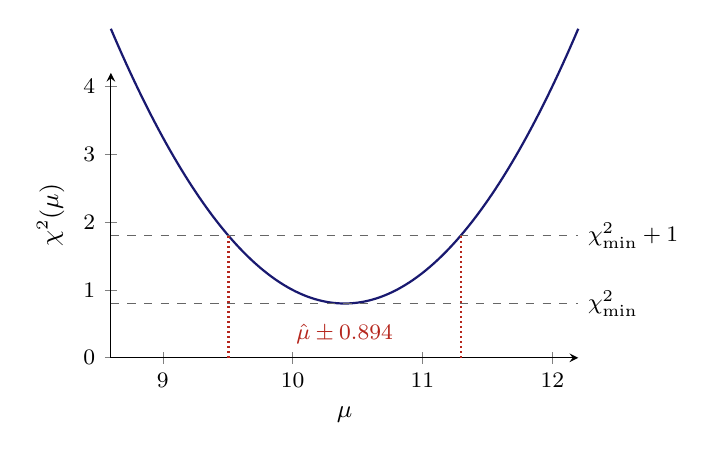
\begin{tikzpicture}
\begin{axis}[width=0.62\textwidth,height=5.2cm,xlabel={$\mu$},ylabel={$\chi^2(\mu)$},xmin=8.6,xmax=12.2,ymin=0,ymax=4.2,
  axis lines=left,tick label style={font=\footnotesize},label style={font=\small},clip=false]
\addplot[domain=8.6:12.2,samples=120,thick,MidnightBlue] {(10-x)^2+(12-x)^2/4};
\addplot[dashed,black!60] coordinates {(8.6,0.8) (12.2,0.8)};
\addplot[dashed,black!60] coordinates {(8.6,1.8) (12.2,1.8)};
\addplot[densely dotted,BrickRed,thick] coordinates {(9.5056,0) (9.5056,1.8)};
\addplot[densely dotted,BrickRed,thick] coordinates {(11.2944,0) (11.2944,1.8)};
\node[font=\footnotesize,anchor=west] at (axis cs:12.2,0.8) {$\chi^2_{\min}$};
\node[font=\footnotesize,anchor=west] at (axis cs:12.2,1.8) {$\chi^2_{\min}+1$};
\node[font=\footnotesize,BrickRed] at (axis cs:10.4,0.35) {$\hat\mu\pm0.894$};
\end{axis}
\end{tikzpicture}
\caption{Toy 1. The best value is the bottom of the parabola; the $1\sigma$ interval is where $\chi^2$ has risen by one unit.}\label{fig:pr-parabola}
\end{figure}

% ---------------------------------------------------------------------
\subsection{\texorpdfstring{What ``$\pm1\sigma$'' means}{What plus-minus one sigma means}}\label{sec:pr-sigma}
\paragraph{Coverage.} The frequentist meaning of ``$\theta=\hat\theta\pm\sigma$'' is a statement about the \emph{procedure}: if the experiment were repeated many times and each time the interval $[\hat\theta-\sigma,\hat\theta+\sigma]$ were constructed in the same way, $68.3\%$ of those intervals would contain the true value. For the straight-line toy below, a simulation with $2\times10^5$ repeated data sets gives $68.28\%$ for the slope. It does \emph{not} say that this particular interval has a $68\%$ chance of containing the truth; that is the Bayesian statement, which here happens to give the same interval.

\paragraph{One parameter versus several.} The rule ``$\Delta\chi^2=1$'' gives $68.3\%$ for \emph{one} parameter, with all others re-optimized. The region $\Delta\chi^2\le1$ in a plane of \emph{two} parameters contains the true pair only $39.3\%$ of the time (simulated: $39.5\%$); a $68.3\%$ joint region needs $\Delta\chi^2\le2.30$ (simulated: $68.6\%$). The reason: the sum of squares of two unit Gaussians is less often below one than one squared Gaussian is. The table in \S\ref{sec:cov} gives the values for up to four parameters.

\paragraph{Marginal versus conditional.} Figure~\ref{fig:pr-ellipse} shows the two ways of reading one error off a two-parameter ellipse. The \emph{marginal} error is the half-width of the shadow of the $\Delta\chi^2=1$ ellipse on the axis: the other parameter is allowed to adjust. The \emph{conditional} error is the half-width of a horizontal slice through the centre: the other parameter is frozen at its best value. Only the marginal error is an honest uncertainty; the conditional error is what you get if you vary one parameter and keep the others fixed, and it is always smaller.

% ---------------------------------------------------------------------
\subsection{Toy 2: a straight line by hand}\label{sec:pr-line}
Three points $(x,y)=(0,1),(1,2),(2,4)$, each with $\sigma=1$, and the model $\mu(x)=a+bx$.

\paragraph{Estimation.} $\chi^2(a,b)=\sum_i(y_i-a-bx_i)^2$. Setting both derivatives to zero gives the \emph{normal equations} $\sF\vth=\sJ^T\bm y$ with $\sJ=\begin{pmatrix}1&0\\1&1\\1&2\end{pmatrix}$:
\begin{gather*}
\sF=\sJ^T\sJ=\begin{pmatrix}3&3\\3&5\end{pmatrix},\qquad \sJ^T\bm y=\begin{pmatrix}7\\10\end{pmatrix},\\
\sC=\sF^{-1}=\frac16\begin{pmatrix}5&-3\\-3&3\end{pmatrix},\qquad
\begin{pmatrix}\hat a\\\hat b\end{pmatrix}=\sC\,\sJ^T\bm y=\begin{pmatrix}5/6\\3/2\end{pmatrix}.
\end{gather*}
\paragraph{Uncertainty.} $\sigma_a=\sqrt{5/6}=0.913$, $\sigma_b=\sqrt{1/2}=0.707$, $\rho_{ab}=-3/\sqrt{15}=-0.775$. Conditional errors: $1/\sqrt{\sF_{aa}}=0.577$ and $1/\sqrt{\sF_{bb}}=0.447$.
\paragraph{Testing.} Residuals $\bm y-\hat{\bm\mu}=(\frac16,-\frac13,\frac16)$, $\chi^2_{\min}=\frac16$ with $\nu=1$.

\paragraph{Why are $a$ and $b$ correlated?} The intercept $a$ is the value of the line at $x=0$, at the \emph{edge} of the data. The data pin the line down best at their centre $\bar x=1$. If the slope is increased, the line pivots about $\bar x$ and the intercept must decrease: negative correlation. Re-parametrize around the centre, $\mu=a'+b(x-1)$: then $\sF'=\diag(3,2)$, $a'=\frac73\pm0.577$, $b=\frac32\pm0.707$, and $\rho=0$. \emph{Correlations belong to the parametrization, not to the data.} In the quarkonium fits the same thing happens with $m_Q$ and the constant $c$ ($\rho=-0.987$, \S\ref{sec:worked}): both shift all masses, and the data only constrain a combination.

\paragraph{Prediction, and why correlations matter.} Predict $P=\mu(3)=a+3b=\frac{16}3=5.33$. With $\vg=(1,3)$, \eqref{eq:pr-R4} gives $\sigma_P^2=\vg^T\sC\vg=\frac16(5-18+27)=\frac73$, $\sigma_P=1.53$. Dropping the covariance would give $\sqrt{5/6+9/2}=2.31$, fifty per cent too large. In the centred parametrization, $P=a'+2b$ and $\sigma_P^2=\frac13+4\cdot\frac12=\frac73$ again, now without any correlation term: \emph{predictions do not depend on the parametrization; only the bookkeeping does.}

\begin{figure}[h]\centering
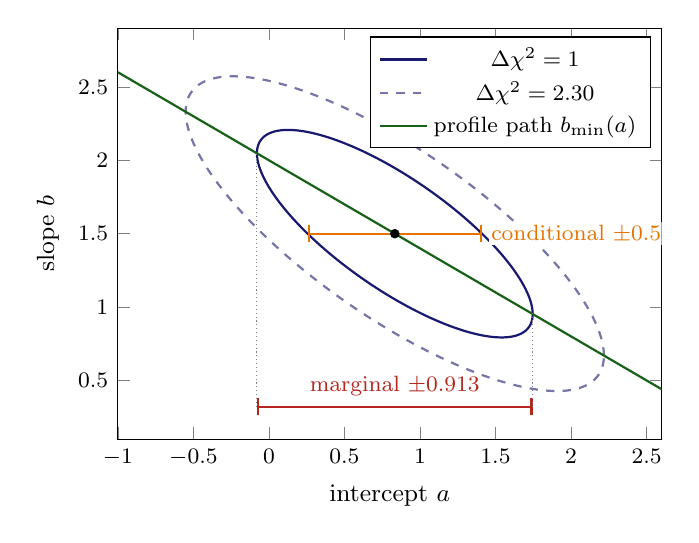
\begin{tikzpicture}
\begin{axis}[width=0.7\textwidth,height=6.8cm,xlabel={intercept $a$},ylabel={slope $b$},xmin=-1.0,xmax=2.6,ymin=0.1,ymax=2.9,
  axis lines=box,tick label style={font=\footnotesize},label style={font=\small},legend style={font=\footnotesize,at={(0.98,0.98)},anchor=north east}]
\addplot[domain=0:360,samples=200,thick,MidnightBlue,variable=\t] ({5/6+0.912871*cos(t)},{1.5-0.547723*cos(t)+0.447214*sin(t)});
\addlegendentry{$\Delta\chi^2=1$}
\addplot[domain=0:360,samples=200,thick,dashed,MidnightBlue!60,variable=\t] ({5/6+1.516575*0.912871*cos(t)},{1.5+1.516575*(-0.547723*cos(t)+0.447214*sin(t))});
\addlegendentry{$\Delta\chi^2=2.30$}
\addplot[domain=-1:2.6,samples=2,ForestGreen!70!black,thick] {(10-3*x)/5};
\addlegendentry{profile path $b_{\min}(a)$}
\addplot[only marks,mark=*,mark size=1.5pt] coordinates {(0.83333,1.5)};
\addplot[BrickRed,thick,|-|] coordinates {(-0.0795,0.32) (1.7462,0.32)};
\node[BrickRed,font=\footnotesize,anchor=south] at (axis cs:0.833,0.33) {marginal $\pm0.913$};
\addplot[densely dotted,black!50] coordinates {(-0.0795,0.32) (-0.0795,2.04)};
\addplot[densely dotted,black!50] coordinates {(1.7462,0.32) (1.7462,0.96)};
\addplot[orange!90!black,thick,|-|] coordinates {(0.2560,1.5) (1.4107,1.5)};
\node[orange!90!black,font=\footnotesize,anchor=west,fill=white,inner sep=1pt] at (axis cs:1.45,1.5) {conditional $\pm0.577$};
\end{axis}
\end{tikzpicture}
\caption{Toy 2 in the $(a,b)$ plane. The tilt of the ellipses is the correlation $\rho=-0.775$. The marginal error of $a$ is the shadow of the $\Delta\chi^2=1$ ellipse; the conditional error is the slice at fixed $b=\hat b$. The green line is the profile path: for each $a$, the $b$ that minimizes $\chi^2$; it touches the ellipse exactly at its leftmost and rightmost points, which is why the profile gives the marginal error (\S\ref{sec:cov}).}\label{fig:pr-ellipse}
\end{figure}

% ---------------------------------------------------------------------
\subsection{The geometry of least squares, and why the degrees of freedom are \texorpdfstring{$N-p$}{N-p}}\label{sec:pr-geometry}
Work with whitened data $\bm z\in\mathbb R^N$ (one axis per datum). As $\vth$ varies, the model predictions $\bm\mu(\vth)$ sweep out a $p$-dimensional surface; for a linear model it is a flat subspace, the span of the columns of $\sJ$. Minimizing $\chi^2=|\bm z-\bm\mu|^2$ means finding the point of this surface closest to the data: the \emph{orthogonal projection} (Figure~\ref{fig:pr-geom}). The residual vector is perpendicular to the surface.

Now count. The noise vector has $N$ independent unit-variance components in any orthonormal frame. Choose the frame with $p$ axes in the model surface and $N-p$ perpendicular to it. The $p$ components along the surface are absorbed by adjusting $\vth$; the $N-p$ perpendicular ones remain in the residual. Hence $\mathbb E[\chi^2_{\min}]=N-p$: each fitted parameter ``uses up'' one dimension of the noise. This is the geometric content of the hat-matrix calculation in \S\ref{sec:chi2} (the hat matrix $\sP$ is the projector onto the surface). In Toy 2, $N=3$, $p=2$: the residual lives on a line, and $\chi^2_{\min}=\frac16$ is the square of a single Gaussian-distributed number.

\begin{figure}[h]\centering
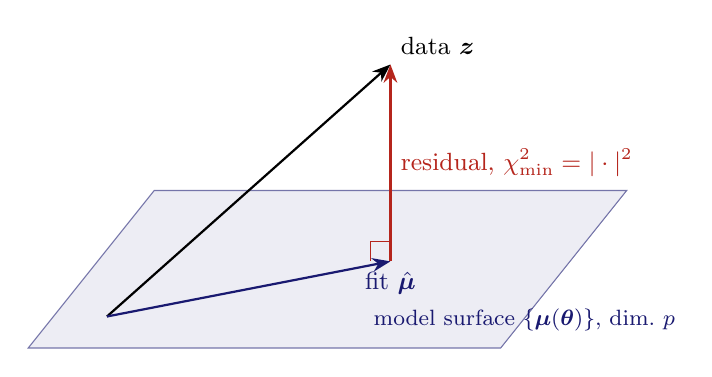
\begin{tikzpicture}[scale=1.0,>=Stealth]
\fill[MidnightBlue!8] (0,0) -- (6,0) -- (7.6,2.0) -- (1.6,2.0) -- cycle;
\draw[MidnightBlue!60] (0,0) -- (6,0) -- (7.6,2.0) -- (1.6,2.0) -- cycle;
\node[MidnightBlue,font=\footnotesize] at (6.3,0.35) {model surface $\{\bm\mu(\vth)\}$, dim.\ $p$};
\coordinate (O) at (1.0,0.4);
\coordinate (Y) at (4.6,3.6);
\coordinate (P) at (4.6,1.1);
\draw[->,thick] (O) -- (Y) node[above right,font=\small] {data $\bm z$};
\draw[->,thick,MidnightBlue] (O) -- (P) node[below,font=\small] {fit $\hat{\bm\mu}$};
\draw[->,thick,BrickRed] (P) -- (Y) node[midway,right,font=\small] {residual, $\chi^2_{\min}=|\cdot|^2$};
\draw[BrickRed] ($(P)+(0,0.25)$) -- ($(P)+(-0.25,0.25)$) -- ($(P)+(-0.25,0)$);
\end{tikzpicture}
\caption{Least squares as orthogonal projection. Of the $N$ noise directions, $p$ lie in the model surface and are absorbed by the fit; $N-p$ are perpendicular and make up $\chi^2_{\min}$.}\label{fig:pr-geom}
\end{figure}

% ---------------------------------------------------------------------
\subsection{\texorpdfstring{The $\chi^2$ distribution: which values are normal?}{The chi-squared distribution: which values are normal?}}\label{sec:pr-chi2dist}
If the model and the error model are right, $\chi^2_{\min}$ is (approximately) a sum of $\nu=N-p$ squared unit Gaussians: a $\chi^2_\nu$ variable. For one unit Gaussian $z$, $\mathbb E z^2=1$ and $\mathbb E z^4=3$, so $\operatorname{Var}z^2=2$; by (R3), $\chi^2_\nu$ has mean $\nu$ and variance $2\nu$, i.e.\ $\chi^2/\nu$ has mean $1$ and standard deviation $\sqrt{2/\nu}$.

\begin{figure}[h]\centering
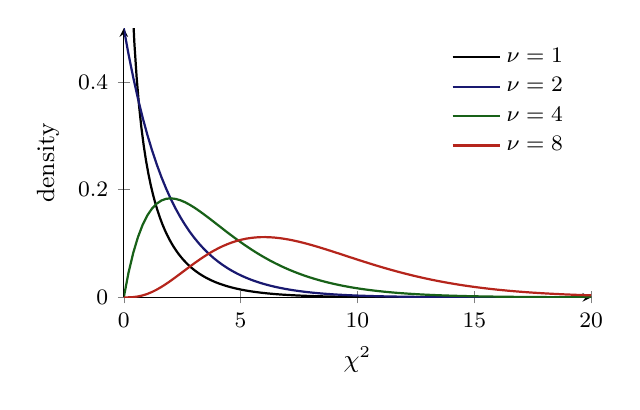
\begin{tikzpicture}
\begin{axis}[width=0.62\textwidth,height=5.0cm,xlabel={$\chi^2$},ylabel={density},xmin=0,xmax=20,ymin=0,ymax=0.5,axis lines=left,
  tick label style={font=\footnotesize},label style={font=\small},legend style={font=\footnotesize,draw=none},legend pos=north east]
\addplot[domain=0.05:20,samples=200,thick,black] {x^(-0.5)*exp(-x/2)/sqrt(2*pi)}; \addlegendentry{$\nu=1$}
\addplot[domain=0:20,samples=100,thick,MidnightBlue] {exp(-x/2)/2}; \addlegendentry{$\nu=2$}
\addplot[domain=0:20,samples=100,thick,ForestGreen!70!black] {x*exp(-x/2)/4}; \addlegendentry{$\nu=4$}
\addplot[domain=0:20,samples=100,thick,BrickRed] {x^3*exp(-x/2)/96}; \addlegendentry{$\nu=8$}
\end{axis}
\end{tikzpicture}
\caption{$\chi^2_\nu$ densities. For few degrees of freedom the distribution is broad and skewed.}\label{fig:pr-chi2}
\end{figure}

\begin{center}\small
\begin{tabular}{@{}lcccccc@{}}\toprule
$\nu$ & 1 & 2 & 4 & 8 & 20 & 100\\\midrule
central 95\% range of $\chi^2/\nu$ & 0.001--5.02 & 0.025--3.69 & 0.12--2.79 & 0.27--2.19 & 0.48--1.71 & 0.74--1.30\\\bottomrule
\end{tabular}
\end{center}
\emph{Lesson for your fits.} With eight charmonium states and four parameters ($\nu=4$), any $\chi^2/\nu$ between $0.12$ and $2.8$ is unremarkable. Do not read meaning into $\chi^2/\nu=1.6$ versus $0.9$.

\paragraph{$p$-values.} $p=P(\chi^2_\nu\ge\chi^2_{\min})$ is the probability of a misfit at least this bad \emph{if} model and errors were right. A tiny $p$ means: the model is wrong, or the errors are underestimated, or both. For quarkonium it is usually ``both'', and the theory floor is how we say so quantitatively.

\paragraph{How well is the theory floor itself known?} $\sigma_{\rm th}$ is determined from $\nu$ residuals, so it is itself uncertain. If the true floor were $\sigma$, the estimate $\sqrt{\chi^2_\nu/\nu}\,\sigma$ has, for $\nu=4$, a 16--84\% range of $0.60$--$1.28$ times $\sigma$ (simulated). Turned around: the worked example's ``$\sigma_{\rm th}=8.3\MeV$'' means ``roughly $6.5$--$14\MeV$''. Two models whose fitted floors differ by $20\%$ are not distinguishable this way.

% ---------------------------------------------------------------------
\subsection{Theory floor versus scale factor: two models of what went wrong}\label{sec:pr-floor}
Take Toy 1 with much smaller, inconsistent errors: $y_1=10.0\pm0.1$, $y_2=12.0\pm0.2$. Now $\chi^2_{\min}=80$ for $\nu=1$: the two numbers cannot both be right within their errors. The naive result $\hat\mu=10.40\pm0.09$ is absurd. There are two standard repairs, and they encode different beliefs:
\begin{itemize}[leftmargin=1.3em,itemsep=3pt]
\item \emph{Scale factor} (PDG, \S\ref{sec:chi2}): multiply all errors by $S=\sqrt{\chi^2_{\min}/\nu}=8.9$. Result $10.40\pm0.80$. The relative weights ($4:1$) are kept. Belief: ``the experimenters underestimated their errors by a common factor''.
\item \emph{Additive floor}: add $\sigma_{\rm th}$ in quadrature to both errors and choose it so that $\chi^2/\nu=1$; here $\chi^2=4/(0.05+2\sigma_{\rm th}^2)=1$ gives $\sigma_{\rm th}=1.41$. The weights become $0.504:0.496$ and $\hat\mu=10.99\pm1.00$. Belief: ``each point is off by a random amount of typical size $\sigma_{\rm th}$, \emph{independent of how precisely it was measured}''.
\end{itemize}
For a potential model the scatter comes from the model, not from the measurements: a $6\keV$ error on the $J/\psi$ mass does not make the model more accurate for the $J/\psi$. That is why \S\ref{sec:chi2} uses the additive floor. With the scale factor, the $J/\psi$ would keep $10^4$ times the weight of the $\eta_c(2S)$, and the fit would still ignore most of the spectrum.

% ---------------------------------------------------------------------
\subsection{Fitting as walking downhill}\label{sec:pr-downhill}
Think of $\chi^2(\vth)$ as a landscape over parameter space; the fit looks for its lowest point.
\begin{itemize}[leftmargin=1.3em,itemsep=3pt]
\item \emph{Gradient descent}: step in the direction of steepest descent. Safe but slow, especially in long narrow valleys, which is exactly what strongly correlated parameters produce: the gradient points across the valley, not along it, and the walker zig-zags.
\item \emph{Newton}: approximate the landscape by a paraboloid (value, gradient and curvature at the current point) and jump to the bottom of the paraboloid. Excellent near the minimum (it converges in a few steps), dangerous far from it (the paraboloid can be a poor guide and the jump can go anywhere).
\item \emph{Gauss--Newton}: Newton with the curvature estimated from first derivatives only, $\sF=\sJ^T\sW\sJ$ \eqref{eq:GN}. For least squares this is almost free and almost as good.
\item \emph{Levenberg--Marquardt} \eqref{eq:LM}: Gauss--Newton on a leash. The damping $\lambda$ is the leash: with large $\lambda$ the step is short and along the (rescaled) gradient; with small $\lambda$ it is the full Gauss--Newton jump. After a successful step the leash is loosened ($\lambda\to\lambda/10$), after a failed one it is tightened ($\lambda\to10\lambda$). The method therefore behaves like gradient descent far away and like Newton close by, without you having to decide when to switch.
\item \emph{Local versus global.} All of the above find \emph{a} minimum, the one whose basin they start in. A landscape with several valleys (GI fits with ten or more parameters) needs several starting points (\S\ref{sec:minimize}).
\end{itemize}

% ---------------------------------------------------------------------
\subsection{Beyond the parabola: profiles, bootstrap, Markov chains}\label{sec:pr-beyond}
The curvature error $\sC=\sF^{-1}$ assumes that $\chi^2$ is a paraboloid. Three tools check or replace that assumption.

\paragraph{Profile likelihood: let the others do their best.} For each fixed value of the parameter you care about, minimize $\chi^2$ over all the others, and plot the result. In Figure~\ref{fig:pr-ellipse} this is $\chi^2$ along the green line. For a linear model the profile is an exact parabola and gives the marginal error. For a non-linear model the valley is curved; the profile follows it and gives asymmetric intervals ($\Delta\chi^2=1$ crossings at different distances), which the parabola cannot.

\paragraph{Parametric bootstrap: rerun the experiment on the computer.} Take the fitted model as if it were the truth, add Gaussian noise with the data covariance, refit, and repeat a few hundred times. The spread of the refitted parameters \emph{is} the sampling distribution of $\hat\vth$, including all non-linearities, parameter boundaries and biases. It costs one fit per replica, and it answers the frequentist question directly.

\paragraph{Markov chain Monte Carlo: a walker that spends its time where the probability is.} The Metropolis rule: propose a random step; if it goes to higher posterior probability, take it; if it goes down, take it with probability $\pi_{\rm new}/\pi_{\rm old}$, otherwise stay (and count the current point again). After many steps the fraction of time spent in any region equals its posterior probability.

\begin{example}[Detailed balance with two states]
Let a ``parameter'' take two values, $A$ and $B$, with target probabilities $\pi(A)=\frac23$, $\pi(B)=\frac13$. Always propose the other state. From $A$, the move to $B$ goes downhill and is accepted with probability $\pi(B)/\pi(A)=\frac12$; from $B$ the move to $A$ goes uphill and is always accepted. In equilibrium the probability flow $A\to B$ is $\pi(A)\cdot\frac12=\frac13$ and the flow $B\to A$ is $\pi(B)\cdot1=\frac13$: they balance, so the occupation $(\frac23,\frac13)$ is stationary. Check by the transition matrix $T=\begin{pmatrix}1/2&1/2\\1&0\end{pmatrix}$: $(\frac23,\frac13)\,T=(\frac13+\frac13,\ \frac13)=(\frac23,\frac13)$. The general proof in \S\ref{sec:beyond} is this argument with integrals.
\end{example}
Practical consequences: (i) the start is arbitrary, so discard an initial \emph{burn-in}; (ii) successive samples are correlated (the walker moves a little each time), so $n$ samples are worth only $n_{\rm eff}=n/\tau_{\rm int}$ independent ones; (iii) one walker cannot tell you that it has explored everything, so run several from different starts and check that they agree ($\hat R$).

\begin{center}\small
\begin{tabular}{@{}p{3.0cm}p{5.6cm}p{6.2cm}@{}}\toprule
method & answers & use when\\\midrule
curvature $\sC=\sF^{-1}$ & local Gaussian approximation & always (cheap); sufficient if the profile is parabolic\\
profile likelihood & interval for one quantity, asymmetric if needed & key parameters; any doubt about non-linearity\\
bootstrap & frequentist sampling distribution & bias, boundaries, non-linear predictions\\
MCMC & full posterior, priors, marginals of anything & many parameters, priors/penalties, correlated predictions\\\bottomrule
\end{tabular}
\end{center}

% ---------------------------------------------------------------------
\subsection{Comparing models without fooling yourself}\label{sec:pr-compare}
More parameters always lower $\chi^2$. In Toy 2, a parabola $a+bx+cx^2$ goes exactly through all three points: $\chi^2=0$. Is it the better model?
\begin{itemize}[leftmargin=1.3em,itemsep=3pt]
\item \emph{AIC} ($\chi^2_{\min}+2p$; the expected $\chi^2$ on \emph{new} data, \S\ref{sec:modelcomp}): line $\frac16+4=4.17$, parabola $0+6=6$. The line wins.
\item \emph{BIC} ($\chi^2_{\min}+p\ln N$): line $2.36$, parabola $3.30$. The line wins.
\item \emph{Leave-one-out}: drop each point, refit the line through the other two, and predict the dropped point. By hand: without $(0,1)$ the line is $y=2x$, predicting $0$ (miss $+1$); without $(1,2)$ it is $y=1+1.5x$, predicting $2.5$ (miss $-0.5$); without $(2,4)$ it is $y=1+x$, predicting $3$ (miss $+1$). The one-fit formula \eqref{eq:loo} reproduces these exactly: the leverages are $h=(\frac56,\frac13,\frac56)$ (sum $=2=p$) and $\Delta_i/(1-h_i)=(+1,-0.5,+1)$. The parabola cannot be tested at all: with one point removed it has three parameters for two points.
\end{itemize}
The idea behind all three: a model is good if it \emph{predicts} data it has not seen, not if it \emph{reproduces} data it was tuned to. AIC estimates the prediction error from the fit itself; leave-one-out measures it; BIC asks how much of the parameter space the data actually needed (an Occam factor). The leverage $h_i$ tells you how much datum $i$ pulled the fit towards itself: the two end points of the line ($h=\frac56$) control the slope, the middle point ($h=\frac13$) hardly matters.

% ---------------------------------------------------------------------
\subsection{The error budget as a story}\label{sec:pr-budget}
A number without its error budget cannot be used by anybody else. Tell the story of every error source separately (\S\ref{sec:errors}):
\begin{itemize}[leftmargin=1.3em,itemsep=3pt]
\item \emph{Parametric (statistical)}: ``given this model and this error model, the data allow the parameters to move this much''. It shrinks with better data.
\item \emph{Numerical}: ``our own approximations (basis size, quadrature) move the result this much''. You control it; make it negligible ($\le1\%$ of the smallest experimental error) and say so.
\item \emph{Theory floor}: ``this model misses masses by about this much''. It does not shrink with better data.
\item \emph{Ambiguities}: ``choices the model does not fix (which $M$ in a width formula, the scale of $\as$) move the result this much''.
\item \emph{Model spread}: ``other reasonable Hamiltonians give this range''.
\end{itemize}
Add in quadrature only errors that are independent and roughly Gaussian (parametric and numerical, say). Keep the others separate so that a reader sees which one dominates. Example from the worked fit: for $\Gamma_{ee}(J/\psi)$ the parametric error is $\pm1.1\keV$, the choice of $M$ moves it by $1.3\keV$, and the QCD factor $(1-\frac{16\as}{3\pi})$ ranges from $0.09$ to about $0.4$ depending on which $\as$ is used: the last item dominates everything, and only a separate budget shows it.

% ---------------------------------------------------------------------
\subsection{Ten common mistakes}\label{sec:pr-mistakes}
\begin{enumerate}[leftmargin=1.8em,itemsep=2pt]
\item Fitting with experimental errors only, when the model cannot reach that precision (\S\ref{sec:pr-floor}).
\item Quoting conditional errors (others fixed) instead of marginal ones (Figure~\ref{fig:pr-ellipse}).
\item Combining errors of two predictions without their covariance, e.g.\ for a splitting (\S\ref{sec:pr-line}).
\item Over-interpreting $\chi^2/\nu$ with few degrees of freedom (\S\ref{sec:pr-chi2dist}).
\item Reading a two-parameter $\Delta\chi^2=1$ contour as a 68\% region (\S\ref{sec:pr-sigma}).
\item Re-optimizing the basis during the fit, which makes $\chi^2(\vth)$ noisy (\S\ref{sec:hyper}).
\item Fitting states above the open-flavour threshold with the same floor as those below (\S\ref{sec:fitsetup}).
\item Not knowing what your tool does by default: Mathematica's \texttt{NonlinearModelFit} rescales the parameter errors by $\sqrt{\chi^2/\nu}$ unless told not to (\S\ref{sec:mma-stats}); Ceres reports $\frac12\chi^2$ as its cost.
\item Running a Markov chain without convergence diagnostics, or reporting $n$ instead of $n_{\rm eff}$.
\item Adding the model spread in quadrature to the statistical error.
\end{enumerate}
\section{Fitting, statistics and error analysis}\label{sec:stats}

If the statistical way of thinking is not yet second nature, read the primer (\S\ref{sec:primer}) first: it explains every idea of this section on two toy problems you can do by hand. Each subsection below has an ``In plain words'' box that points back to it.

Up to now the parameters of each Hamiltonian were given. In the project you will \emph{determine} them from data, together with their uncertainties, and then propagate those uncertainties to predictions. This section derives every statistical tool you need, in the order you will use them. A complete worked example (Model A fitted to the charmonium states below open-charm threshold) is in \S\ref{sec:worked}; every method below is illustrated there with numbers you can reproduce.

\paragraph{Notation (sans-serif = statistics matrices).} Data $y_i$, $i=1,\dots,N$; model predictions $\mu_i(\vth)$ (eigenvalues, or observables computed from eigenvectors); parameters $\vth=(\theta_1,\dots,\theta_p)$; residuals $\Delta_i(\vth)=y_i-\mu_i(\vth)$; data covariance $\sV$ and weight matrix $\sW=\sV^{-1}$; Jacobian $\sJ_{ia}=\partial\mu_i/\partial\theta_a$; Fisher matrix $\sF=\sJ^T\sW\sJ$; parameter covariance $\sC$. Bold upright $\mH,\mS$ remain the GEM matrices.

% ---------------------------------------------------------------------
\subsection{What is fitted, and to what}\label{sec:fitsetup}
\paragraph{Two kinds of parameters.} They are listed in Table~\ref{tab:twokinds}.
\begin{table}[ht]\centering\small
\begin{tabular}{@{}p{2.6cm}p{6.5cm}p{5.6cm}@{}}\toprule
 & physics parameters $\vth$ & basis hyperparameters $\bm\xi$\\\midrule
Model A & $m_Q$, $\as$ (or $\kappa$), $b$, $c$, $\sigma$ (smearing of the contact term) & per channel: $n_{\max},r_1,r_{\max}$; complex-range set $(\rho_1,\rho_{\max},\omega)$; threshold $\eta$\\
Model B & A $+\ \mus$ & same\\
Model C & $m_q$, $b$, $c$, $\sigma_0$, $s$, $\epsilon_{c},\epsilon_{sov},\epsilon_t,\epsilon_{sos}$; optionally $\{\alpha_k,\gamma_k\}$ (\S\ref{sec:alphafit}) & same $+$ quadrature settings for the $p$ integrals\\
Model D & C $+\ \mus$ & same\\\bottomrule
\end{tabular}
\caption{Physics parameters and basis hyperparameters of the four models.}\label{tab:twokinds}
\end{table}
They are treated completely differently. $\vth$ is \emph{inferred from data} and carries statistical uncertainty. $\bm\xi$ is \emph{not physics}: it is chosen by the variational principle (\S\ref{sec:hyper}), it is never fitted to data, and its only footprint on the result is a numerical error $\sigma_{\rm num}$ (\S\ref{sec:errors}).

\paragraph{Which data.} A potential model with a $Q\bar Q$ Fock space only knows about states that cannot decay into open flavour. Above the threshold ($D\bar D$ at $\approx3.73\GeV$, $B\bar B$ at $\approx10.56\GeV$) the coupling to meson--meson channels shifts masses by tens of MeV, which the model does not contain. Standard practice:
\begin{itemize}[leftmargin=1.3em,itemsep=2pt]
\item fit to the well-established states \emph{below} threshold;
\item use states above threshold only as \emph{predictions} (and expect deviations of the size of coupled-channel shifts);
\item if you fit them anyway, give them a larger theory floor (below).
\end{itemize}
For charmonium this leaves the eight states of Table~\ref{tab:ccdata}.

\begin{table}[h]\centering\small
\begin{tabular}{@{}llllc@{}}\toprule
state & $n^{2S+1}L_J$ & $(L,S,J)$, radial index & mass (MeV) & used in fit\\\midrule
$\eta_c(1S)$ & $1^1S_0$ & $(0,0,0)$, 1st & $2984.09\pm0.30$ & yes\\
$J/\psi$ & $1^3S_1$ & $(0,1,1)$, 1st & $3096.900\pm0.006$ & yes\\
$\chi_{c0}(1P)$ & $1^3P_0$ & $(1,1,0)$, 1st & $3415.50\pm0.19$ & yes\\
$\chi_{c1}(1P)$ & $1^3P_1$ & $(1,1,1)$, 1st & $3510.67\pm0.05$ & yes\\
$h_c(1P)$ & $1^1P_1$ & $(1,0,1)$, 1st & $3525.37\pm0.14$ & yes\\
$\chi_{c2}(1P)$ & $1^3P_2$ & $(1,1,2)$, 1st & $3556.17\pm0.07$ & yes\\
$\eta_c(2S)$ & $2^1S_0$ & $(0,0,0)$, 2nd & $3637.8\pm0.6$ & yes\\
$\psi(2S)$ & $2^3S_1$ & $(0,1,1)$, 2nd & $3686.097\pm0.010$ & yes\\\bottomrule
\end{tabular}
\caption{Charmonium states below the $D\bar D$ threshold; PDG averages as listed in pdgLive (accessed October 2026). Check the current values before your final fits.}\label{tab:ccdata}
\end{table}

\paragraph{Level identification.} Each datum must be attached to a definite eigenvalue: channel $(L,S,J)$ and radial index $n$. In a coupled channel ($L=J\mp1$) the eigenvector has both components; label each eigenvalue by its dominant component, $P_D=\vc_D^T\mS^D\vc_D$ (\S\ref{sec:observables}). During a fit the ordering can change (an $S$-dominated and a $D$-dominated level can cross as parameters move). Track levels by \emph{maximum overlap}: at the new parameter point choose the eigenvector $\vc'_b$ maximizing $|\vc'^T_b\mS\vc_a|$ with the old one. With a fixed basis, $\mS$ is the same at both points, so this is one matrix--vector product.

% ---------------------------------------------------------------------
\subsection{\texorpdfstring{From the likelihood to $\chi^2$}{From the likelihood to chi-squared}}\label{sec:chi2}
\subsubsection{Independent Gaussian errors}
\textbf{Step 1 (model for the data).} Write each measurement as truth plus noise, and the truth as model plus model error:
\begin{equation}
y_i=\mu_i(\vth)+\varepsilon_i^{\rm exp}+\varepsilon_i^{\rm th},\qquad \varepsilon_i^{\rm exp}\sim\mathcal N(0,\sigma_{{\rm exp},i}^2),\quad \varepsilon_i^{\rm th}\sim\mathcal N(0,\sigma_{{\rm th},i}^2).
\end{equation}
The sum of two independent Gaussians is Gaussian with the variances added: $y_i-\mu_i\sim\mathcal N(0,s_i^2)$, $s_i^2=\sigma_{{\rm exp},i}^2+\sigma_{{\rm th},i}^2$.

\textbf{Step 2 (likelihood).} The probability density of the observed data as a function of $\vth$:
\begin{equation}
L(\vth)=\prod_{i=1}^N\frac{1}{\sqrt{2\pi s_i^2}}\exp\Big[-\frac{(y_i-\mu_i(\vth))^2}{2s_i^2}\Big].
\end{equation}
\textbf{Step 3 (log).} Products become sums:
\begin{equation}
-2\ln L(\vth)=\underbrace{\sum_{i=1}^N\frac{(y_i-\mu_i(\vth))^2}{s_i^2}}_{\chi^2(\vth)}+\sum_{i=1}^N\ln(2\pi s_i^2).
\label{eq:m2lnL}
\end{equation}
\textbf{Step 4.} If the $s_i$ do not depend on $\vth$, the second sum is a constant: \emph{maximizing the likelihood is minimizing $\chi^2$}. The maximum-likelihood estimate is $\hat\vth=\arg\min\chi^2$.
\begin{plainwords}[In plain words]
$\chi^2$ measures, for each datum, by how many standard deviations the prediction misses it, squares, and adds. Minimizing it means choosing the parameters under which the observed data would have been most probable. Toy~1 (Example~\ref{ex:wmean}) does this by hand for a weighted mean.
\end{plainwords}

\subsubsection{Correlated errors}
If the noise vector has covariance $\sV$ (symmetric, positive definite), the multivariate Gaussian density is $(2\pi)^{-N/2}(\det\sV)^{-1/2}\exp[-\frac12\vD^T\sV^{-1}\vD]$, so
\begin{equation}
\chi^2(\vth)=\vD^T\sW\vD,\qquad \sW=\sV^{-1},\qquad \vD=\bm y-\bm\mu(\vth).
\label{eq:chi2corr}
\end{equation}
For diagonal $\sV=\diag(s_i^2)$ this is the previous formula.

\begin{example}[Fitting splittings instead of masses]
Suppose you fit differences $d_i=y_i-y_0$ to a reference state (to remove the constant $c$, or because the splittings are what you trust). If the $y$'s are independent with variances $s_i^2$, then
\[
\operatorname{Cov}(d_i,d_j)=\operatorname{Cov}(y_i-y_0,\,y_j-y_0)=\delta_{ij}s_i^2+s_0^2 ,
\]
because the common $y_0$ appears in both. So the splittings are correlated and you must use \eqref{eq:chi2corr} with $\sV_{ij}=\delta_{ij}s_i^2+s_0^2$; ignoring the off-diagonal $s_0^2$ double-counts the reference state.
\end{example}

\subsubsection{Why a theory floor is unavoidable}
Experimental mass errors range from $6\keV$ ($J/\psi$) to $0.6\MeV$ ($\eta_c(2S)$); no potential model is accurate to $6\keV$. With $s_i=\sigma_{{\rm exp},i}$ alone the weights $1/s_i^2$ differ by $10^4$, and the fit simply reproduces the two most precise states and ignores the others. In the worked example, the fit with experimental errors only has $\chi^2=10\,011$ for $\nu=4$ and residuals of $0.004$ and $0.009\MeV$ for $J/\psi$ and $\psi(2S)$ but $-17\MeV$ for $\chi_{c0}$. The theory floor $\sigma_{\rm th}$ states how well the model \emph{can} work and restores sensible weights.

\paragraph{Three ways to set $\sigma_{\rm th}$.}
\begin{enumerate}[leftmargin=1.5em,itemsep=2pt]
\item \emph{A priori}: from the size of what the model neglects (e.g.\ the next order in $v^2$; \S\ref{sec:errors}). Usually conservative.
\item \emph{A posteriori}: choose $\sigma_{\rm th}$ (common to all states) such that $\chi^2_{\min}/\nu=1$, $\nu=N-p$.
\item \emph{As a fitted nuisance parameter}: maximize the full likelihood \eqref{eq:m2lnL}, including the $\ln s_i^2$ term (which now depends on $\sigma_{\rm th}$).
\end{enumerate}
Options 2 and 3 are closely related, as the next derivation shows.

\begin{result}[Maximum-likelihood theory floor]
Take $s_i^2=\sigma_{{\rm exp},i}^2+\sigma_{\rm th}^2$ and differentiate \eqref{eq:m2lnL} with respect to $\sigma_{\rm th}^2$ at fixed $\vth$:
\[
\frac{\partial(-2\ln L)}{\partial\sigma_{\rm th}^2}=\sum_i\Big[-\frac{\Delta_i^2}{s_i^4}+\frac1{s_i^2}\Big]=0
\quad\Longrightarrow\quad
\sum_i\frac{\Delta_i^2-s_i^2}{s_i^4}=0 .
\]
When $\sigma_{\rm th}\gg\sigma_{\rm exp}$ all $s_i$ are equal and this gives $\sigma_{\rm th}^2=\frac1N\sum_i\Delta_i^2$.
\end{result}
\paragraph{Bias of the ML estimate, and the $N-p$.} For a model linear in $\vth$ (or linearized at $\hat\vth$) with equal errors $\sigma$, the fitted residuals are $\hat\vD=(\sI-\sP)\bm\varepsilon$, where $\sP=\sJ(\sJ^T\sJ)^{-1}\sJ^T$ is the projector onto the columns of $\sJ$ (the ``hat matrix'': $\hat{\bm\mu}=\sP\bm y$). Then
\[
\mathbb E\big[\hat\vD^T\hat\vD\big]=\mathbb E\big[\bm\varepsilon^T(\sI-\sP)\bm\varepsilon\big]=\sigma^2\operatorname{tr}(\sI-\sP)=\sigma^2(N-p),
\]
using $(\sI-\sP)^T(\sI-\sP)=\sI-\sP$ (projector), $\mathbb E[\varepsilon_i\varepsilon_j]=\sigma^2\delta_{ij}$, and $\operatorname{tr}\sP=\operatorname{tr}[(\sJ^T\sJ)^{-1}\sJ^T\sJ]=\operatorname{tr}\sI_p=p$. So $\frac1N\sum\Delta_i^2$ underestimates $\sigma^2$ and the unbiased estimate is $\sigma_{\rm th}^2=\frac{1}{N-p}\sum_i\hat\Delta_i^2$, which is \emph{exactly} the condition $\chi^2_{\min}/\nu=1$ of option 2. Fitting the parameters ``uses up'' $p$ degrees of freedom of the residuals.

\paragraph{Consequences.}
\begin{itemize}[leftmargin=1.3em,itemsep=2pt]
\item Once $\sigma_{\rm th}$ is tuned to give $\chi^2/\nu=1$, the $\chi^2$ value carries \emph{no} goodness-of-fit information; the information is in $\sigma_{\rm th}$ itself (``this model describes the spectrum to $\pm\sigma_{\rm th}$''). Compare models by their $\sigma_{\rm th}$ (or with a common fixed $\sigma_{\rm th}$, \S\ref{sec:modelcomp}).
\item Determine $\sigma_{\rm th}$ iteratively: fit at a trial value, solve $\sum_i\Delta_i^2/(\sigma_{{\rm exp},i}^2+\sigma_{\rm th}^2)=\nu$ for $\sigma_{\rm th}$ with the residuals fixed (one-dimensional root), refit; it converges in a few iterations.
\item State-dependent floors are reasonable (e.g.\ larger for $2S$ than $1S$, or $\sigma_{{\rm th},i}\propto\langle v^2\rangle_i$); but every extra choice is a modelling decision you must report.
\end{itemize}
\begin{plainwords}[In plain words]
$\sigma_{\rm th}$ answers ``how far off is this model, typically?''. It is the rms residual, with $N-p$ instead of $N$ because the fit has already bent towards the data (\S\ref{sec:pr-geometry}). It is added in quadrature, not multiplied, because the misfit comes from the model and does not care how precisely a state was measured (\S\ref{sec:pr-floor}). And it is itself uncertain: with $\nu=4$, by roughly $\pm35\%$ (\S\ref{sec:pr-chi2dist}).
\end{plainwords}

\paragraph{The PDG scale factor (Birge ratio).} When a fit with \emph{fixed} errors gives $\chi^2/\nu>1$, a common practice is to multiply all parameter errors by $S=\sqrt{\chi^2_{\min}/\nu}$. This is equivalent to scaling all $s_i$ by $S$, which leaves $\hat\vth$ unchanged and restores $\chi^2/\nu=1$. It is the same idea as option 2 applied multiplicatively instead of in quadrature.

% ---------------------------------------------------------------------
\subsection{Finding the minimum}\label{sec:minimize}
\subsubsection{Gradient and Hessian of \texorpdfstring{$\chi^2$}{chi-squared}}
Differentiate $\chi^2=\vD^T\sW\vD$ with $\partial\vD/\partial\theta_a=-\sJ_{\cdot a}$:
\begin{align}
\frac{\partial\chi^2}{\partial\theta_a}&=-2\,(\sJ^T\sW\vD)_a,\label{eq:gradchi}\\
\frac{\partial^2\chi^2}{\partial\theta_a\partial\theta_b}&=2\,(\sJ^T\sW\sJ)_{ab}-2\sum_{ij}\Delta_i\sW_{ij}\frac{\partial^2\mu_j}{\partial\theta_a\partial\theta_b}.\label{eq:hesschi}
\end{align}
The second term is a sum of residuals times curvatures. Near a good minimum the residuals are small and of random sign, so it is small compared with the first; dropping it gives the \emph{Gauss--Newton Hessian} $2\sF$, $\sF=\sJ^T\sW\sJ$, which is positive semi-definite by construction and needs only first derivatives.

\subsubsection{Gauss--Newton step}
Linearize the model around the current point, $\bm\mu(\vth+\bm\delta)\simeq\bm\mu(\vth)+\sJ\bm\delta$; then
$\chi^2(\vth+\bm\delta)\simeq(\vD-\sJ\bm\delta)^T\sW(\vD-\sJ\bm\delta)$, a quadratic in $\bm\delta$. Setting its gradient to zero:
\begin{equation}
-2\sJ^T\sW(\vD-\sJ\bm\delta)=0\quad\Longrightarrow\quad \sF\,\bm\delta=\sJ^T\sW\vD .
\label{eq:GN}
\end{equation}
Iterate $\vth\to\vth+\bm\delta$. Gauss--Newton converges quadratically near the minimum but can overshoot far from it.

\subsubsection{Levenberg--Marquardt}
Add a damping term:
\begin{equation}
\big(\sF+\lambda\,\sD\big)\bm\delta=\sJ^T\sW\vD,\qquad \sD=\diag(\sF).
\label{eq:LM}
\end{equation}
For $\lambda\to0$ this is Gauss--Newton; for $\lambda\to\infty$, $\bm\delta\to\frac1\lambda\sD^{-1}\sJ^T\sW\vD=-\frac1{2\lambda}\sD^{-1}\nabla\chi^2$, a short steepest-descent step (scaled per parameter by $\sD$, which makes it invariant under rescaling of individual parameters). Equation~\eqref{eq:LM} is the exact minimizer of the linearized $\chi^2$ under a constraint on the step length $\|\sD^{1/2}\bm\delta\|$ (Lagrange multiplier $\lambda$), so it is a trust-region method. Algorithm: accept the step and set $\lambda\to\lambda/10$ if $\chi^2$ decreased; otherwise reject and set $\lambda\to10\lambda$. Stop when the relative change of $\chi^2$ is below $10^{-10}$ or so.
\begin{plainwords}[In plain words]
Gauss--Newton jumps to the bottom of the local paraboloid; Levenberg--Marquardt is Gauss--Newton on a leash $\lambda$ that is loosened after every success and tightened after every failure (\S\ref{sec:pr-downhill}). The $\sD$ scaling makes the leash the same length for $m_Q\sim1.5$ and $\epsilon\sim0.02$. Algorithm~\ref{alg:lm} in \S\ref{sec:blueprint} is the version to implement.
\end{plainwords}

\subsubsection{The Jacobian from Feynman--Hellmann}
For a mass, $\mu_i=\mathcal E_{k(i)}$ (plus $m_1+m_2$ in Models A/B), and \eqref{eq:FH} with a fixed basis ($\mS'=0$) gives
\begin{equation}
\sJ_{ia}=\vc_{k(i)}^T\,\frac{\partial\mH}{\partial\theta_a}\,\vc_{k(i)}\qquad(+\,\partial(m_1+m_2)/\partial\theta_a).
\end{equation}
One diagonalization per channel gives the full Jacobian (one matrix $\partial\mH/\partial\theta_a$ per parameter, listed in \S\ref{sec:derivs}), against $2p$ extra diagonalizations for central finite differences. For observables built from eigenvectors use \eqref{eq:dvec}. For perturbative shifts $\vc^T\mH_1\vc$ (as for the spin--orbit and tensor terms in Model A) the derivative is $\vc^T\mH_1'\vc+2\vc^T\mH_1\vc'$ with $\vc'$ from \eqref{eq:dvec}. Always check the analytic Jacobian against finite differences once (worked example: $\partial M_{J/\psi}/\partial b=\langle r\rangle=1.88670872$ by both).

\subsubsection{Practicalities}
\begin{itemize}[leftmargin=1.3em,itemsep=2pt]
\item \emph{Fixed basis during the fit} (Property 5 of \S\ref{sec:hyper}): otherwise $\chi^2(\vth)$ is not smooth.
\item \emph{Scaling and positivity.} Parameters have very different sizes ($m_Q\sim1.5$, $b\sim0.15$, $\epsilon_x\sim0.02$). Fit in $\ln m_Q,\ln b,\ln\sigma,\ln\mus$ (positive by construction), or in units of a typical scale. Errors transform with the Jacobian of the reparametrization: if $\bm\phi=\bm\phi(\vth)$ then $\sC_\phi=\sK\sC_\theta\sK^T$, $\sK_{ab}=\partial\phi_a/\partial\theta_b$ (derived in \S\ref{sec:propagate}).
\item \emph{Global search.} For Models C/D (10+ parameters) $\chi^2$ is multimodal. Use a global stage (multistart from a Latin hypercube, differential evolution, or CMA-ES) to find the basin, then polish with Levenberg--Marquardt. Report whether different starts converge to the same $\hat\vth$.
\item \emph{Sanity bounds.} Reject parameter points where the Hamiltonian becomes unbounded or unphysical (e.g.\ $\mus<0$, negative smearing widths); return $\chi^2=+\infty$ there.
\end{itemize}

% ---------------------------------------------------------------------
\subsection{Parameter uncertainties from the curvature}\label{sec:cov}
\subsubsection{Derivation 1: Gaussian approximation to the likelihood}
Expand $\chi^2$ around its minimum, where the gradient vanishes, and use the Gauss--Newton Hessian:
\begin{equation}
\chi^2(\vth)\simeq\chi^2_{\min}+(\vth-\hat\vth)^T\sF(\vth-\hat\vth).
\end{equation}
Then $L\propto\ee^{-\chi^2/2}\propto\exp\big[-\frac12(\vth-\hat\vth)^T\sF(\vth-\hat\vth)\big]$, a Gaussian in $\vth$ whose covariance is the inverse of the matrix in the exponent:
\begin{equation}
\boxed{\ \sC=\sF^{-1}=(\sJ^T\sW\sJ)^{-1}=\Big(\tfrac12\nabla\nabla\chi^2\Big)^{-1}\ }
\label{eq:cov}
\end{equation}
(note the factor $\frac12$ if you use the numerical Hessian of $\chi^2$).
\begin{plainwords}[In plain words]
A sharply curved minimum means well-determined parameters. In Toy~1 the curvature $\sum1/\sigma_i^2=1.25$ gives $\sigma=1/\sqrt{1.25}=0.894$; in Toy~2 the inverse of $\sF$ gives the whole error ellipse (\S\ref{sec:pr-line}). The two derivations below say the same thing in the two languages of \S\ref{sec:pr-mindset}: width of the likelihood, and spread of $\hat\vth$ over repeated experiments.
\end{plainwords}

\subsubsection{Derivation 2: propagation of the data noise}
Linearize the Gauss--Newton solution around the truth $\vth_0$: $\hat\vth-\vth_0=\sA(\bm y-\bm\mu(\vth_0))$, $\sA=\sF^{-1}\sJ^T\sW$, which is linear in the noise $\bm\varepsilon=\bm y-\bm\mu(\vth_0)$ with $\operatorname{Cov}(\bm\varepsilon)=\sV=\sW^{-1}$. For any linear map, $\operatorname{Cov}(\sA\bm\varepsilon)=\sA\sV\sA^T$:
\[
\operatorname{Cov}(\hat\vth)=\sF^{-1}\sJ^T\sW\,\sW^{-1}\,\sW\sJ\sF^{-1}=\sF^{-1}(\sJ^T\sW\sJ)\sF^{-1}=\sF^{-1}.
\]
Both derivations give the same $\sC$: it is the frequentist spread of $\hat\vth$ over repeated experiments \emph{and} the width of the likelihood.

\subsubsection{\texorpdfstring{Why $\Delta\chi^2=1$: the profile of one parameter}{Why Delta chi-squared = 1: the profile of one parameter}}
Split $\bm\delta=\vth-\hat\vth=(\delta_1,\bm\delta_2)$, with $\delta_1$ the parameter of interest and $\bm\delta_2$ the rest, and $\sF$ correspondingly into blocks. Minimize the quadratic $\chi^2$ over $\bm\delta_2$ at fixed $\delta_1$:
\[
\frac{\partial}{\partial\bm\delta_2}\big[\sF_{11}\delta_1^2+2\delta_1\sF_{12}\bm\delta_2+\bm\delta_2^T\sF_{22}\bm\delta_2\big]=2\sF_{21}\delta_1+2\sF_{22}\bm\delta_2=0
\quad\Rightarrow\quad \bm\delta_2=-\sF_{22}^{-1}\sF_{21}\delta_1 .
\]
Substituting back,
\begin{equation}
\chi^2_{\rm prof}(\theta_1)=\chi^2_{\min}+\delta_1^2\big(\sF_{11}-\sF_{12}\sF_{22}^{-1}\sF_{21}\big)
=\chi^2_{\min}+\frac{\delta_1^2}{\sC_{11}},
\end{equation}
where the last step is the block-inversion (Schur complement) formula
\[
(\sF^{-1})_{11}=\big(\sF_{11}-\sF_{12}\sF_{22}^{-1}\sF_{21}\big)^{-1}.
\]
Hence the profile rises by one unit exactly at $\delta_1=\pm\sqrt{\sC_{11}}$: \emph{the $68.3\%$ interval for one parameter, with all others re-optimized, is $\Delta\chi^2=1$}.

\paragraph{Marginal versus conditional errors.} If instead you vary $\theta_1$ with the others \emph{fixed} at $\hat\vth$, $\chi^2$ rises as $\sF_{11}\delta_1^2$, giving the conditional error $1/\sqrt{\sF_{11}}\le\sqrt{\sC_{11}}$. The two coincide only without correlations. In the worked example the conditional error on $m_c$ is $1.7\MeV$, the marginal one $21\MeV$: quoting the conditional error would be a factor twelve too optimistic.
Figure~\ref{fig:pr-ellipse} shows the two readings on Toy~2: the marginal error is the shadow of the ellipse, the conditional error the slice through its centre.

\paragraph{Joint regions.} For $k$ parameters jointly, $\Delta\chi^2$ follows a $\chi^2_k$ distribution; the contour $\chi^2=\chi^2_{\min}+\Delta$ contains the true values with probability:
\begin{center}\small
\begin{tabular}{@{}lcccc@{}}\toprule
$k$ & 1 & 2 & 3 & 4\\\midrule
$68.27\%$ & 1.00 & 2.30 & 3.53 & 4.72\\
$95.45\%$ & 4.00 & 6.18 & 8.02 & 9.72\\\bottomrule
\end{tabular}
\end{center}

\subsubsection{Correlations and degeneracies}
The correlation matrix $\rho_{ab}=\sC_{ab}/\sqrt{\sC_{aa}\sC_{bb}}$ is the first thing to look at after a fit. $|\rho|\gtrsim0.95$ signals a near-degeneracy. A cleaner diagnosis uses the eigen-decomposition of the (dimensionless) Fisher matrix,
\begin{equation}
\tilde\sF=\sD_\theta\sF\sD_\theta=\sum_k\lambda_k\,\bm u_k\bm u_k^T,\qquad \sD_\theta=\diag(\hat\theta_a),
\end{equation}
in relative variables $\delta\theta_a/\hat\theta_a$. The combination $\bm u_k^T(\delta\theta/\hat\theta)$ is determined to $\pm1/\sqrt{\lambda_k}$. Small $\lambda_k$ = a direction the data barely constrain; the components of $\bm u_k$ tell you which parameters move together. Typical degeneracies in quarkonium fits:
\begin{itemize}[leftmargin=1.3em,itemsep=2pt]
\item $m_Q$ and $c$ in Models A/B: $M=2m_Q+c+\mathcal E(m_Q)$, and $\partial\mathcal E/\partial m_Q=-\langle T\rangle/m_Q$ (Feynman--Hellmann on $p^2/2\mr$) varies only mildly between states, so a change of $m_Q$ is almost compensated by $c$. Worked example: $\rho(m_c,c)=-0.987$.
\item $\as$ and $b$: both shape the potential at $r\sim0.3$--$0.6\fm$, where the low states live.
\item In GI: $\gamma_k$ and $\sigma_{12}$ enter the Coulomb-generated terms only through $\tau_k$ (\S\ref{sec:alphafit}); the $\epsilon_x$ with the smearing parameters.
\end{itemize}
Remedies: fix one parameter of the degenerate pair (and say so), add data that break the degeneracy (decay widths are sensitive to $|R(0)|^2$, i.e.\ to the short-distance potential), or add a prior (\S\ref{sec:beyond}).

% ---------------------------------------------------------------------
\subsection{Propagating to predictions}\label{sec:propagate}
\begin{result}[Linear error propagation]
Let $P(\vth)$ be a prediction (a mass of a state not in the fit, a splitting, a width) and $\vg=\nabla_\theta P(\hat\vth)$. To first order $P(\vth)-P(\hat\vth)=\vg^T(\vth-\hat\vth)$, so
\begin{equation}
\sigma^2(P)=\mathbb E\big[\vg^T\bm\delta\bm\delta^T\vg\big]=\vg^T\sC\vg,\qquad
\operatorname{Cov}(P,Q)=\vg_P^T\sC\vg_Q .
\label{eq:prop}
\end{equation}
\end{result}
\begin{itemize}[leftmargin=1.3em,itemsep=2pt]
\item The gradients come from \eqref{eq:FH} (masses) or \eqref{eq:dvec} (wave-function observables), or from central differences.
\item Correlations matter for differences: $\sigma^2(P-Q)=\sigma^2(P)+\sigma^2(Q)-2\operatorname{Cov}(P,Q)$. Always propagate the splitting as one quantity rather than combining the two individual errors.
\item For a \emph{predicted mass} to be compared with experiment, the total error is $\sqrt{\vg^T\sC\vg+\sigma_{\rm th}^2}$: the theory floor applies to new states as well.
\item The same formula transforms covariances under reparametrization: with $\bm\phi(\vth)$ and $\sK=\partial\bm\phi/\partial\vth$, $\sC_\phi=\sK\sC\sK^T$.
\item If $P$ is strongly non-linear over the $1\sigma$ region (check: compare $P(\hat\vth\pm\sqrt{\sC_{aa}}\hat{\bm e}_a)$ with the linear prediction), use the profile likelihood or sampling methods below.
\end{itemize}
\begin{plainwords}[In plain words]
Linearize the prediction and apply rule (R4) of \S\ref{sec:pr-rules}. The covariance terms are not optional: in Toy~2 the prediction at $x=3$ has error $1.53$ with them and $2.31$ without (\S\ref{sec:pr-line}).
\end{plainwords}

% ---------------------------------------------------------------------
\subsection{Beyond the quadratic approximation}\label{sec:beyond}
\subsubsection{Profile likelihood for a derived quantity}
Define
\begin{equation}
\chi^2_{\rm prof}(\psi)=\min_{\vth:\ P(\vth)=\psi}\chi^2(\vth),\qquad \text{68\% interval: }\{\psi:\ \chi^2_{\rm prof}(\psi)\le\chi^2_{\min}+1\}.
\end{equation}
\emph{Check against \eqref{eq:prop}.} In the quadratic/linear approximation minimize $\bm\delta^T\sF\bm\delta$ subject to $\vg^T\bm\delta=\Delta\psi$ with a Lagrange multiplier: $\sF\bm\delta=\lambda\vg\Rightarrow\bm\delta=\lambda\sC\vg$; the constraint gives $\lambda=\Delta\psi/\vg^T\sC\vg$; then $\Delta\chi^2=\bm\delta^T\sF\bm\delta=\lambda^2\vg^T\sC\vg=\Delta\psi^2/\vg^T\sC\vg$. So $\Delta\chi^2=1$ at $\Delta\psi=\pm\sqrt{\vg^T\sC\vg}$, as it should be. Beyond that approximation the profile gives asymmetric intervals and is reparametrization invariant.
\emph{Implementation:} for a parameter, fix it on a grid and refit the others; for a derived quantity, minimize $\chi^2+(P(\vth)-\psi)^2/\epsilon^2$ with small $\epsilon$ on a grid of $\psi$.

\subsubsection{Parametric bootstrap}
\begin{enumerate}[leftmargin=1.5em,itemsep=2pt]
\item From the best fit, generate pseudo-data $\bm y^{*(b)}=\bm\mu(\hat\vth)+\bm\varepsilon^{*(b)}$ with $\bm\varepsilon^{*(b)}\sim\mathcal N(0,\sV)$, $b=1,\dots,B$ ($B\sim200$--$1000$).
\item Refit each replica (start at $\hat\vth$: fast) $\to\hat\vth^{*(b)}$; compute any prediction $P(\hat\vth^{*(b)})$.
\item The spread of $\{\hat\vth^{*(b)}\}$ estimates the sampling distribution of $\hat\vth$: standard deviations, percentile intervals (16th and 84th percentiles for $68\%$), and the bias $\overline{\vth^*}-\hat\vth$.
\end{enumerate}
\emph{Why it works:} if the fitted model with its error model were the truth, this is literally the distribution of fit results over repeated experiments; it includes all non-linearities of the fit. The non-parametric bootstrap (resampling the data points) is not appropriate here: the states are not exchangeable draws from one distribution.
\begin{plainwords}[In plain words]
The bootstrap reruns the experiment on the computer, with the fitted model playing the truth; the scatter of the refits is the error, non-linearities included (\S\ref{sec:pr-beyond}).
\end{plainwords}

\subsubsection{Bayesian inference and Markov chain Monte Carlo}
\paragraph{Posterior.} Bayes' theorem $p(\vth|\bm y)\propto L(\vth)\,\pi(\vth)$; with $L\propto\ee^{-\chi^2/2}$,
\begin{equation}
-2\ln p(\vth|\bm y)=\chi^2(\vth)-2\ln\pi(\vth)+\text{const}.
\end{equation}
\emph{Priors.} Flat in $\ln\theta$ for positive scale parameters ($m_Q,b,\sigma,\mus$); a Gaussian prior $\pi\propto\exp[-\frac12(\vth-\vth_0)^T\Lambda(\vth-\vth_0)]$ to encode external information, which adds $(\vth-\vth_0)^T\Lambda(\vth-\vth_0)$ to $\chi^2$. The posterior covariance in the Gaussian approximation is then $(\sF+\Lambda)^{-1}$ (the Hessians add): a prior is the Bayesian version of a penalty term.

\begin{plainwords}[In plain words]
The Markov chain is a random walker that spends time in each region in proportion to its posterior probability. The two-state example of \S\ref{sec:pr-beyond} contains the whole proof below in miniature: the probability flow from $A$ to $B$ equals the flow back.
\end{plainwords}

\paragraph{Metropolis--Hastings.} To draw samples from a density $\pi(\vth)$ known up to normalization:
\begin{enumerate}[leftmargin=1.5em,itemsep=2pt]
\item at the current point $\vth$, propose $\vth'=\vth+\bm\zeta$ with $\bm\zeta$ from a symmetric distribution $q$ (e.g.\ Gaussian);
\item accept with probability $a(\vth,\vth')=\min\big(1,\pi(\vth')/\pi(\vth)\big)$; otherwise stay at $\vth$ (and record $\vth$ again).
\end{enumerate}
\emph{Proof that $\pi$ is the stationary distribution.} The transition density for $\vth'\ne\vth$ is $T(\vth\to\vth')=q(\vth'-\vth)\,a(\vth,\vth')$. Then
\[
\pi(\vth)T(\vth\to\vth')=q(\vth'-\vth)\min\big(\pi(\vth),\pi(\vth')\big),
\]
which is symmetric under $\vth\leftrightarrow\vth'$ because $q$ is symmetric. This is \emph{detailed balance}, $\pi(\vth)T(\vth\to\vth')=\pi(\vth')T(\vth'\to\vth)$. Integrating over $\vth$: $\int\pi(\vth)T(\vth\to\vth')\,\dd\vth=\pi(\vth')\int T(\vth'\to\vth)\,\dd\vth=\pi(\vth')$ (the total probability of going somewhere from $\vth'$, including staying, is one). So if the chain is distributed as $\pi$, it stays so; ergodicity (any region reachable) makes it converge to $\pi$ from any start.

\paragraph{Tuning.} Use a Gaussian proposal with covariance $\frac{2.38^2}{p}\sC$, with $\sC$ from the Levenberg--Marquardt fit. For Gaussian targets this scaling is known to be close to optimal; acceptance rates of $0.2$--$0.4$ are typical (worked example: $0.30$).

\paragraph{Convergence: Gelman--Rubin $\hat R$.} Run $m\ge4$ chains from over-dispersed starting points (e.g.\ $\hat\vth\pm3\sigma$); discard a burn-in; keep $n$ samples per chain. For each parameter let $\bar\theta_j$ and $s_j^2$ be the mean and variance of chain $j$, and
\begin{equation}
W=\frac1m\sum_js_j^2,\qquad B=\frac{n}{m-1}\sum_j(\bar\theta_j-\bar\theta)^2,\qquad \hat V=\frac{n-1}{n}W+\frac1nB,\qquad \hat R=\sqrt{\hat V/W}.
\end{equation}
$W$ underestimates the posterior variance while the chains have not explored everything; $\hat V$ overestimates it when the starts are over-dispersed; both converge to the true variance, so $\hat R\to1$. Require $\hat R<1.01$.

\paragraph{Autocorrelation and effective sample size.} Successive samples are correlated. For a stationary series with variance $\sigma^2$ and autocorrelation $\rho_k$,
\[
\operatorname{Var}\Big(\frac1n\sum_{t=1}^nx_t\Big)=\frac1{n^2}\sum_{s,t}\operatorname{Cov}(x_s,x_t)=\frac{\sigma^2}{n}\Big[1+2\sum_{k\ge1}\Big(1-\frac kn\Big)\rho_k\Big]\simeq\frac{\sigma^2\tau_{\rm int}}{n},
\]
with $\tau_{\rm int}=1+2\sum_k\rho_k$. The chain is worth $n_{\rm eff}=n/\tau_{\rm int}$ independent samples. Aim for $n_{\rm eff}\gtrsim10^3$ for $68\%$ intervals.

\paragraph{Posterior predictive.} For every sample compute the predictions $P(\vth)$; their distribution (plus $\sigma_{\rm th}$ for masses) gives credible intervals for new states with all correlations and non-linearities included.

\paragraph{Cost.} One posterior evaluation = one diagonalization per channel ($\sim$ms for $N\le50$), so $10^5$ samples take minutes for Models A/B. For GI, precompute everything that does not depend on the parameter being varied.

% ---------------------------------------------------------------------
\subsection{Model comparison and validation}\label{sec:modelcomp}
\subsubsection{Goodness of fit}
With $\sigma_{\rm th}$ fixed independently of the fit, $\chi^2_{\min}$ follows (approximately) a $\chi^2_\nu$ distribution, $\nu=N-p$, and the $p$-value is $P(\chi^2_\nu\ge\chi^2_{\min})$. With $\sigma_{\rm th}$ tuned to $\chi^2/\nu=1$ the $p$-value is meaningless (\S\ref{sec:chi2}).

\subsubsection{Nested models: likelihood-ratio test}
If model B contains model A as a special case with $\Delta p$ extra parameters (e.g.\ $c$ free vs.\ $c=0$; screened vs.\ linear with $\mus\to0$), then under A, $\Delta\chi^2=\chi^2_{\min,A}-\chi^2_{\min,B}$ follows asymptotically $\chi^2_{\Delta p}$ (Wilks' theorem). Use the \emph{same} $\sigma_{\rm th}$ for both fits.

\emph{Boundary caveat.} For $\mus\ge0$ the null value $\mus=0$ is on the boundary of the allowed region. Then half of the replicas would want $\mus<0$ and get $\Delta\chi^2=0$, and the distribution is $\frac12\chi^2_0+\frac12\chi^2_1$ (Chernoff): the $p$-value is half the naive one.

\subsubsection{Information criteria}
\begin{equation}
\mathrm{AIC}=\chi^2_{\min}+2p,\qquad \mathrm{BIC}=\chi^2_{\min}+p\ln N .
\end{equation}
Lower is better; differences below about 2 are not significant.
\begin{plainwords}[In plain words]
More parameters always fit better; AIC, BIC and leave-one-out ask whether they also \emph{predict} better. Toy~2 with a line and with a parabola through three points shows all three at work by hand (\S\ref{sec:pr-compare}).
\end{plainwords}

\paragraph{Where $2p$ comes from (AIC).} Use whitened variables ($\sW=\sI$) and a linear model $\bm y=\sJ\vth_0+\bm\varepsilon$. The fit residual is $(\sI-\sP)\bm\varepsilon$, so $\mathbb E[\chi^2_{\rm fit}]=N-p$ (\S\ref{sec:chi2}). For an \emph{independent} new data set $\bm y'=\sJ\vth_0+\bm\varepsilon'$, the prediction error is $\bm y'-\sJ\hat\vth=\bm\varepsilon'-\sP\bm\varepsilon$, so $\mathbb E[\chi^2_{\rm new}]=N+\operatorname{tr}\sP=N+p$. The fit $\chi^2$ is optimistic by $2p$ on average; AIC corrects for this and estimates the out-of-sample $\chi^2$.

\paragraph{Where $p\ln N$ comes from (BIC).} The Bayesian evidence is $Z=\int L(\vth)\pi(\vth)\,\dd^p\theta$. Laplace's method (Gaussian approximation around the peak) gives
\[
Z\simeq L(\hat\vth)\,\pi(\hat\vth)\,(2\pi)^{p/2}(\det\sF)^{-1/2}.
\]
Each datum adds information, so $\sF\propto N$ and $\ln\det\sF=p\ln N+O(1)$. Hence $-2\ln Z=\chi^2_{\min}+p\ln N+O(1)$: BIC approximates $-2\ln Z$, and $\Delta\mathrm{BIC}$ approximates $-2\ln$ of the Bayes factor.

\subsubsection{Leave-one-out cross-validation}
Refit with state $i$ removed and predict it; the pull
$z_i=(y_i-\mu_i^{(-i)})/\sqrt{s_i^2+\sigma_{{\rm pred},i}^2}$ tests whether the model \emph{predicts} rather than merely fits. No refits are needed to first order:

\begin{result}[Leave-one-out from one fit]
Let $h_i=w_i\,\sJ_i^T\sC\sJ_i$ (the $i$-th diagonal element of the weighted hat matrix $\sW^{1/2}\sJ\sC\sJ^T\sW^{1/2}$; $\sJ_i$ is row $i$ of $\sJ$ and $w_i=1/s_i^2$). Then, to linear order,
\begin{equation}
y_i-\mu_i^{(-i)}=\frac{\Delta_i}{1-h_i},\qquad
z_i=\frac{\Delta_i}{s_i\sqrt{1-h_i}},\qquad \sum_ih_i=p .
\label{eq:loo}
\end{equation}
\end{result}
\emph{Derivation.} Removing datum $i$ changes $\sF\to\sF-w_i\sJ_i\sJ_i^T$ and $\sJ^T\sW\bm y\to\sJ^T\sW\bm y-w_i\sJ_iy_i$. The Sherman--Morrison formula
\[
\big(\sF-w\bm v\bm v^T\big)^{-1}=\sC+\frac{w\,\sC\bm v\bm v^T\sC}{1-w\bm v^T\sC\bm v}
\]
(verify by multiplying with $\sF-w\bm v\bm v^T$) with $\bm v=\sJ_i$ gives $\sJ_i^T(\sF-w_i\sJ_i\sJ_i^T)^{-1}=\sJ_i^T\sC/(1-h_i)$. The leave-one-out prediction (linearized model) is therefore
\[
\mu_i^{(-i)}=\frac{\sJ_i^T\sC(\sJ^T\sW\bm y-w_i\sJ_iy_i)}{1-h_i}=\frac{\hat\mu_i-h_iy_i}{1-h_i}
\quad\Rightarrow\quad y_i-\mu_i^{(-i)}=\frac{y_i-\hat\mu_i}{1-h_i}.
\]
For the variance, $\sigma^2_{{\rm pred},i}=\sJ_i^T(\sF-w_i\sJ_i\sJ_i^T)^{-1}\sJ_i=\frac{\sJ_i^T\sC\sJ_i}{1-h_i}=\frac{s_i^2h_i}{1-h_i}$, so $s_i^2+\sigma_{{\rm pred},i}^2=s_i^2/(1-h_i)$, giving $z_i$. Finally $\sum_ih_i=\operatorname{tr}(\sW^{1/2}\sJ\sC\sJ^T\sW^{1/2})=\operatorname{tr}(\sC\sF)=p$.

\emph{Interpretation.} $h_i$ is the \emph{leverage}: how much datum $i$ pulls the fit towards itself. $h_i\to1$ means the datum determines a parameter on its own (in the worked example $h=0.90$ for $\eta_c(1S)$, which essentially fixes the smearing $\sigma$ through the hyperfine splitting). A state with $|z_i|\gtrsim2$ is one the model cannot predict from the others ($\chi_{c0}$ in the worked example).
For the straight-line toy the formula is exact and can be checked by hand (\S\ref{sec:pr-compare}): leverages $(\frac56,\frac13,\frac56)$, leave-one-out misses $(+1,-0.5,+1)$.

% ---------------------------------------------------------------------
\subsection{Error budget}\label{sec:errors}
Every number you quote should come with the following separate contributions.
\begin{plainwords}[In plain words]
Each error source tells a different story (statistics of the data, your numerics, the model's limits, unfixed conventions, other models); keep them apart so a reader can see which one dominates (\S\ref{sec:pr-budget}).
\end{plainwords}

\paragraph{(1) Parametric (statistical) error.} $\sigma_{\rm par}(P)=\sqrt{\vg^T\sC\vg}$ \eqref{eq:prop}, or from the bootstrap/posterior. It reflects how well the data constrain $\vth$, given the error model including $\sigma_{\rm th}$.

\paragraph{(2) Numerical error.} From nested basis doubling $n_{\max}\to2n_{\max}-1$ (Property 2 of \S\ref{sec:hyper}): $\sigma_{\rm num}\simeq|P^{(2n-1)}-P^{(n)}|$. Repeat for the quadrature settings (GI) and the threshold $\eta$. If the sequence of nested results converges geometrically, $P_k=P_\infty+A\rho^k$, three terms determine the limit:
\begin{equation}
P_\infty=P_k-\frac{(P_{k+1}-P_k)^2}{P_{k+2}-2P_{k+1}+P_k}\qquad\text{(Aitken)}.
\end{equation}
\emph{Derivation:} $P_{k+1}-P_k=A\rho^k(\rho-1)$ and $P_{k+2}-2P_{k+1}+P_k=A\rho^k(\rho-1)^2$; their ratio squared over the second gives $A\rho^k$, which is subtracted from $P_k$.
Requirement: $\sigma_{\rm num}\le10^{-2}\min_i s_i$, so that numerics never move a fit. Note that wave-function observables converge more slowly than energies: the energy error is quadratic in the wave-function error (variational principle), while $|R(0)|^2$ is linear in it. In the worked example, doubling the basis moves the masses by $\le6\times10^{-5}\MeV$ but $|R_{1S}(0)|^2$ by $0.1\%$.

\paragraph{(3) Theory (truncation) error.} What the Hamiltonian leaves out. The fitted $\sigma_{\rm th}$ is the empirical measure for masses. An a-priori estimate for an NR model is the first neglected relativistic correction to the kinetic energy, $-\sum_i p^4/8m_i^3$ ($=-p^4/4m^3$ for equal masses). Its GEM matrix elements are analytic: with $-\nabla^2\phi_n=(A_n-4\nu_n^2r^2)\phi_n$, $A_n=2\nu_n(2l+3)$ (answer key C4),
\begin{equation}
\langle\phi_{n'}|p^4|\phi_n\rangle=\langle p^2\phi_{n'}|p^2\phi_n\rangle
=N_{n'l}N_{nl}\Big[A_{n'}A_n\,\mathcal M_0-4\big(A_{n'}\nu_n^2+A_n\nu_{n'}^2\big)\mathcal M_2+16\nu_{n'}^2\nu_n^2\,\mathcal M_4\Big],
\end{equation}
with $\mathcal M_k=\int_0^\infty r^{2l+2+k}\ee^{-(\nu_{n'}+\nu_n)r^2}\dd r=\frac{\Gamma(l+\frac{3+k}{2})}{2(\nu_{n'}+\nu_n)^{l+(3+k)/2}}$. Only the \emph{state-dependent} part of such a correction matters (a common shift is absorbed into $m_Q$ or $c$). In the worked example the correction ranges from $-36\MeV$ ($1P$) to $-146\MeV$ ($\eta_c(1S)$), with an rms state-to-state spread of $39\MeV$, while the fitted floor is $\sigma_{\rm th}=8.3\MeV$. The refitted parameters absorb most of the correction, so a-priori estimates of this kind are conservative.

\paragraph{(4) Input and convention ambiguities.} Choices that are not fixed by the model:
\begin{itemize}[leftmargin=1.3em,itemsep=2pt]
\item $M$ in annihilation widths: physical mass or $2m_Q$;
\item the scale of $\as$ in QCD correction factors (vary the scale by a factor 2);
\item smeared versus point contact interaction;
\item the E1 recoil factor $E_f/M_i$ and the finite-size form of the dipole operator;
\item which states are in the fit.
\end{itemize}
Evaluate the prediction with each reasonable choice and quote the spread (half the envelope) as a separate error. Worked example: for $\Gamma_{ee}(J/\psi)$ at leading order, $M=M_{\rm exp}$ gives $11.6\keV$ and $M=2m_c$ gives $12.9\keV$. The factor $(1-\frac{16\as}{3\pi})$ is $0.09$ at the fitted potential coupling $\as=0.53$ but $0.3$--$0.4$ at $\as(m_c)\approx0.35$--$0.40$: the ambiguity in this observable is far larger than the parametric error ($\pm1.1\keV$). This is the reason ratios of widths (in which $|R(0)|^2$ and part of the corrections cancel) are more robust tests.

\paragraph{(5) Model dependence.} The spread of a prediction across Models A--D, all fitted to the same data, is a measure of model dependence. It is not a statistical error. Report it separately; do not add it in quadrature.

\paragraph{Reporting.} Quote $P=\bar P\pm\sigma_{\rm par}\pm\sigma_{\rm num}\pm\sigma_{\rm amb}$ (and the model spread separately). Add in quadrature only contributions that are independent and Gaussian-like. A useful template:
\begin{center}\small
\begin{tabular}{@{}lcccccc@{}}\toprule
prediction & value & $\sigma_{\rm par}$ & $\sigma_{\rm num}$ & $\sigma_{\rm th}$ (masses) & $\sigma_{\rm amb}$ & model spread\\\midrule
$M(1^3D_1)$ & \dots & \dots & \dots & \dots & --- & \dots\\
$\Gamma_{ee}(J/\psi)$ & \dots & \dots & \dots & --- & \dots & \dots\\\bottomrule
\end{tabular}
\end{center}
% ---------------------------------------------------------------------
\subsection{Optimizing the running coupling of the GI model}\label{sec:alphafit}
GI fixed $\as(Q^2)=\sum_{k=1}^3\alpha_k\ee^{-Q^2/4\gamma_k^2}$ with the values \eqref{eq:aGI}. Freeing it adds up to six parameters. Before doing that, find out \emph{which part of the function $\as(Q)$ the spectrum can determine at all}. That question has a clean answer.

\subsubsection{What the spectrum sees: the sensitivity kernel}
\textbf{Step 1 (potential from the coupling).} The vector (one-gluon) potential is (\S\ref{sec:alpha})
\[
V_V(r)=-\frac43\int\frac{\dd^3q}{(2\pi)^3}\ee^{\ii\vq\cdot\vr}\frac{4\pi\as(q)}{q^2}.
\]
For a radial function $f(q)$ the angular integral $\int\dd\Omega_q\,\ee^{\ii\vq\cdot\vr}=4\pi j_0(qr)$ gives
\[
\int\frac{\dd^3q}{(2\pi)^3}\ee^{\ii\vq\cdot\vr}f(q)=\frac1{2\pi^2}\int_0^\infty q^2j_0(qr)f(q)\,\dd q .
\]

\textbf{Step 2 (first-order shift).} Change $\as(q)\to\as(q)+\delta\as(q)$. The level shift is $\delta M=\int_0^\infty r^2R^2(r)\,\delta V_V(r)\,\dd r$ (Feynman--Hellmann; the potential is central, so only the radial density enters). Insert Step 1 and exchange the integrals:
\begin{equation}
\delta M=-\frac43\cdot\frac{4\pi}{2\pi^2}\int_0^\infty\dd q\,\delta\as(q)\underbrace{\int_0^\infty r^2R^2(r)j_0(qr)\,\dd r}_{\mathcal F(q)}=-\frac{8}{3\pi}\int_0^\infty\mathcal F(q)\,\delta\as(q)\,\dd q .
\end{equation}
$\mathcal F(q)$ is the \emph{form factor} of the state (the Fourier transform of its density).
\begin{keyresult}[Sensitivity of a level to the coupling at scale $Q$]
\begin{equation}
\delta M_i=\int K_i(Q)\,\delta\as(Q)\,\dd\ln Q,\qquad K_i(Q)=-\frac{8}{3\pi}\,Q\,\mathcal F_i(Q).
\label{eq:kernel}
\end{equation}
Checks: $\mathcal F_i(0)=1$ (normalization); for constant $\delta\as$, $\int_0^\infty\mathcal F\,\dd q=\int r^2R^2\frac{\pi}{2r}\dd r=\frac\pi2\langle r^{-1}\rangle$, so $\delta M_i=-\frac43\langle r^{-1}\rangle_i\delta\as$, which is the Feynman--Hellmann result for $-\frac43\as/r$.
\end{keyresult}
\paragraph{GEM form factor.} Expand $j_0(x)=\sum_k(-1)^kx^{2k}/(2k+1)!$, integrate term by term with \eqref{eq:master}, and use $(2k+1)!=2^{2k+1}k!\,\Gamma(k+\frac32)/\sqrt\pi$:
\begin{equation}
\int_0^\infty r^{2l+2}\ee^{-ar^2}j_0(qr)\,\dd r=\frac{\Gamma(l+\frac32)}{2a^{l+3/2}}\;{}_1F_1\Big(l+\tfrac32;\tfrac32;-\frac{q^2}{4a}\Big),
\end{equation}
with $a=\nu_{n'}+\nu_n$. By Kummer's transformation ${}_1F_1(l+\frac32;\frac32;-x)=\ee^{-x}{}_1F_1(-l;\frac32;x)$, which is $\ee^{-x}$ times a polynomial of degree $l$: $\ee^{-x}$ for $l=0$ and $\ee^{-x}(1-\frac{2x}3)$ for $l=1$. Then $\mathcal F(q)=\sum_{n'n}c_{n'}c_nN_{n'l}N_{nl}\times(\dots)$.

\paragraph{Hyperfine kernel.} The contact term $\frac{2}{3m^2}\nabla^2V_V\,\vS_1\cdot\vS_2$ has $\nabla^2V_V=\int\frac{\dd^3q}{(2\pi)^3}\ee^{\ii\vq\cdot\vr}(-q^2)\tilde V_V=\int\frac{\dd^3q}{(2\pi)^3}\ee^{\ii\vq\cdot\vr}\frac{16\pi}3\as(q)$: no $1/q^2$ suppression. The same steps give, for the $S$-wave splitting,
\begin{equation}
\delta\Delta_{\rm hf}=\int K_{\rm hf}(Q)\,\delta\as(Q)\,\dd\ln Q,\qquad K_{\rm hf}(Q)=\frac{16}{9\pi m^2}\,Q^3\mathcal F(Q)\;\big[\times\ee^{-Q^2/4\sigma^2}\text{ if smeared}\big].
\end{equation}

\paragraph{Numbers (worked-example wave functions).} The $16$th, $50$th and $84$th percentiles of $|K_i|$ in $\ln Q$ (GeV):
\begin{center}\small
\begin{tabular}{@{}lccc|lccc@{}}\toprule
state & $Q_{16}$ & $Q_{50}$ & $Q_{84}$ & & $Q_{16}$ & $Q_{50}$ & $Q_{84}$\\\midrule
$\eta_c(1S)$ & 0.22 & 0.76 & 1.74 & $\eta_c(2S)$ & 0.11 & 0.38 & 1.87\\
$J/\psi$ & 0.19 & 0.64 & 1.45 & $\psi(2S)$ & 0.11 & 0.37 & 1.72\\
$1P$ states & 0.10 & 0.34 & 0.72 & hyperfine $1S$ (smeared) & 0.76 & 1.33 & 2.10\\
 & & & & hyperfine $1S$ (point) & 1.13 & 2.46 & 7.98\\\bottomrule
\end{tabular}
\end{center}
The static masses probe $\as$ mostly below $2\GeV$; the hyperfine splitting probes higher $Q$, and the smearing cuts it off at $Q\sim2\sigma$. (Both sum rules above were checked numerically.)

\paragraph{How many features of $\as(Q)$ are determined?} Let $\delta\as$ be piecewise constant in bins of $Q$. The Jacobian of the eight masses with respect to the bin values is $\int_{\rm bin}K_i\,\dd\ln Q$ (static plus hyperfine kernels). Free one bin at a time on top of $(m_c,\as,b,\sigma)$, all fitted, with the worked-example errors. The marginal errors on $\delta\as$ in that bin are:
\begin{center}\small
\begin{tabular}{@{}lcccccc@{}}\toprule
bin (GeV) & $0$--$0.25$ & $0.25$--$0.5$ & $0.5$--$1$ & $1$--$2$ & $2$--$4$ & $>4$\\\midrule
$\sigma(\delta\as)$ & 1.1 & 0.54 & 0.12 & 0.05 & 0.13 & 0.9\\\bottomrule
\end{tabular}
\end{center}
\emph{Conclusion: the below-threshold charmonium spectrum determines the shape of $\as(Q)$ only for $0.5\lesssim Q\lesssim4\GeV$, and only two or three independent features of it.} Below $0.5\GeV$ and above $4\GeV$ the fitted coupling is whatever the parametrization and priors make it. (These numbers use the NR kernels of Model A as a proxy; the GI factors and the fine-structure terms change the details but not the conclusion. In your GI fit compute the Jacobian directly, \S\ref{sec:derivs}.)

\subsubsection{\texorpdfstring{The infrared degeneracy: $\as$ at small $Q$ versus the string tension}{The infrared degeneracy: alpha\_s at small Q versus the string tension}}
The Fourier transform of a linear potential is $\int\dd^3r\,\ee^{-\ii\vq\cdot\vr}\,br=-8\pi b/q^4$ (as a distribution; obtain it from $\nabla^2(r)=2/r$ and $\widetilde{1/r}=4\pi/q^2$). Compare it with the one-gluon form $-\frac43\cdot\frac{4\pi\as(q)}{q^2}$: they are \emph{equal} if
\begin{equation}
\as(q)=\frac{3b}{2q^2}.
\end{equation}
An infrared-enhanced vector coupling \emph{is} a confining potential (this is how Richardson's potential confines). Consequently, freedom of $\as(Q)$ at $Q\lesssim0.5\GeV$ trades against $b$ and against constant shifts ($c$, $m_Q$): this is the large error of the lowest bins above. In GI the two are separated by convention: $\as$ freezes at $\as(0)=\sum_k\alpha_k$ and confinement sits in the scalar $\tilde S$. The degeneracy is only partly broken by the fine structure, because vector and scalar exchange give different spin--orbit terms (\S\ref{sec:examples}). Keep $\as(0)$ fixed or under a prior when you free the shape.

\subsubsection{Parametrization, constraints and label switching}
\begin{itemize}[leftmargin=1.3em,itemsep=2pt]
\item \emph{Positivity}: $\alpha_k=\ee^{a_k}$ guarantees $\as(Q)>0$ for all $Q$.
\item \emph{Label switching}: $\as(Q)$ is invariant under any permutation of the pairs $(\alpha_k,\gamma_k)$, so $\chi^2$ has $K!$ identical minima. A Markov chain hops between them and the marginal posterior of ``$\alpha_1$'' is meaningless. Impose the ordering $\gamma_1<\gamma_2<\dots<\gamma_K$ through the reparametrization
\[
\gamma_1=\ee^{g_1},\qquad \gamma_k=\gamma_{k-1}\big(1+\ee^{g_k}\big)\quad(k\ge2),
\]
with unconstrained $g_k$.
\item \emph{Merging terms}: if $\gamma_k\to\gamma_{k+1}$ the two Gaussians become one with $\alpha_k+\alpha_{k+1}$, and $\alpha_k-\alpha_{k+1}$ becomes a flat direction. A smallest Fisher eigenvalue along such a direction means $K$ is too large.
\item \emph{Linearity in $\alpha_k$}: at fixed $(\gamma_k,\sigma_{12})$ the Hamiltonian is exactly linear, $\mH=\mH_0+\sum_k\alpha_k\mH_k$, where $\mH_k$ contains every Coulomb-generated term built from $-\frac43\erf(\tau_kr)/r$ alone. Precompute $\mH_k$; then $\partial\mathcal E/\partial\alpha_k=\vc^T\mH_k\vc$, and a new $\{\alpha_k\}$ costs only a sum of matrices.
\end{itemize}

\subsubsection{Penalties = priors}
The total objective is
\begin{equation}
\chi^2_{\rm tot}=\chi^2_{\rm data}+\chi^2_{\rm pert}+\chi^2_{\rm IR}+\chi^2_{\rm smooth}.
\end{equation}
\begin{itemize}[leftmargin=1.3em,itemsep=2pt]
\item \emph{Perturbative matching}: $\chi^2_{\rm pert}=\sum_j\big[\as^{\rm GI}(Q_j)-\as^{\rm pert}(Q_j)\big]^2/\delta_j^2$ on a logarithmic grid $Q_j\in[2,10]\GeV$. Here $\as^{\rm pert}$ is the two-loop running \eqref{eq:rge} from $\as(M_Z)\approx0.118$ with flavour thresholds, and $\delta_j$ is half the spread under the scale variation $\mu\in[Q/2,2Q]$ (or a fixed $5$--$10\%$). Remember that a Gaussian sum falls off faster than any logarithm, so the matching can only hold up to $Q\sim2\gamma_K$.
\item \emph{Infrared value}: $\chi^2_{\rm IR}=(\sum_k\alpha_k-\alpha_0)^2/\delta_0^2$, e.g.\ $\alpha_0=0.6\pm0.15$, or fix $\sum_k\alpha_k$.
\item \emph{Smoothness} (Tikhonov): $\chi^2_{\rm smooth}=\lambda\int\big[\dd^2\as/\dd(\ln Q)^2\big]^2\dd\ln Q$, discretized. Choose $\lambda$ by minimizing the leave-one-out $\sum_iz_i^2$ \eqref{eq:loo}.
\end{itemize}
Each penalty is $-2\ln$ of a Gaussian prior (\S\ref{sec:beyond}). The parameter covariance becomes $\sC=(\sF_{\rm data}+\sF_{\rm pert}+\dots)^{-1}$, with $\sF_{\rm pen}=\sJ_{\rm pen}^T\sW_{\rm pen}\sJ_{\rm pen}$ built in the same way from the penalty ``data''.

\subsubsection{Derivatives for the Jacobian}
Write $g_\tau(r)=\erf(\tau r)/r$, so $\tilde G=-\frac43\sum_k\alpha_kg_{\tau_k}$, and the GI spin terms use the building blocks $\nabla^2g_\tau$ (contact), $g'_\tau/r-g''_\tau$ (tensor) and $g'_\tau/r$ (spin--orbit) (\S\ref{sec:modelC}). Differentiating with respect to $\tau$ turns every block into a Gaussian:
\begin{align}
\partial_\tau g_\tau&=\frac{2}{\sqrt\pi}\ee^{-\tau^2r^2}\equiv h_\tau, &
\partial_\tau\frac{g'_\tau}{r}&=\frac{h_\tau'}{r}=-\frac{4\tau^2}{\sqrt\pi}\ee^{-\tau^2r^2},\nonumber\\
\partial_\tau\nabla^2g_\tau&=\nabla^2h_\tau=\frac{2}{\sqrt\pi}\big(4\tau^4r^2-6\tau^2\big)\ee^{-\tau^2r^2}, &
\partial_\tau\Big(\frac{g'_\tau}r-g''_\tau\Big)&=\frac{h'_\tau}r-h''_\tau=-\frac{8\tau^4r^2}{\sqrt\pi}\ee^{-\tau^2r^2}.
\label{eq:dtau}
\end{align}
\emph{Derivation:} $\partial_\tau\erf(\tau r)=\frac{2r}{\sqrt\pi}\ee^{-\tau^2r^2}$ gives $h_\tau$; the derivatives commute with $\partial_r$; then $h'=-2\tau^2rh$, $h''=(4\tau^4r^2-2\tau^2)h$, and combine. Check the third line against $\nabla^2g_\tau=-\frac{4\tau^3}{\sqrt\pi}\ee^{-\tau^2r^2}$ differentiated directly. All of these have analytic Gaussian matrix elements: $\int r^{2l+2+2j}\ee^{-(a+\tau^2)r^2}\dd r$. The chain rule through $\tau_k=\gamma_k\sigma_{12}/\sqrt{\gamma_k^2+\sigma_{12}^2}$ needs
\begin{equation}
\frac{\partial\tau_k}{\partial\gamma_k}=\frac{\sigma_{12}^3}{(\gamma_k^2+\sigma_{12}^2)^{3/2}},\qquad
\frac{\partial\tau_k}{\partial\sigma_{12}}=\frac{\gamma_k^3}{(\gamma_k^2+\sigma_{12}^2)^{3/2}}.
\end{equation}
\emph{Built-in degeneracy:} the Coulomb-generated terms depend on $\gamma_k$ and $\sigma_{12}$ only through $\tau_k$. Only the smearing of the confining part $\tilde S$ (and the mass dependence of $\sigma_{12}$) separates them, so expect strong $\gamma_k$--$\sigma_0$ correlations.

\subsubsection{Uncertainty band for the fitted coupling}
With $\vth_\alpha=(\alpha_1,\gamma_1,\dots)$ and its covariance block $\sC_\alpha$, \eqref{eq:prop} gives
\begin{equation}
\sigma^2\big(\as(Q)\big)=\vg(Q)^T\sC_\alpha\vg(Q),\qquad
\frac{\partial\as}{\partial\alpha_k}=\ee^{-Q^2/4\gamma_k^2},\qquad
\frac{\partial\as}{\partial\gamma_k}=\frac{\alpha_kQ^2}{2\gamma_k^3}\ee^{-Q^2/4\gamma_k^2}.
\end{equation}
Plot the band only over the window where the data constrain it (above), and mark where it is prior-driven.

\subsubsection{Alternative: fit a few physical parameters, use Gaussians only numerically}
Parametrize $\as(Q)$ with one or two physical parameters (an overall factor $\lambda\,\as^{\rm GI}(Q)$; or a frozen one-loop form $\as(Q)=\frac{4\pi}{\beta_0\ln[(Q^2+m_g^2)/\Lambda^2]}$ with an infrared mass $m_g$). Fit those parameters. To keep the analytic GEM matrix elements, represent the resulting $\as(Q)$ by a least-squares Gaussian sum $\sum_k\alpha_k\ee^{-Q^2/4\gamma_k^2}$ on the window $[0,Q_{\max}]$ (a linear least-squares problem in $\alpha_k$ for fixed $\gamma_k$). Identifiability and smoothness are then built in.

\subsubsection{Recommended protocol}
\begin{enumerate}[leftmargin=1.5em,itemsep=2pt]
\item Reproduce published GI masses with the published $\as$ (code validation).
\item Fit the other GI parameters with $\as$ fixed: baseline $\chi^2$ and $\sigma_{\rm th}$.
\item Free the coupling in steps at fixed $\sigma_{\rm th}$: (a) overall factor $\lambda$; (b) $K=1$ (freezing value and one scale); (c) $K=2$, $K=3$ with penalties. Compare by $\Delta\chi^2$ (nested), AIC/BIC and leave-one-out pulls; inspect the Fisher eigenvalues at each step.
\item Report the fitted $\as(Q)$ with its band in $0.5$--$4\GeV$ and the dependence on the priors (refit with $\delta_j$ doubled and halved).
\end{enumerate}

% ---------------------------------------------------------------------
\subsection{Worked example: Model A fitted to charmonium}\label{sec:worked}
Every method of this section, applied to the simplest realistic case. You can reproduce all numbers with the formulas of these notes.

\paragraph{Setup.} BGS-type Model A for $c\bar c$ (the four parameters of the NR column in \S\ref{sec:params}):
\[
H=2m_c+\frac{p^2}{m_c}-\frac{4\as}{3r}+br+\frac{32\pi\as}{9m_c^2}\Big(\frac{\sigma}{\sqrt\pi}\Big)^3\ee^{-\sigma^2r^2}\,\vS_1\!\cdot\!\vS_2
\]
diagonalized per $(L,S)$. The spin--orbit and tensor terms are added at first order with the $1P$ eigenvector, $\Delta M=\langle\vL\cdot\vS\rangle a+\langle S_{12}\rangle t$, $a=\frac{1}{m_c^2}\langle\frac{2\as}{r^3}-\frac{b}{2r}\rangle$, $t=\frac{\as}{3m_c^2}\langle r^{-3}\rangle$, with $(\langle\vL\cdot\vS\rangle,\langle S_{12}\rangle)=(1,-\frac25),(-1,2),(-2,-4)$ for $J=2,1,0$ (\S\ref{sec:examples}). Note that $r^{-3}$ cannot be put into $H$ non-perturbatively: for ${}^3P_0$ the combination is attractive $\propto-1/r^3$, and $H$ is unbounded below. Parameters $\vth=(m_c,\as,b,\sigma)$, $c=0$. Data: Table~\ref{tab:ccdata} ($N=8$, $\nu=4$). Basis: $n_{\max}=30$, $r_1=0.02$, $r_{\max}=30\GeV^{-1}$ in every channel, fixed during the fit. Minimizer: Levenberg--Marquardt with a central-difference Jacobian, checked against Feynman--Hellmann.

\paragraph{Theory floor.} Iterating the condition $\chi^2_{\min}/\nu=1$ gives $\sigma_{\rm th}=8.3\MeV$. With experimental errors only, $\chi^2=10\,011$ and the fit is dictated by $J/\psi$ and $\psi(2S)$ (\S\ref{sec:chi2}).

\paragraph{Best fit} ($\chi^2=4.00$, $\nu=4$):
\begin{center}\small
\begin{tabular}{@{}lcccc@{}}\toprule
 & $m_c$ (GeV) & $\as$ & $b$ (GeV$^2$) & $\sigma$ (GeV)\\\midrule
LM fit, $\sqrt{\sC_{aa}}$ & $1.4670\pm0.0209$ & $0.5339\pm0.0242$ & $0.1486\pm0.0071$ & $1.130\pm0.107$\\
conditional $1/\sqrt{\sF_{aa}}$ & $0.0017$ & $0.0038$ & $0.0010$ & $0.072$\\
bootstrap ($B=300$), std & $0.0225$ & $0.0266$ & $0.0076$ & $0.118$\\
MCMC posterior mean & $1.4648$ & $0.5308$ & $0.1492$ & $1.148$\\
MCMC posterior std & $0.0203$ & $0.0238$ & $0.0070$ & $0.112$\\\bottomrule
\end{tabular}
\end{center}
The values recalled in \S\ref{sec:params} for BGS ($1.4794$, $0.5461$, $0.1425$, $1.0946$) lie within one standard deviation of this fit, although BGS used a different data set.

\paragraph{Residuals} ($y-\mu$, MeV): $\eta_c\ {+2.1}$, $J/\psi\ {+4.5}$, $\chi_{c0}\ {-13.8}$, $\chi_{c1}\ {+0.9}$, $h_c\ {+5.9}$, $\chi_{c2}\ {-3.0}$, $\eta_c(2S)\ {-0.4}$, $\psi(2S)\ {+4.1}$. The largest is $\chi_{c0}$, the state most sensitive to the first-order treatment of the $1/r^3$ terms.

\paragraph{Correlations and Fisher eigenvalues.}
\[
\rho=\begin{pmatrix}1&0.939&-0.969&-0.466\\ 0.939&1&-0.839&-0.626\\ -0.969&-0.839&1&0.363\\ -0.466&-0.626&0.363&1\end{pmatrix}\quad(m_c,\as,b,\sigma).
\]
The relative Fisher matrix has eigenvalues $(94.5,\,364,\,4.19\times10^3,\,7.88\times10^5)$, i.e.\ relative precisions $1/\sqrt{\lambda_k}=(10\%,\,5.2\%,\,1.5\%,\,0.11\%)$. The best-determined combination is almost pure $m_c$ (the overall mass scale, to $1.7\MeV$). The worst is dominated by $\sigma$ with admixtures of $\as$ and $b$: the hyperfine splitting fixes only the product of coupling and smeared density.

\paragraph{The $m_c$--$c$ degeneracy.} Freeing $c$ (same $\sigma_{\rm th}$) gives $m_c=1.26\pm0.13\GeV$, $c=0.39\pm0.23\GeV$, $\rho(m_c,c)=-0.987$, a condition number of $1.3\times10^5$ for $\sF$, and $\chi^2=1.67$. Then $\Delta\chi^2=2.33$ for one extra parameter (Wilks $p=0.13$); $\mathrm{AIC}=12.00\to11.67$ and $\mathrm{BIC}=12.32\to12.07$, differences well below 2. The data do not ask for $c$, and fixing $c=0$ is what makes $m_c$ measurable.

\paragraph{Profile of $m_c$ versus the parabola.} $\Delta\chi^2_{\rm prof}=1.086,\,1.064$ at $\mp1\sigma$ and $4.39,\,4.22$ at $\mp2\sigma$ (parabola: $1$ and $4$). The quadratic approximation is good to about $10\%$, with a slight asymmetry.

\paragraph{Leave-one-out.} Exact refits versus the one-fit formula \eqref{eq:loo} ($\sum_ih_i=4.000=p$):
\begin{center}\small
\begin{tabular}{@{}lcccccccc@{}}\toprule
 & $\eta_c$ & $J/\psi$ & $\chi_{c0}$ & $\chi_{c1}$ & $h_c$ & $\chi_{c2}$ & $\eta_c(2S)$ & $\psi(2S)$\\\midrule
leverage $h_i$ & 0.895 & 0.666 & 0.231 & 0.182 & 0.259 & 0.596 & 0.530 & 0.643\\
$y_i-\mu_i^{(-i)}$ exact (MeV) & $+19.4$ & $+14.0$ & $-18.1$ & $+1.1$ & $+7.9$ & $-7.0$ & $-0.8$ & $+10.9$\\
$\Delta_i/(1-h_i)$ (MeV) & $+19.9$ & $+13.6$ & $-18.0$ & $+1.1$ & $+8.0$ & $-7.5$ & $-0.8$ & $+11.6$\\
pull $z_i$ & $+0.75$ & $+0.96$ & $-1.89$ & $+0.12$ & $+0.81$ & $-0.54$ & $-0.06$ & $+0.77$\\\bottomrule
\end{tabular}
\end{center}
The linear formula reproduces the refits to $\lesssim0.7\MeV$. $\eta_c(1S)$ has the highest leverage (it alone fixes $\sigma$); $\chi_{c0}$ is the state least well predicted by the others.

\paragraph{Sampling methods.} Bootstrap standard deviations are $7$--$10\%$ larger than $\sqrt{\sC_{aa}}$, with biases $\le0.1\sigma$. MCMC (4 chains $\times$ 6000 steps, flat priors, proposal $\frac{2.38^2}{4}\sC$, 1000 burn-in): acceptance $0.30$, $\hat R\le1.0005$, $\tau_{\rm int}\approx11$--$14$, $n_{\rm eff}\approx1500$--$1800$ per parameter. All three error estimates agree: this model is close to Gaussian, and $\sC$ suffices. Expect larger differences in GI fits.

\paragraph{Predictions with errors} (parametric errors from \eqref{eq:prop}; for masses add $\sigma_{\rm th}=8.3\MeV$ in quadrature):
\begin{center}\small
\begin{tabular}{@{}lccl@{}}\toprule
prediction & value & $\sigma_{\rm par}$ & comment\\\midrule
$M(1^3D_1)$ & $3795.2\MeV$ & $6.5$ & $\psi(3770)$ at $\approx3773.7$: $2.0\sigma$ below, with $\sigma_{\rm th}$\\
$M(2^3P_2)$ & $3986.1\MeV$ & $10.0$ & $\chi_{c2}(3930)$ at $\approx3922.5$: prediction $64\MeV$ too high\\
$M(3^3S_1)$ & $4091.2\MeV$ & $16.7$ & $\psi(4040)$ at $\approx4039$: prediction $52\MeV$ too high\\
$M(J/\psi)-M(\eta_c)$ & $110.4\MeV$ & $9.9$ & exp.\ $112.8$; $\rho(M_{J/\psi},M_{\eta_c})=0.10$\\
$|R_{1S}(0)|^2$ ($J/\psi$) & $1.171\GeV^3$ & $0.116$ & $\sigma_{\rm num}=0.0014$\\
$\Gamma_{ee}(J/\psi)$, LO, $M=M_{\rm exp}$ & $11.6\keV$ & $1.1$ & $M=2m_c$: $12.9\pm1.0\keV$; exp.\ $\approx5.5\keV$\\\bottomrule
\end{tabular}
\end{center}
The states above threshold deviate by more than the errors, in the direction expected from coupled-channel effects. This is the reason they were not fitted. For $\Gamma_{ee}$ the QCD correction and the convention for $M$ dominate the error budget (\S\ref{sec:errors}).

\paragraph{Numerical and truncation errors.} Nested doubling $n_{\max}=30\to59$ moves the fitted masses by at most $6\times10^{-5}\MeV$, but $|R_{1S}(0)|^2$ by $0.12\%$ and $\Gamma_{ee}$ by $0.013\keV$. The a-priori relativistic estimate $-\langle p^4\rangle/4m_c^3$ is (MeV): $\eta_c\ {-146}$, $J/\psi\ {-74}$, $1^3P\ {-36}$, $h_c\ {-41}$, $\eta_c(2S)\ {-120}$, $\psi(2S)\ {-90}$, with a state-dependent rms spread of $39\MeV$, compared with the fitted $\sigma_{\rm th}=8.3\MeV$ (\S\ref{sec:errors}).

% ---------------------------------------------------------------------
\subsection{The complete workflow}\label{sec:workflow}
\begin{enumerate}[leftmargin=1.5em,itemsep=3pt]
\item \textbf{Code validation.} Unit tests of \S\ref{sec:impl} (hydrogen, oscillator, reference numbers, $\partial M/\partial c=1$, Jacobian vs.\ finite differences).
\item \textbf{Data.} States below threshold, PDG values with errors; decide on the theory floor (common or state-dependent).
\item \textbf{Basis.} At a nominal $\vth_0$: optimize $\bm\xi$ per channel (\S\ref{sec:hyper}); verify $\sigma_{\rm num}\le10^{-2}\min s_i$ by nested doubling; freeze.
\item \textbf{Fit.} Global search (for many parameters), then Levenberg--Marquardt with the Feynman--Hellmann Jacobian; level tracking by maximum overlap; iterate $\sigma_{\rm th}$ to $\chi^2/\nu=1$.
\item \textbf{Re-check the basis} at $\hat\vth$; refit if anything moved by more than $\sim0.1\sigma$.
\item \textbf{Uncertainties.} $\sC=\sF^{-1}$; correlation matrix; Fisher eigenvalues. If degenerate: fix, add data, or add a prior. Profile likelihood for the key parameters; bootstrap or MCMC if the profile is not parabolic.
\item \textbf{Validation.} Leave-one-out pulls; nested-model tests; AIC/BIC across models with a common $\sigma_{\rm th}$.
\item \textbf{Predictions.} $\vg^T\sC\vg$ (or posterior predictive) $\oplus\ \sigma_{\rm th}$ for masses; ambiguity spreads for widths; nested doubling for $\sigma_{\rm num}$.
\item \textbf{Report.} Parameters with errors and correlations, $\sigma_{\rm th}$, the error budget table, the model spread, and the basis and quadrature settings used (so others can reproduce).
\end{enumerate}
% =====================================================================
% =====================================================================
\section{Implementation blueprint: the C++ program}\label{sec:blueprint}

This section is the design document for the program you will write: what it must do, how it is layered, which libraries it uses, the data structures, the function catalogue module by module, the algorithms in pseudocode, the tests, and the order in which to build it. It extends the code you already have (\code{solve_gem}, \code{QuarkoniumSystem}, \code{solve_generalized_eigenproblem}) rather than replacing its ideas.

\paragraph{What has been verified, and how.} Every library call and every short code fragment printed in this section was compiled and run, and the numerical algorithms were implemented once in a throw-away test harness (not given here, so that the implementation stays yours). On your machine (CachyOS, GCC~16.2.1, CMake~4.4.4, Eigen~5.0.1, Ceres~2.2.0, GoogleTest~1.18, SQLite~3.53, spdlog~1.17) the harness reproduces reference Tests~1--4 of \S\ref{sec:refnum} to all printed digits and the complete worked fit of \S\ref{sec:worked} (Test~6: $\sigma_{\rm th}=8.34\MeV$, $\hat\vth=(1.4670,0.5339,0.1486,1.130)$, all errors, correlations and leverages) in $0.10\,$s. The PDG reader of \S\ref{sec:bp-data} was run against your \code{data/pdg-2026.0.sqlite}. Statements that were \emph{not} tested are marked as such.

% ---------------------------------------------------------------------
\subsection{What the program must do}\label{sec:bp-req}
\begin{enumerate}[leftmargin=2.2em,itemsep=2pt]
\item[R1] Compute the spectrum of Models A--D for $c\bar c$, $b\bar b$ and $b\bar c$: all channels $(L,S,J)$ up to a chosen $L_{\max}$, including the coupled channels (tensor $L=J\mp1$; and ${}^1L_L$--${}^3L_L$ for $m_1\ne m_2$).
\item[R2] Return eigenvectors and the observables of \S\ref{sec:observables}.
\item[R3] Optimize and freeze basis hyperparameters per channel; estimate $\sigma_{\rm num}$ by nested doubling.
\item[R4] Read masses and errors from the PDG SQLite file; build the data covariance including common systematics.
\item[R5] Fit the physics parameters (Levenberg--Marquardt with Feynman--Hellmann Jacobian), with the theory floor, parameter transformations, bounds and optional penalties (priors).
\item[R6] Uncertainties: covariance, correlations, Fisher eigen-analysis, profiles, parametric bootstrap, Markov chain Monte Carlo with diagnostics.
\item[R7] Validation: leave-one-out, AIC/BIC, likelihood-ratio tests.
\item[R8] Predictions with full error budgets; machine-readable output (JSON) for plotting and for the report.
\item[R9] Reproducibility: every run fully specified by a configuration file plus a random seed; results carry the configuration and the code version.
\item[R10] Tests: unit tests, reference values (\S\ref{sec:refnum}), golden values from your Python code and from Mathematica.
\end{enumerate}

% ---------------------------------------------------------------------
\subsection{Architecture}\label{sec:bp-arch}
The program is a stack of layers. Each layer uses only the layers below it, so each can be tested on its own.

\begin{figure}[h]\centering
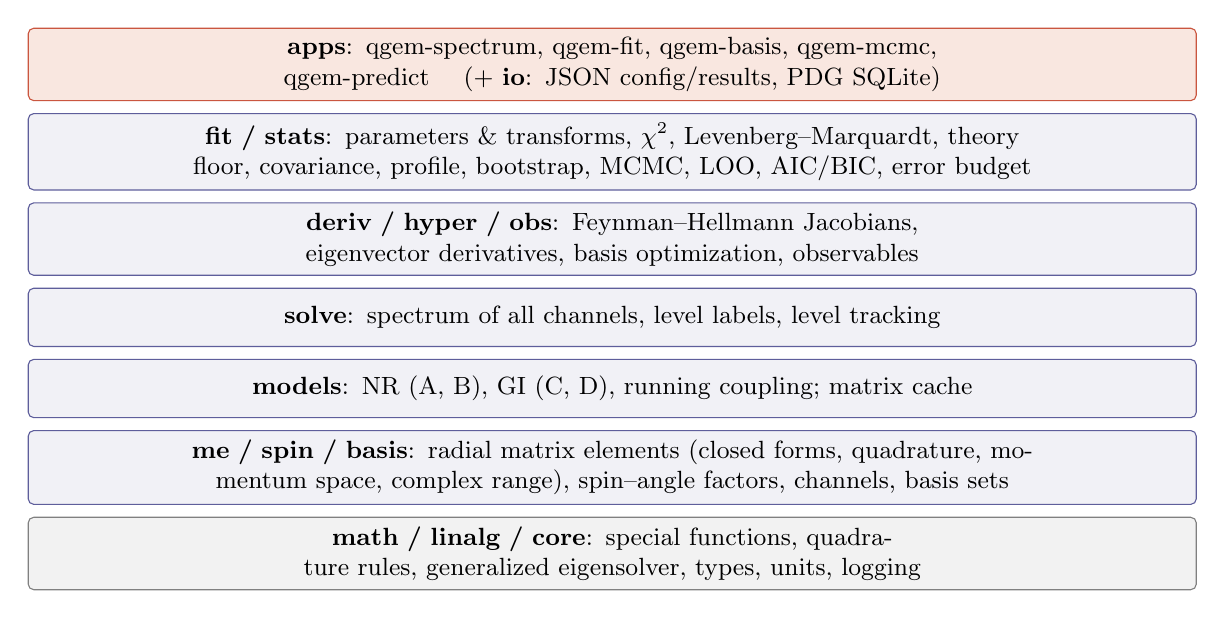
\begin{tikzpicture}[node distance=1.5mm, box/.style={draw=MidnightBlue!70,fill=MidnightBlue!6,rounded corners=2pt,text width=14.6cm,minimum height=7.4mm,align=center,font=\small}]
\node[box,fill=BrickRed!8,draw=BrickRed!70] (apps) {\textbf{apps}: \code{qgem-spectrum}, \code{qgem-fit}, \code{qgem-basis}, \code{qgem-mcmc}, \code{qgem-predict} \quad (+ \textbf{io}: JSON config/results, PDG SQLite)};
\node[box,below=of apps] (stats) {\textbf{fit / stats}: parameters \& transforms, $\chi^2$, Levenberg--Marquardt, theory floor, covariance, profile, bootstrap, MCMC, LOO, AIC/BIC, error budget};
\node[box,below=of stats] (deriv) {\textbf{deriv / hyper / obs}: Feynman--Hellmann Jacobians, eigenvector derivatives, basis optimization, observables};
\node[box,below=of deriv] (solve) {\textbf{solve}: spectrum of all channels, level labels, level tracking};
\node[box,below=of solve] (models) {\textbf{models}: NR (A, B), GI (C, D), running coupling; matrix cache};
\node[box,below=of models] (me) {\textbf{me / spin / basis}: radial matrix elements (closed forms, quadrature, momentum space, complex range), spin--angle factors, channels, basis sets};
\node[box,below=of me,fill=black!5,draw=black!50] (math) {\textbf{math / linalg / core}: special functions, quadrature rules, generalized eigensolver, types, units, logging};
\end{tikzpicture}
\caption{Layers of the program. Arrows are implicit: every layer calls only the layers below it.}\label{fig:bp-layers}
\end{figure}

\paragraph{One $\chi^2$ evaluation, end to end.} (i) The fitter hands an unconstrained vector $\bm u$ to the parameter layer, which maps it to physical $\vth$ (exponentials for positive parameters, \S\ref{sec:minimize}). (ii) For every channel needed by the data, the model assembles $\mH(\vth)$ from cached parameter-independent matrices and the few matrices that depend non-linearly on a parameter (Algorithm~\ref{alg:assembleNR}). (iii) The solver diagonalizes (Algorithm~\ref{alg:gep}) and labels the levels. (iv) The data layer picks the predicted masses (or splittings, widths) and forms whitened residuals $z_i$. (v) If a Jacobian is requested, the derivative layer returns $\partial z_i/\partial u_a$ by Feynman--Hellmann (Algorithm~\ref{alg:fh}). Steps (ii)--(iii) cost $\approx0.3\,$ms for Model~A with four channels of 30 functions (measured).

% ---------------------------------------------------------------------
\subsection{Toolchain and libraries}\label{sec:bp-libs}
\begin{center}\small
\renewcommand{\arraystretch}{1.15}
\begin{tabular}{@{}p{2.7cm}p{2.2cm}p{5.3cm}p{4.3cm}@{}}\toprule
component & on your machine & used for & CMake target / note\\\midrule
GCC & 16.2.1 & C++26 compiler (\code{std::expected}, \code{std::span}, \code{std::numbers}, special math) & needs CMake $\ge3.30$ for \code{CXX_STANDARD 26}\\
CMake & 4.4.4 & build & \code{cmake_minimum_required(VERSION 3.30)}\\
Eigen & \textbf{5.0.1} & dense linear algebra, eigensolvers & \code{Eigen3::Eigen}; \emph{no version} in \code{find_package} (see below)\\
spdlog / fmt & 1.17 / 12.2 & logging, formatting & \code{spdlog::spdlog}\\
SQLite & 3.53 & PDG database & \code{SQLite3::SQLite3} (CMake $\ge4.1$; \code{SQLite::SQLite3} is deprecated)\\
GoogleTest & 1.18 & unit tests & \code{GTest::gtest_main}\\
Ceres Solver & 2.2.0 & optional: LM with bounds, covariance & \code{Ceres::ceres}\\
nlohmann-json & \emph{not installed} & configuration, results, golden files & \code{nlohmann_json::nlohmann_json}; install with \code{pacman -S nlohmann-json}\\
Python 3 + numpy, matplotlib & --- & plots, comparison with your \code{gem_solver.py} & outside the C++ build\\\bottomrule
\end{tabular}
\end{center}
\begin{itemize}[leftmargin=1.3em,itemsep=2pt]
\item \emph{Eigen version.} Your README says Eigen~3.4, but the installed version is 5.0.1. The calls used here (\code{SelfAdjointEigenSolver}, \code{GeneralizedSelfAdjointEigenSolver}, \code{LLT}, \code{LDLT}) behave identically in both (verified with 3.4.0 and 5.0.1). However \code{find_package(Eigen3 3.4 NO_MODULE)} \emph{fails} with 5.0.1 (verified): the version check rejects a different major version. Write \code{find_package(Eigen3 REQUIRED NO_MODULE)} and update the README.
\item \emph{No Boost needed.} Everything special is either in \code{<cmath>} (\code{std::tgamma}, \code{std::lgamma}, \code{std::erf}, \code{std::erfc}; and in libstdc++ \code{std::sph_bessel}, verified) or short enough to write and test yourself: $\erfcx$ (\S\ref{sec:bp-verified}), Gauss--Legendre and generalized Gauss--Laguerre rules by the Golub--Welsch method (Algorithm~\ref{alg:gw}). Note that clang's libc++ does not provide most C++17 special functions; on Linux clang uses libstdc++ by default, so this only matters if you switch standard libraries (not tested).
\item \emph{Optimizer.} Write your own Levenberg--Marquardt (Algorithm~\ref{alg:lm}, $\sim$100 lines with Eigen); the harness version reproduces the worked fit. Ceres is a good cross-check and gives bounds and covariances for free; a verified minimal use with an analytic Jacobian is in \S\ref{sec:bp-verified}. Ceres minimizes $\frac12\sum r_i^2$, so $\chi^2=2\times$\code{final_cost}. NLopt (derivative-free and global optimizers) is not installed and not needed: basis optimization uses Nelder--Mead or the Feynman--Hellmann gradient, and the global stage of a physics fit uses multistart.
\item \emph{SIMD.} \code{std::simd} is not needed (Eigen vectorizes its kernels). For the record: \code{<simd>} with \code{std::simd::vec<float>} compiles with GCC~16.2 and \code{-std=c++26} on your machine.
\item \emph{Random numbers.} Use \code{std::mt19937_64} with an explicit seed; its output sequence is fixed by the standard. The \emph{distributions} (\code{std::normal_distribution}, \dots) are not: their algorithms are implementation-defined, so the same seed can give different Gaussian samples with another standard library. For bit-reproducible bootstrap/MCMC across compilers, generate Gaussians yourself from the engine (Box--Muller), or record the compiler with the results.
\end{itemize}

% ---------------------------------------------------------------------
\subsection{Repository layout and build}\label{sec:bp-layout}
\begin{lstlisting}[style=plain]
Quarkonium-System/
  CMakeLists.txt
  config/        run configurations (JSON): model, parameters, basis, data, seeds
  data/          pdg-2026.0.sqlite (gitignored)
  src/           every name below is a .hpp/.cpp pair unless marked
    core/        types (.hpp)  constants (.hpp)  log  error
    math/        special  quadrature
    linalg/      gep                          <- grows out of your linalg.{hpp,cpp}
    basis/       basis
    me/          radial  smeared  momentum  complex_range  gi
    spin/        channels  factors
    models/      model (.hpp)  nr_model  gi_model  alpha_s  cache
    solve/       spectrum                     <- grows out of your gem_solver.{hpp,cpp}
    obs/         observables  angular (6j, C_fi)
    deriv/       derivatives
    hyper/       basis_opt
    data/        pdg  dataset  assignment
    fit/         params  chi2  lm  floor  uncertainty  multistart
    stats/       bootstrap  mcmc  diagnostics  loo  compare
    report/      budget  json_io
    apps/        qgem_spectrum  qgem_fit  qgem_basis  qgem_mcmc  qgem_predict  (.cpp)
    generated/   qgem_kernels.hpp             <- written by the generator, committed ((*@\S\ref{sec:mma-gen}@*))
  tests/         test_*.cpp (GoogleTest), golden/*.json
                 test_generated_kernels.cpp   <- written by the generator, committed
  python/        plot_spectrum.py  plot_corner.py  compare_golden.py
  mathematica/   QGEMEngine.wl  generate_kernels.wls  QGEMKernels.cmake
                 derivations/D01..D07  (evaluated notebooks, (*@\S\ref{sec:mma-gen}@*))
                 your own notebooks, golden-value generators ((*@\S\ref{sec:mathematica}@*))
  docs/
\end{lstlisting}
Build the code once as a static library \code{qgem} and link the apps and the tests against it. A minimal \code{CMakeLists.txt} (CMake~4.4.4, GCC~16.2.1, Eigen~5.0.1, GoogleTest on your machine):
\begin{lstlisting}[style=cmake]
cmake_minimum_required(VERSION 3.30)   # CXX_STANDARD 26 with GCC needs >= 3.30
project(QuarkoniumGEM VERSION 0.1 LANGUAGES CXX)
include(mathematica/QGEMKernels.cmake)   # option to regenerate the Mathematica-derived kernels
set(CMAKE_CXX_STANDARD 26)
set(CMAKE_CXX_STANDARD_REQUIRED ON)
set(CMAKE_CXX_EXTENSIONS OFF)
set(CMAKE_EXPORT_COMPILE_COMMANDS ON)  # for clangd / clang-tidy
if(NOT CMAKE_BUILD_TYPE)
  set(CMAKE_BUILD_TYPE Release)
endif()

find_package(Eigen3 REQUIRED NO_MODULE)   # no version: accepts 3.4 and 5.x
find_package(spdlog REQUIRED)
find_package(SQLite3 REQUIRED)            # target SQLite3::SQLite3 needs CMake >= 4.1
find_package(nlohmann_json 3.11 REQUIRED)
find_package(Ceres QUIET)                 # optional cross-check
find_package(GTest REQUIRED)

add_compile_options(-Wall -Wextra -Wpedantic)

file(GLOB_RECURSE QGEM_SOURCES CONFIGURE_DEPENDS src/*.cpp)
list(FILTER QGEM_SOURCES EXCLUDE REGEX "src/apps/")
add_library(qgem STATIC ${QGEM_SOURCES})
target_include_directories(qgem PUBLIC src)
target_link_libraries(qgem PUBLIC Eigen3::Eigen spdlog::spdlog SQLite3::SQLite3
                                  nlohmann_json::nlohmann_json)

foreach(app qgem_spectrum qgem_fit qgem_basis qgem_mcmc qgem_predict)
  add_executable(${app} src/apps/${app}.cpp)
  target_link_libraries(${app} PRIVATE qgem)
endforeach()

enable_testing()
file(GLOB TEST_SOURCES CONFIGURE_DEPENDS tests/test_*.cpp)
add_executable(qgem_tests ${TEST_SOURCES})
target_link_libraries(qgem_tests PRIVATE qgem GTest::gtest_main)
qgem_use_generated_kernels(qgem qgem_tests)   # no-op unless QGEM_REGENERATE_KERNELS=ON
include(GoogleTest)
gtest_discover_tests(qgem_tests)
\end{lstlisting}
(This file was verified on your machine exactly as printed, with a dummy source tree of one library file, the five apps and a test, except for the two \code{nlohmann_json} lines, which had to be removed because the package is not installed there yet: it configured without warnings, built, and \code{ctest} passed. It was verified again with the two lines for the generated kernels and the generated header and tests in place: 37 tests passed.) Build with \code{cmake -S . -B build && cmake --build build -j && ctest --test-dir build}. Your existing CI job runs \code{clang-format}; add a second job that builds and runs \code{ctest}.

% ---------------------------------------------------------------------
\subsection{Conventions}\label{sec:bp-conv}
\begin{itemize}[leftmargin=1.3em,itemsep=2pt]
\item \emph{Units}: GeV and GeV$^{-1}$ everywhere inside the program, $\hbar=c=1$. Drop the \code{hbar} member of \code{QuarkoniumSystem}; keep one constant $\hbar c=0.1973269804\GeV\fm$ for printing radii in fm. Masses read from the PDG file are in MeV: convert once, at the boundary.
\item \emph{Types}: \code{Mat = Eigen::MatrixXd}, \code{Vec = Eigen::VectorXd}, \code{CMat = Eigen::MatrixXcd}. Replace \code{std::vector<std::vector<double>>}: it is an array of separately allocated rows, so matrix products cannot be vectorized and every access is a double indirection.
\item \emph{Naming}: one name per mathematical object, matching the notes (\code{S}, \code{H}, \code{nu}, \code{mr}, \code{kappa}, \code{sigma_th}). Functions that return matrices are nouns (\code{overlap}, \code{kinetic_nr}); functions that do work are verbs (\code{solve_gep}, \code{fit}).
\item \emph{Errors}: throw for programming and configuration errors (unknown channel, missing PDG entry). Return \code{std::expected<T, Error>} for \emph{numerical} failures that a caller may want to survive (a parameter point where the overlap has no eigenvalue above $\eta$, a collapsing Hamiltonian): the fitter turns them into $\chi^2=+\infty$ and shrinks the step. Your current code throws in that case, which would abort a fit.
\item \emph{Logging}: \code{spdlog} at \code{info} for run-level events, \code{debug} for per-iteration details, \code{warn} for anything that changes results silently (levels dropped by $\eta$, a level-tracking swap, a parameter at a bound).
\item \emph{Determinism}: every stochastic routine takes a seed; parallel code gives each thread its own engine seeded from (master seed, thread index).
\end{itemize}

% ---------------------------------------------------------------------
\subsection{From your current code to the new layout}\label{sec:bp-migrate}
Your \code{gem_solver.cpp} already contains the core of Models A/B for one channel. The following changes turn it into the \code{models}/\code{solve} layers; keep the current version and its golden test until the new one reproduces it.
\begin{enumerate}[leftmargin=1.5em,itemsep=2pt]
\item \emph{Normalized closed forms.} You compute un-normalized integrals with \code{std::tgamma} and \code{std::pow} and divide by the norms at the end. For large $l$ or extreme ranges the intermediate numbers over- or underflow. Use the normalized forms: $S_{ij}=\big(2\sqrt{\nu_i\nu_j}/(\nu_i+\nu_j)\big)^{l+3/2}$, $\langle r^k\rangle_{ij}=S_{ij}\,\frac{\Gamma(l+\frac{k+3}2)}{\Gamma(l+\frac32)}(\nu_i+\nu_j)^{-k/2}$, $T_{ij}=\frac{2l+3}{\mr}\frac{\nu_i\nu_j}{\nu_i+\nu_j}S_{ij}$, with \code{std::lgamma} for the gamma ratio (verified to reproduce Tests 1--2).
\item \emph{Solver.} The LLT path with a $10^{-12}$ diagonal jitter on failure silently changes the problem. Use canonical orthogonalization (Algorithm~\ref{alg:gep}) as the default and log the number of kept directions; keep the Cholesky path as \code{solve_gep_cholesky} for cross-checks.
\item \emph{Spin.} Replace \code{int spin} with a \code{Channel}; replace the hard-coded $-\frac34,\frac14$ by \code{s1s2(S)} and add the spin--orbit, tensor and ${}^1L_L$--${}^3L_L$ factors (\S\ref{sec:bp-catalogue}).
\item \emph{Hyperfine in $P$ waves.} Your code includes the smeared contact term for $l=0$ only. With smearing it has small but non-zero $P$-wave matrix elements (\S\ref{sec:me}); the worked example includes it in every channel. Either choice is a model choice: make it a configuration flag and state which one you use.
\item \emph{Smearing default.} \code{sigma_smear} defaults to $\sqrt{\mr}$ (a legacy of the Python code). Make $\sigma$ an explicit parameter with no hidden default.
\item \emph{Matrix cache.} Build $\mS$, $\mathbf T/\mr$ (as $\mathbf T_1$ with $\mr=1$), $\langle r^{-1}\rangle$, $\langle r\rangle$ once per basis; only $\langle\delta_\sigma\rangle$ depends non-linearly on a parameter. This is what makes a model evaluation cost $0.3\,$ms.
\end{enumerate}

% ---------------------------------------------------------------------
\subsection{Core data structures}\label{sec:bp-types}
\begin{lstlisting}[style=cpp]
namespace qgem {
using Mat = Eigen::MatrixXd;   using Vec = Eigen::VectorXd;
using CMat = Eigen::MatrixXcd; using cplx = std::complex<double>;
inline constexpr double hbarc = 0.1973269804;   // GeV fm, output only

// ---- spin/channels.hpp
struct Component { int L, S; };                  // one partial wave (L, S)
struct Channel {                                 // one block  H c = E S c
  int J, P, C;                                   // J^{PC}; C = 0 if m1 != m2
  std::vector<Component> comps;                  // 1, or 2 if coupled
  std::string label() const;                     // "3S1-3D1", "1P1", "3P0", ...
};

// ---- basis/basis.hpp
struct BasisSpec {                               // per partial wave L
  int n = 30;  double r1 = 0.02, rmax = 30.0;    // real-range set (GeV^-1)
  int nc = 0;  double rho1 = 1.0, rhomax = 20.0, omega = 0.5;   // complex-range set
  double eta = 1e-12;                            // orthogonalization threshold
};
enum class Fn { Real, Cos, Sin };
struct Basis { int L = 0; std::vector<cplx> z; std::vector<Fn> kind; Vec norm; };

// ---- fit/params.hpp
enum class Transform { Identity, Log, OrderedLog };   // OrderedLog: gamma_1 < gamma_2 < ...
struct ParamSpec {
  std::string name;  double value;  bool free = true;
  Transform tr = Transform::Identity;
  double lo = -INFINITY, hi = INFINITY;
  std::optional<std::pair<double, double>> prior;  // Gaussian (mean, sigma) -> penalty
};
class ParamSet {                                 // free, transformed u <-> physical theta
 public:
  Vec theta(const Vec& u) const;  Vec u(const Vec& theta) const;
  Mat dtheta_du(const Vec& u) const;             // diagonal except for OrderedLog
  int n_free() const;  std::span<const ParamSpec> specs() const;
};

// ---- solve/spectrum.hpp
struct StateId { std::string channel; int n; };  // {"3P0", 0} = lowest 3P0 level
struct Level {
  Channel ch;  int n;  double E, M;              // M = E + mass offset
  Vec c;                                         // c^T S c = 1
  std::vector<double> prob;                      // component probabilities
};
struct Spectrum {
  std::vector<Level> levels;
  const Level& at(const StateId&) const;
};

// ---- data/dataset.hpp
struct Datum {
  std::string label;  long mcid = 0;             // PDG Monte Carlo id
  enum class Kind { Mass, Splitting, Width, Ratio } kind = Kind::Mass;
  std::vector<StateId> states;                   // mass: 1 state; splitting: 2
  double y = 0, err_plus = 0, err_minus = 0;     // GeV
  std::string sys_group;  double sys_common = 0; // common systematic ((*@Ex.~\ref{ex:chib}@*))
  bool in_fit = true;  double extra_floor = 0;   // e.g. states above threshold
};
struct Dataset {
  std::vector<Datum> d;
  Mat V_exp() const;                             // incl. common systematics
};

// ---- fit/fit.hpp
struct FitOptions {
  double lambda0 = 1e-3;  int max_iter = 200;  double ftol = 1e-12, xtol = 1e-10;
};
struct FitResult {
  Vec u, theta;  double chi2 = 0;  int ndof = 0;  double sigma_th = 0;
  Mat Jz;                                        // whitened Jacobian dz/du (N x p)
  Mat C;                                         // covariance of theta
  Vec residuals, pulls, leverage;
  int iterations = 0;  bool converged = false;
};
}  // namespace qgem
\end{lstlisting}

\paragraph{The model interface.} Models differ only in how they assemble $\mH$; everything else is shared.
\begin{lstlisting}[style=cpp]
struct ChannelMatrices { Mat H, S; bool orthonormal = false; };  // GI builds H' directly

// Parameter-independent matrices per (channel, basis). An entry that depends on one
// non-linear parameter (sigma, mu_s, tau_k) stores that value and is rebuilt when it changes.
class MatrixCache;

class Model {
 public:
  virtual ~Model() = default;
  virtual std::string name() const = 0;
  virtual ParamSet parameters() const = 0;
  virtual double mass_offset(const Vec& theta) const = 0;   // m1+m2 (A, B) or 0 (C, D)
  virtual ChannelMatrices build(const Channel&, const Vec& theta, MatrixCache&) const = 0;
  // dH/dtheta_a for all parameters; default implementation: central differences of build()
  virtual std::vector<Mat> dH(const Channel&, const Vec& theta, MatrixCache&) const;
};
class NRModel final : public Model { /* Models A and B: flags screened, spin_mode */ };
class GIModel final : public Model { /* Models C and D: flag screened, alpha_s form */ };
std::unique_ptr<Model> make_model(const nlohmann::json& config);
\end{lstlisting}

% ---------------------------------------------------------------------
\subsection{Function catalogue}\label{sec:bp-catalogue}
Signatures with their contracts as comments. Every matrix function returns a matrix in the normalized basis.

\subsubsection*{math/special, math/quadrature}
\begin{lstlisting}[style=cpp]
// Int_0^inf r^p e^{-a r^2} dr = Gamma((p+1)/2) / (2 a^{(p+1)/2}), evaluated with lgamma
double master_integral(double p, double a);
cplx   master_integral(double p, cplx a);        // principal branch, Re a > 0 (complex range)
double erfcx(double x);                          // e^{x^2} erfc x ((*@\S\ref{sec:bp-verified}@*))
// I_j(a, tau), j = 0..jmax, and Q_k(a, mu), k = 0..kmax: the recursions of (*@\S\ref{sec:me}@*)
void   erf_t_integrals(int jmax, double a, double tau, std::span<double> I);
// Q_k: upward for x = mu/(2 sqrt a) < 1/2, downward ratios otherwise (the remark after the Q_k lemma);
// the generated header has this function as gen::detail::screened_moments
void   screened_moments(int kmax, double a, double mu, std::span<double> Q);
// smeared r and e^{-mu r} with their r-derivatives: eqs. (*@\eqref{eq:smlin}, \eqref{eq:smexp}@*), erfcx form
double smeared_r(double r, double s);              double smeared_r_d(double r, double s);
double smeared_exp(double r, double mu, double s);  double smeared_exp_d(double r, double mu, double s);
double gi_alpha_s(double Q, std::span<const double> alpha, std::span<const double> gamma);
struct QuadRule { Vec x, w; };
const QuadRule& gauss_legendre01(int n);           // cached rule on [0, 1]
const QuadRule& gauss_laguerre(int n, double alpha);  // cached, weight t^alpha e^{-t} on [0, inf)
\end{lstlisting}

\subsubsection*{linalg, basis}
\begin{lstlisting}[style=cpp]
struct GepResult { Vec E; Mat C; Mat X; int n_kept; double s_min, s_max; };
Mat       orthonormalizer(const Mat& S, double eta);   // X with X^T S X = 1, kept directions
GepResult solve_gep(const Mat& H, const Mat& S, double eta = 1e-12);   // (*@Alg.~\ref{alg:gep}@*)
GepResult solve_gep_cholesky(const Mat& H, const Mat& S);  // your current method, cross-checks
Basis  make_basis(int L, const BasisSpec&);              // (*@Alg.~\ref{alg:basis}@*)
Basis  nested_double(const Basis&);                      // n -> 2n-1: every old function kept
double radial_value(const Basis&, const Vec& c, double r);
Vec    origin_coefficients(const Basis&);   // v_n = N_nL: R(0) = c.v (L=0), R ~ (c.v) r^L
\end{lstlisting}

\subsubsection*{me (radial matrix elements)}
\code{bra} and \code{ket} bases may have different $L$ (tensor coupling, transitions). The closed forms for one pair of basis functions, with their parameter derivatives, are in the generated header \code{generated/qgem_kernels.hpp} (\S\ref{sec:mma-gen}): \code{qgem::gen::overlap}, \code{kinetic}, \code{r_power}, \code{gaussian}, \code{erf_over_r}, \code{screened_exp}, \code{smeared_linear}, \code{smeared_exp}, their spin--orbit and tensor partners, and the complex-range bilinear forms. The functions below fill matrices from them; write them yourself or use the generated ones, and test one against the other.
\begin{lstlisting}[style=cpp]
Mat overlap(const Basis&);
Mat kinetic_nr(const Basis&, double mr);                          // T = p^2/(2 mr)
Mat r_power(const Basis& bra, const Basis& ket, double k);        // <r^k>, L+L'+3+k > 0
Mat gaussian(const Basis& bra, const Basis& ket, double beta);   // <e^{-beta r^2}>
Mat erf_over_r(const Basis&, double tau);                         // <erf(tau r)/r>
Mat exp_power(const Basis&, double mu, int k);                    // <r^k e^{-mu r}>
// any V(r): Gauss-Legendre on [0, sqrt(40/a)] per pair, cached rule rescaled
Mat local(const Basis& bra, const Basis& ket, const std::function<double(double)>& V,
          int nq = 128);
// <f(p)>: generalized Gauss-Laguerre with alpha = L + 1/2
Mat momentum_diagonal(const Basis&, const std::function<double(double)>& f, int nq = 64);

// ---- me/gi.hpp: tilde G, tilde S and the GI spin radial functions
struct GILocal { Mat G, Sconf, contact, tensor, so_v, so_s; };
GILocal gi_local(const Basis& bra, const Basis& ket, const GIParams&, bool screened);
// closure: returns (Xb^T Fb Xb)(Xb^T W Xk)(Xk^T Fk Xk), i.e. F'W'F' in orthonormal bases
Mat sandwich_closure(const Mat& Fbra, const Mat& W, const Mat& Fket,
                     const Mat& Xbra, const Mat& Xket);
// two-step: tabulate chi_n = f(p) R_n on radial nodes, then integrate chi W chi
Mat sandwich_two_step(const Basis&, const std::function<double(double)>& f,
                      const std::function<double(double)>& W, int np, int nr);
\end{lstlisting}

\subsubsection*{spin}
Values verified symbolically (\S\ref{sec:mma-spin}).
\begin{lstlisting}[style=cpp]
double s1s2(int S);              // -3/4 (S=0), +1/4 (S=1)
double ls(int L, int S, int J);  // [J(J+1) - L(L+1) - S(S+1)]/2
// S=1 only; L=0 gives 0. J=L+1: -2L/(2L+3);  J=L: 2;  J=L-1: -2(L+1)/(2L-1)
double s12_diag(int L, int J);
double s12_offdiag(int J);       // <(J-1)1J|S12|(J+1)1J> = 6 sqrt(J(J+1))/(2J+1); 3S1-3D1: 2 sqrt 2
double ls_minus(int L);          // <1L_L| L.(S1-S2) |3L_L> = sqrt(L(L+1)), m1 != m2 only
std::vector<Channel> enumerate_channels(int Lmax, bool equal_masses);
\end{lstlisting}

\subsubsection*{models, solve, obs}
\begin{lstlisting}[style=cpp]
Spectrum solve_spectrum(const Model&, const Vec& theta, std::span<const Channel>,
                        MatrixCache&);
// new level b for every old level a: argmax_b |c_b(new)^T S c_a(old)|
std::vector<int> track_levels(const Mat& S, const Mat& C_old, const Mat& C_new);
double R0_squared(const Level&, const Basis&);              // |R(0)|^2, S waves
double origin_derivative(const Level&, const Basis&);       // R'(0) (P), R''(0) (D) via A_L
double moment(const Level&, const Basis&, double k);        // <r^k>
double radial_overlap(const Level& f, const Level& i, double k);  // <f|r^k|i>, L may differ
// widths of (*@\S\ref{sec:observables}@*); E1 uses C_fi from 6j, M1 <j0(kr/2)> by quadrature
double width_ee(const Level&, double M, double eQ, double qcd_factor);
double width_E1(const Level& i, const Level& f, double eQ);
double width_M1(const Level& i, const Level& f, double eQ, double mQ);
double sixj(int j1, int j2, int j3, int j4, int j5, int j6);   // Racah formula
\end{lstlisting}

\subsubsection*{deriv, hyper}
\begin{lstlisting}[style=cpp]
// N x p Jacobian of the predictions by Feynman-Hellmann ((*@Alg.~\ref{alg:fh}@*))
Mat jacobian_fh(const Model&, const Vec& theta, const Spectrum&, const Dataset&,
                MatrixCache&);
Vec eigvec_derivative(const GepResult&, int a, const Mat& dH, const Mat& dS);  // (*@\eqref{eq:dvec}@*)
Mat jacobian_fd(const std::function<Vec(const Vec&)>& f, const Vec& x, const Vec& h);
struct HyperResult { BasisSpec spec; double objective; std::vector<double> nested_shift; };
HyperResult optimize_basis(const Model&, const Vec& theta0, const Channel&,
                           BasisSpec start, int K, std::span<const double> weights);  // (*@Alg.~\ref{alg:hyper}@*)
double numerical_error(const Model&, const Vec& theta, const Channel&, const BasisSpec&,
                       const StateId&);
\end{lstlisting}

\subsubsection*{data, fit, stats, report}
\begin{lstlisting}[style=cpp]
class PdgDatabase;                                // (*@\S\ref{sec:bp-data}@*) (verified)
Dataset load_dataset(const nlohmann::json& selection, const PdgDatabase&);
double  open_flavour_threshold(const PdgDatabase&, char flavour);  // 2 M(D0) or 2 M(B0)

class Chi2Problem {                               // model + data + parameters + floor
 public:
  Chi2Problem(const Model&, Dataset, ParamSet, double sigma_th);
  std::expected<Vec, Error> residuals(const Vec& u);   // whitened z_i
  std::expected<Mat, Error> jacobian(const Vec& u);    // dz/du (Feynman-Hellmann or FD)
  void set_sigma_th(double);  int n_data() const;  int n_free() const;
};
FitResult levenberg_marquardt(Chi2Problem&, Vec u0, const FitOptions&);   // (*@Alg.~\ref{alg:lm}@*)
double    solve_theory_floor(const Vec& Delta, const Vec& s_exp, int nu); // (*@Alg.~\ref{alg:floor}@*)
FitResult fit_with_floor(Chi2Problem&, Vec u0, const FitOptions&);
FitResult multistart(Chi2Problem&, int n_starts, std::uint64_t seed);

struct Uncertainty {
  Mat C, rho;  Vec sigma, sigma_conditional, fisher_eigenvalues;  Mat fisher_eigenvectors;
};
Uncertainty analyse(const FitResult&);                                    // (*@Alg.~\ref{alg:unc}@*)
std::vector<std::pair<double, double>> profile(Chi2Problem&, const FitResult&, int a,
                                               std::span<const double> grid);
struct Samples { Mat theta; Vec chi2; double acceptance = 0; };
Samples parametric_bootstrap(Chi2Problem&, const FitResult&, int B,
                             std::uint64_t seed);                         // (*@Alg.~\ref{alg:boot}@*)
std::vector<Samples> metropolis(Chi2Problem&, const FitResult&, int chains, int steps,
                                int burn, std::uint64_t seed);            // (*@Alg.~\ref{alg:mcmc}@*)
Vec rhat(std::span<const Samples>);
Vec tau_int(const Samples&);
struct LooResult { Vec leverage, loo_residual, pull; };
LooResult leave_one_out(Chi2Problem&, const FitResult&, bool exact_refits);
double aic(const FitResult&);
double bic(const FitResult&);
struct Budget { double value, par, num, th, amb, model_spread; };
// arguments: prediction functor, fit, basis variants, convention variants  ((*@Alg.~\ref{alg:budget}@*))
Budget error_budget(/* ... */);
void   write_json(const std::string& path, const nlohmann::json&);
\end{lstlisting}

% ---------------------------------------------------------------------
\subsection{Algorithms}\label{sec:bp-alg}
Notation as in \S\ref{sec:gem}--\S\ref{sec:stats}. Line comments ($\triangleright$) give the reason for each step.

\begin{algorithm}[H]
\caption{Build a basis for one partial wave $L$}\label{alg:basis}
\begin{algorithmic}[1]
\Require $L$; real set $(n,r_1,r_{\max})$; complex set $(n_c,\rho_1,\rho_{\max},\omega)$
\State $q\gets(r_{\max}/r_1)^{1/(n-1)}$
\For{$k=0,\dots,n-1$} \State append $z=1/(r_1q^k)^2$, kind \textsc{Real} \EndFor
\If{$n_c>0$}
  \State $q_c\gets(\rho_{\max}/\rho_1)^{1/(n_c-1)}$
  \For{$k=0,\dots,n_c-1$} \State $\eta_k\gets1/(\rho_1q_c^k)^2$; append $(\eta_k(1+\ii\omega),\textsc{Cos})$ and $(\eta_k(1+\ii\omega),\textsc{Sin})$ \EndFor
\EndIf
\For{each function $i$} \Comment{normalize so that $S_{ii}=1$}
  \State compute the unnormalized $S_{ii}$ from the master integral (real) or the rules \eqref{eq:cs} (cos/sin); $\text{norm}_i\gets S_{ii}^{-1/2}$
\EndFor
\Ensure \code{Basis}; real functions alone have the closed form $N_{nL}$ of \S\ref{sec:basis}
\end{algorithmic}
\end{algorithm}

\begin{algorithm}[H]
\caption{Gauss quadrature by Golub--Welsch (Legendre, generalized Laguerre)}\label{alg:gw}
\begin{algorithmic}[1]
\Require $n$; for Laguerre the exponent $\alpha$ of the weight $t^\alpha\ee^{-t}$
\State build the symmetric tridiagonal Jacobi matrix $\mathsf T$:
\Statex \hspace{1.5em} Legendre: $\mathsf T_{kk}=0$, $\mathsf T_{k,k-1}=k/\sqrt{4k^2-1}$, $\mu_0=2$ \Comment{on $[-1,1]$}
\Statex \hspace{1.5em} Laguerre: $\mathsf T_{kk}=2k+\alpha+1$, $\mathsf T_{k,k-1}=\sqrt{k(k+\alpha)}$, $\mu_0=\Gamma(\alpha+1)$
\State diagonalize $\mathsf T=\mathbf V\diag(x_i)\mathbf V^T$ \Comment{\code{SelfAdjointEigenSolver}}
\State nodes $x_i$; weights $w_i\gets\mu_0\,V_{0i}^2$ \Comment{first component of each eigenvector}
\State cache the rule by $(n,\alpha)$ \Comment{rebuilding it per matrix element costs $10^3\times$}
\Ensure $\sum_iw_ix_i^k=\Gamma(\alpha+k+1)$ for $k\le2n-1$ (unit test)
\end{algorithmic}
\end{algorithm}

\begin{algorithm}[H]
\caption{Assemble one channel of Model A/B}\label{alg:assembleNR}
\begin{algorithmic}[1]
\Require channel with components $\alpha=(L_\alpha,S)$; parameters $\vth=(m_1,m_2,\as,b,c,\sigma[,\mus])$; cache
\For{each component $\alpha$}
  \State fetch from cache (built once per basis): $\mS$, $\mathbf T_1$ ($\mr=1$), $\langle r^{-1}\rangle$, $\langle r\rangle$, $\langle r^{-3}\rangle$ ($L\ge1$)
  \State fetch or rebuild if $\sigma$ changed: $\mathbf G_\sigma=\langle\ee^{-\sigma^2r^2}\rangle$; if $\mus$ changed: $\langle\ee^{-\mus r}\rangle$, $\langle\ee^{-\mus r}/r\rangle$
  \State $\mH_{\alpha\alpha}\gets\mathbf T_1/\mr+c\,\mS-\tfrac43\as\langle r^{-1}\rangle+V_S+\tfrac{32\pi\as}{9m_1m_2}\big(\tfrac{\sigma}{\sqrt\pi}\big)^3\mathtt{s1s2}(S)\,\mathbf G_\sigma$
  \Statex \hspace{1.5em}with $V_S=b\langle r\rangle$ (A) or $\frac b{\mus}(\mS-\langle\ee^{-\mus r}\rangle)$ (B)
  \If{spin--orbit/tensor non-perturbative (smeared versions only, \S\ref{sec:modelA})} add $o_k(L,S,J)\,\mathbf W_k$ \EndIf
\EndFor
\If{two components} \Comment{tensor $L=J\mp1$, or ${}^1L_L$--${}^3L_L$ for $m_1\ne m_2$}
  \State off-diagonal block: \code{s12_offdiag}$(J)\cdot\langle R_{L_1}|W_T|R_{L_2}\rangle$, or \code{ls_minus}$(L)\cdot\langle B(r)\rangle$
\EndIf
\State $\mS\gets$ block-diagonal; $\mH\gets\frac12(\mH+\mH^T)$
\Ensure \code{ChannelMatrices}; mass offset $m_1+m_2$ added after diagonalization
\end{algorithmic}
\end{algorithm}
\emph{Perturbative spin terms} (as in the worked example): diagonalize the spin-independent (plus smeared contact) Hamiltonian, then add $\langle\vL\cdot\vS\rangle a+\langle S_{12}\rangle t$ with $a,t$ from the eigenvector; their parameter derivatives need \eqref{eq:dvec}.

\begin{algorithm}[H]
\caption{Assemble one channel of Model C/D (GI) in the orthonormalized basis}\label{alg:assembleGI}
\begin{algorithmic}[1]
\Require channel; $\vth=(m_1,m_2,b,c,\sigma_0,s,\epsilon_c,\epsilon_t,\epsilon_{sov},\epsilon_{sos}[,\{\alpha_k,\gamma_k\}][,\mus])$
\State $\sigma_{12}$ from \eqref{eq:sigma12}; $\tau_k=\gamma_k\sigma_{12}/\sqrt{\gamma_k^2+\sigma_{12}^2}$
\For{each component $L$}
  \State $\mathbf X_L\gets$ \code{orthonormalizer}$(\mS_L,\eta)$ \Comment{cached per basis}
  \State $\mathbf K\gets$ \code{momentum_diagonal}$(E_1+E_2)$; $\mathbf F_G\gets$ \code{momentum_diagonal}$\big((1+p^2/E_1E_2)^{1/2}\big)$
  \State $\bm\Phi_x\gets$ \code{momentum_diagonal}$\big((m_am_b/E_aE_b)^{1/2+\epsilon_x}\big)$ for $x\in\{c,t,sov,sos\}$ \Comment{one $p$-quadrature each}
  \State local matrices $\tilde{\mathbf G}$, $\tilde{\mathbf S}$ (or $\tilde{\mathbf S}_{\rm scr}$), $\mathbf W_c,\mathbf W_t,\mathbf W_{so(v)},\mathbf W_{so(s)}$ \Comment{closed forms or \code{local}}
  \State $\mH'_{LL}\gets\mathbf X^T\mathbf K\mathbf X+\mathbf F'_G\tilde{\mathbf G}'\mathbf F'_G+\tilde{\mathbf S}'+\sum_xo_x(L,S,J)\,\bm\Phi'_x\mathbf W'_x\bm\Phi'_x$ \Comment{$\mathbf A'=\mathbf X^T\mathbf A\mathbf X$}
\EndFor
\State coupled block: $\mH'_{L_1L_2}\gets o_t\,(\mathbf X_1^T\bm\Phi_{t,1}\mathbf X_1)(\mathbf X_1^T\mathbf W_{t,12}\mathbf X_2)(\mathbf X_2^T\bm\Phi_{t,2}\mathbf X_2)$
\State symmetrize; diagonalize $\mH'$ (standard problem); $\mathbf C\gets\mathbf X\mathbf C'$ \Comment{eigenvalues are masses}
\Ensure closure method (ii) of \S\ref{sec:nonlocal}; validate against the two-step method (Test~4)
\end{algorithmic}
\end{algorithm}

\begin{algorithm}[H]
\caption{Generalized eigenproblem by canonical orthogonalization}\label{alg:gep}
\begin{algorithmic}[1]
\Require symmetric $\mH$, positive semi-definite $\mS$ (numerically), threshold $\eta$
\State $\mS=\mathbf U\diag(s_i)\mathbf U^T$, ascending $s_i$ \Comment{\code{SelfAdjointEigenSolver}}
\State keep $\mathcal K=\{i:\ s_i>\eta\,s_{\max}\}$; if $\mathcal K=\varnothing$ return error
\State $\mathbf X\gets\mathbf U_{\mathcal K}\diag(s_i^{-1/2})_{i\in\mathcal K}$ \Comment{$\mathbf X^T\mS\mathbf X=\mathbf 1$}
\State $\mH'\gets\mathbf X^T\mH\mathbf X$; symmetrize; diagonalize $\mH'=\mathbf V\diag(\mathcal E_k)\mathbf V^T$
\State $\mathbf C\gets\mathbf X\mathbf V$ \Comment{columns satisfy $\vc_k^T\mS\vc_k=1$}
\Ensure $\mathcal E$ ascending, $\mathbf C$, $\mathbf X$, $|\mathcal K|$, $s_{\min}/s_{\max}$ (log a warning if $|\mathcal K|<n$)
\end{algorithmic}
\end{algorithm}

\begin{algorithm}[H]
\caption{Label levels and track them between parameter points}\label{alg:track}
\begin{algorithmic}[1]
\Require eigenvectors $\mathbf C^{\rm old}$ (from the previous accepted point), new $\mathbf C$, overlap $\mS$ (unchanged: fixed basis)
\State $\mathbf O\gets|\mathbf C^T\mS\mathbf C^{\rm old}|$ \Comment{$O_{ba}\approx\delta_{ba}$ if nothing crossed}
\For{each old level $a$ that is assigned to a datum}
  \State $b(a)\gets\arg\max_bO_{ba}$; if $b(a)\ne a$ log \code{warn} (level crossing)
\EndFor
\State for coupled channels: label by the dominant component, $P_\alpha=\vc_\alpha^T\mS^\alpha\vc_\alpha$
\Ensure map datum $\to$ level index at the new point
\end{algorithmic}
\end{algorithm}

\begin{algorithm}[H]
\caption{Feynman--Hellmann Jacobian of the whitened residuals}\label{alg:fh}
\begin{algorithmic}[1]
\Require spectrum at $\vth$; for each channel the matrices $\partial\mH/\partial\theta_a$ (\code{Model::dH}); data; transform Jacobian $\partial\vth/\partial\bm u$
\For{each datum $i$ and each parameter $a$}
  \State mass datum with level $(\text{ch},k)$: $\partial\mu_i/\partial\theta_a\gets\vc_k^T(\partial\mH/\partial\theta_a)\vc_k+\partial(\text{offset})/\partial\theta_a$ \Comment{$\mS'=0$}
  \State splitting: difference of two such terms; perturbative add-ons: chain rule with \eqref{eq:dvec}
\EndFor
\State $\partial z_i/\partial\theta_a\gets-(\partial\mu_i/\partial\theta_a)/s_i$; then $\partial z/\partial\bm u=(\partial z/\partial\vth)(\partial\vth/\partial\bm u)$
\Ensure $N\times p$ matrix; unit test against \code{jacobian_fd} (relative agreement $\sim10^{-7}$)
\end{algorithmic}
\end{algorithm}

\begin{algorithm}[H]
\caption{Basis hyperparameter optimization and convergence check}\label{alg:hyper}
\begin{algorithmic}[1]
\Require model at nominal $\vth_0$; channel; start spec; $K$ target levels with weights $w_k>0$
\State variables $\bm\xi=(\ln r_1,\ln r_{\max}[,\ln\rho_1,\ln\rho_{\max},\omega])$; $n$, $n_c$ fixed \Comment{$n$ is not continuous (Property 2)}
\State objective $f(\bm\xi)=\sum_{k<K}w_k\mathcal E_k(\bm\xi)$ \Comment{an upper bound for each $k$ (HUM, Ky Fan)}
\State minimize $f$ with Nelder--Mead, or with the gradient $\partial\mathcal E_k/\partial\xi=\vc_k^T(\mH'-\mathcal E_k\mS')\vc_k$ \eqref{eq:FH}
\State nested check: $n\to2n-1$ (\code{nested_double}); record the shift of every observable as $\sigma_{\rm num}$
\State require $\sigma_{\rm num}\le10^{-2}\min_is_i$; otherwise increase $n$ and repeat
\Ensure frozen \code{BasisSpec} per channel, written to the run configuration
\end{algorithmic}
\end{algorithm}

\begin{algorithm}[H]
\caption{Levenberg--Marquardt on whitened residuals}\label{alg:lm}
\begin{algorithmic}[1]
\Require \code{Chi2Problem}; start $\bm u_0$; $\lambda_0=10^{-3}$; tolerances
\State $\bm z\gets$ residuals$(\bm u)$; $\chi^2\gets\bm z^T\bm z$
\Repeat
  \State $\mathbf J\gets$ jacobian$(\bm u)$; $\sF\gets\mathbf J^T\mathbf J$; $\bm g\gets-\mathbf J^T\bm z$ \Comment{$\mathbf J=\partial\bm z/\partial\bm u$, so $\bm g=\sJ^T\sW\vD$}
  \Loop
    \State solve $(\sF+\lambda\diag\sF)\,\bm\delta=\bm g$ \Comment{\code{ldlt()}}
    \State $\bm z'\gets$ residuals$(\bm u+\bm\delta)$; if it fails (\code{std::expected} error) set $\chi'^2=\infty$
    \If{$\chi'^2<\chi^2$} accept; $\lambda\gets\max(\lambda/10,10^{-12})$; \textbf{break}
    \Else\ $\lambda\gets10\lambda$; if $\lambda>10^{12}$ stop (no progress) \EndIf
  \EndLoop
\Until{$(\chi^2_{\rm old}-\chi^2)/\chi^2<10^{-12}$ and $\max_a|\delta_a|/(|u_a|+10^{-8})<10^{-10}$}
\State covariance in $\bm u$: $(\mathbf J^T\mathbf J)^{-1}$; in $\vth$: $\sC=\mathbf K(\mathbf J^T\mathbf J)^{-1}\mathbf K^T$, $\mathbf K=\partial\vth/\partial\bm u$
\Ensure \code{FitResult}. Bounds: by transforms (log for positive parameters), not by clipping
\end{algorithmic}
\end{algorithm}
Note the sign: with $z_i=(y_i-\mu_i)/s_i$ the Jacobian $\partial z/\partial u$ is minus the whitened $\sJ$, hence $\bm g=-\mathbf J^T\bm z$. Getting this sign wrong makes every step go uphill, and the method then shrinks $\lambda$ forever.

\begin{algorithm}[H]
\caption{Theory floor (common to all states)}\label{alg:floor}
\begin{algorithmic}[1]
\Require start $\sigma_{\rm th}^{(0)}$ (e.g.\ $10\MeV$); $\nu=N-p$
\Repeat
  \State fit with $s_i^2=\sigma_{{\rm exp},i}^2+\sigma_{\rm th}^2$ (Algorithm~\ref{alg:lm}, warm start) $\to$ residuals $\Delta_i$
  \State solve $g(x)=\sum_i\Delta_i^2/(\sigma_{{\rm exp},i}^2+x)-\nu=0$ for $x\ge0$ by bisection on $[0,\sum\Delta_i^2]$ \Comment{$g$ is decreasing}
  \State if $g(0)\le0$ set $x=0$ (no floor needed); $\sigma_{\rm th}\gets\sqrt x$
\Until{$|\Delta\sigma_{\rm th}|<10^{-4}\MeV$} \Comment{2--3 iterations in the worked example}
\Ensure $\sigma_{\rm th}$, final fit with $\chi^2/\nu=1$
\end{algorithmic}
\end{algorithm}

\begin{algorithm}[H]
\caption{Uncertainty analysis at the minimum}\label{alg:unc}
\begin{algorithmic}[1]
\State $\sF\gets\mathbf J^T\mathbf J$ in physical variables; scale $\tilde\sF=\sD_\theta\sF\sD_\theta$ with $\sD_\theta=\diag(\hat\theta_a)$
\State eigen-decompose $\tilde\sF$; condition number $\lambda_{\max}/\lambda_{\min}$; if $>10^{10}$ warn (degenerate direction, print its eigenvector)
\State $\sC\gets\sF^{-1}$ (via the eigen-decomposition); $\sigma_a=\sqrt{\sC_{aa}}$; $\rho_{ab}=\sC_{ab}/(\sigma_a\sigma_b)$
\State conditional errors $1/\sqrt{\sF_{aa}}$ (diagnostic only; never quote them)
\State profile of each key parameter: fix $\theta_a$ on a grid $\hat\theta_a+t\sigma_a$, $t\in[-3,3]$, refit the rest starting from the neighbouring grid point; record $\Delta\chi^2(t)$; interpolate the $\Delta\chi^2=1$ crossings
\Ensure \code{Uncertainty}; flag parameters whose profile deviates from $t^2$ by more than 10\% at $|t|=1$
\end{algorithmic}
\end{algorithm}

\begin{algorithm}[H]
\caption{Parametric bootstrap}\label{alg:boot}
\begin{algorithmic}[1]
\Require best fit $\hat\vth$; data covariance $\sV$ (with $\sigma_{\rm th}^2$ on the diagonal); $B$; seed
\State Cholesky $\sV=\mathsf L\mathsf L^T$ once
\ForAll{replicas $b=1,\dots,B$ \textbf{in parallel}} \Comment{one engine per thread}
  \State $\bm y^{*}\gets\bm\mu(\hat\vth)+\mathsf L\bm\xi$, $\bm\xi\sim\mathcal N(0,\sI)$
  \State refit from $\hat\vth$ with the \emph{same} $\sigma_{\rm th}$ and basis $\to\hat\vth^{*(b)}$; store predictions $P(\hat\vth^{*(b)})$
\EndFor
\Ensure means, standard deviations, 16/84 percentiles, bias $\overline{\vth^*}-\hat\vth$
\end{algorithmic}
\end{algorithm}

\begin{algorithm}[H]
\caption{Metropolis sampling with diagnostics}\label{alg:mcmc}
\begin{algorithmic}[1]
\Require $\hat\vth$, $\sC$; $m\ge4$ chains; $n$ steps; burn-in; seed
\State proposal covariance $\Sigma=\frac{2.38^2}{p}\sC$; Cholesky $\Sigma=\mathsf L_\Sigma\mathsf L_\Sigma^T$
\ForAll{chains $j$ \textbf{in parallel}}
  \State start at $\hat\vth+3\,\mathsf L_C\bm\xi$ (over-dispersed); $\ell\gets-\frac12\chi^2_{\rm tot}$ (data + penalties)
  \For{$t=1,\dots,n$}
    \State $\vth'\gets\vth+\mathsf L_\Sigma\bm\xi$; $\ell'\gets-\frac12\chi^2_{\rm tot}(\vth')$ ($-\infty$ outside bounds or on failure)
    \State accept if $\ln U<\ell'-\ell$, $U\sim\mathcal U(0,1)$ \Comment{log scale: no overflow}
    \State record $\vth$ (also when rejected)
  \EndFor
\EndFor
\State drop burn-in; $\hat R$ per parameter (\S\ref{sec:beyond}); $\tau_{\rm int}=1+2\sum_{k=1}^{M}\hat\rho_k$ with the smallest window $M\ge5\tau_{\rm int}(M)$
\Ensure samples, acceptance (aim $0.2$--$0.4$), $\hat R<1.01$, $n_{\rm eff}=mn/\tau_{\rm int}\gtrsim10^3$
\end{algorithmic}
\end{algorithm}

\begin{algorithm}[H]
\caption{Validation and error budget of a prediction $P$}\label{alg:budget}
\begin{algorithmic}[1]
\State leverages $h_i=$ diag of $\mathbf J\sC\mathbf J^T$ (whitened); check $\sum h_i=p$; LOO pulls $z_i=\Delta_i/(s_i\sqrt{1-h_i})$ \eqref{eq:loo}; confirm with exact refits
\State AIC, BIC with a common $\sigma_{\rm th}$ across the compared models; LRT for nested pairs (Chernoff for boundaries)
\State $\sigma_{\rm par}\gets\sqrt{\vg^T\sC\vg}$ with $\vg=\nabla_\theta P$ (FH or FD), or the bootstrap/posterior spread
\State $\sigma_{\rm num}\gets|P(2n-1)-P(n)|$ (and quadrature/$\eta$ variations); Aitken if three nested values
\State $\sigma_{\rm amb}\gets$ half the envelope over convention variants (mass in widths, $\as$ scale, \dots)
\State model spread: same prediction from all fitted models
\Ensure \code{Budget}; written to JSON with the configuration and code version
\end{algorithmic}
\end{algorithm}

% ---------------------------------------------------------------------
\subsection{Verified implementation details}\label{sec:bp-verified}
These fragments are short, library-specific, or numerically delicate, so they are given in full. Each was compiled and run (GCC~14.2/Eigen~3.4 and GCC~16.2/Eigen~5.0.1).

\paragraph{$\erfcx$.} Needed for $\mathcal Q_0$ and the smeared exponential. Relative error $\le4\times10^{-16}$ against 40-digit arithmetic on $[-26,200]$ (checked on a grid of 1000 points).
\begin{lstlisting}[style=cpp]
double erfcx(double x) {                                   // e^{x^2} erfc(x)
  if (x < 0.0) return 2.0 * std::exp(x * x) - erfcx(-x);   // overflows only for x < -26.6
  if (x < 26.0) return std::exp(x * x) * std::erfc(x);
  const double y = 1.0 / (2.0 * x * x);                    // asymptotic series, six terms
  const double s = 1.0 - y * (1.0 - 3.0 * y * (1.0 - 5.0 * y * (1.0 - 7.0 * y
                                * (1.0 - 9.0 * y * (1.0 - 11.0 * y)))));
  return s / (x * std::sqrt(std::numbers::pi));
}
\end{lstlisting}
(With only four terms of the series the error at $x=25$ is $3\times10^{-13}$: the switch point and the number of terms matter.)

\paragraph{Generalized Gauss--Laguerre (Algorithm~\ref{alg:gw}).} With $n=40$, $\alpha=1.5$ the moments $k\le10$ are exact to $8\times10^{-15}$.
\begin{lstlisting}[style=cpp]
QuadRule gauss_laguerre_uncached(int n, double alpha) {
  Mat T = Mat::Zero(n, n);
  for (int k = 0; k < n; ++k) T(k, k) = 2.0 * k + alpha + 1.0;
  for (int k = 1; k < n; ++k) T(k, k - 1) = T(k - 1, k) = std::sqrt(k * (k + alpha));
  Eigen::SelfAdjointEigenSolver<Mat> es(T);
  QuadRule q{es.eigenvalues(), Vec(n)};
  for (int i = 0; i < n; ++i)
    q.w(i) = std::tgamma(alpha + 1.0) * es.eigenvectors()(0, i) * es.eigenvectors()(0, i);
  return q;
}
// use: <f(p)>_ij = S_ij / Gamma(L+3/2) * sum_k w_k f( sqrt(x_k / beta_ij) ),
//      beta_ij = (nu_i + nu_j) / (4 nu_i nu_j)
\end{lstlisting}
The last comment line is the whole relativistic kinetic matrix: with $f=E_1+E_2$ and 64--80 nodes it reproduces Test~3 to all digits.

\paragraph{Canonical orthogonalization (Algorithm~\ref{alg:gep}).} The default solver of the program; with $\eta=10^{-12}$ it reproduces Tests~1--4.
\begin{lstlisting}[style=cpp]
GepResult solve_gep(const Mat& H, const Mat& S, double eta) {
  Eigen::SelfAdjointEigenSolver<Mat> es(S);
  const Vec& s = es.eigenvalues();                       // ascending
  int first = 0;
  while (first < s.size() && s(first) <= eta * s(s.size() - 1)) ++first;
  const int m = s.size() - first;
  if (m == 0)                                            // or return std::unexpected(...)
    throw std::runtime_error("overlap: no eigenvalue above threshold");
  Mat X = es.eigenvectors().rightCols(m)
          * s.tail(m).cwiseSqrt().cwiseInverse().asDiagonal();
  Mat Hp = X.transpose() * H * X;
  Hp = 0.5 * (Hp + Hp.transpose());
  Eigen::SelfAdjointEigenSolver<Mat> eh(Hp);
  return {eh.eigenvalues(), X * eh.eigenvectors(), X, m, s(first), s(s.size() - 1)};
}
\end{lstlisting}

\paragraph{Reading the PDG file.}\label{sec:bp-data} The schema (verified on your file): \code{pdgparticle} (name, \code{mcid}, \code{pdgid}, quantum numbers), \code{pdgid} (one row per listed quantity; masses have \code{data_type='M'} and \code{parent_pdgid} = the particle), \code{pdgdata} (values; \code{value}, \code{error_positive}, \code{error_negative}, \code{unit_text}, \code{value_type}, \code{in_summary_table}). Three facts matter:
(i) select \code{in_summary_table = 1}: $\psi(2S)$ has two mass rows, the fit value ($3686.097\pm0.011$, type \code{FC}, in the summary table) and the average ($\pm0.010$, type \code{AC}, not);
(ii) errors can be asymmetric (\code{error_positive} $\ne$ \code{error_negative}, e.g.\ $\Upsilon(10860)$); use the mean of the two, or the larger one, and say which;
(iii) for some states the second (common) error is \emph{not} in the error columns: $\chi_{bJ}(1P)$ has \code{error_positive} $=0.42$ while \code{display_value_text} reads \code{9859.44+-0.42+-0.31}. Parse the display text when it contains two errors and put the second one into the common-systematic group of Example~\ref{ex:chib}.
\begin{lstlisting}[style=cpp]
class PdgDatabase {
 public:
  explicit PdgDatabase(const std::string& path) {
    if (sqlite3_open_v2(path.c_str(), &db_, SQLITE_OPEN_READONLY, nullptr) != SQLITE_OK)
      throw std::runtime_error("cannot open " + path + ": " + sqlite3_errmsg(db_));
  }
  ~PdgDatabase() { sqlite3_close(db_); }
  PdgDatabase(const PdgDatabase&) = delete;
  PdgDatabase& operator=(const PdgDatabase&) = delete;

  std::optional<PdgValue> mass(long mcid) const {        // summary-table mass, MeV
    static const char* sql =
        "SELECT p.name, d.value, d.error_positive, d.error_negative, d.unit_text, "
        "       d.display_value_text, d.value_type "
        "FROM pdgparticle p "
        "JOIN pdgid i   ON i.parent_pdgid = p.pdgid AND i.data_type = 'M' "
        "JOIN pdgdata d ON d.pdgid_id = i.id "
        "WHERE p.mcid = ?1 AND d.in_summary_table = 1;";
    sqlite3_stmt* st = nullptr;
    if (sqlite3_prepare_v2(db_, sql, -1, &st, nullptr) != SQLITE_OK)
      throw std::runtime_error(sqlite3_errmsg(db_));
    sqlite3_bind_int64(st, 1, mcid);
    std::optional<PdgValue> out;
    while (sqlite3_step(st) == SQLITE_ROW) {
      auto text = [&](int c) {
        auto p = sqlite3_column_text(st, c);
        return p ? std::string(reinterpret_cast<const char*>(p)) : std::string();
      };
      out = PdgValue{text(0), text(4), text(5), text(6), sqlite3_column_double(st, 1),
                     sqlite3_column_double(st, 2), sqlite3_column_double(st, 3)};
    }
    sqlite3_finalize(st);
    return out;
  }
 private:
  sqlite3* db_ = nullptr;
};
\end{lstlisting}
Monte Carlo ids of the states you will use (from the same file): $\eta_c(1S)$ 441, $J/\psi$ 443, $\chi_{c0}$ 10441, $\chi_{c1}$ 20443, $h_c$ 10443, $\chi_{c2}$ 445, $\eta_c(2S)$ 100441, $\psi(2S)$ 100443, $\psi(3770)$ 30443; $\eta_b(1S)$ 551, $\Upsilon(1S)$ 553, $\chi_{b0,1,2}(1P)$ 10551, 20553, 555, $h_b(1P)$ 10553, $\eta_b(2S)$ 100551, $\Upsilon(2S)$ 100553, $\Upsilon_2(1D)$ 20555, $\chi_{b0,1,2}(2P)$ 110551, 120553, 100555, $h_b(2P)$ 110553, $\Upsilon(3S)$ 200553, $\Upsilon(4S)$ 300553. Thresholds: $D^0$ 421, $B^0$ 511. Some states (e.g.\ $\chi_{c1}(3872)$) have no \code{mcid}; select them by \code{pdgid} instead. The assignment table \code{mcid} $\to$ (channel, radial index) is physics input: keep it in the configuration file, not in code.

\paragraph{Ceres with an analytic Jacobian (optional).} Ceres needs a cost function; with eigenvalue-based residuals automatic differentiation is not available, so supply the Feynman--Hellmann Jacobian. Verified on Toy~2 (it returns $\hat a=\frac56$, $\hat b=\frac32$, $\sigma_a=0.912871$, $\sigma_b=0.707107$, $\rho=-0.774597$):
\begin{lstlisting}[style=cpp]
class WhitenedResiduals : public ceres::CostFunction {
 public:
  WhitenedResiduals(Chi2Problem& prob) : prob_(prob) {
    set_num_residuals(prob_.n_data());
    mutable_parameter_block_sizes()->push_back(prob_.n_free());     // one block: u
  }
  bool Evaluate(double const* const* params, double* residuals,
                double** jacobians) const override {
    Eigen::Map<const Vec> u(params[0], prob_.n_free());
    auto z = prob_.residuals(u);                                     // z_i = (y_i - mu_i)/s_i
    if (!z) return false;                                            // Ceres shrinks the step
    Eigen::Map<Vec>(residuals, prob_.n_data()) = *z;
    if (jacobians && jacobians[0]) {                                 // row-major N x p
      auto J = prob_.jacobian(u);  if (!J) return false;
      Eigen::Map<Eigen::Matrix<double, Eigen::Dynamic, Eigen::Dynamic, Eigen::RowMajor>>(
          jacobians[0], prob_.n_data(), prob_.n_free()) = *J;
    }
    return true;
  }
 private:
  Chi2Problem& prob_;
};
// problem.AddResidualBlock(new WhitenedResiduals(prob), nullptr, u.data());
// problem.SetParameterLowerBound(u.data(), a, lo);
// options.trust_region_strategy_type = ceres::LEVENBERG_MARQUARDT;
// chi^2 = 2 * summary.final_cost;  covariance: ceres::Covariance on the block {u, u}
\end{lstlisting}
(The class above is the verified toy version with the \code{Chi2Problem} calls substituted; the toy computed the residuals of a straight line in place of \code{prob_.residuals}.)

\paragraph{A unit test (GoogleTest).} Verified with GoogleTest~1.18 and \code{gtest_discover_tests}:
\begin{lstlisting}[style=cpp]
TEST(Spectrum, ConstantShiftMovesEveryLevelByOne) {      // dM/dc = 1 because dH/dc = S
  Basis B = make_basis(0, {.n = 20, .r1 = 0.05, .rmax = 30.0});
  Mat S = overlap(B);
  Mat H = kinetic_nr(B, 0.75) - (2.0 / 3.0) * r_power(B, B, -1) + 0.18 * r_power(B, B, 1);
  Vec E0 = solve_gep(H, S).E, E1 = solve_gep(H + 0.1 * S, S).E;
  EXPECT_NEAR(((E1 - E0).array() - 0.1).abs().maxCoeff(), 0.0, 1e-10);
}
TEST(Spectrum, ReferenceTest1CornellGround) {              // (*@\S\ref{sec:refnum}@*), Test 1
  Basis B = make_basis(0, {.n = 20, .r1 = 0.05, .rmax = 30.0});
  Mat H = kinetic_nr(B, 0.75) - (2.0 / 3.0) * r_power(B, B, -1) + 0.18 * r_power(B, B, 1);
  EXPECT_NEAR(solve_gep(H, overlap(B)).E(0), 0.2164465, 5e-8);
}
\end{lstlisting}
(Compiled and passed exactly as printed, against thin adapters with these signatures, with GoogleTest~1.14; the CMake/\code{gtest_discover_tests} set-up was verified with GoogleTest~1.18 on your machine. The designated initializers \code{{.n = 20, ...}} require \code{BasisSpec} to remain an aggregate: no user-declared constructors.)

\paragraph{A run configuration.} One JSON file fixes a run completely (the parser calls were verified with nlohmann-json~3.11.3):
\begin{lstlisting}[style=plain]
{
  "system": "ccbar",
  "model": { "type": "NR", "screened": false, "spin": "contact_nonpert_LS_T_perturbative",
             "contact_in_all_L": true },
  "parameters": {
    "m1":      { "value": 1.48,  "free": true,  "transform": "log", "tied_to": null },
    "m2":      { "value": 1.48,  "free": false, "tied_to": "m1" },
    "alpha_s": { "value": 0.55,  "free": true,  "transform": "log" },
    "b":       { "value": 0.14,  "free": true,  "transform": "log" },
    "c":       { "value": 0.0,   "free": false },
    "sigma":   { "value": 1.1,   "free": true,  "transform": "log" }
  },
  "basis": { "default": { "n": 30, "r1": 0.02, "rmax": 30.0, "eta": 1e-12 } },
  "data": {
    "pdg_file": "data/pdg-2026.0.sqlite",
    "states": [ { "mcid": 441,    "channel": "1S0", "n": 0 },
                { "mcid": 443,    "channel": "3S1", "n": 0 },
                { "mcid": 10441,  "channel": "3P0", "n": 0 },
                { "mcid": 20443,  "channel": "3P1", "n": 0 },
                { "mcid": 10443,  "channel": "1P1", "n": 0 },
                { "mcid": 445,    "channel": "3P2", "n": 0 },
                { "mcid": 100441, "channel": "1S0", "n": 1 },
                { "mcid": 100443, "channel": "3S1", "n": 1 } ],
    "theory_floor": { "mode": "fit_to_chi2_per_dof_1", "start_MeV": 10.0 }
  },
  "fit": { "lambda0": 1e-3, "max_iter": 200, "jacobian": "feynman_hellmann" },
  "uncertainty": { "profile": ["m1", "alpha_s"], "bootstrap": 300,
                   "mcmc": { "chains": 4, "steps": 6000, "burn": 1000 } },
  "seed": 20261011,
  "output": "results/ccbar_modelA.json"
}
\end{lstlisting}

% ---------------------------------------------------------------------
\subsection{Testing strategy}\label{sec:bp-tests}
\begin{center}\small
\begin{tabular}{@{}p{3.6cm}p{6.6cm}p{4.6cm}@{}}\toprule
level & what & reference\\\midrule
math & $\erfcx$, $\mathcal Q_k$, $I_j$, quadrature moments, master integral & mpmath or Mathematica values (\S\ref{sec:mma-codegen})\\
generated kernels & golden values, finite-difference derivatives, finiteness on the scan grid, spin table (\code{test_generated_kernels.cpp}, written by the generator) & 30-digit Mathematica, rel.\ $10^{-12}$ (\S\ref{sec:mma-gen})\\
matrix elements & closed forms vs.\ \code{local} quadrature; $S_{ii}=1$; symmetry; complex-range rules vs.\ quadrature & agreement $\le10^{-12}$ (harness: $\le10^{-13}$)\\
spin & factors vs.\ the table of \S\ref{sec:examples}; $(2J+1)$-weighted sums & exact\\
solver & hydrogen, oscillator, Test~1, nested monotonicity, $\partial M/\partial c=1$ & \S\ref{sec:refnum}\\
models & Tests 1--4; virial theorem; limits $\mus\to0$, GI $\to$ semi-relativistic & \S\ref{sec:refnum}\\
derivatives & FH vs.\ central differences for every parameter & relative $10^{-6}$\\
observables & Test~5 & \S\ref{sec:refnum}\\
fit & Toy~2 (exact); worked example (Test~6) & \S\ref{sec:pr-line}, \S\ref{sec:worked}\\
statistics & $\sum h_i=p$; LOO formula vs.\ refits; bootstrap vs.\ $\sC$ on Toy~2; $\hat R$ on two identical chains & exact or statistical\\
regression & your current golden test (bb, cc spectra, rel.\ $10^{-8}$) & keep it\\\bottomrule
\end{tabular}
\end{center}
Golden files: store reference numbers in \code{tests/golden/*.json} together with how they were produced (Python script, Mathematica notebook, or these notes), so a failing test tells you which side to suspect.

% ---------------------------------------------------------------------
\subsection{Performance and parallelism}\label{sec:bp-perf}
Measured in the harness: one Model~A evaluation (four channels, $n=30$) $0.3\,$ms on your machine; the full worked fit including the floor iteration and a central-difference Jacobian $0.10\,$s; \code{solve_gep} $0.2\,$ms for $n=40$ and $1.3\,$ms for $n=100$ (test container). Consequences:
\begin{itemize}[leftmargin=1.3em,itemsep=2pt]
\item Model A/B fits are cheap; $10^5$ MCMC steps take about half a minute single-threaded.
\item The dominant cost is wasted work, not arithmetic: building a $40\times40$ matrix by quadrature took $7\,$s when the Gauss--Legendre rule was rebuilt for every element and $6\,$ms with the rule cached and rescaled. Cache quadrature rules and parameter-independent matrices.
\item GI is more expensive (one $p$-quadrature per momentum factor and parameter change). Precompute what does not depend on the parameter being varied; at fixed $(\gamma_k,\sigma_{12})$ the coupling enters linearly (\S\ref{sec:alphafit}).
\item Parallelize at the outermost level: channels within one evaluation, replicas in the bootstrap, chains in MCMC. Use OpenMP (\code{find_package(OpenMP)}, \code{OpenMP::OpenMP_CXX}) or \code{std::jthread}; Eigen's const operations are thread-safe, but give every thread its own \code{MatrixCache} and random engine (not tested here).
\end{itemize}

% ---------------------------------------------------------------------
\subsection{Milestones}\label{sec:bp-milestones}
Build in this order; each milestone has a test that tells you it is done.
\begin{enumerate}[leftmargin=2.2em,itemsep=2pt]
\item[M0] \emph{Refactor.} Eigen types, normalized closed forms, canonical orthogonalization, a CMake build and GoogleTest tests. \emph{Done when} your existing golden test passes in the new structure.
\item[M1] \emph{Model A/B spin-independent.} \emph{Done when} Test~1 (all 18 numbers) and the hydrogen/oscillator tests pass.
\item[M2] \emph{Spin terms and channels} (contact, $\vL\cdot\vS$, tensor, coupled blocks, ${}^1L_L$--${}^3L_L$). \emph{Done when} Test~2 and the centre-of-gravity theorem pass.
\item[M3] \emph{Observables.} \emph{Done when} Test~5 passes.
\item[M4] \emph{Derivatives.} \emph{Done when} FH agrees with finite differences for every parameter of Models A/B.
\item[M5] \emph{PDG data and fitting} (LM, floor, covariance). \emph{Done when} Toy~2 and the worked example (Test~6) are reproduced.
\item[M6] \emph{Uncertainties and validation} (profile, bootstrap, MCMC, LOO, AIC/BIC). \emph{Done when} the numbers of \S\ref{sec:worked} are reproduced within sampling error.
\item[M7] \emph{Basis optimization} and nested convergence. \emph{Done when} $\sigma_{\rm num}\le10^{-2}\min s_i$ is checked automatically for every fitted state.
\item[M8] \emph{Relativistic kinetic energy and smeared local GI terms.} \emph{Done when} Test~3 passes.
\item[M9] \emph{Non-local GI terms} (closure and two-step). \emph{Done when} Test~4 passes with both methods.
\item[M10] \emph{Full Models C and D.} \emph{Done when} published GI masses are reproduced with the published parameters (after checking them against the paper, \S\ref{sec:params}).
\item[M11] \emph{Complex-range Gaussians.} \emph{Done when} the table of \S\ref{sec:complexrange} is reproduced.
\item[M12] \emph{Running-coupling fit} (\S\ref{sec:alphafit}) and the error budget of every prediction.
\end{enumerate}
\section{Tests and reference numbers}\label{sec:impl}
The program design, the algorithms and the build are in \S\ref{sec:blueprint}. This section collects what you test the program against: model-independent checks and reference numbers. The milestones of \S\ref{sec:bp-milestones} say which test closes which stage.

\subsection{Unit tests that do not depend on the physics model}
\begin{enumerate}[leftmargin=1.5em,itemsep=2pt]
\item \textbf{Hydrogen-like}: $H=p^2/2\mr-\kappa/r$ has $E_n=-\frac{\mr\kappa^2}{2n^2}$, $n=n_r+l+1$. With $\mr=1$, $\kappa=\frac23$: $E=-0.2\overline{2},-0.0\overline{5},-0.02469$ for $1S,2S,3S$ and the same values starting from $n=2$ ($P$) and $n=3$ ($D$).
\item \textbf{Harmonic oscillator}: $V=\frac12\mr\omega^2r^2$ gives $E=\omega(2n_r+l+\frac32)$ exactly (the matrix element of $r^2$ is analytic).
\item \textbf{Virial theorem} and \textbf{Feynman--Hellmann} (\S\ref{sec:modelA}).
\item \textbf{Symmetry} $\max|\mH-\mH^T|$; \textbf{normalization} $\vc^T\mS\vc=1$.
\item \textbf{Variational monotonicity} in $n_{\max}$ (nested bases).
\item \textbf{Limits}: $\mus\to0$ (B$\to$A, D$\to$C). In C, setting $\epsilon_x=-\frac12$ (all $\Phi\to1$), dropping the factor $(1+p^2/E_1E_2)^{1/2}$ and letting $\sigma_{12}\to\infty$ ($\tau_k\to\gamma_k$, $\tilde S\to br+c$) leaves $E_1+E_2+G(r)+br+c$ plus the Breit--Fermi spin terms built from $G$: a semi-relativistic model you can test separately.
\item \textbf{Centre-of-gravity theorem} for the ${}^3P_J$ multiplet in first order (\S\ref{sec:examples}).
\item \textbf{Derivatives}: $\partial M/\partial c=1$ for every level (because $\partial\mH/\partial c=\mS$); Feynman--Hellmann derivatives and \eqref{eq:dvec} against central finite differences (\S\ref{sec:derivs}).
\item \textbf{Statistics code}: $\sum_ih_i=p$ for the leverages; leave-one-out formula \eqref{eq:loo} against explicit refits; bootstrap and $\sC$ agree for a nearly linear toy problem (\S\ref{sec:worked}).
\end{enumerate}

\subsection{Reference numbers for testing your code}\label{sec:refnum}
The following numbers were computed with an independent implementation of the formulas in these notes and cross-checked with a second method (finite differences with Richardson extrapolation for local non-relativistic problems; a sine discrete-variable representation, in which any $f(p)$ is diagonal, for $S$-wave relativistic problems). The parameters are \emph{illustrative}, not a fit to data.

\paragraph{Test 1: spin-independent Models A and B.} $m_1=m_2=1.5\GeV$ ($\mr=0.75\GeV$), $\as=0.5$ ($\kappa=\frac23$), $b=0.18\GeV^2$, $c=0$; Model B with $\mus=0.10\GeV$. Entries are $\mathcal E=M-2m$ in GeV. Bases: $n_{\max}=20$, $r_1=0.05$, $r_{\max}=30\GeV^{-1}$; $n_{\max}=40$, $r_1=0.02$, $r_{\max}=50\GeV^{-1}$; threshold $\eta=10^{-13}$.
\begin{center}\small
\begin{tabular}{@{}lccc@{\hspace{1.2em}}ccc@{}}
\toprule
 & \multicolumn{3}{c}{Model A (Cornell)} & \multicolumn{3}{c}{Model B (screened, $\mus=0.1$)}\\
 \cmidrule(lr){2-4}\cmidrule(lr){5-7}
State & GEM $n=20$ & GEM $n=40$ & FD & GEM $n=20$ & GEM $n=40$ & FD\\\midrule
1S & 0.2164465 & 0.2164462 & 0.2164461 & 0.1823122 & 0.1823119 & 0.1823119\\
2S & 0.8673229 & 0.8672945 & 0.8672945 & 0.7227575 & 0.7227531 & 0.7227531\\
3S & 1.3260325 & 1.3240175 & 1.3240174 & 1.0349623 & 1.0349507 & 1.0349507\\
1P & 0.6993398 & 0.6993328 & 0.6993328 & 0.6062354 & 0.6062335 & 0.6062335\\
2P & 1.1753880 & 1.1753865 & 1.1753865 & 0.9492210 & 0.9491315 & 0.9491315\\
3P & 1.5780260 & 1.5719843 & 1.5719842 & 1.1895326 & 1.1887053 & 1.1887053\\
1D & 1.0093770 & 1.0093090 & 1.0093090 & 0.8498083 & 0.8498066 & 0.8498066\\
2D & 1.4216081 & 1.4212850 & 1.4212847 & 1.1135569 & 1.1134266 & 1.1134266\\
3D & 1.7927322 & 1.7838549 & 1.7838539 & 1.3109787 & 1.3085364 & 1.3085363\\\bottomrule
\end{tabular}
\end{center}
Observe: low states converge already with $n_{\max}=20$; the third radial excitation needs the larger basis (it is more extended). The screened spectrum is compressed at high $n$.

\paragraph{Test 2: expectation values and first-order spin splittings (Model A, same parameters, $n_{\max}=40$ basis).}
\begin{center}\small
\begin{tabular}{@{}>{\raggedright\arraybackslash}p{4.6cm}>{\raggedright\arraybackslash}p{4.4cm}>{\raggedright\arraybackslash}p{5.6cm}@{}}\toprule
Quantity & Value & Comment\\\midrule
$1S$: $\sqrt{\langle r^2\rangle}$ & $1.981259\GeV^{-1}=0.390956\fm$ & rms radius\\
$1S$: $|R(0)|^2$ & $1.3796907\GeV^3$ & $|\psi(0)|^2=|R(0)|^2/4\pi$\\
$1S$: $\langle\delta_\sigma\rangle$, $\sigma=1.1\GeV$ & $0.0371741\GeV^3$ & Gaussian formula\\
$M({}^3S_1)-M({}^1S_0)$, smeared & $92.2753\MeV$ & $\frac{32\pi\as}{9m^2}\langle\delta_\sigma\rangle$\\
$M({}^3S_1)-M({}^1S_0)$, point $\delta$ & $272.5315\MeV$ & shows the strong $\sigma$ dependence\\
$1S$: $2\langle T\rangle$ & $0.84184803\GeV$ & virial: $\kappa\langle r^{-1}\rangle+b\langle r\rangle=0.84184807\GeV$\\
$1P$: $\langle r^{-3}\rangle$, $\langle r^{-1}\rangle$ & $0.1120235\GeV^3$, $0.3812009\GeV$ & \\
$1P$: $a=\frac{1}{2m^2}\langle3\kappa r^{-3}-br^{-1}\rangle$ & $34.5402\MeV$ & spin--orbit strength\\
$1P$: $t=\frac{\kappa}{4m^2}\langle r^{-3}\rangle$ & $8.2980\MeV$ & tensor strength\\
${}^3P_2,\ {}^3P_1,\ {}^3P_0$ shifts & $+31.2210$, $-17.9441$,\newline $-102.2726\MeV$ & $(2J+1)$-weighted sum $=0$\\\bottomrule
\end{tabular}
\end{center}

\paragraph{Test 3: relativistic kinetic energy ($S$ waves).} $H=2\sqrt{p^2+m^2}-\kappa\frac{\erf(\tau r)}{r}+br$ with $m=1.5$, $\kappa=\frac23$, $\tau=2.0\GeV$, $b=0.18$. Eigenvalues $M$ (GeV): GEM ($n_{\max}=40$) and DVR agree to all digits shown:
\begin{center}\small
\begin{tabular}{@{}lccc@{}}\toprule
 & 1S & 2S & 3S\\\midrule
$M$ & 3.2060876 & 3.8167930 & 4.2405517\\
NR comparison ($p^2/2\mr$, same $V$), $\mathcal E$ & 0.2498198 & 0.8870021 & 1.3401780\\\bottomrule
\end{tabular}
\end{center}

\paragraph{Test 4: a GI-type sandwiched Coulomb term ($S$ waves).}
\[
H=2E(p)+f(p)\Big[-\kappa\frac{\erf(\tau r)}{r}\Big]f(p)+br,\qquad f=\Big(1+\frac{p^2}{E^2}\Big)^{1/2},\quad E=\sqrt{p^2+m^2},
\]
same parameters as Test 3.
\begin{center}\small
\begin{tabular}{@{}lccc@{}}\toprule
Method & 1S & 2S & 3S\\\midrule
DVR (reference) & 3.0335728 & 3.6863728 & 4.1247389\\
GEM $n_{\max}=30$, closure & 3.0335728 & 3.6863728 & 4.1247409\\
GEM $n_{\max}=30$, two-step & 3.0335727 & 3.6863728 & 4.1247408\\\bottomrule
\end{tabular}
\end{center}
Both GEM treatments of the non-local operator agree with the DVR to $\lesssim2\times10^{-6}\GeV$.


\paragraph{Test 5: observables (Model A of Test 1, spin-independent, $n_{\max}=40$ basis).} $e_Q=\frac23$, $\alpha=1/137.036$, $M$ = model masses ($M_{1S}=3.2164462$, $M_{2S}=3.8672945$, $M_{1P}=3.6993328\GeV$), leading-order formulas of \S\ref{sec:observables}:
\begin{center}\small
\begin{tabular}{@{}>{\raggedright\arraybackslash}p{6.0cm}>{\raggedright\arraybackslash}p{3.9cm}>{\raggedright\arraybackslash}p{4.9cm}@{}}\toprule
Quantity & Value & Comment\\\midrule
$|R_{1S}(0)|^2$, $|R_{2S}(0)|^2$ & $1.3796907$, $0.8293325\GeV^3$ & $R(0)=\sum_nc_nN_{n0}$\\
$\Gamma(n^3S_1\to e^+e^-)$, $n=1,2$ & $12.6252$, $5.2496\keV$ & $4\alpha^2e_Q^2|R(0)|^2/M^2$\\
$f_V$, $n=1,2$ & $640.01$, $452.53\MeV$ & $f_V^2=3|R(0)|^2/\pi M$\\
$\Gamma(n^1S_0\to\gamma\gamma)$, $n=1,2$ & $16.8336$, $6.9994\keV$ & same $|R(0)|^2$ and $M$\\
$\langle1P|r|2S\rangle$; $k(2S\to1P)$ & $2.614908\GeV^{-1}$; $164.314\MeV$ & $k=(M_i^2-M_f^2)/2M_i$\\
$\Gamma(2^3S_1\to1^3P_J\gamma)$, $J=0,1,2$ & $14.5753$, $43.7260$, $72.8767\keV$ & ratio $1:3:5$\\
$|\langle1S|r|1P\rangle|$; $k(1P\to1S)$ & $1.940281\GeV^{-1}$; $451.370\MeV$ & \\
$\Gamma(1^3P_J\to1^3S_1\gamma)$ & $499.032\keV$ (all $J$) & $C_{fi}=\frac13$\\
M1: $k$, $\langle j_0(kr/2)\rangle_{1S}$ & $90.9611\MeV$, $0.99864790$ & $\Delta_{\rm hf}=92.2753\MeV$ from Test 2\\
$\Gamma(1^3S_1\to1^1S_0\gamma)$ & $1.4426\keV$ & $\frac43\frac{e_Q^2\alpha}{m^2}k^3\langle j_0\rangle^2$\\
$\langle v^2\rangle$ per quark, $1S$ & $0.2806$ & $\langle p^2\rangle/m^2$\\
$\langle p^4\rangle_{1S}$, $\langle p^4\rangle_{2S}$ & $1.16717$, $1.43262\GeV^4$ & converged; the direct $p^4$ matrix gives $1.16371$, $1.43054$ at $n_{\max}=40$ (cusp, Property~4)\\\bottomrule
\end{tabular}
\end{center}
The $6j$ coefficients $C_{fi}$ were checked against exact Wigner $6j$ symbols. For $\langle p^4\rangle$ of an exact eigenstate, $\langle p^4\rangle=\|p^2\psi\|^2=(2\mr)^2\langle(\mathcal E-V)^2\rangle$, which converges faster than the direct matrix (it needs only $\langle r^{-2}\rangle$, $\langle r^{-1}\rangle$, \dots).

\paragraph{Test 6: the full statistics pipeline.} Reproduce the worked example of \S\ref{sec:worked}: $\sigma_{\rm th}=8.3\MeV$, $\hat\vth=(1.4670,0.5339,0.1486,1.130)$, the correlation matrix, the leverages and the predictions. Agreement to the digits shown tests the whole chain from matrix elements to error propagation.

\subsection{Literature parameter sets (recalled from memory --- verify before use)}\label{sec:params}
\begin{center}\small
\begin{tabular}{@{}p{3.1cm}p{6.2cm}p{5.2cm}@{}}
\toprule
 & Godfrey--Isgur (Model C) & Barnes--Godfrey--Swanson NR (Model A, $c\bar c$)\\\midrule
quark masses (GeV) & $m_{u,d}=0.220$, $m_s=0.419$, $m_c=1.628$, $m_b=4.977$ & $m_c=1.4794$\\
$b$ (GeV$^2$) & $0.18$ & $0.1425$\\
$c$ (GeV) & $-0.253$ & $-0.2506$ (if a constant is used)\\
$\as$ & Gaussian sum \eqref{eq:aGI} & $0.5461$\\
smearing & $\sigma_0=1.80\GeV$, $s=1.55$ & $\sigma=1.0946\GeV$\\
$\epsilon_c,\epsilon_{sov},\epsilon_t,\epsilon_{sos}$ & $-0.168,\ -0.035,\ +0.025,\ +0.055$ & ---\\\bottomrule
\end{tabular}
\end{center}
These values are quoted from memory of the original tables and must be checked against the papers before you use them for physics results. For Models B and D take the parameters from the specific paper you reproduce (e.g.\ Li--Chao; Wang et al.\ for the modified GI model).

% =====================================================================
% =====================================================================
\section{Deriving and checking everything yourself in Mathematica}\label{sec:mathematica}

This section is a guide for writing your own derivation notebooks: how to organize them, a small verification toolkit, the functions you need for each chapter, a recipe per chapter with code you can type in, and the traps. It does not replace the derivations by hand; it is the second half of a loop:
\begin{enumerate}[leftmargin=1.5em,itemsep=2pt]
\item derive the result on paper;
\item state the claim in Wolfram Language, as an expression that must be \code{True} or \code{0};
\item let Mathematica decide it symbolically, or, when that is hopeless, at random high-precision points;
\item spot-check numerically against an independent route (quadrature, a different formula, a limit);
\item optionally generate C++ code or golden numbers for the program (\S\ref{sec:mma-codegen}).
\end{enumerate}
For the matrix elements the loop can also run the other way round: Mathematica derives them from nothing but the basis function and the operator, and you check its results (\S\ref{sec:mma-derive}). Done for the whole catalogue of Models A--D, this is a generator that writes the C++ kernels with their tests (\S\ref{sec:mma-gen}).
Every code fragment below was run in Mathematica~15.0.1 (your installation) and the outputs quoted are the ones it produced.

% ---------------------------------------------------------------------
\subsection{Organizing the notebooks}\label{sec:mma-org}
\paragraph{One notebook per chapter.}
\begin{center}\small
\begin{tabular}{@{}p{3.2cm}p{6.6cm}p{4.9cm}@{}}\toprule
notebook & main claims to verify & key functions\\\midrule
\code{02_TwoBody} & CM separation, radial equation, Frobenius exponents, units & \code{Series}, \code{Laplacian}, \code{UnitConvert}\\
\code{03_Interaction} & colour factors, Fourier transforms, Breit--Fermi currents, $\partial_i\partial_jV$, spin--angle factors & \code{PauliMatrix}, \code{KroneckerProduct}, \code{ClebschGordan}, \code{ThreeJSymbol}\\
\code{04_Models} & GI non-relativistic limit, $\Phi$ expansions, spin--orbit split & \code{Series}, \code{Simplify}\\
\code{05_AlphaS} & RGE solutions, APT and Richardson limits, Gaussian sum $\to\erf$ & \code{DSolveValue}, \code{Series}, \code{Integrate}\\
\code{06_Smearing} & radial convolution, smeared $1/r$, $r$, $\ee^{-\mus r}$, derivatives & \code{Integrate}, \code{NIntegrate}\\
\code{07_GEM} & master integral, $S$, $T$, all potential matrix elements, transfer lemma, momentum space, complex range, numerical GEM & \code{Integrate}, \code{Eigensystem}\\
\code{08_Observables} & colour factors, $C_{fi}$, widths & \code{SixJSymbol}\\
\code{09_10_Statistics} & toys of \S\ref{sec:primer}, LM by hand, bootstrap, MCMC & \code{LinearModelFit}, \code{RandomVariate}\\
\code{99_Golden} & reference numbers and generated code for C++ & \code{CForm}, \code{Export}\\\bottomrule
\end{tabular}
\end{center}

\paragraph{Inside a notebook.} Use cell styles as structure: \emph{Title} (Alt+1), \emph{Section} (Alt+4), \emph{Subsection} (Alt+5), \emph{Text} (Alt+7) for the statement of each claim with an equation number from these notes, then \emph{Input} cells. One claim per subsection: statement (Text), construction (Input), \code{check[...]} (Input), numerical spot check (Input). Start every notebook with \code{ClearAll["Global`*"]} and load your helpers.

\paragraph{Shared helpers in a package.} Put \code{check}, \code{checkN} and recurring definitions (Pauli matrices, the GEM basis) into \code{mathematica/QGEMUtils.wl} and load them with
\begin{lstlisting}[style=wl]
Get[FileNameJoin[{NotebookDirectory[], "QGEMUtils.wl"}]]
\end{lstlisting}
Keep the \code{.wl} files under git; treat \code{.nb} files as lab notebooks. Notebooks store outputs and layout, so their diffs are unreadable; a package diff is plain code.

\paragraph{The worked notebooks.} \code{mathematica/derivations/} holds seven evaluated notebooks, D01--D07, that do the matrix-element part of the work of \code{07_GEM} for you, step by step: every section states what is wanted, how you would do it by hand, lets the engine \code{mathematica/QGEMEngine.wl} do it, says what the result means, and checks it against a numerical integral that uses no closed form. The table at the end of \S\ref{sec:mma-gen} lists their contents. Read them next to \S\ref{sec:me}--\S\ref{sec:complexrange}; the exercises ask you to change one line and predict the result first. Your own \code{07_GEM} then only needs what they leave out: the derivations by hand that you want to check.

% ---------------------------------------------------------------------
\subsection{The verification toolkit}\label{sec:mma-toolkit}
\begin{lstlisting}[style=wl]
$checks = <||>;
check[label_String, expr_, assum_ : True] := Module[{v = FullSimplify[expr, assum]},
  $checks[label] = TrueQ[v] || v === 0;
  Print[label, ": ", If[$checks[label], "OK", Row[{"FAILED, left with ", v}]]]; v];

checkN[label_String, diff_, vars_List, n_Integer : 5] := Module[{vals},
  vals = Table[Abs[N[diff /. Thread[vars -> RandomReal[{1/3, 3}, Length[vars],
             WorkingPrecision -> 40]], 30]], {n}];
  $checks[label] = Max[vals] < 10^-20;
  Print[label, ": ", If[$checks[label], "OK", Row[{"FAILED, max |diff| = ", Max[vals]}]]];
  Max[vals]];
\end{lstlisting}
\paragraph{How to use them.} Write every claim as \emph{left side minus right side} (or as an equation) and hand it to \code{check} with the assumptions it needs, e.g.\ \code{check["eq. (7.10)", lhs - rhs, nu > 0 && l >= 0]}. At the end of a notebook, \code{$checks} lists every claim and whether it passed.

\paragraph{Why random-point checks are trustworthy.} \code{FullSimplify} can fail to prove a true identity (it returns something that is not visibly zero). Then evaluate the difference at a few random points with 40-digit numbers. A non-zero analytic expression vanishes only on a set of measure zero, so it is essentially impossible for a wrong identity to give $|{\rm diff}|<10^{-20}$ at five random points; and with 40-digit arithmetic, round-off cannot fake a non-zero result. Use \code{checkN} whenever \code{check} does not return \code{OK}, before you start doubting the derivation.

\paragraph{Assumptions: local, not global.} Do not set the global variable \code{$Assumptions}. Pass assumptions to each call instead: the third argument of \code{check}, the option \code{Assumptions ->} of \code{Integrate}, or a block \code{Assuming[cond, ...]}. A global \code{$Assumptions = m > 0 && ...} silently applies to every \code{Simplify} that a built-in function calls internally, including ones where your symbol \code{m} is a loop variable taking negative values: the angular-momentum code below then prints \code{Refine::fas} warnings (verified). Keep symbol names in assumptions distinct from iterator names.

% ---------------------------------------------------------------------
\subsection{Functions by task}\label{sec:mma-functions}
\begin{center}\small
\renewcommand{\arraystretch}{1.12}
\begin{tabular}{@{}p{3.4cm}p{6.2cm}p{5.1cm}@{}}\toprule
task & functions & remarks\\\midrule
expansions & \code{Series}, \code{Normal}, \code{SeriesCoefficient} & introduce a bookkeeping parameter (\code{eps}) to expand in $p/m$\\
integrals & \code{Integrate[..., Assumptions -> ...]}, \code{Inactive[Integrate]}, \code{NIntegrate[..., WorkingPrecision -> 30]} & give exact inputs when you raise the precision\\
differential operators & \code{D}, \code{Grad}, \code{Laplacian[f, {r, th, ph}, "Spherical"]} & the coordinate chart handles the measure for you\\
equations & \code{Solve}, \code{Reduce}, \code{DSolveValue} & substitute the solution back to check it\\
linear algebra & \code{Eigensystem[{H, S}]}, \code{CholeskyDecomposition}, \code{LinearSolve}, \code{KroneckerProduct}, \code{PauliMatrix}, \code{LeviCivitaTensor}, \code{Tr} & generalized eigenvalues are \emph{not} sorted ascending\\
angular momentum & \code{ClebschGordan}, \code{ThreeJSymbol}, \code{SixJSymbol}, \code{SphericalHarmonicY} & guard against unphysical arguments (messages)\\
special functions & \code{Gamma}, \code{Erf}, \code{Erfc}, \code{Hypergeometric1F1}, \code{SphericalBesselJ} & \\
statistics & \code{LinearModelFit}, \code{NonlinearModelFit}, \code{ChiSquareDistribution}, \code{Quantile}, \code{CDF}, \code{RandomVariate}, \code{MultinormalDistribution} & default fit errors are rescaled (\S\ref{sec:mma-stats})\\
units & \code{Quantity}, \code{UnitConvert} & \\
code generation & \code{CForm}, \code{Export[..., "RawJSON"]} & \S\ref{sec:mma-codegen}\\\bottomrule
\end{tabular}
\end{center}

% ---------------------------------------------------------------------
\subsection{Recipes, chapter by chapter}\label{sec:mma-recipes}
Each recipe gives the claims, a tested fragment and its output. Build the rest of each notebook in the same pattern.

\subsubsection{Units and the two-body problem (\S\ref{sec:conv}, \S\ref{sec:twobody})}
\begin{lstlisting}[style=wl]
N@UnitConvert[Quantity[1, "ReducedPlanckConstant"] Quantity[1, "SpeedOfLight"]/
            Quantity[1, "Gigaelectronvolts"], "Femtometers"]         (* 0.197327 fm *)
check["CM separation", (P m1/(m1 + m2) + p)^2/(2 m1) + (P m2/(m1 + m2) - p)^2/(2 m2)
        - (P^2/(2 (m1 + m2)) + p^2 (m1 + m2)/(2 m1 m2))];
check["NR expansion of E1+E2", Normal@Series[Sqrt[k^2 + m1^2] + Sqrt[k^2 + m2^2], {k, 0, 4}]
        - (m1 + m2 + k^2 (m1 + m2)/(2 m1 m2) - k^4/8 (1/m1^3 + 1/m2^3)), m1 > 0 && m2 > 0];
lapCheck[l_] := With[{Y = SphericalHarmonicY[l, 1, th, ph]},
  Simplify[Laplacian[R[r] Y, {r, th, ph}, "Spherical"]/Y
           - (R''[r] + 2/r R'[r] - l (l + 1)/r^2 R[r])] === 0];
check["radial Laplacian, l = 1, 2, 3", And @@ (lapCheck /@ {1, 2, 3})];
\end{lstlisting}
All three print \code{OK}. Extension: the Frobenius analysis at the origin. Insert $u=r^s(1+a_1r)$ into the radial equation for $u=rR$, collect powers of $r$, and solve order by order:
\begin{lstlisting}[style=wl]
eqU[u_] := -D[u, {r, 2}]/(2 mr) + (-kap/r + b r + l (l + 1)/(2 mr r^2) - En) u;
ser = Expand[Simplify[eqU[r^s (1 + a1 r)]/r^(s - 2), r > 0]];
indicial = Coefficient[ser, r, 0]                  (* (l + l^2 + s - s^2)/(2 mr): s = l+1 or s = -l *)
Solve[Coefficient[ser /. s -> l + 1, r, 1] == 0, a1]   (* a1 -> -(kap mr)/(1 + l): the cusp for l = 0 *)
\end{lstlisting}

\subsubsection{Spin and angular momentum (\S\ref{sec:spinalg})}\label{sec:mma-spin}
Build everything as explicit matrices; then the spin--angle factors are matrix elements between explicitly coupled states. This verifies the operator-equivalent results of \S\ref{sec:stevens} independently.
\begin{lstlisting}[style=wl]
sig = PauliMatrix /@ {1, 2, 3};  id2 = IdentityMatrix[2];
s1 = KroneckerProduct[#, id2] & /@ sig;  s2 = KroneckerProduct[id2, #] & /@ sig;
S1dotS2 = Sum[s1[[i]] . s2[[i]], {i, 3}]/4;
Eigenvalues[S1dotS2]                                   (* {-3/4, 1/4, 1/4, 1/4} *)

(* angular momentum j in the basis m = j, j-1, ..., -j *)
jz[j_] := DiagonalMatrix[Table[m, {m, j, -j, -1}]];
jp[j_] := Table[If[a == b + 1, Sqrt[j (j + 1) - b (b + 1)], 0], {a, j, -j, -1}, {b, j, -j, -1}];
jvec[j_] := {(jp[j] + ConjugateTranspose[jp[j]])/2, (jp[j] - ConjugateTranspose[jp[j]])/(2 I), jz[j]};

(* coupled states |(L S) J M> in the space |L mL> (x) |s1> (x) |s2> *)
chi[S_, mS_] := Flatten@Table[If[a + b == mS, ClebschGordan[{1/2, a}, {1/2, b}, {S, mS}], 0],
                              {a, 1/2, -1/2, -1}, {b, 1/2, -1/2, -1}];
ket[L_, S_, J_, M_] := Sum[If[Abs[M - mL] <= S, ClebschGordan[{L, mL}, {S, M - mL}, {J, M}]
      Flatten[KroneckerProduct[UnitVector[2 L + 1, L - mL + 1], chi[S, M - mL]]], 0], {mL, -L, L}];
LdotS[L_] := Sum[KroneckerProduct[jvec[L][[i]], (s1[[i]] + s2[[i]])/2], {i, 3}];
Table[Conjugate[ket[1, 1, J, J]] . LdotS[1] . ket[1, 1, J, J], {J, 0, 2}]   (* {-2, -1, 1} *)
\end{lstlisting}
\paragraph{The tensor operator without angular integrals.} Matrix elements of $\hat r_q=C^{(1)}_q(\hat r)$ between $|L'm'\rangle$ and $|Lm\rangle$ follow from the Gaunt formula,
\[
\langle L'm'|C^{(1)}_q|Lm\rangle=(-1)^{m'}\sqrt{(2L'+1)(2L+1)}\begin{pmatrix}L'&1&L\\0&0&0\end{pmatrix}\begin{pmatrix}L'&1&L\\-m'&q&m\end{pmatrix}.
\]
 Products $\hat r_i\hat r_j$ only need intermediate $L''=L\pm1$, because $\hat r_j|Lm\rangle$ has only those components. This is exact and fast ($0.3\,$s for everything below), whereas symbolic angular integrals take seconds per matrix element.
\begin{lstlisting}[style=wl]
C1[Lp_, L_, q_] := C1[Lp, L, q] = Table[If[Abs[Lp - L] == 1 && m - mp + q == 0,
   (-1)^mp Sqrt[(2 Lp + 1) (2 L + 1)] ThreeJSymbol[{Lp, 0}, {1, 0}, {L, 0}]
   ThreeJSymbol[{Lp, -mp}, {1, q}, {L, m}], 0], {mp, Lp, -Lp, -1}, {m, L, -L, -1}];
rhat[Lp_, L_] := {(C1[Lp, L, -1] - C1[Lp, L, 1])/Sqrt[2], I (C1[Lp, L, -1] + C1[Lp, L, 1])/Sqrt[2],
                  C1[Lp, L, 0]};
rr[Lp_, L_] := Table[Sum[rhat[Lp, Lm][[i]] . rhat[Lm, L][[j]], {Lm, Select[{L - 1, L + 1}, # >= 0 &]}],
                     {i, 3}, {j, 3}];
S12[Lp_, L_] := S12[Lp, L] = Simplify[3 Sum[KroneckerProduct[rr[Lp, L][[i, j]],
     KroneckerProduct[sig[[i]], sig[[j]]]], {i, 3}, {j, 3}]
     - If[Lp == L, KroneckerProduct[IdentityMatrix[2 L + 1], 4 S1dotS2], 0]];
me[Lp_, L_, J_] := Simplify[Conjugate[ket[Lp, 1, J, J]] . S12[Lp, L] . ket[L, 1, J, J]];
{Table[me[1, 1, J], {J, 0, 2}], Table[me[2, 2, J], {J, 1, 3}], me[0, 2, 1],
 Table[me[3, 3, J], {J, 2, 4}], me[1, 3, 2]}
(* {{-4, 2, -2/5}, {-2, 2, -4/7}, 2 Sqrt[2], {-8/5, 2, -2/3}, 6 Sqrt[6]/5} *)
\end{lstlisting}
These are the diagonal values $-\frac{2(L+1)}{2L-1},\,2,\,-\frac{2L}{2L+3}$ for $J=L-1,L,L+1$ and the off-diagonal $\frac{6\sqrt{J(J+1)}}{2J+1}$ of \S\ref{sec:spinalg}. The antisymmetric spin--orbit operator for unequal masses works the same way:
\begin{lstlisting}[style=wl]
LSminus[L_] := Sum[KroneckerProduct[jvec[L][[i]], (s1[[i]] - s2[[i]])/2], {i, 3}];
Table[Conjugate[ket[L, 0, L, L]] . LSminus[L] . ket[L, 1, L, L], {L, 1, 3}]
                                             (* {Sqrt[2], Sqrt[6], 2 Sqrt[3]} *)
\end{lstlisting}

\subsubsection{Colour (\S\ref{sec:colour}, \S\ref{sec:observables})}
Mathematica has no built-in Gell-Mann matrices; type them in (and check the normalization).
\begin{lstlisting}[style=wl]
gm = {{{0,1,0},{1,0,0},{0,0,0}}, {{0,-I,0},{I,0,0},{0,0,0}}, {{1,0,0},{0,-1,0},{0,0,0}},
      {{0,0,1},{0,0,0},{1,0,0}}, {{0,0,-I},{0,0,0},{I,0,0}}, {{0,0,0},{0,0,1},{0,1,0}},
      {{0,0,0},{0,0,-I},{0,I,0}}, {{1,0,0},{0,1,0},{0,0,-2}}/Sqrt[3]};
T = gm/2;
Table[Tr[T[[a]] . T[[b]]], {a, 8}, {b, 8}] == IdentityMatrix[8]/2      (* True *)
F1F2 = Sum[KroneckerProduct[T[[a]], -Conjugate[T[[a]]]], {a, 8}];     (* quark (x) antiquark *)
singlet = Flatten[IdentityMatrix[3]]/Sqrt[3];
Conjugate[singlet] . F1F2 . singlet                                   (* -4/3 *)
dabc = Table[2 Tr[(T[[a]] . T[[b]] + T[[b]] . T[[a]]) . T[[c]]], {a, 8}, {b, 8}, {c, 8}];
{Total[Flatten[dabc^2]], Total[Flatten[dabc^2]]/(16*3)}                 (* {40/3, 5/18} *)
\end{lstlisting}
The other eight eigenvalues of \code{F1F2} are $+\frac16$ (the octet). The last line is the three-gluon colour factor $\frac{5}{18}$.

\subsubsection{Fourier transforms (\S\ref{sec:static}, \S\ref{sec:alpha})}
For radial functions do the angular integral by hand once and let Mathematica do the radial one. A Yukawa factor regulates the Coulomb and linear cases.
\begin{lstlisting}[style=wl]
ft3[f_] := 4 Pi/q Integrate[r Sin[q r] f, {r, 0, Infinity}, Assumptions -> q > 0 && mu > 0];
invft3[g_] := 1/(2 Pi^2 r) Integrate[q Sin[q r] g, {q, 0, Infinity}, Assumptions -> r > 0 && gam > 0];
Simplify[ft3[Exp[-mu r]/r]]                               (* 4 Pi/(mu^2 + q^2) *)
Limit[Simplify[ft3[r Exp[-mu r]]], mu -> 0]               (* -8 Pi/q^4 *)
Simplify[invft3[4 Pi/q^2 Exp[-q^2/(4 gam^2)]]]            (* Erf[gam r]/r *)
\end{lstlisting}

\subsubsection{Breit--Fermi (\S\ref{sec:BFderiv})}
Expand the normalized current in the momenta by scaling them with \code{eps} and keeping second order:
\begin{lstlisting}[style=wl]
sdot[v_] := Sum[v[[i]] sig[[i]], {i, 3}];
pv = {p1, p2, p3}; ppv = {k1, k2, k3}; qv = ppv - pv;              (* p, p', q = p' - p *)
Ep = Sqrt[m^2 + eps^2 pv . pv]; Epp = Sqrt[m^2 + eps^2 ppv . ppv];
j0 = (Sqrt[(Ep + m) (Epp + m)] IdentityMatrix[2]
      + eps^2 sdot[ppv] . sdot[pv]/Sqrt[(Ep + m) (Epp + m)])/(2 Sqrt[Ep Epp]);
target = (1 - qv . qv/(8 m^2)) IdentityMatrix[2] + I sdot[Cross[qv, pv]]/(4 m^2);
Simplify[(Normal@Series[j0, {eps, 0, 2}] /. eps -> 1) - target, m > 0]   (* zero matrix: eq. (j0) *)
\end{lstlisting}
And the decomposition of $\partial_i\partial_jV$ \eqref{eq:dijV} for an arbitrary radial $V$:
\begin{lstlisting}[style=wl]
xs = {x, y, z}; rr0 = Sqrt[x^2 + y^2 + z^2];
hess = Table[D[V[rr0], xs[[i]], xs[[j]]], {i, 3}, {j, 3}];
claim = Table[KroneckerDelta[i, j]/3 (V''[rr0] + 2/rr0 V'[rr0])
   + (xs[[i]] xs[[j]]/rr0^2 - KroneckerDelta[i, j]/3) (V''[rr0] - V'[rr0]/rr0), {i, 3}, {j, 3}];
Simplify[hess - claim] === ConstantArray[0, {3, 3}]              (* True *)
\end{lstlisting}
\code{Cross} does not accept vectors whose components are matrices (like $\vsig$); for $\vsig\times\vq$ write the sum with \code{LeviCivitaTensor[3]} explicitly.

\subsubsection{Running coupling (\S\ref{sec:alpha})}
\begin{lstlisting}[style=wl]
sol = DSolveValue[{a'[t] == -b0/(4 Pi) a[t]^2, a[t0] == a0}, a[t], t]
           (* 4 a0 Pi/(4 Pi + a0 b0 (t - t0)): one loop with t = ln Q^2 *)
Simplify[D[sol, t] + b0/(4 Pi) sol^2]                       (* 0: always substitute back *)
apt = 4 Pi/b0 (1/Log[x] + 1/(1 - x));                       (* x = Q^2/Lambda^2 *)
Normal@Series[apt, {x, 1, 0}]                               (* 2 Pi/b0: finite at the Landau pole *)
\end{lstlisting}
(\code{DSolveValue} printed two internal \code{Part::pkspec1} messages and still returned the right solution; substituting back is what makes such a result trustworthy. \code{Limit[apt, x -> 1]} also works but prints \code{Power::infy} while probing the point; \code{Series} is clean.)

\subsubsection{Smearing (\S\ref{sec:smear})}
The radial convolution formula \eqref{eq:radconv} as a function:
\begin{lstlisting}[style=wl]
smear[f_] := sg/(Sqrt[Pi] r) Integrate[rp (f /. r -> rp) (Exp[-sg^2 (r - rp)^2] - Exp[-sg^2 (r + rp)^2]),
                                      {rp, 0, Infinity}, Assumptions -> r > 0 && sg > 0];
Simplify[smear[1/r], r > 0 && sg > 0]                       (* Erf[r sg]/r *)
rtil = Exp[-sg^2 r^2]/(Sqrt[Pi] sg) + (r + 1/(2 sg^2 r)) Erf[sg r];    (* eq. (smlin) *)
check["smeared r", smear[r] - rtil, r > 0 && sg > 0];        (* OK *)
\end{lstlisting}
For the screened exponential the symbolic integral is slow; compare the closed form \eqref{eq:smexp} with \code{NIntegrate} at a point (they agree to all 30 digits):
\begin{lstlisting}[style=wl]
smexp[r_, mu_, s_] := With[{a = mu/(2 s^2), b = mu/(2 s)},
   Exp[b^2]/(2 r) ((r - a) Exp[-mu r] Erfc[b - s r] + (r + a) Exp[mu r] Erfc[b + s r])];
With[{r0 = 7/10, mu0 = 3/10, s0 = 13/10},
  s0/(Sqrt[Pi] r0) NIntegrate[x Exp[-mu0 x] (Exp[-s0^2 (r0 - x)^2] - Exp[-s0^2 (r0 + x)^2]),
    {x, 0, Infinity}, WorkingPrecision -> 30] - smexp[r0, mu0, s0]]
\end{lstlisting}
The trap of \S\ref{sec:smear} in one line: smearing $f'=1$ gives $1$, but \code{D[rtil, r] /. {r -> 1/2, sg -> 1}} is $0.358$.

\subsubsection{GEM: analytic matrix elements (\S\ref{sec:me}, \S\ref{sec:mom}, \S\ref{sec:complexrange})}
\begin{lstlisting}[style=wl]
Integrate[r^(2 l + 2 + k) Exp[-a r^2], {r, 0, Infinity}, Assumptions -> a > 0 && 2 l + 3 + k > 0]
                                              (* a^((-3 - k - 2 l)/2) Gamma[3/2 + k/2 + l]/2 *)
nrm2[l_, nu_] := 2 (2 nu)^(l + 3/2)/Gamma[l + 3/2];
Rb[n_, l_] := Sqrt[nrm2[l, nu[n]]] r^l Exp[-nu[n] r^2];
ovl = Integrate[r^2 Rb[1, l] Rb[2, l], {r, 0, Infinity}, Assumptions -> nu[1] > 0 && nu[2] > 0 && l >= 0];
check["overlap", ovl/(2 Sqrt[nu[1] nu[2]]/(nu[1] + nu[2]))^(l + 3/2) - 1, nu[1] > 0 && nu[2] > 0 && l >= 0];
radialOp[f_, l_] := -D[f, {r, 2}] - 2/r D[f, r] + l (l + 1)/r^2 f;
check["kinetic lemma", radialOp[r^l Exp[-v r^2], l]/(r^l Exp[-v r^2]) - (2 v (2 l + 3) - 4 v^2 r^2)];
\end{lstlisting}
(The overlap check printed \code{FullSimplify::time} for a sub-step and still returned \code{OK}.) The recursions of \S\ref{sec:me} against quadrature:
\begin{lstlisting}[style=wl]
Ij[0, a_, tau_] := ArcSinh[tau/Sqrt[a]];
Ij[j_, a_, tau_] := (2 (j - 1) Ij[j - 1, a, tau] + tau (a + tau^2)^(-j + 1/2))/((2 j - 1) a);
Table[N[Ij[j, 13/10, 7/3] - NIntegrate[(13/10 + t^2)^(-j - 1/2), {t, 0, 7/3}, WorkingPrecision -> 30], 20],
      {j, 1, 4}]                                                         (* all 0 to 30 digits *)
Q[0, a_, mu_] := Sqrt[Pi/a]/2 Exp[mu^2/(4 a)] Erfc[mu/(2 Sqrt[a])];
Q[1, a_, mu_] := (1 - mu Q[0, a, mu])/(2 a);
Q[k_, a_, mu_] := ((k - 1) Q[k - 2, a, mu] - mu Q[k - 1, a, mu])/(2 a);
Table[N[Q[k, 13/10, 3/10] - NIntegrate[r^k Exp[-13/10 r^2 - 3/10 r], {r, 0, Infinity},
      WorkingPrecision -> 30], 20], {k, 0, 6}]                           (* all below 10^-28 *)
\end{lstlisting}
Momentum space, the transfer lemma and complex ranges:
\begin{lstlisting}[style=wl]
hank[l_] := Simplify[Sqrt[2/Pi] Integrate[r^2 SphericalBesselJ[l, p r] r^l Exp[-v r^2], {r, 0, Infinity},
                     Assumptions -> v > 0 && p > 0], v > 0 && p > 0];
Table[Simplify[hank[l]/((2 v)^(-l - 3/2) p^l Exp[-p^2/(4 v)]), v > 0 && p > 0], {l, 0, 2}]   (* {1, 1, 1} *)

rt[r_, s_] := Exp[-s^2 r^2]/(Sqrt[Pi] s) + (r + 1/(2 s^2 r)) Erf[s r];   (* transfer lemma, l = 1, f = r *)
lhs = NIntegrate[r^4 Exp[-13/10 r^2] rt[r, 17/10], {r, 0, Infinity}, WorkingPrecision -> 30];
rhs = With[{s = 17/10}, -D[(s^2/(a + s^2))^(3/2) 1/(2 (a s^2/(a + s^2))^2), a] /. a -> 13/10];
lhs - rhs                                                                (* ~ 10^-29 *)

z = 13/10 (1 + I 7/10);                                                  (* complex range *)
NIntegrate[r^3 Exp[-z r^2], {r, 0, Infinity}, WorkingPrecision -> 30] - Gamma[2]/(2 z^2)   (* ~ 10^-19 *)
ClearAll[z]                                    (* see the pitfall about stale globals *)
\end{lstlisting}

\subsubsection{GEM: numerics, HUM and Feynman--Hellmann (\S\ref{sec:gep}--\S\ref{sec:derivs})}
Build the matrices from the closed forms, in exact arithmetic, and solve with high precision:
\begin{lstlisting}[style=wl]
basisNu[n_, r1_, rmax_] := Table[1/(r1 (rmax/r1)^((k - 1)/(n - 1)))^2, {k, n}];
mats[nus_, l_, mr_, kap_, b_] := Module[{N2, S, T, Vc, Vl, a},
  N2 = 2 (2 nus)^(l + 3/2)/Gamma[l + 3/2];  a = Outer[Plus, nus, nus];
  S  = Outer[Times, Sqrt[N2], Sqrt[N2]] Gamma[l + 3/2]/(2 a^(l + 3/2));
  T  = (2 l + 3)/mr Outer[Times, nus, nus]/a S;
  Vc = Outer[Times, Sqrt[N2], Sqrt[N2]] Gamma[l + 1]/(2 a^(l + 1));
  Vl = Outer[Times, Sqrt[N2], Sqrt[N2]] Gamma[l + 2]/(2 a^(l + 2));
  {S, T - kap Vc + b Vl, Vl}];
{S, H, Vl} = mats[basisNu[20, 1/20, 30], 0, 1, 2/3, 0];        (* hydrogen-like: mr = 1, kap = 2/3 *)
Sort@Eigenvalues[N[{H, S}, 40]] // Take[#, 3] &               (* -0.2222219, -0.0555555, -0.0246913 *)
Eigenvalues[N[{H, S}]] // Take[#, -3] &                        (* NOT the lowest three: unsorted! *)
\end{lstlisting}
Exact values are $-\frac29$, $-\frac1{18}$, $-\frac2{81}$; the $3\times10^{-7}$ error of the ground state is the Coulomb cusp (\S\ref{sec:hyper}, Property~4). Canonical orthogonalization in a few lines:
\begin{lstlisting}[style=wl]
canon[H_, S_, eta_] := Module[{s, U, keep, X}, {s, U} = Eigensystem[S];
   keep = Flatten@Position[s, x_ /; x > eta Max[s]];
   X = Transpose[U[[keep]]] . DiagonalMatrix[1/Sqrt[s[[keep]]]];
   {Sort@Eigenvalues[Transpose[X] . H . X], Length[keep]}];
canon[N[H], N[S], 10^-12]               (* {{-0.2222219, -0.0555555, -0.0246913, ...}, 20}: 20 kept *)
\end{lstlisting}
Feynman--Hellmann against a finite difference (Cornell, $\mr=\frac34$, $\kappa=\frac23$, $b=0.18$, 30 functions):
\begin{lstlisting}[style=wl]
nus = basisNu[30, 1/50, 30];
lowest[b_] := Module[{S, H, Vl, vals, vecs}, {S, H, Vl} = mats[nus, 0, 3/4, 2/3, b];
   {vals, vecs} = Eigensystem[N[{H, S}, 40]];
   With[{k = Ordering[vals, 1][[1]]}, {vals[[k]], vecs[[k]], S, Vl}]];
{e0, c0, S0, V0} = lowest[18/100];  c0n = c0/Sqrt[c0 . S0 . c0];
{c0n . V0 . c0n, (lowest[18/100 + 10^-8][[1]] - lowest[18/100 - 10^-8][[1]])/(2 10^-8)}
                                   (* {1.770472817, 1.770472817}; E_1S = 0.2164461569 *)
\end{lstlisting}
HUM by experiment: repeat \code{lowest} with the nested sequence $n=6,11,21,41$ (fixed $r_1$, $r_{\max}$) and with $n=10,\dots,16$; reproduce the table of Property~2 in \S\ref{sec:hyper}.

\subsubsection{Observables (\S\ref{sec:observables})}
\begin{lstlisting}[style=wl]
Cfi[Lp_, Jp_, L_, J_, S_] := Max[L, Lp] (2 Jp + 1) SixJSymbol[{Lp, Jp, S}, {J, L, 1}]^2;
{Table[Cfi[1, Jp, 0, 1, 1], {Jp, 0, 2}], Table[Cfi[0, 1, 1, J, 1], {J, 0, 2}],
 Table[Cfi[1, Jp, 2, 1, 1], {Jp, 0, 2}]}
(* {{1/9, 1/3, 5/9}, {1/3, 1/3, 1/3}, {2/9, 1/6, 1/90}} *)
\end{lstlisting}
These are $\frac{2J+1}9$ for ${}^3S_1\to{}^3P_J$, $\frac13$ for ${}^3P_J\to{}^3S_1$, and the ${}^3D_1\to{}^3P_J$ values of the Key result.

\subsubsection{Statistics (\S\ref{sec:primer}, \S\ref{sec:stats})}\label{sec:mma-stats}
Toy~2 with the built-in fitters. \textbf{Read this before using them}: by default \code{LinearModelFit} and \code{NonlinearModelFit} treat the weights as \emph{relative} and rescale the parameter errors by $\sqrt{\chi^2_{\min}/\nu}$. For known errors you must say so with \code{VarianceEstimatorFunction -> (1 &)}.
\begin{lstlisting}[style=wl]
data = {{0, 1}, {1, 2}, {2, 4}}; sy = {1, 1, 1};
fitDefault = LinearModelFit[data, x, x, Weights -> 1/sy^2];
fitKnown = LinearModelFit[data, x, x, Weights -> 1/sy^2, VarianceEstimatorFunction -> (1 &)];
{fitDefault["ParameterErrors"], fitKnown["ParameterErrors"], fitKnown["CorrelationMatrix"]}
(* {{0.3727, 0.2887}, {0.9129, 0.7071}, {{1, -0.7746}, {-0.7746, 1}}} *)
N@Table[Quantile[ChiSquareDistribution[k], {0.6827, 0.9545}], {k, 1, 4}]   (* Delta chi^2 table *)
\end{lstlisting}
The default errors are smaller by $\sqrt{\chi^2/\nu}=\sqrt{1/6}=0.408$: correct only if you believe the scatter of three points more than the stated errors. A second trap: \code{fit["MeanPredictionBands", ConfidenceLevel -> 0.6827]} uses Student-$t$ quantiles with $\nu$ degrees of freedom even with \code{VarianceEstimatorFunction -> (1 &)}; at $x=3$ it returned the half-width $2.81$ instead of $\sqrt{\vg^T\sC\vg}=1.53$ ($t_{0.841,\nu=1}=1.84$). Compute bands yourself from \code{fit["CovarianceMatrix"]}.

A Metropolis sampler and a parametric bootstrap in a dozen lines; the outputs quoted are for \code{SeedRandom[7]}:
\begin{lstlisting}[style=wl]
chi2[{a_, b_}] := Total[((data[[All, 2]] - (a + b data[[All, 1]]))/sy)^2];
Cfit = fitKnown["CovarianceMatrix"];
prop = MultinormalDistribution[{0, 0}, 2.38^2/2 Cfit];
mh[start_, n_] := Module[{th = start, c2 = chi2[start], out = ConstantArray[0., {n, 2}],
                          acc = 0, new, c2new},
   Do[new = th + RandomVariate[prop]; c2new = chi2[new];
      If[RandomReal[] < Exp[-(c2new - c2)/2], th = new; c2 = c2new; acc++]; out[[i]] = th, {i, n}];
   {out, acc/n}];
SeedRandom[7]; {chain, acc} = mh[{0.8, 1.5}, 40000]; kept = chain[[5001 ;;]];
{N@acc, StandardDeviation[kept], Correlation[kept[[All, 1]], kept[[All, 2]]]}
                                                   (* {0.355, {0.926, 0.701}, -0.772} *)
boot = Table[With[{yb = (5/6 + 3/2 data[[All, 1]]) + RandomVariate[NormalDistribution[0, 1], 3]},
    LinearModelFit[Transpose[{data[[All, 1]], yb}], x, x, Weights -> 1/sy^2,
      VarianceEstimatorFunction -> (1 &)]["BestFitParameters"]], {2000}];
StandardDeviation[boot]              (* {0.900, 0.706}; sqrt(diag C) = {0.913, 0.707} *)
\end{lstlisting}
Extensions: the leverages are \code{Diagonal[X . Cfit . Transpose[X]]} with the design matrix \code{X = {{1,0},{1,1},{1,2}}}; compare with the leave-one-out refits of \S\ref{sec:pr-compare}. Then reproduce the theory-floor iteration of the worked example with \code{NonlinearModelFit} around a function that calls your GEM solver.

\subsubsection{Golden numbers and generated code}\label{sec:mma-codegen}
Your \code{mathematica/gem_matrix_elements.wl} already shows the right pattern: reduce every integrand to master integrals, compare with the formulas in the C++ code, and print \code{CForm}. Two additions make it a test generator for the C++ program:
\begin{lstlisting}[style=wl]
expr = (2 l + 3)/mr nu1 nu2/(nu1 + nu2) (2 Sqrt[nu1 nu2]/(nu1 + nu2))^(l + 3/2);
ToString[CForm[expr]]
(* "(Power(2,1.5 + l)*(3 + 2*l)*nu1*nu2*Power(Sqrt(nu1*nu2)/(nu1 + nu2),1.5 + l))/(mr*(nu1 + nu2))" *)
golden = <|"test" -> "Coulomb 1S, mr = 1, kappa = 2/3", "basis" -> {20, 0.05, 30},
           "E" -> N[First@Sort@Eigenvalues[N[{H, S}, 40]], 16]|>;      (* E -> -0.2222219245613235 *)
Export[FileNameJoin[{NotebookDirectory[], "..", "tests", "golden", "coulomb_1s.json"}], golden, "RawJSON"]
\end{lstlisting}
\code{CForm} writes \code{Power}, \code{Sqrt} with capitals; replace them by \code{std::pow}, \code{std::sqrt} (your existing file does this with \code{StringReplace}). Export golden numbers with 16 significant digits; the C++ test compares at a tolerance that reflects the method (e.g.\ $10^{-12}$ for closed forms, $10^{-8}$ for whole spectra).

% ---------------------------------------------------------------------
\subsection{Letting Mathematica derive the matrix elements itself}\label{sec:mma-derive}
The recipes above run in one direction: you derive, Mathematica checks. Here the direction is reversed. Mathematica is given only the basis function and the operator, and it derives every matrix element from scratch: normalization, overlap, kinetic energy, every potential, the spin-dependent terms, the momentum-space factors and the complex-range functions. You then check \emph{its} results against the notes and against your own hand derivation. The same derived expressions then become numbers (the GEM spectrum) and C++ code, which closes the loop with the program of \S\ref{sec:blueprint}. Everything below was run on your Mathematica~15.0.1; timings are from that machine.

\subsubsection{The engine}\label{sec:mma-engine}
\begin{lstlisting}[style=wl]
ClearAll["Global`*"];
phi[l_, nu_] := r^l Exp[-nu r^2];                     (* the only input: unnormalized basis function *)
Nrm[l_, nu_] := 1/Sqrt[Integrate[r^2 phi[l, nu]^2, {r, 0, Infinity},
                                 Assumptions -> nu > 0 && l > -3/2]];
R[l_, nu_] := Nrm[l, nu] phi[l, nu];                  (* normalized: Mathematica found N_nl itself *)

(* an operator is a function of (ket function, its l) *)
local[V_] := Function[{f, l}, V f];                   (* any potential acts by multiplication *)
kinetic = Function[{f, l}, -(D[f, {r, 2}] + 2/r D[f, r] - l (l + 1)/r^2 f)/(2 mr)];

deriveME[op_, l1_, l2_, cond_ : True] := Integrate[r^2 R[l1, nu1] op[R[l2, nu2], l2], {r, 0, Infinity},
   Assumptions -> nu1 > 0 && nu2 > 0 && l1 >= 0 && l2 >= 0 && cond];
pos = nu1 > 0 && nu2 > 0 && l >= 0;
\end{lstlisting}
\paragraph{Why it is built this way.}
\begin{itemize}[leftmargin=1.3em,itemsep=2pt]
\item Nothing about Gaussians is typed in except $r^l\ee^{-\nu r^2}$. The normalization comes from \code{Integrate}, the kinetic operator from the radial Laplacian, every potential from its formula. No master integral, no recursion, no formula from the notes is used.
\item The operator acts on the ket \emph{before} the integral, so the kinetic matrix element is computed as $\int r^2R_{n'}\,(TR_n)\,\dd r$: the Galerkin definition of \S\ref{sec:gep} itself, not a formula for it.
\item \code{l1}, \code{l2} can be symbols (results for every $l$ at once) or numbers. Bra and ket can have different $l$ (transitions, tensor coupling).
\item \code{cond} passes the extra assumptions a potential needs ($\tau>0$, $\mu>0$, convergence conditions).
\end{itemize}

\subsubsection{Closed forms for every \texorpdfstring{$l$}{l} at once}
\begin{lstlisting}[style=wl]
S  = Simplify[deriveME[local[1], l, l], pos]
Tn = FunctionExpand@Simplify[deriveME[kinetic, l, l, mr > 0]/S, pos && mr > 0]
Rk = FunctionExpand@Simplify[deriveME[local[r^k], l, l, 2 l + 3 + k > 0]/S, pos && 2 l + 3 + k > 0]
Gs = Simplify[deriveME[local[Exp[-be r^2]], l, l, be > 0]/S, pos && be > 0]
\end{lstlisting}
Output (about $15\,$s for all four):
\[
\begin{gathered}
S=2^{\frac32+l}(\nu_1\nu_2)^{\frac{3+2l}4}(\nu_1+\nu_2)^{-\frac32-l},\qquad
\frac{T}{S}=\frac{(3+2l)\,\nu_1\nu_2}{\mr(\nu_1+\nu_2)},\\
\frac{\langle r^k\rangle}{S}=\frac{\Gamma\big(\frac32+\frac k2+l\big)}{\Gamma\big(\frac32+l\big)}(\nu_1+\nu_2)^{-k/2},\qquad
\frac{\langle\ee^{-\beta r^2}\rangle}{S}=\Big(\frac{\beta+\nu_1+\nu_2}{\nu_1+\nu_2}\Big)^{-\frac32-l}.
\end{gathered}
\]
These are the formulas of \S\ref{sec:me}, found by the program. \code{FunctionExpand} is what turns $\Gamma(l+\frac52)/\Gamma(l+\frac32)$ into $l+\frac32$. The \code{FullSimplify::time} messages printed along the way come from inside \code{Integrate}; they do not affect the result.

\subsubsection{Comparing with the notes}
Now the check runs the other way: type the notes' formulas once and let Mathematica compare.
\begin{lstlisting}[style=wl]
notes = <|"S" -> (2 Sqrt[nu1 nu2]/(nu1 + nu2))^(l + 3/2),
          "T/S" -> (2 l + 3)/mr nu1 nu2/(nu1 + nu2),
          "rk/S" -> Gamma[l + (k + 3)/2]/Gamma[l + 3/2] (nu1 + nu2)^(-k/2),
          "gauss/S" -> ((nu1 + nu2)/(nu1 + nu2 + be))^(l + 3/2)|>;
derived = <|"S" -> S, "T/S" -> Tn, "rk/S" -> Rk, "gauss/S" -> Gs|>;
Table[key -> FullSimplify[FunctionExpand[derived[key] - notes[key]],
         pos && mr > 0 && be > 0 && 2 l + 3 + k > 0], {key, Keys[notes]}]
(* {"S" -> 0, "T/S" -> 0, "rk/S" -> 0, "gauss/S" -> 0} *)
\end{lstlisting}
If a difference is not $0$, decide who is wrong: evaluate both at a random point and compare with \code{NIntegrate} of the original integrand (the \code{checkN} pattern of \S\ref{sec:mma-toolkit}).

\subsubsection{Potentials whose closed form depends on \texorpdfstring{$l$}{l}}
For $\erf(\tau r)/r$ Mathematica finds a result for symbolic $l$ (in $2.4\,$s), but in terms of a hypergeometric function, ${}_2F_1\big(\frac12,\frac32+l;\frac32;-\frac{\tau^2}{\nu_1+\nu_2}\big)$. For fixed $l$ it gives algebraic expressions, which is what you implement. Derive a table for $l=0,1,2$ and compare with the recursion of \S\ref{sec:me}:
\begin{lstlisting}[style=wl]
erfL = Table[Simplify[deriveME[local[Erf[tau r]/r], ll, ll, tau > 0]/(S /. l -> ll), pos && tau > 0],
             {ll, 0, 2}]
Ij[0, a_, tau_] := ArcSinh[tau/Sqrt[a]];
Ij[j_, a_, tau_] := (2 (j - 1) Ij[j - 1, a, tau] + tau (a + tau^2)^(-j + 1/2))/((2 j - 1) a);
Table[FullSimplify[erfL[[ll + 1]] - 2 (nu1 + nu2)^(ll + 3/2)/Sqrt[Pi] Ij[ll + 1, nu1 + nu2, tau],
                   pos && tau > 0], {ll, 0, 2}]                                                          (* {0, 0, 0} *)
\end{lstlisting}
Mathematica's own result for $l=1$, for example, is
\[
\frac{\langle\erf(\tau r)/r\rangle}{S}\bigg|_{l=1}=\frac{2\tau\sqrt{\nu_1+\nu_2}\,\big(3\nu_1+3\nu_2+2\tau^2\big)}{3\sqrt\pi\,(\nu_1+\nu_2+\tau^2)^{3/2}} .
\]
The screened potentials (B, D) work the same way; Mathematica produces $\erfc$ and exponentials ($7\,$s for $l=0,1,2$ of both integrals), which agree with the $\mathcal Q_k$ recursion:
\begin{lstlisting}[style=wl]
Qn[0, a_, mu_] := Sqrt[Pi/a]/2 Exp[mu^2/(4 a)] Erfc[mu/(2 Sqrt[a])];
Qn[1, a_, mu_] := (1 - mu Qn[0, a, mu])/(2 a);
Qn[k_, a_, mu_] := ((k - 1) Qn[k - 2, a, mu] - mu Qn[k - 1, a, mu])/(2 a);
NN[ll_] := Nrm[ll, nu1] Nrm[ll, nu2];
scr  = Table[Simplify[deriveME[local[Exp[-mu r]], ll, ll, mu > 0], pos && mu > 0], {ll, 0, 2}];
scrR = Table[Simplify[deriveME[local[Exp[-mu r]/r], ll, ll, mu > 0], pos && mu > 0], {ll, 0, 2}];
{Table[FullSimplify[scr[[ll + 1]] - NN[ll] Qn[2 ll + 2, nu1 + nu2, mu], pos && mu > 0], {ll, 0, 2}],
 Table[FullSimplify[scrR[[ll + 1]] - NN[ll] Qn[2 ll + 1, nu1 + nu2, mu], pos && mu > 0], {ll, 0, 2}]}
                                                                           (* {{0, 0, 0}, {0, 0, 0}} *)
\end{lstlisting}
For the smeared potentials of GI, let Mathematica first derive the smeared function (the radial convolution of \S\ref{sec:smear}) and then its matrix element; compare with the transfer lemma \eqref{eq:transfer}:
\begin{lstlisting}[style=wl]
smear[f_] := sg/(Sqrt[Pi] r) Integrate[rp (f /. r -> rp) (Exp[-sg^2 (r - rp)^2] - Exp[-sg^2 (r + rp)^2]),
                                      {rp, 0, Infinity}, Assumptions -> r > 0 && sg > 0];
rtil  = Simplify[smear[r], r > 0 && sg > 0];                   (* derives eq. (smlin) *)
smLin = Table[Simplify[deriveME[local[rtil], ll, ll, sg > 0], pos && sg > 0], {ll, 0, 1}];
transfer[ll_, If_] := Module[{aa}, (-1)^ll D[(sg^2/(aa + sg^2))^(3/2) If[aa sg^2/(aa + sg^2)], {aa, ll}]
                                     /. aa -> nu1 + nu2];
Ir[ap_] := Integrate[r^3 Exp[-ap r^2], {r, 0, Infinity}, Assumptions -> ap > 0];
Table[FullSimplify[smLin[[ll + 1]] - NN[ll] transfer[ll, Ir], pos && sg > 0], {ll, 0, 1}]   (* {0, 0} *)
\end{lstlisting}

\subsubsection{Different \texorpdfstring{$l$}{l} in bra and ket}
Transitions ($\langle f|r|i\rangle$) and the tensor coupling ($S$--$D$) need $l'\ne l$; the same \code{deriveME} handles them. The check uses the master integral with $\ell=\frac{l+l'}2$:
\begin{lstlisting}[style=wl]
masterN[l1_, l2_, k_] := Nrm[l1, nu1] Nrm[l2, nu2] Gamma[(l1 + l2)/2 + (k + 3)/2]/
                         (2 (nu1 + nu2)^((l1 + l2)/2 + (k + 3)/2));
Simplify[{deriveME[local[r], 1, 0], deriveME[local[r^-3], 0, 2], deriveME[local[r^-3], 1, 1]}
         - {masterN[1, 0, 1], masterN[0, 2, -3], masterN[1, 1, -3]}, nu1 > 0 && nu2 > 0]   (* {0, 0, 0} *)
\end{lstlisting}

\subsubsection{Spin-dependent matrix elements, derived end to end}
Three things are derived here: the radial functions, from the potentials by differentiation (the Breit--Fermi formulas \eqref{eq:HSS}--\eqref{eq:HLS} for equal masses); their matrix elements, by the engine; and the spin--angle factors, from explicit coupled states. For the last, use the code of \S\ref{sec:mma-spin} (\code{ket}, \code{S1dotS2}, \code{jvec}, \code{rr}) with one function per operator:
\begin{lstlisting}[style=wl]
opMat["SS", Lp_, L_] := If[Lp == L, KroneckerProduct[IdentityMatrix[2 L + 1], S1dotS2], 0];
opMat["LS", Lp_, L_] := If[Lp == L, Sum[KroneckerProduct[jvec[L][[i]], (s1[[i]] + s2[[i]])/2], {i, 3}], 0];
opMat["T", Lp_, L_]  := 3 Sum[KroneckerProduct[rr[Lp, L][[i, j]], KroneckerProduct[sig[[i]], sig[[j]]]],
                              {i, 3}, {j, 3}] -
                        If[Lp == L, KroneckerProduct[IdentityMatrix[2 L + 1], 4 S1dotS2], 0];
factor[op_, {Lp_, Sp_}, {L_, Sp_}, J_] :=
  Simplify[Conjugate[ket[Lp, Sp, J, J]] . opMat[op, Lp, L] . ket[L, Sp, J, J]];
Table[{op, factor[op, {1, 1}, {1, 1}, #] & /@ {0, 1, 2}}, {op, {"SS", "LS", "T"}}]
(* {{"SS", {1/4, 1/4, 1/4}}, {"LS", {-2, -1, 1}}, {"T", {-4, 2, -2/5}}} *)

VV = -4/3 als Erf[tau r]/r;  VS = bb r;                         (* smeared Coulomb + linear *)
lap[f_] := D[r^2 D[f, r], r]/r^2;
Wss = Simplify[2/(3 m^2) lap[VV]];                                 (* contact, eq. (HSS) *)
Wls = Simplify[3/(2 m^2) D[VV, r]/r - D[VS, r]/(2 m^2 r)];        (* spin-orbit, eq. (HLS), m1 = m2 *)
Wt  = Simplify[1/(12 m^2) (D[VV, r]/r - D[VV, {r, 2}])];          (* tensor, eq. (HT) *)
cond = tau > 0 && m > 0 && als > 0;
rad = Association@Table[w -> Simplify[deriveME[local[ToExpression["W" <> w]], 1, 1, cond],
                                      nu1 > 0 && nu2 > 0 && cond], {w, {"ss", "ls", "t"}}];
HSD[J_] := factor["SS", {1, 1}, {1, 1}, J] rad["ss"] + factor["LS", {1, 1}, {1, 1}, J] rad["ls"] +
           factor["T", {1, 1}, {1, 1}, J] rad["t"];        (* operator at the END of the line! *)
\end{lstlisting}
Everything takes $5\,$s, and the result is a closed-form $\langle R_{n'1}|H_{SD}|R_{n1}\rangle$ for each ${}^3P_J$. For $J=0$ Mathematica returns
\[
\frac{32\as\tau^3(\nu_1\nu_2)^{5/4}\sqrt{2/\pi}}{9m^2(\nu_1+\nu_2+\tau^2)^{5/2}}
-\frac{64\as\tau^5(\nu_1\nu_2)^{5/4}\sqrt{2/\pi}}{9m^2(\nu_1+\nu_2)(\nu_1+\nu_2+\tau^2)^{5/2}}
+\frac{16(\nu_1\nu_2)^{5/4}\sqrt{2/\pi}}{3m^2(\nu_1+\nu_2)^2}\Big(b-\frac{4\as(\nu_1+\nu_2)\tau^3}{(\nu_1+\nu_2+\tau^2)^{3/2}}\Big)
\]
(\code{als} is $\as$ in the code). Check: at $\nu_1=1.3$, $\nu_2=0.7$, $\tau=1.7$, $m=1.5$, $\as=0.5$, $b=0.18$ the closed forms give $-0.786485$, $-0.216756$, $+0.381060$ for $J=0,1,2$, equal to direct \code{NIntegrate} of the full operator to 30 digits. Along the way Mathematica also derives $\nabla^2\frac{\erf(\tau r)}r=-\frac{4\tau^3}{\sqrt\pi}\ee^{-\tau^2r^2}$ and the tensor function $T_\tau$ of \eqref{eq:Ttau}: print \code{Wss} and \code{Wt} and compare with \S\ref{sec:smear}.

\subsubsection{Momentum space: relativistic kinetic energy and GI factors}
Let Mathematica derive the momentum-space basis, check that it reproduces $S$ and $T$, and then find the reduced one-dimensional integral for any $f(p)$ by the substitution $p=\sqrt{t/\beta}$:
\begin{lstlisting}[style=wl]
Rp[l_, nu_] := Simplify[Sqrt[2/Pi] Integrate[r^2 SphericalBesselJ[l, p r] R[l, nu], {r, 0, Infinity},
                        Assumptions -> nu > 0 && p > 0], nu > 0 && p > 0];
Table[{Simplify[Integrate[p^2 Rp[ll, nu1] Rp[ll, nu2], {p, 0, Infinity}, Assumptions -> nu1 > 0 && nu2 > 0]
                - (S /. l -> ll), nu1 > 0 && nu2 > 0],
       Simplify[Integrate[p^2 Rp[ll, nu1] p^2/(2 mr) Rp[ll, nu2], {p, 0, Infinity},
                          Assumptions -> nu1 > 0 && nu2 > 0]
                - (Tn S /. l -> ll), nu1 > 0 && nu2 > 0 && mr > 0]}, {ll, 0, 2}]     (* all {0, 0} *)
integrand[ll_] := p^2 Rp[ll, nu1] Rp[ll, nu2] f[p];
ClearAll[t];
Table[Simplify[(((integrand[ll] /. p -> Sqrt[t/be]) D[Sqrt[t/be], t]) /. be -> (nu1 + nu2)/(4 nu1 nu2))
         / ((S /. l -> ll) t^(ll + 1/2) Exp[-t] f[Sqrt[t 4 nu1 nu2/(nu1 + nu2)]]),
               nu1 > 0 && nu2 > 0 && t > 0], {ll, 0, 2}]                                      (* {2/Sqrt[Pi], 4/(3 Sqrt[Pi]), 8/(15 Sqrt[Pi])} *)
\end{lstlisting}
The last output is $1/\Gamma(l+\frac32)$: Mathematica has derived $\langle f(p)\rangle=\frac{S}{\Gamma(l+3/2)}\int_0^\infty t^{l+1/2}\ee^{-t}f\big(\sqrt{t/\beta}\big)\dd t$, the generalized Gauss--Laguerre form of \S\ref{sec:mom} with weight exponent $\alpha=l+\frac12$. For $f=E_1+E_2$ or the GI factors there is no closed form; this reduction \emph{is} the result to implement. (The \code{ClearAll[t]} matters: an earlier \code{t = AbsoluteTiming[...]} left a number in \code{t}, and the substitution then failed with \code{D::ivar}.)

\subsubsection{Complex-range functions}
Give Mathematica the real functions $c_n$, $s_n$ of \S\ref{sec:complexrange} and let it integrate them directly; compare with the rule \eqref{eq:cs} built from the complex master integral:
\begin{lstlisting}[style=wl]
cfun[l_, e_, w_] := r^l Exp[-e r^2] Cos[w e r^2];
sfun[l_, e_, w_] := r^l Exp[-e r^2] Sin[w e r^2];
ca = e1 > 0 && e2 > 0 && w > 0;
direct = {Integrate[r^2 cfun[0, e1, w] cfun[0, e2, w], {r, 0, Infinity}, Assumptions -> ca],
          Integrate[r^2 sfun[0, e1, w] sfun[0, e2, w], {r, 0, Infinity}, Assumptions -> ca],
          Integrate[r^2 cfun[1, e1, w] sfun[1, e2, w]/r, {r, 0, Infinity}, Assumptions -> ca]};
B[l_, k_, z1_, z2_] := Gamma[l + (k + 3)/2]/(2 (z1 + z2)^(l + (k + 3)/2));
z1 = e1 (1 + I w); z2 = e2 (1 + I w);
rule = {1/2 Re[B[0, 0, z1, z2] + B[0, 0, z1, Conjugate[z2]]],
        1/2 Re[B[0, 0, z1, Conjugate[z2]] - B[0, 0, z1, z2]],
        -1/2 Im[B[1, -1, z1, z2] - B[1, -1, z1, Conjugate[z2]]]};
N[(direct - rule) /. {e1 -> 13/10, e2 -> 7/10, w -> 1/2}, 20]           (* zero to 70 digits *)
\end{lstlisting}
($14\,$s.) A symbolic comparison leaves expressions with \code{Arg} that \code{FullSimplify} does not reduce to zero; for complex arguments use the numerical comparison at a few points.

\subsubsection{Closing the loop: numbers, C++, and back}
\paragraph{From derived formulas to a spectrum.} Turn the derived expressions into functions and run the GEM. With the Cornell parameters of Test~1 this reproduces the reference numbers, so the whole chain from $r^l\ee^{-\nu r^2}$ to the spectrum was derived by Mathematica:
\begin{lstlisting}[style=wl]
toFun[expr_] := Function[{ll, a, b}, Evaluate[expr /. {l -> ll, nu1 -> a, nu2 -> b}]];
{fS, fT, fRk} = toFun /@ {S, Tn S, Rk S};
basisNu[n_, r1_, rmax_] := Table[1/(r1 (rmax/r1)^((k - 1)/(n - 1)))^2, {k, n}];
spectrum[ll_, nus_, pars_] := Module[{Sm, Hm},
  Sm = Outer[fS[ll, #1, #2] &, nus, nus];
  Hm = Outer[fT[ll, #1, #2] - kap (fRk[ll, #1, #2] /. k -> -1)
             + bb (fRk[ll, #1, #2] /. k -> 1) &, nus, nus];
  Sort@Eigenvalues[N[{Hm /. pars, Sm}, 30]]];
pars = {mr -> 3/4, kap -> 2/3, bb -> 18/100};
{Take[spectrum[0, basisNu[20, 1/20, 30], pars], 3], Take[spectrum[1, basisNu[20, 1/20, 30], pars], 2]}
(* {{0.2164465, 0.8673229, 1.3260325}, {0.6993398, 1.1753880}}: Test 1, Model A *)
\end{lstlisting}
\paragraph{From derived formulas to C++.}
\begin{lstlisting}[style=wl]
cpp[expr_] := StringReplace[ToString[CForm[expr]], {"Power(" -> "std::pow(", "Sqrt(" -> "std::sqrt(",
    "Pi" -> "std::numbers::pi", "Erfc(" -> "std::erfc(", "Erf(" -> "std::erf(",
    "Gamma(" -> "std::tgamma("}];
cpp[erfL[[2]]]
(* "(2*std::sqrt(nu1 + nu2)*tau*(3*nu1 + 3*nu2 + 2*std::pow(tau,2)))/
    (3.*std::sqrt(std::numbers::pi)*std::pow(nu1 + nu2 + std::pow(tau,2),1.5))" *)
\end{lstlisting}
\code{TeXForm[erfL[[2]]]} gives the same expression in \LaTeX{}, to paste next to your hand derivation.
\paragraph{And back: checking a formula from your C++ code.} Your \code{src/gem_solver.cpp} uses the basis $u=rR$, un-normalized integrals $J(p,a)=\Gamma(\frac{p+1}2)/(2a^{(p+1)/2})$ and divides by the norms at the end. Type its formulas in and compare them with the derivation:
\begin{lstlisting}[style=wl]
Jm[p_, a_] := Gamma[(p + 1)/2]/(2 a^((p + 1)/2));
cppT = 1/(2 mr) ((l + 1)^2 Jm[2 l, nu1 + nu2] - 2 (l + 1) (nu1 + nu2) Jm[2 l + 2, nu1 + nu2]
                 + 4 nu1 nu2 Jm[2 l + 4, nu1 + nu2]) + l (l + 1)/(2 mr) Jm[2 l, nu1 + nu2];
cppNorm[nu_] := Sqrt[Jm[2 l + 2, 2 nu]];
{FullSimplify[FunctionExpand[cppT/(cppNorm[nu1] cppNorm[nu2]) - Tn S], pos && mr > 0],
 FullSimplify[FunctionExpand[-(4/3) as Jm[2 l + 1, nu1 + nu2]/(cppNorm[nu1] cppNorm[nu2])
                             - (-(4/3) as Rk S /. k -> -1)], pos]}                  (* {0, 0} *)
\end{lstlisting}
Your kinetic and Coulomb formulas agree with the derivation for every $l$. Do the same for each new matrix element you add to the C++ program, then export the derived expressions at a few random points as golden numbers (\S\ref{sec:mma-codegen}).

\subsubsection{The generator: all kernels of Models A--D, derived, checked and written as C++}\label{sec:mma-gen}
The pages above derive one kernel at a time. The script \code{mathematica/generate_kernels.wls} does it for the whole catalogue of the four models and writes the C++ header that the program of \S\ref{sec:blueprint} includes; seven notebooks explain every derivation step by step. All of it is in your repository:
\begin{center}\footnotesize
\begin{tabular}{@{}>{\raggedright\arraybackslash}p{6.3cm}>{\raggedright\arraybackslash}p{9.3cm}@{}}\toprule
file & content\\\midrule
\code{mathematica/QGEMEngine.wl} & the engine of \S\ref{sec:mma-engine}, plus the transfer lemmas \eqref{eq:transfer}, \eqref{eq:sotransfer}, the screened moments as an abstract function \code{Qm} with $\partial_a\mathcal Q_k=-\mathcal Q_{k+2}$, $\partial_\mu\mathcal Q_k=-\mathcal Q_{k+1}$, spin--angle factors, momentum space, numerical checks, C++ emission\\
\code{mathematica/generate_kernels.wls} & the generator (run with \code{wolframscript}; about $2.5\,$min)\\
\code{mathematica/QGEMKernels.cmake} & CMake option \code{QGEM_REGENERATE_KERNELS}\\
\code{src/generated/qgem_kernels.hpp} & the kernels, \code{namespace qgem::gen} (generated, committed)\\
\code{tests/test_generated_kernels.cpp} & GoogleTest for them (generated, committed)\\
\code{mathematica/generated_kernels_report.txt} & what was derived, how long it took, every check and scan number\\
\code{mathematica/generated_kernels.wl} & every derived expression, readable with \code{Get}\\
\code{mathematica/derivations/D01..D07*.nb} & the derivation notebooks, evaluated\\\bottomrule
\end{tabular}
\end{center}

\paragraph{Four steps per C++ function.}
\begin{enumerate}[leftmargin=1.5em,itemsep=2pt]
\item \emph{Derive} with the engine, from the definitions of the basis function and the operator: \code{Integrate} for local potentials, the transfer lemmas for smeared ones, \code{D} for parameter derivatives. Nothing from these notes is typed in. Local kernels are brought to the form $N_{l_1}(\nu_1)N_{l_2}(\nu_2)\,J(a)$, $a=\nu_1+\nu_2$; the script verifies that $J$ depends on $a$ only.
\item \emph{Check} against an independent numerical integral of the \emph{original} integrand at a random point, in 30-digit arithmetic (tolerance $10^{-14}$). Derivatives are checked by differentiating the integrand, not the closed form. Smeared kernels are checked in two stages: the smeared function, derived by the radial convolution (or given in the catalogue entry when \code{Integrate} cannot do that integral, as for $1/r^2$ in D07), against the numerical convolution integral at five radii, then the matrix element. The two spin--orbit derivations (transfer lemma and integration by parts) must agree. Complex-range kernels are checked at complex exponents.
\item \emph{Scan} the emitted expression in machine precision on a grid ($\nu\in[10^{-3},10^4]\GeV^2$, $\tau\in[0.2,20]$, $\sigma\in[0.5,10]$, $\mus\in[0.01,0.3]$, $\beta\in[0.05,100]\GeV$ or $\GeV^2$ as appropriate), against 30-digit values. The run fails if the error divided by the natural size of the matrix element ($\int r^2|R_1R_2|\,\dd r$ times a typical value of the operator) exceeds $10^{-12}$ anywhere.
\item \emph{Emit} C++ (\code{CForm} plus replacements) and golden values for the tests. If any check or scan failed, nothing is written and the exit code is 1. The random check and golden points are seeded from each function's name, so two runs write identical files, and adding a kernel changes only the lines of the new kernel.
\end{enumerate}

\paragraph{The catalogue.} $l\le4$ by default (\code{--lmax} changes it):
\begin{center}\footnotesize
\renewcommand{\arraystretch}{1.15}
\begin{tabular}{@{}>{\raggedright\arraybackslash}p{5.2cm}>{\raggedright\arraybackslash}p{4.1cm}>{\raggedright\arraybackslash}p{3.0cm}>{\raggedright\arraybackslash}p{2.4cm}@{}}\toprule
C++ name (\code{qgem::gen::}) & operator & $l$ & derivatives\\\midrule
\code{norm}, \code{overlap}, \code{kinetic} & $1$, $p^2/2\mr$ & any $l$ & $\mr$\\
\code{r_power(l1,l2,k,...)} & $r^k$ & any $l_1,l_2$ & ---\\
\code{gaussian(l1,l2,...)} & $\ee^{-\beta r^2}$ & any $l_1,l_2$ & $\beta$\\
\code{contact_smeared}, \code{erf_contact} & $\delta_\sigma$, $\nabla^2\frac{\erf(\tau r)}r$ & any $l$ & $\sigma$, $\tau$\\
\code{erf_over_r} & $\erf(\tau r)/r$ & $0..4$ & $\tau$\\
\code{erf_spinorbit}, \code{erf_tensor} & $g'/r$, $g'/r-g''$ & $1..4$; tensor also $(0,2),(1,3),(2,4)$ & $\tau$\\
\code{screened_exp}, \code{screened_exp_over_r} & $\ee^{-\mus r}$, $\ee^{-\mus r}/r$ & $0..4$ & $\mus$\\
\code{smeared_linear}, \code{smeared_linear_so} & $\tilde r$, $\tilde r\,'/r$ & $0..4$, $1..4$ & $\sigma$\\
\code{smeared_exp}, \code{smeared_exp_so} & $\widetilde{\ee^{-\mus r}}$, $\widetilde{\ee^{-\mus r}}\,'/r$ & $0..4$, $1..4$ & $\sigma$, $\mus$\\
\code{momentum_prefactor}, \code{momentum_beta} & reduction of $\langle f(p)\rangle$ (\S\ref{sec:mom}) & any $l$ & ---\\
\code{kin_rel}, \code{coulomb_factor}, \code{phi_factor} & $E_1{+}E_2$, $(1{+}\frac{p^2}{E_1E_2})^{1/2}$, $\Phi^{(\epsilon)}_{ab}$ & --- & masses, $\epsilon$\\
\code{gi_tau}, \code{gi_sigma12} & $\tau_k$, $\sigma_{12}$ & --- & $\sigma,\gamma$; $m_i,\sigma_0,s$\\
\code{spin_factor(op,L',S',L,S,J)} & $\vS_1\!\cdot\!\vS_2$, $\vL\!\cdot\!\vS$, $S_{12}$, $\vL\!\cdot\!(\vS_1-\vS_2)$ & $L\le4$ & ---\\
\code{complex_range::B_*} & overlap, kinetic, $r^k$, Gaussian, $\erf(\tau r)/r$, $\tilde r$ & any $l$ or $0..4$ & ---\\\bottomrule
\end{tabular}
\end{center}
In total 142 functions, 70 of them parameter derivatives (\code{d_<kernel>_d<param>}), and 68 spin--angle factors. The worst check deviation is $7\times10^{-20}$ (tolerance $10^{-14}$); the worst machine-precision error over all scans is $7\times10^{-15}$ of the natural size (tolerance $10^{-12}$). Relative errors reach $10^{-11}$ only where a derivative passes through zero ($\partial_\epsilon\Phi$ at $p\to0$, $\partial_\sigma\widetilde{\ee^{-\mus r}}$).

\paragraph{What the scan found.} The first version wrote the screened kernels as Mathematica returns them, with $\erfcx$ times polynomials. The scan rejected them: relative errors up to $3\times10^{-7}$ for $l=4$ at $\nu=10^{-3}$, $\mus=0.3$, the cancellation of the upward recursion described after the $\mathcal Q_k$ lemma (\S\ref{sec:me}). The generator now keeps the moments as \code{Qm}; with the derivative rules above the transfer lemma turns every screened kernel into a combination of $\mathcal Q_k(a',\mus)$ with coefficients of one sign, and the C++ computes the $\mathcal Q_k$ by \code{detail::screened_moments} (upward for $x<\frac12$, downward ratios otherwise). The smeared spin--orbit kernels by integration by parts lost up to five digits for $a\gg\sigma^2$; the spin--orbit transfer lemma \eqref{eq:sotransfer} replaced them. Both changes are derived and illustrated in D03.

\paragraph{The header.} One local and one screened kernel, exactly as generated:
\begin{lstlisting}[style=cpp]
// <l nu1| erf(tau r)/r |l nu2>: one Gaussian term of the smeared running Coulomb potential G~ of GI. [l = 1]
// closed form vs numerical integral at {nu1 -> 2.60, nu2 -> 0.600, tau -> 0.900}: rel. dev. 0
// machine-precision scan over 196 points: max rel. error 6.7e-16, max error / size 8.2e-16
inline double erf_over_r_l1(double nu1, double nu2, double tau) {
  const double a = nu1 + nu2;
  const double nn = gen::norm(1, nu1) * gen::norm(1, nu2);
  return nn * ((3*a*tau + 2*std::pow(tau,3))/(4.*std::pow(a,2)*std::pow(a + std::pow(tau,2),1.5)));
}

// <l nu1| [exp(-mu r)]~'(r)/r |l nu2>: scalar spin-orbit of Model D, by the spin-orbit transfer lemma with J_f(a') = -mu Q_3(a', mu). [l = 2]
// closed form vs numerical integral at {nu1 -> 1.70, nu2 -> 2.30, sigma -> 2.50, mu -> 1.90}: rel. dev. 0 (smeared function itself checked against the convolution integral: 1.4e-24); spin-orbit transfer lemma vs integration by parts: 0
// machine-precision scan over 441 points: max rel. error 1.3e-15, max error / size 7.5e-16
inline double smeared_exp_so_l2(double nu1, double nu2, double sigma, double mu) {
  const double a = nu1 + nu2;
  const double nn = gen::norm(2, nu1) * gen::norm(2, nu2);
  const double ap = (a*std::pow(sigma,2))/(a + std::pow(sigma,2));
  double Q[6];
  detail::screened_moments(5, ap, mu, Q);
  return nn * (-((mu*Q[5]*std::pow(sigma,9))/std::pow(a + std::pow(sigma,2),4.5)) - (5*mu*Q[3]*std::pow(sigma,5))/(2.*std::pow(a + std::pow(sigma,2),3.5)));
}
\end{lstlisting}
Compare the first with \S\ref{sec:me}: $\Gamma(\frac52)/\sqrt\pi=\frac34$ times $\int_0^\tau(a+t^2)^{-5/2}\dd t=\frac{\tau(3a+2\tau^2)}{3a^2(a+\tau^2)^{3/2}}$. The second is \eqref{eq:sotransfer} with $l=2$ and $J_f=-\mus\mathcal Q_3$: both terms have the same sign.
The kernels for one $l$ sit in \code{qgem::gen::detail}; you call the dispatchers, which take $l$ as an \code{int} and throw \code{std::out_of_range} beyond the generated $l_{\max}$. \code{erf_tensor(l1, l2, ...)} handles $l_2=l_1$ and $l_2=l_1\pm2$ (the swapped order by symmetry). A matrix function of \S\ref{sec:bp-catalogue} is then a loop:
\begin{lstlisting}[style=cpp]
#include "generated/qgem_kernels.hpp"
Mat erf_over_r(const Basis& b, double tau) {          // me/radial.cpp
  Mat m(b.size(), b.size());
  for (int i = 0; i < b.size(); ++i)
    for (int j = 0; j < b.size(); ++j) m(i, j) = qgem::gen::erf_over_r(b.L, b.nu(i), b.nu(j), tau);
  return m;
}
\end{lstlisting}
The comment above each function in the header gives its own check and scan numbers.

\paragraph{The tests.} \code{tests/test_generated_kernels.cpp} holds, per family, golden values (30-digit evaluations; the first point of each kernel is the one where the closed form was checked against \code{NIntegrate}; tolerance $10^{-12}$ or the measured machine error, whichever is larger) and a central-difference check of every derivative; then the screened moments at $x$ from $0.24$ to $16$, finiteness of every kernel on the whole scan grid, the spin table against the closed forms of \S\ref{sec:spinalg}, $S_{nn}=1$, the swap symmetry of the $S$--$D$ tensor kernel (\code{erf_tensor(2, 0, ...)} against \code{erf_tensor(0, 2, ...)}), and the dispatch errors. With GCC~16.2.1 (\code{-O3 -Wall -Wextra -Wpedantic}) the header compiles without warnings and all 35 tests (466 \code{EXPECT} statements, several of them in loops over the scan grid) pass.

\paragraph{CMake.} Add two lines to the \code{CMakeLists.txt} of \S\ref{sec:bp-layout}:
\begin{lstlisting}[style=cmake]
include(mathematica/QGEMKernels.cmake)        # after project(...)
...
qgem_use_generated_kernels(qgem qgem_tests)    # after add_library / add_executable
\end{lstlisting}
The generated files are committed, so an ordinary build needs no Mathematica. To regenerate:
\begin{lstlisting}[style=plain]
cmake -S . -B build -DQGEM_REGENERATE_KERNELS=ON [-DQGEM_KERNEL_LMAX=4]
cmake --build build                  # runs wolframscript if the generator or the engine changed
\end{lstlisting}
Verified on your machine with the full file of \S\ref{sec:bp-layout}: the default build configures without warnings and \code{ctest} passes (37 tests); with the option on, touching the generator reran it (1~min for $l_{\max}=1$), rebuilt and passed, and a second build did not rerun it. A failed check stops the build (exit code~1; the report lists the failures and no C++ is written). Should Mathematica abort a run itself, \code{wolframscript} may still return~0, so the CMake command deletes the report before the run and requires it afterwards: a run that wrote no report stops the build too.

\paragraph{The derivation notebooks.} They are in \code{mathematica/derivations/}, each evaluated, with outputs saved; Evaluation~\textrightarrow~Evaluate Notebook reruns one in 20--60\,s. Every section has the same pattern: what we want, the idea (by hand), Mathematica does it, what it means, check.
\begin{center}\footnotesize
\begin{tabular}{@{}>{\raggedright\arraybackslash}p{6.2cm}>{\raggedright\arraybackslash}p{9.4cm}@{}}\toprule
notebook & content\\\midrule
\code{D01_Engine_and_Basic_Kernels} & engine, normalization, master integral, $S$, $T$ (two derivations), $r^k$ for any $l_1,l_2$, Gaussians and $\delta_\sigma$, Feynman--Hellmann, Test~1 spectrum and wave functions\\
\code{D02_Coulomb_and_Spin_Radial_Functions} & $\erf(\gamma r)/r$ from the Fourier transform, $1/\tau^2=1/\gamma^2+1/\sigma^2$, $\langle\erf(\tau r)/r\rangle$ and the $I_j$ recursion, $\partial_\tau$, GI chain rule, contact/spin--orbit/tensor functions and their limits, ${}^3P_J$ example\\
\code{D03_Confinement_Linear_Screened_Smeared} & screened moments and their numerics, radial convolution, $\tilde r$, $\widetilde{\ee^{-\mus r}}$, both transfer lemmas, cost of cancellation\\
\code{D04_Spin_Angle_Factors_and_Channels} & coupled states, $\vL\!\cdot\!\vS$, $S_{12}$ (diagonal, $L\pm2$), sum rules, $\vL\!\cdot\!(\vS_1-\vS_2)$, $J^{PC}$ channels, a coupled ${}^3S_1$--${}^3D_1$ calculation\\
\code{D05_Momentum_Space_and_GI_Factors} & $\tilde R_l(p)$, the Gauss--Laguerre reduction, Golub--Welsch, $\langle E_1+E_2\rangle$, GI factors and derivatives, closure for $fWf$\\
\code{D06_Complex_Range_Gaussians} & analytic continuation, cos/sin rules, a spectrum: complex ranges win from $4S$ upward\\
\code{D07_Kernel_Generator} & the generator step by step on one kernel, reading the header, tests and report, adding a kernel (smeared $1/r^2$)\\\bottomrule
\end{tabular}
\end{center}

% ---------------------------------------------------------------------
\subsection{Pitfalls (each one met while preparing this section)}\label{sec:mma-pitfalls}
\begin{enumerate}[leftmargin=1.5em,itemsep=3pt]
\item \emph{Global \code{$Assumptions} leak into built-ins.} With \code{m > 0} in \code{$Assumptions}, the Gaunt code above (where \code{m} is a \code{Table} iterator running over negative values) printed \code{Refine::fas}. Use local assumptions.
\item \emph{Stale global values.} After \code{z = 13/10 (1 + I 7/10)} three cells earlier, the $\partial_i\partial_jV$ check with \code{xs = {x, y, z}} failed with \code{D::ivar} ($z$ was a number). \code{ClearAll} what you no longer need, or use \code{Module}/\code{Block}.
\item \emph{Generalized eigenvalues are not sorted.} \code{Eigenvalues[{H, S}]} returns them ordered by decreasing absolute value. Always \code{Sort} (and keep eigenvectors aligned with \code{Ordering}).
\item \emph{Precision.} \code{NIntegrate[..., WorkingPrecision -> 30]} with machine-number inputs (\code{0.7}) prints \code{NIntegrate::precw} and is not more accurate; use exact inputs (\code{7/10}). Build ill-conditioned matrices like $\mS$ from exact numbers and convert with \code{N[..., 40]}.
\item \emph{Default fit errors and bands} (\S\ref{sec:mma-stats}).
\item \emph{\code{Cross} on matrix-valued vectors} does not work; write $\epsilon_{ijk}$ sums with \code{LeviCivitaTensor}.
\item \emph{Spherical measure.} In a hand-written angular integral, forget $\sin\theta$ and Gauss's law gives $-2\pi^2$ instead of $-4\pi$. Prefer \code{Laplacian[..., "Spherical"]} or the Gaunt route.
\item \emph{Unphysical angular-momentum arguments.} \code{ThreeJSymbol}, \code{ClebschGordan} return $0$ with a message (\code{ClebschGordan::phy}, \code{::tri}) for $m_1+m_2+m_3\ne0$ or non-triangular $j$'s. Guard with \code{If}, as in \code{C1} above, so that real problems are not drowned in noise.
\item \emph{Internal messages with correct results.} \code{Integrate}, \code{DSolveValue}, \code{FullSimplify} sometimes print messages (\code{MinValue::lpsub}, \code{Part::pkspec1}, \code{FullSimplify::time}) and still return the right answer. Never trust or distrust a result because of a message: check it.
\item \emph{Reserved names.} \code{E}, \code{I}, \code{N}, \code{C}, \code{D}, \code{K}, \code{O}, \code{Gamma}, \code{Beta} are built-in. Use \code{En}, \code{kap}, \code{nu}. Avoid \code{Subscript} for variables (\code{m1}, not $m_1$ typed as a subscript).
\item \emph{A line break can end a statement.} In a notebook cell or a \code{.wl} file, a newline after a \emph{complete} expression starts a new one. Breaking \code{f[x_] := a + b} before the \code{+} defines \code{f[x_] := a} and then evaluates \code{+ b} on its own, silently. This happened here: a tensor operator split before its \code{- If[...]} gave $\langle S_{12}\rangle=(-3,3,\frac35)$ instead of $(-4,2,-\frac25)$. Break lines after an operator or inside an open bracket, never before an operator.
\item \emph{\code{=} versus \code{:=}.} \code{f[x_] = expr} evaluates \code{expr} once, with whatever global values exist at that moment; \code{:=} evaluates at every call. Use \code{f[x_] := f[x] = ...} for memoization (as in \code{C1}).
\item \emph{Symbolic angular integrals are slow.} Integrating $Y^*_{L'm'}\,S_{12}\,Y_{Lm}$ symbolically took $\sim7\,$s per $L=2$ block; the Gaunt construction does all $L\le3$ blocks in $0.3\,$s.
\item \emph{Do not evaluate notebooks through the front end from a script.} Calling \code{NotebookEvaluate} inside \code{UsingFrontEnd} from a kernel without a running front end can hang for minutes. Evaluate notebooks interactively, or run \code{.wl} files with \code{wolframscript}. Rendering a finished notebook is fine: \code{UsingFrontEnd[Export["x.pdf", nb]]} from \code{wolframscript} works and is a quick way to proofread.
\item \emph{\code{|} binds tighter than \code{->}.} \code{a -> b | c -> d} means \code{a -> ((b | c) -> d)}. A pattern for bold-or-italic text written this way matched nothing, silently. Parenthesize: \code{(a -> b) | (c -> d)}.
\item \emph{\code{Cases} never looks at level 0.} In the generator, \code{Cases[J, Qm[k_, _, _] :> k, Infinity]} found nothing for the screened kernels, whose \code{J} is a single \code{Qm[n, a, mu]}: levels start at 1. Wrap the expression, \code{Cases[\{J\}, ...]}, or use the level specification \code{\{0, Infinity\}}.
\item \emph{Machine overflow is invisible in Mathematica.} When a machine number overflows, Mathematica silently continues with arbitrary-precision numbers: \code{Exp[800.]} gives $2.7\times10^{347}$. In C++ the same expression gives \code{inf}, and \code{inf/inf} gives \code{NaN}. A machine-precision scan in Mathematica therefore cannot detect overflow; the generated tests evaluate every kernel on the scan grid in C++ and require finite results.
\item \emph{\code{Simplify} with \code{z > 0} may break the complex continuation.} A form valid for positive exponents need not be the analytic continuation (principal branches of powers and roots). Check every complex-range formula at complex points (D06).
\item \emph{One kernel at a time.} On a single-machine licence a second kernel, for example \code{wolframscript} while a notebook is open, can fail to start with ``No valid password found''. Run the generator and batch evaluations one after another, with the notebook kernel quit.
\end{enumerate}
\appendix
\section{Special functions and conventions}\label{app:special}
\paragraph{Gamma function.} $\Gamma(x+1)=x\Gamma(x)$, $\Gamma(\frac12)=\sqrt\pi$, $\Gamma(n+1)=n!$, $\Gamma(l+\frac32)=\frac{(2l+1)!!}{2^{l+1}}\sqrt\pi$; $(2l+1)!!=1\cdot3\cdots(2l+1)$.
\paragraph{Error functions.} $\erf x=\frac2{\sqrt\pi}\int_0^x\ee^{-t^2}\dd t$, $\erfc x=1-\erf x$, $\erfcx x=\ee^{x^2}\erfc x$.
Series $\erf x=\frac2{\sqrt\pi}\big(x-\frac{x^3}3+\frac{x^5}{10}-\dots\big)$; asymptotics $\erfc x\simeq\frac{\ee^{-x^2}}{x\sqrt\pi}\big(1-\frac1{2x^2}+\dots\big)$, $\erfcx x\simeq\frac{1}{x\sqrt\pi}$; $\erfc(-x)=2-\erfc x$; $\frac{\dd}{\dd x}\erf x=\frac{2}{\sqrt\pi}\ee^{-x^2}$.
\paragraph{Spherical harmonics.} $\int Y_{l'm'}^*Y_{lm}\dd\Omega=\delta_{ll'}\delta_{mm'}$, $Y_{00}=1/\sqrt{4\pi}$, $\vL^2Y_{lm}=l(l+1)Y_{lm}$; $r^lY_{lm}(\hat r)$ is a harmonic homogeneous polynomial of degree $l$.
\paragraph{Spherical Bessel functions.} $j_0(x)=\frac{\sin x}x$, $j_1(x)=\frac{\sin x}{x^2}-\frac{\cos x}x$, $j_2(x)=\big(\frac3{x^3}-\frac1x\big)\sin x-\frac{3}{x^2}\cos x$; $j_l(x)\simeq\frac{x^l}{(2l+1)!!}$ for small $x$.
Rayleigh expansion: $\ee^{\ii\vp\cdot\vr}=4\pi\sum_{lm}\ii^lj_l(pr)Y_{lm}^*(\hat p)Y_{lm}(\hat r)$; it implies the partial-wave transform $\tilde R_l(p)=\sqrt{2/\pi}\int r^2j_l(pr)R_l(r)\dd r$ (up to the phase $(-\ii)^l$).
\paragraph{Gaussian Fourier transforms.}
\[
\int\dd^3r\,\ee^{-\ii\vq\cdot\vr}\ee^{-ar^2}=\Big(\frac\pi a\Big)^{3/2}\ee^{-q^2/4a},\qquad \int\frac{\dd^3q}{(2\pi)^3}\ee^{\ii\vq\cdot\vr-sq^2}=(4\pi s)^{-3/2}\ee^{-r^2/4s}.
\]

\section{Table of integrals used}\label{app:integrals}
\begin{center}\small
\renewcommand{\arraystretch}{2.6}
\begin{tabular}{@{}ll@{}}
\toprule
Integral & Result\\\midrule
$\int_0^\infty r^{n}\ee^{-ar^2}\dd r$ & $\dfrac{\Gamma(\frac{n+1}2)}{2a^{(n+1)/2}}$\\
$\int_0^\infty r^{2\ell+2}\ee^{-ar^2}\frac{\erf(\tau r)}{r}\dd r$ & $\dfrac{\Gamma(\ell+\frac32)}{\sqrt\pi}\displaystyle\int_0^\tau\frac{\dd t}{(a+t^2)^{\ell+3/2}}$\\
$\int_0^\tau(a+t^2)^{-3/2}\dd t$ & $\dfrac{\tau}{a\sqrt{a+\tau^2}}$\\
$\int_0^\infty r^k\ee^{-ar^2-\mu r}\dd r\equiv\mathcal Q_k$ & $\mathcal Q_0=\frac12\sqrt{\pi/a}\,\erfcx\frac{\mu}{2\sqrt a}$, recursion in \S\ref{sec:me}\\
$\int_{-r}^{\infty}x^2\ee^{-\sigma^2x^2}\dd x$ & $-\dfrac{r\ee^{-\sigma^2r^2}}{2\sigma^2}+\dfrac{\sqrt\pi}{4\sigma^3}\big[1+\erf(\sigma r)\big]$\\
$\int_0^\infty u\,\ee^{-\sigma^2(u-c)^2}\dd u$ & $\dfrac{\ee^{-\sigma^2c^2}}{2\sigma^2}+\dfrac{\sqrt\pi c}{2\sigma}\erfc(-\sigma c)$\\
$\int\dd\Omega'\,\ee^{2\sigma^2\vr\cdot\vr'}$ & $\dfrac{\pi}{\sigma^2rr'}\big(\ee^{2\sigma^2rr'}-\ee^{-2\sigma^2rr'}\big)$\\
$\int\frac{\dd^3q}{(2\pi)^3}\ee^{\ii\vq\cdot\vr}\frac{4\pi}{q^2}\ee^{-q^2/4\gamma^2}$ & $\dfrac{\erf(\gamma r)}{r}$\\
$\int_0^\infty\frac{\sin qr}{q}\dd q$ & $\dfrac\pi2$\\\bottomrule
\end{tabular}
\end{center}

\section*{References}
\addcontentsline{toc}{section}{References}
\begin{small}
\begin{enumerate}[label={[\arabic*]},leftmargin=2.2em,itemsep=1pt]
\item E.~Eichten, K.~Gottfried, T.~Kinoshita, K.~D.~Lane, T.-M.~Yan, Phys.\ Rev.\ D \textbf{17}, 3090 (1978); Phys.\ Rev.\ D \textbf{21}, 203 (1980). [Cornell model]
\item S.~Godfrey, N.~Isgur, Phys.\ Rev.\ D \textbf{32}, 189 (1985). [GI model, Model C]
\item S.~Capstick, N.~Isgur, Phys.\ Rev.\ D \textbf{34}, 2809 (1986). [relativized baryons; same conventions]
\item T.~Barnes, S.~Godfrey, E.~S.~Swanson, Phys.\ Rev.\ D \textbf{72}, 054026 (2005). [NR and GI charmonium side by side]
\item E.~Eichten, F.~Feinberg, Phys.\ Rev.\ D \textbf{23}, 2724 (1981); D.~Gromes, Z.\ Phys.\ C \textbf{26}, 401 (1984). [spin-dependent potentials, Gromes relation]
\item W.~Lucha, F.~F.~Sch\"oberl, D.~Gromes, Phys.\ Rep.\ \textbf{200}, 127 (1991). [review: Breit--Fermi reduction, Lorentz structure]
\item V.~B.~Berestetskii, E.~M.~Lifshitz, L.~P.~Pitaevskii, \emph{Quantum Electrodynamics} (Pergamon), sections on the Breit equation.
\item B.-Q.~Li, K.-T.~Chao, Phys.\ Rev.\ D \textbf{79}, 094004 (2009); Commun.\ Theor.\ Phys.\ \textbf{52}, 653 (2009). [screened potential, Model B]
\item W.-J.~Deng et al., Phys.\ Rev.\ D (2017) [charmonium and bottomonium in linear and screened NR models; arXiv 2016].
\item J.-Z.~Wang et al., ``Higher bottomonium zoo'', Eur.\ Phys.\ J.\ C (2018). [modified GI, Model D]
\item W.-X.~Zhang et al., ``Truncation of the radial ladder in heavy quarkonia'' (2026). [screened GI solved with GEM]
\item J.~L.~Richardson, Phys.\ Lett.\ B \textbf{82}, 272 (1979).
\item D.~V.~Shirkov, I.~L.~Solovtsov, Phys.\ Rev.\ Lett.\ \textbf{79}, 1209 (1997).
\item G.~S.~Bali et al., Phys.\ Rev.\ D \textbf{71}, 114513 (2005); J.~Bulava et al., Phys.\ Lett.\ B \textbf{793}, 493 (2019). [string breaking on the lattice]
\item I.~W.~Herbst, Commun.\ Math.\ Phys.\ \textbf{53}, 285 (1977). [boundedness of $\sqrt{p^2+m^2}-\kappa/r$]
\item M.~Kamimura, Phys.\ Rev.\ A \textbf{38}, 621 (1988). [origin of GEM]
\item E.~Hiyama, Y.~Kino, M.~Kamimura, Prog.\ Part.\ Nucl.\ Phys.\ \textbf{51}, 223 (2003). [GEM review]
\item E.~Hiyama, M.~Kamimura, Front.\ Phys.\ \textbf{13}, 132106 (2018). [GEM review incl.\ complex-range Gaussians]
\item D.~Ebert, R.~N.~Faustov, V.~O.~Galkin, Phys.\ Rev.\ D \textbf{67}, 014027 (2003); Eur.\ Phys.\ J.\ C \textbf{71}, 1825 (2011).
\item S.~F.~Radford, W.~W.~Repko, Phys.\ Rev.\ D \textbf{75}, 074031 (2007).
\item N.~Brambilla et al., Eur.\ Phys.\ J.\ C \textbf{71}, 1534 (2011). [quarkonium review]
\item E.~W.~Hobson, \emph{The Theory of Spherical and Ellipsoidal Harmonics} (Cambridge, 1931). [Hobson's theorem]
\item K.~W.~H.~Stevens, Proc.\ Phys.\ Soc.\ A \textbf{65}, 209 (1952). [operator equivalents]
\item A.~R.~Edmonds, \emph{Angular Momentum in Quantum Mechanics} (Princeton, 1957). [reduced matrix elements, $6j$ symbols]
\item E.~A.~Hylleraas, B.~Undheim, Z.\ Phys.\ \textbf{65}, 759 (1930); J.~K.~L.~MacDonald, Phys.\ Rev.\ \textbf{43}, 830 (1933). [HUM theorem]
\item K.~Fan, Proc.\ Natl.\ Acad.\ Sci.\ USA \textbf{35}, 652 (1949). [trace minimum principle]
\item T.~Kato, Commun.\ Pure Appl.\ Math.\ \textbf{10}, 151 (1957). [cusp condition]
\item R.~Van Royen, V.~F.~Weisskopf, Nuovo Cimento A \textbf{50}, 617 (1967). [leptonic widths and decay constants]
\item W.~Kwong, P.~B.~Mackenzie, R.~Rosenfeld, J.~L.~Rosner, Phys.\ Rev.\ D \textbf{37}, 3210 (1988). [QCD corrections to annihilation decays]
\item E.~J.~Eichten, C.~Quigg, Phys.\ Rev.\ D \textbf{52}, 1726 (1995). [wave functions at the origin]
\item S.~J.~Brodsky, R.~F.~Lebed, Phys.\ Rev.\ Lett.\ \textbf{102}, 213401 (2009). [true muonium]
\item Particle Data Group, \emph{Review of Particle Physics}, chapters ``Statistics'' and ``Quantum chromodynamics''; pdgLive for masses.
\item K.~Levenberg, Q.\ Appl.\ Math.\ \textbf{2}, 164 (1944); D.~W.~Marquardt, J.\ SIAM \textbf{11}, 431 (1963).
\item W.~H.~Press et al., \emph{Numerical Recipes}, 3rd ed.\ (Cambridge, 2007), chapter on modelling of data.
\item N.~Metropolis et al., J.\ Chem.\ Phys.\ \textbf{21}, 1087 (1953); W.~K.~Hastings, Biometrika \textbf{57}, 97 (1970).
\item A.~Gelman, D.~B.~Rubin, Stat.\ Sci.\ \textbf{7}, 457 (1992); G.~O.~Roberts, A.~Gelman, W.~R.~Gilks, Ann.\ Appl.\ Probab.\ \textbf{7}, 110 (1997).
\item B.~Efron, Ann.\ Stat.\ \textbf{7}, 1 (1979). [bootstrap]
\item S.~S.~Wilks, Ann.\ Math.\ Stat.\ \textbf{9}, 60 (1938); H.~Chernoff, Ann.\ Math.\ Stat.\ \textbf{25}, 573 (1954). [likelihood-ratio tests, boundary case]
\item H.~Akaike, IEEE Trans.\ Autom.\ Control \textbf{19}, 716 (1974); G.~Schwarz, Ann.\ Stat.\ \textbf{6}, 461 (1978). [AIC, BIC]
\end{enumerate}
\end{small}
\end{document}
